% ============================================================
%  复变函数 作业汇总（hw1–hw12 合并，中文）
%  建议使用 XeLaTeX 或 LuaLaTeX 编译（ctex 中文支持）。
% ============================================================
\documentclass[11pt,a4paper]{article}

% ---- 中文支持 ----
\usepackage[UTF8]{ctex}

% ---- 页面 ----
\usepackage{geometry}
\geometry{margin=1.8cm, vmargin={0pt,1cm}}
\setlength{\topmargin}{-1.1cm}
\setlength{\headheight}{14pt}
\setlength{\paperheight}{29.7cm}
\setlength{\textheight}{25.3cm}

% ---- 数学与排版宏包 ----
\usepackage{amsmath,amssymb,amsthm,amsfonts}
\usepackage{enumerate}
\usepackage{graphicx}
\usepackage{multicol}
\usepackage{esint}
\usepackage{fancyhdr}
\usepackage{tikz}
\usetikzlibrary{calc,arrows.meta,decorations.markings}
\usepackage{hyperref}

% matplotlib 导出的 PGF 在刻度标签中会用到 \mathdefault
\providecommand{\mathdefault}[1]{#1}

% ---- 数学宏（取自 common/macros.tex） ----
\newcommand{\dif}{\mathrm{d}}
\newcommand{\innerProd}[1]{\left\langle #1 \right\rangle}
\newcommand{\difFrac}[2]{\frac{\dif #1}{\dif #2}}
\newcommand{\pdfFrac}[2]{\frac{\partial #1}{\partial #2}}
\newcommand{\T}{\mathrm{T}}
\newcommand{\norm}[1]{\left\| #1 \right\|}
\newcommand{\abs}[1]{\left| #1 \right|}
\newcommand{\vecTwo}[2]{\begin{bmatrix}#1\\#2\end{bmatrix}}
\newcommand{\vecThree}[3]{\begin{bmatrix}#1\\#2\\#3\end{bmatrix}}
\newcommand{\vecTwoH}[2]{\begin{bmatrix}#1 & #2\end{bmatrix}}
\newcommand{\vecThreeH}[3]{\begin{bmatrix}#1 & #2 & #3\end{bmatrix}}
\newcommand{\matTwoTwo}[4]{\begin{bmatrix}#1 & #2 \\ #3 & #4\end{bmatrix}}
\newcommand{\R}{\mathbb{R}}
\newcommand{\C}{\mathbb{C}}
\newcommand{\Q}{\mathbb{Q}}
\newcommand{\Z}{\mathbb{Z}}
\newcommand{\N}{\mathbb{N}}
\renewcommand{\Re}{\mathrm{Re}}
\renewcommand{\Im}{\mathrm{Im}}
\newcommand{\Arg}{\mathrm{Arg}}
\newcommand{\Log}{\mathrm{Log}}
\newcommand{\dd}{\mathrm{d}}
\newcommand{\arccot}{\mathrm{arccot}}
\newcommand{\arcsec}{\mathrm{arcsec}}
\newcommand{\arccsc}{\mathrm{arccsc}}
\newcommand{\eps}{\varepsilon}
% hw12 中用到的算子
\newcommand{\Res}{\operatorname{Res}}
\newcommand{\PV}{\operatorname{P.V.}}
\newcommand{\Chat}{\widehat{\C}}

% ---- 中文定理类环境 ----
\theoremstyle{definition}
\newtheorem{theorem}{定理}[section]
\newtheorem{lemma}[theorem]{引理}
\newtheorem{corollary}[theorem]{推论}
\newtheorem{proposition}[theorem]{命题}
\newtheorem{definition}{定义}[section]
\newtheorem{remark}[theorem]{注}
\newtheorem{exercise}{习题}[section]

% 证明与解答的中文标题
\renewcommand{\proofname}{证明}
\newenvironment{solution}{\begin{proof}[解]}{\end{proof}}

% 姓名 / 学号（请自行修改）
\newcommand{\name}{姓名}
\newcommand{\uid}{学号}
\newcommand{\course}{复变函数}

\title{\textbf{复变函数\ 作业汇总}}
\author{}
\date{}

% 让图片可在各 hw 子目录中被找到
\graphicspath{{hw1/}{hw2/}{hw3/}{hw4/}{hw5/}{hw6/}{hw7/}{hw8/}{hw9/}{hw10/}{hw11/}{hw12/}}

\begin{document}

\pagestyle{fancy}
\fancyhead{}
\lhead{\name\ (\uid)}
\chead{\course\ 作业汇总}
\rhead{\thepage}

\maketitle
\thispagestyle{fancy}
\tableofcontents
\newpage

% ============================================================
\section{第一次作业}
% ============================================================

\subsection{教材第 24 页习题 2}

设 $\langle \cdot, \cdot \rangle$ 为 $\mathbb{R}^2$ 中通常的内积。换言之，若 $Z = (x_1, y_1)$、$W = (x_2, y_2)$，则
\[
  \langle Z, W \rangle = x_1 x_2 + y_1 y_2.
\]
类似地，可在 $\mathbb{C}$ 中定义 Hermite 内积 $(\cdot, \cdot)$：
\[
  (z, w) = z \bar{w}.
\]
之所以称为 Hermite，是因为 $(\cdot, \cdot)$ 并非对称，而是满足关系
\[
  (z, w) = \overline{(w, z)} \quad \text{对所有 } z, w \in \mathbb{C}.
\]
证明
\[
  \langle z, w \rangle = \frac{1}{2} [(z, w) + (w, z)] = \text{Re}(z, w),
\]
其中按通常方式将 $z = x + iy \in \mathbb{C}$ 等同于 $(x, y) \in \mathbb{R}^2$。

\begin{proof}
设 $z = x_1 + i y_1$，$w = x_2 + i y_2$（$x_1, y_1, x_2, y_2 \in \R$）。则 $\bar{w} = x_2 - i y_2$，计算得
\[
  (z, w) = z\bar{w} = (x_1 + i y_1)(x_2 - i y_2)
  = (x_1 x_2 + y_1 y_2) + i (y_1 x_2 - x_1 y_2).
\]
取实部得
\[
  \Re(z, w) = x_1 x_2 + y_1 y_2 = \langle z, w \rangle,
\]
这里将 $z = (x_1, y_1)$、$w = (x_2, y_2)$ 等同于 $\R^2$ 中的点。

此外，注意到
\[
  \overline{(z, w)} = \overline{z\bar{w}} = \bar{z}w = w\bar{z} = (w, z).
\]
由于对任意复数都有 $\Re(z, w) = \frac{1}{2}\big[(z, w) + \overline{(z, w)}\big]$，故
\[
  \langle z, w \rangle = \Re(z, w)
  = \frac{1}{2}\big[(z, w) + (w, z)\big].
\]
\end{proof}

\subsection{教材第 25 页习题 3}

设 $\omega = s e^{i\varphi}$，其中 $s \geq 0$，$\varphi \in \mathbb{R}$。在 $\mathbb{C}$ 中求解方程 $z^n = \omega$（$n$ 为自然数），并问该方程有多少个解？

\begin{solution}
由于 $s \ge 0$，存在唯一的非负实数 $r \ge 0$ 使得 $r^n = s$。将 $z$ 写成极坐标形式 $z = r e^{i\theta}$，则
\[
  z^n = (r e^{i\theta})^n = r^n e^{in\theta} = s e^{i\varphi} = \omega.
\]
比较模与辐角可得 $r^n = s$（按构造已成立），以及
\[
  n\theta = \varphi + 2k\pi, \quad k \in \mathbb{Z}.
\]
于是
\[
  \theta = \frac{\varphi + 2k\pi}{n}, \quad k = 0, 1, \dots, n-1.
\]
对 $k = 0, 1, \dots, n-1$，得到 $n$ 个互不相同的解：
\[
  z_k = r e^{i(\varphi + 2k\pi)/n}, \quad k = 0, 1, \dots, n-1.
\]
因此方程共有 $n$ 个解。
\end{solution}

\subsection{习题 1.40}

\begin{definition}[定义 1.32：实数]
  所谓实数，记作 $\mathbb{R}$，是指对所有有理 Cauchy 序列（RCS）的集合作等价类划分所得到的商集，即
  \[
    \mathbb{R} := \{ \{s_n\} : \{s_n\} \text{ 是一个 RCS} \}.
  \]
\end{definition}

\begin{theorem}[定理 1.39：Cauchy 1821]
  一个实数序列收敛（以某个实数为极限）当且仅当它是 Cauchy 序列。
\end{theorem}

请从定义 1.32 的观点出发证明定理 1.39。

\begin{proof}
($\Rightarrow$) 设 $\{r_n\}$ 收敛于 $r \in \R$。对任意 $\varepsilon > 0$，存在 $N$ 使得当 $n > N$ 时 $|r_n - r| < \varepsilon/2$。于是当 $m, n > N$ 时，
\[
  |r_n - r_m| \le |r_n - r| + |r - r_m| < \varepsilon,
\]
故 $\{r_n\}$ 是 Cauchy 序列。

($\Leftarrow$) 设 $\{r_n\}$ 是 $\R$ 中的 Cauchy 序列。把每个实数 $r_n$ 写成有理 Cauchy 序列的等价类 $r_n = [\{r_{n,k}\}]$，其中 $r_{n,k} \in \Q$ 且 $\{r_{n,k}\}_{k\ge1}$ 是有理 Cauchy 序列。定义有理序列 $y_n = r_{n,n}$。

\textbf{第一步：$\{y_n\}$ 是有理 Cauchy 序列。} 由于 $\{r_n\}$ 在 $\R$ 中是 Cauchy 的，对任意 $\varepsilon > 0$ 存在 $N_1 \in \N$ 使得当 $m, n > N_1$ 时 $|r_n - r_m| < \varepsilon$。固定 $n, m > N_1$。对任意 $k \in \N$，由三角不等式得
\[
  |r_{n,k} - r_{m,k}| \le |r_{n,k} - r_n| + |r_n - r_m| + |r_m - r_{m,k}|.
\]
由于每个 $\{r_{n,k}\}$ 收敛于 $r_n$，存在 $K$ 使得当 $k > K$ 时 $|r_{n,k} - r_n| < \varepsilon$ 且 $|r_{m,k} - r_m| < \varepsilon$。取 $k > \max\{K, N_1\}$，便得
\[
  |r_{n,k} - r_{m,k}| < 3\varepsilon.
\]
令 $k \to \infty$ 并利用极限的唯一性，得到 $|r_n - r_m| \le 3\varepsilon$。故 $\{y_n\}$ 是有理 Cauchy 序列。

\textbf{第二步：令 $y = [\{y_n\}] \in \R$，则 $r_n \to y$。} 对任意 $\varepsilon > 0$，因 $\{r_n\}$ 是 Cauchy 的，存在 $N$ 使得当 $n, m > N$ 时 $|r_n - r_m| < \varepsilon$。由第一步的论证，对足够大的 $k$ 有
\[
  |r_{n,k} - r_n| < \varepsilon \quad \text{对所有 } n > N.
\]
于是当 $n > N$ 时，
\[
  |r_n - y| = \lim_{k\to\infty} |r_{n,k} - y_k| \le \varepsilon.
\]
因此 $r_n \to y$，即 $\{r_n\}$ 收敛。
\end{proof}

\subsection{习题 1.56}

\begin{corollary}[推论 1.55]
  $\mathbb{R}$ 是有序域，而 $\mathbb{C}$ 不是。
\end{corollary}

证明推论 1.55。

\begin{solution}
\textbf{$\R$ 是有序的。} 定义 $P = \{r \in \R : r > 0\}$，其中 $r > 0$ 是指 $r$ 是某个有理 Cauchy 序列 $\{r_k\}$ 的等价类，且 $\{r_k\}$ 从某项起恒为正。则 $P$ 满足正锥所需要的诸性质。

\textbf{$\C$ 不是有序的。} 假设 $\C$ 是有序域，则要么 $i > 0$，要么 $-i > 0$。若 $i > 0$，则 $-1 = i \cdot i < 0$；若 $-i > 0$，则 $-1 = (-i) \cdot (-i) < 0$。两种情形都与 ODF-1 矛盾。故 $\C$ 不是有序域。
\end{solution}

\subsection{习题 1.60}

\begin{remark}[公式 1.59：一般四次方程的解法]
  一般四次方程 $ax^4 + bx^3 + cx^2 + dx + e = 0$（不妨设 $a=1$）的求解步骤为：
  \begin{enumerate}
    \item 移项得 $x^4 + bx^3 = -cx^2 - dx - e$。
    \item 两端同加 $(\frac{b}{2}x)^2$，使左端配成完全平方。
    \item 引入参数 $y$，两端同加 $(x^2 + \frac{b}{2}x)y + \frac{1}{4}y^2$。
    \item 选择 $y$ 使右端成为完全平方（通过求解其三次判别式实现）。
  \end{enumerate}
\end{remark}

利用公式 1.59 求解方程
\[
  x^4 + 2x^3 + 2x + 1 = 0.
\]

\begin{solution}
将二次项、一次项和常数项移到右端，得
\[
  x^4 + 2x^3 = -2x - 1.
\]
两端同加 $(\frac{2}{2}x)^2 = x^2$，得
\[
  (x^2 + x)^2 = x^2 - 2x - 1.
\]
引入参数 $y$，两端同加 $(x^2 + x)y + \frac{1}{4}y^2$，得
\[
  (x^2 + x + \frac{y}{2})^2 = (x^2 - 2x - 1) + (x^2 + x)y + \frac{1}{4}y^2
  = (y+1) x^2 + (y - 2)x + \frac{1}{4}y^2 - 1.
\]
我们希望选择 $y$ 使右端成为完全平方，即满足
\[
  \begin{aligned}
    &(y-2) = 2 \sqrt{(y+1)(\frac{1}{4}y^2-1)} \\
    \Rightarrow& y^2 - 4y + 4 = 4(y+1)(\frac{1}{4}y^2-1) = y^3+y^2-4y-4. \\
    \Rightarrow& y^3 - 8 = 0. \\
    \Rightarrow& y = 2 \ \text{或} \pm 2\omega, \quad \text{其中 } \omega = e^{2\pi i/3}.
  \end{aligned}
\]

取 $y = 2$，得
\[
  (x^2 + x + 1)^2 = 3x^2.
\]
于是
\[
  (x^2 + 1)(x^2 + 2x + 1) = 0,
\]
解为 $x = \pm i$ 和 $x = -1$。

为验证它们确为解，可直接代回原方程：
\begin{itemize}
  \item 对 $x = i$，有 $i^4 + 2i^3 + 2i + 1 = 1 - 2i + 2i + 1 = 0$。
  \item 对 $x = -i$，有 $(-i)^4 + 2(-i)^3 + 2(-i) + 1 = 1 + 2i - 2i + 1 = 0$。
  \item 对 $x = -1$，有 $(-1)^4 + 2(-1)^3 + 2(-1) + 1 = 1 - 2 - 2 + 1 = 0$。
\end{itemize}
\end{solution}

\subsection{习题 1.67}

如 [a] 所示，对一个四边形向外作四个正方形。证明：连接两组对边所对应正方形中心的线段相互垂直且长度相等；见图 [b]。

% 该 TikZ 代码由 *gemini-3-flash* 生成。
\begin{figure}[h]
  \centering
  \begin{tikzpicture}[scale=1.2]
    % [a] 版本
    \begin{scope}
      \node at (-1.5, 3.5) {[a]};
      % 定义四边形顶点
      \coordinate (O) at (0, 0);
      \coordinate (B) at (1.5, 0.5);
      \coordinate (C) at (1.75, 2.25);
      \coordinate (D) at (-0.2, 1.8);

      % 绘制主四边形（填充）
      \filldraw[fill=white!80, draw=black, thick] (O) -- (B) -- (C)
      -- (D) -- cycle;

      % 作正方形并求中心的辅助命令
      % OA 边（此处为 O 到 D）
      \coordinate (S1_1) at ($(O)!1!90:(D)$);
      \coordinate (S1_2) at ($(D)!1!-90:(O)$);
      \filldraw[fill=black!20!white!60, draw=black] (O) -- (D) --
      (S1_2) -- (S1_1) -- cycle;
      \coordinate (C1) at ($(O)!0.5!(S1_2)$);

      % AB 边（此处为 D 到 C）
      \coordinate (S2_1) at ($(D)!1!90:(C)$);
      \coordinate (S2_2) at ($(C)!1!-90:(D)$);
      \filldraw[fill=black!20!white!60, draw=black] (D) -- (C) --
      (S2_2) -- (S2_1) -- cycle;
      \coordinate (C2) at ($(D)!0.5!(S2_2)$);

      % BC 边（此处为 C 到 B）
      \coordinate (S3_1) at ($(C)!1!90:(B)$);
      \coordinate (S3_2) at ($(B)!1!-90:(C)$);
      \filldraw[fill=black!20!white!60, draw=black] (C) -- (B) --
      (S3_2) -- (S3_1) -- cycle;
      \coordinate (C3) at ($(C)!0.5!(S3_2)$);

      % CO 边（此处为 B 到 O）
      \coordinate (S4_1) at ($(B)!1!90:(O)$);
      \coordinate (S4_2) at ($(O)!1!-90:(B)$);
      \filldraw[fill=black!20!white!60, draw=black] (B) -- (O) --
      (S4_2) -- (S4_1) -- cycle;
      \coordinate (C4) at ($(B)!0.5!(S4_2)$);

      % 顶点与标签
      \filldraw[fill=black, draw=white] (O) circle (1pt) node[left,
      black] {$0$};
      \filldraw[fill=black, draw=white] (C1) circle (1.5pt)
      node[above, black] {$p$};
      \filldraw[fill=black, draw=white] (C2) circle (1.5pt)
      node[right, black] {$q$};
      \filldraw[fill=black, draw=white] (C3) circle (1.5pt)
      node[below, black] {$r$};
      \filldraw[fill=black, draw=white] (C4) circle (1.5pt)
      node[left, black] {$s$};

      % 图中的连线与标签
      \draw[black, thick] (C1) -- (C3);
      \draw[black, thick] (C2) -- (C4);

      % 直角标记
      \begin{scope}[shift={($(intersection of C1--C3 and C2--C4)$)}]
        \draw[black] (0, 0.2) -- (0.2, 0.2) -- (0.2, 0);
      \end{scope}

      % 向量与标签
      \draw[->, >=stealth, black, thick] (O) -- ($(O)!0.5!(D)$)
      node[midway, right] {$2a$};
      \draw[->, >=stealth, black, thick] (D) -- ($(D)!0.5!(C)$)
      node[midway, below] {$2b$};
      \draw[->, >=stealth, black, thick] (C) -- ($(C)!0.5!(B)$)
      node[midway, left] {$2c$};
      \draw[->, >=stealth, black, thick] (B) -- ($(B)!0.5!(O)$)
      node[midway, above] {$2d$};
    \end{scope}

    % [b] 版本
    \begin{scope}[xshift=6.5cm]
      \node at (-1.5, 3.5) {[b]};
      % 与 [a] 相同的顶点
      \coordinate (O) at (0, 0);
      \coordinate (B) at (1.5, 0.5);
      \coordinate (C) at (1.75, 2.25);
      \coordinate (D) at (-0.2, 1.8);

      % 作涉及的两个正方形：OD 上的正方形与 OB 上的正方形
      \filldraw[fill=black!20!white!60, draw=black] (O) -- (D) --
      ($(D)!1!-90:(O)$)-- ($(O)!1!90:(D)$) -- cycle;
      \filldraw[fill=black!20!white!60, draw=black] (B) -- (O) --
      ($(O)!1!-90:(B)$) -- ($(B)!1!90:(O)$) -- cycle;

      % 求中心 p 与 s
      \coordinate (p) at ($(O)!0.5!($(D)!1!-90:(O)$)$);
      \coordinate (s) at ($(B)!0.5!($(O)!1!-90:(B)$)$);

      % 绘制四边形的相关部分
      \draw[black, thick] (D) -- (O) -- (B);
      \draw[black, thin] (D) -- (B);

      % DB 的中点 m（这是直观证明中的旋转中心）
      \coordinate (m) at ($(D)!0.5!(B)$);

      % 用虚线连接中心到 m
      \draw[black, dashed, thick] (p) -- (m);
      \draw[black, dashed, thick] (s) -- (m);

      % 点与标签
      \filldraw[fill=black, draw=black] (p) circle (1.5pt) node[above
      left, black] {$p$};
      \filldraw[fill=black, draw=black] (s) circle (1.5pt) node[below
      left, black] {$s$};
      \filldraw[fill=black, draw=black] (m) circle (1.5pt)
      node[right, black] {$m$};

      % m 处的直角标记
      \begin{scope}[shift={(m)}]
        \path let \p1=($(p)-(m)$), \n1={atan2(\y1,\x1)} in
        \pgfextra{\xdef\mAngle{\n1}};
        \begin{scope}[rotate=\mAngle]
          \draw[black] (0.2, 0) -- (0.2, 0.2) -- (0, 0.2);
        \end{scope}
      \end{scope}
    \end{scope}
  \end{tikzpicture}
\end{figure}

\begin{solution}
如图所示，设四边形的四条边依次为 $2a, 2b, 2c, 2d$，四个顶点按逆时针方向依次为 $O, D, C, B$。为方便起见，设 $O = 0$。则有：
\[
  \begin{aligned}
    p &= a + ia \\
    q &= 2a + b + ib \\
    r &= 2a + 2b + c + ic \\
    s &= 2a + 2b + 2c + d + id \\
    0 &= a+b+c+d
  \end{aligned}
\]
令 $X = p - r$，$Y = s - q$。我们要证 $X$ 与 $Y$ 互相垂直且长度相等，即 $Y = iX$。
\[
  \begin{aligned}
    X &= p-r = -a - 2b - c + i(a - c) = -b+d+i(a-c) \\
    Y &= s-q = b + 2c + d + i (d - b) = c-a+i(d-b)
  \end{aligned}
\]
于是
\[
  iX = i(-b+d+i(a-c)) = c-a + i(d-b) = Y.
\]
故 $X$ 与 $Y$ 互相垂直且长度相等。
\end{solution}

\subsection{习题 1.91}

\begin{lemma}[引理 1.90：指数函数的性质]
  指数函数满足：
  \begin{itemize}
    \item \textbf{(EXP-1)：} 其限制在 $\mathbb{R}$ 上时单调递增且取正值。
    \item \textbf{(EXP-2)：} 存在正数 $\pi$，使得 $e^{\frac{\pi}{2} i} = i$，且 $e^z = 1$ 当且仅当 $z \in 2\pi i \mathbb{Z}$。
    \item \textbf{(EXP-3)：} $\exp$ 以 $2\pi i$ 为周期。
    \item \textbf{(EXP-4)：} $\theta \mapsto e^{i\theta}$ 将 $\mathbb{R}$ 满射到单位圆。
    \item \textbf{(EXP-5)：} $w \in \mathbb{C} \setminus \{0\}$ 蕴含存在 $z \in \mathbb{C}$ 使 $w = e^z$。
  \end{itemize}
\end{lemma}

利用幂级数定义 $e^z = \sum_{n=0}^{\infty} \frac{z^n}{n!}$ 证明引理 1.90。\\
\textit{提示：定义 $\cos(\theta) := \text{Re}(e^{i\theta})$，$\sin(\theta) := \text{Im}(e^{i\theta})$，并考察这两个函数的零点。}

\begin{proof}
\textbf{(EXP-1)：} 对实数 $x \in \R$，当 $x > 0$ 时级数各项皆为正，故 $e^x > 0$。若 $x_1 < x_2$，则 $e^{x_2} - e^{x_1}$ 的各项均为正，故 $e^{x_1} < e^{x_2}$。

\textbf{(EXP-2)：} 定义 $\cos(\theta) = \Re(e^{i\theta})$，$\sin(\theta) = \Im(e^{i\theta})$。将 $z = i\theta$ 代入幂级数：
\[
  e^{i\theta} = \sum_{n=0}^{\infty} \frac{(i\theta)^n}{n!}
  = \sum_{k=0}^{\infty} \frac{(-1)^k \theta^{2k}}{(2k)!}
  + i \sum_{k=0}^{\infty} \frac{(-1)^k \theta^{2k+1}}{(2k+1)!}
  = \cos\theta + i\sin\theta.
  \tag{1}
\]
由 (1) 得 $\cos^2\theta + \sin^2\theta = |e^{i\theta}|^2 = e^{i\theta}e^{-i\theta} = 1$。利用 $e^{i(\theta+\phi)} = e^{i\theta}e^{i\phi}$ 并比较实部与虚部，即得正、余弦的加法公式。

为定义 $\pi$，我们证明 $\cos\theta$ 存在唯一的正零点。由幂级数，$\cos\theta = 1 - \frac{\theta^2}{2!} + \frac{\theta^4}{4!} - \cdots$。当 $0 < \theta \le 1$ 时，$\cos\theta \ge 1 - \frac{\theta^2}{2} \ge \frac{1}{2}$。当 $\theta = 2$ 时，该级数自 $1 - 2^2/2! = -1$ 起各项交错递减，由交错级数判别法知 $\cos 2 < 0$。由于 $\cos$ 在 $[1, 2]$ 上连续，存在 $\pi_0 \in (2, 4)$ 使得 $\cos(\pi_0/2) = 0$。定义 $\pi = \pi_0$。于是 $\sin(\pi/2) = \sqrt{1 - \cos^2(\pi/2)} = 1$，即 $e^{i\pi/2} = i$。

下证 $e^z = 1$ 当且仅当 $z \in 2\pi i\mathbb{Z}$。首先，由 $e^{i\pi/2} = i$ 及 $e^{z+w} = e^z e^w$ 得：
\[
  e^{i\pi} = (e^{i\pi/2})^2 = i^2 = -1, \quad
  e^{i2\pi} = (e^{i\pi})^2 = (-1)^2 = 1.
\]
故对所有 $k \in \mathbb{Z}$ 有 $e^{2k\pi i} = 1$。

反之，设 $e^z = 1$。写 $z = x + iy$（$x, y \in \R$）。则 $e^z = e^x e^{iy} = 1$ 蕴含 $e^x = 1$，故 $x = 0$，从而 $e^{iy} = 1$。设 $y = 2k\pi + r$，其中 $k \in \mathbb{Z}$，$r \in [0, 2\pi)$。则 $e^{iy} = e^{i2k\pi} e^{ir} = e^{ir} = 1$。故只需证明 $e^{ir} = 1$ 在 $[0, 2\pi)$ 上只有解 $r = 0$。

由幂级数，$e^{i\theta}$ 在单位圆上描出一条连续曲线。已证 $e^{i0} = 1$，$e^{i\pi/2} = i$，$e^{i\pi} = -1$，$e^{i3\pi/2} = -i$，$e^{i2\pi} = 1$。由连续性可知 $e^{ir} = 1$ 在 $[0, 2\pi)$ 内只能在 $r = 0$ 处成立。故 $y = 2k\pi$。

\textbf{(EXP-3)：} 由 (EXP-2) 知 $e^{2\pi i} = 1$，故 $e^{z + 2\pi i} = e^z e^{2\pi i} = e^z$。反之，若 $e^{z_1} = e^{z_2}$，则 $e^{z_1 - z_2} = 1$，故 $z_1 - z_2 = 2\pi i k$（某 $k \in \Z$）。

\textbf{(EXP-4)：} 对任意 $\theta \in \R$，$|e^{i\theta}|^2 = 1$，故 $e^{i\theta}$ 在单位圆上。反之，单位圆上任一点 $w$ 都可写成 $w = e^{i\theta}$（某 $\theta \in \R$）。

\textbf{(EXP-5)：} 对 $w \in \C \setminus \{0\}$，写 $w = re^{i\theta}$（$r = |w| > 0$）。则 $w = e^{\ln r + i\theta}$，其中 $\ln r$ 是 $r$ 的实对数。
\end{proof}

\subsection{习题 1.99}

证明 $\tan(3\theta) = \dfrac{3T - T^3}{1 - 3T^2}$，其中 $T = \tan \theta$。

\begin{proof}
首先证明正切的加法公式。对任意 $\alpha, \beta \in \R$（$\cos\alpha\cos\beta \neq 0$），有
\[
  \tan(\alpha + \beta)
  = \frac{\sin(\alpha + \beta)}{\cos(\alpha + \beta)}
  = \frac{\sin\alpha\cos\beta + \cos\alpha\sin\beta}
  {\cos\alpha\cos\beta - \sin\alpha\sin\beta}
  = \frac{\tan\alpha + \tan\beta}{1 - \tan\alpha\tan\beta}.
  \tag{1}
\]

在 (1) 中取 $\alpha = \beta = \theta$ 计算 $\tan(2\theta)$：
\[
  \tan(2\theta) = \frac{2\tan\theta}{1 - \tan^2\theta}.
  \tag{2}
\]

再用 (1) 计算 $\tan(3\theta) = \tan(2\theta + \theta)$：
\[
  \tan(3\theta)
  = \frac{\tan(2\theta) + \tan\theta}{1 - \tan(2\theta)\tan\theta}.
\]

将 (2) 代入上式，并令 $T = \tan\theta$：
\[
  \begin{aligned}
    \tan(3\theta)
    &= \frac{\dfrac{2T}{1 - T^2} + T}{1 - \dfrac{2T}{1 - T^2} \cdot T} \\
    &= \frac{\dfrac{2T + T(1 - T^2)}{1 - T^2}}
    {\dfrac{1 - T^2 - 2T^2}{1 - T^2}} \\
    &= \frac{2T + T - T^3}{1 - T^2 - 2T^2} \\
    &= \frac{3T - T^3}{1 - 3T^2}.
  \end{aligned}
\]
证毕。
\end{proof}

\subsection{习题 1.105}

\begin{corollary}[推论 1.101：三角函数与双曲函数的关系]
  双曲函数以 $2\pi i$ 为周期，且满足：
  \begin{align*}
    \cosh(z+w)       & = \cosh z \cosh w + \sinh z \sinh w \\
    \sinh(z+w)       & = \sinh z \cosh w + \cosh z \sinh w \\
    \cosh z          & = \cos(iz), \quad \sinh z = -i \sin(iz) \\
    \cos z           & = \cosh(iz), \quad \sin z = -i \sinh(iz) \\
    \cosh^2 z - \sinh^2 z & = 1
  \end{align*}
\end{corollary}

在映射 $z = x + iy \mapsto \cos(z)$ 下，直线 $x = \text{常量}$ 与 $y = \text{常量}$ 的像分别是什么形状？仿照例 1.85 作一幅双平面图来回答此问题。（提示：利用推论 1.101。）

\begin{solution}
由推论 1.101，
\[
  \cos(z) = \cos(x + iy) = \cos x \cos(iy) - \sin x \sin(iy) = \cos x \cosh y - i \sin x \sinh y.
\]
设 $w = u + iv = \cos(z)$，则：
\[
  u = \cos x \cosh y, \quad v = -\sin x \sinh y.
\]

\begin{enumerate}
  \item \textbf{竖直线（$x = c$）}：若 $c \neq n\pi/2$，则 $\dfrac{u^2}{\cos^2 c} - \dfrac{v^2}{\sin^2 c} = \cosh^2 y - \sinh^2 y = 1$，这是一族\textbf{双曲线}。
  \item \textbf{水平线（$y = d$）}：若 $d > 0$，则 $\dfrac{u^2}{\cosh^2 d} + \dfrac{v^2}{\sinh^2 d} = \cos^2 x + \sin^2 x = 1$，这是一族\textbf{椭圆}。
\end{enumerate}

下面的双平面图（图~\ref{fig:mapping_cos}）直观展示了这些共形映射。

\begin{figure}[htbp]
  \centering
  \resizebox{0.9\textwidth}{!}{%% Creator: Matplotlib, PGF backend
%%
%% To include the figure in your LaTeX document, write
%%   \input{<filename>.pgf}
%%
%% Make sure the required packages are loaded in your preamble
%%   \usepackage{pgf}
%%
%% Also ensure that all the required font packages are loaded; for instance,
%% the lmodern package is sometimes necessary when using math font.
%%   \usepackage{lmodern}
%%
%% Figures using additional raster images can only be included by \input if
%% they are in the same directory as the main LaTeX file. For loading figures
%% from other directories you can use the `import` package
%%   \usepackage{import}
%%
%% and then include the figures with
%%   \import{<path to file>}{<filename>.pgf}
%%
%% Matplotlib used the following preamble
%%   \def\mathdefault#1{#1}
%%   \everymath=\expandafter{\the\everymath\displaystyle}
%%   \IfFileExists{scrextend.sty}{
%%     \usepackage[fontsize=10.000000pt]{scrextend}
%%   }{
%%     \renewcommand{\normalsize}{\fontsize{10.000000}{12.000000}\selectfont}
%%     \normalsize
%%   }
%%   \usepackage{amsmath}
%%   \usepackage{amssymb}
%%   \def\mathdefault#1{#1}
%%   \makeatletter\@ifpackageloaded{underscore}{}{\usepackage[strings]{underscore}}\makeatother
%%
\begingroup%
\makeatletter%
\begin{pgfpicture}%
\pgfpathrectangle{\pgfpointorigin}{\pgfqpoint{10.000000in}{4.500000in}}%
\pgfusepath{use as bounding box, clip}%
\begin{pgfscope}%
\pgfsetbuttcap%
\pgfsetmiterjoin%
\definecolor{currentfill}{rgb}{1.000000,1.000000,1.000000}%
\pgfsetfillcolor{currentfill}%
\pgfsetlinewidth{0.000000pt}%
\definecolor{currentstroke}{rgb}{1.000000,1.000000,1.000000}%
\pgfsetstrokecolor{currentstroke}%
\pgfsetdash{}{0pt}%
\pgfpathmoveto{\pgfqpoint{0.000000in}{0.000000in}}%
\pgfpathlineto{\pgfqpoint{10.000000in}{0.000000in}}%
\pgfpathlineto{\pgfqpoint{10.000000in}{4.500000in}}%
\pgfpathlineto{\pgfqpoint{0.000000in}{4.500000in}}%
\pgfpathlineto{\pgfqpoint{0.000000in}{0.000000in}}%
\pgfpathclose%
\pgfusepath{fill}%
\end{pgfscope}%
\begin{pgfscope}%
\pgfsetbuttcap%
\pgfsetmiterjoin%
\definecolor{currentfill}{rgb}{1.000000,1.000000,1.000000}%
\pgfsetfillcolor{currentfill}%
\pgfsetlinewidth{0.000000pt}%
\definecolor{currentstroke}{rgb}{0.000000,0.000000,0.000000}%
\pgfsetstrokecolor{currentstroke}%
\pgfsetstrokeopacity{0.000000}%
\pgfsetdash{}{0pt}%
\pgfpathmoveto{\pgfqpoint{0.495251in}{1.287254in}}%
\pgfpathlineto{\pgfqpoint{4.932639in}{1.287254in}}%
\pgfpathlineto{\pgfqpoint{4.932639in}{3.212746in}}%
\pgfpathlineto{\pgfqpoint{0.495251in}{3.212746in}}%
\pgfpathlineto{\pgfqpoint{0.495251in}{1.287254in}}%
\pgfpathclose%
\pgfusepath{fill}%
\end{pgfscope}%
\begin{pgfscope}%
\pgfpathrectangle{\pgfqpoint{0.495251in}{1.287254in}}{\pgfqpoint{4.437388in}{1.925493in}}%
\pgfusepath{clip}%
\pgfsetrectcap%
\pgfsetroundjoin%
\pgfsetlinewidth{0.803000pt}%
\definecolor{currentstroke}{rgb}{0.690196,0.690196,0.690196}%
\pgfsetstrokecolor{currentstroke}%
\pgfsetstrokeopacity{0.300000}%
\pgfsetdash{}{0pt}%
\pgfpathmoveto{\pgfqpoint{0.628043in}{1.287254in}}%
\pgfpathlineto{\pgfqpoint{0.628043in}{3.212746in}}%
\pgfusepath{stroke}%
\end{pgfscope}%
\begin{pgfscope}%
\pgfsetbuttcap%
\pgfsetroundjoin%
\definecolor{currentfill}{rgb}{0.000000,0.000000,0.000000}%
\pgfsetfillcolor{currentfill}%
\pgfsetlinewidth{0.803000pt}%
\definecolor{currentstroke}{rgb}{0.000000,0.000000,0.000000}%
\pgfsetstrokecolor{currentstroke}%
\pgfsetdash{}{0pt}%
\pgfsys@defobject{currentmarker}{\pgfqpoint{0.000000in}{-0.048611in}}{\pgfqpoint{0.000000in}{0.000000in}}{%
\pgfpathmoveto{\pgfqpoint{0.000000in}{0.000000in}}%
\pgfpathlineto{\pgfqpoint{0.000000in}{-0.048611in}}%
\pgfusepath{stroke,fill}%
}%
\begin{pgfscope}%
\pgfsys@transformshift{0.628043in}{1.287254in}%
\pgfsys@useobject{currentmarker}{}%
\end{pgfscope}%
\end{pgfscope}%
\begin{pgfscope}%
\definecolor{textcolor}{rgb}{0.000000,0.000000,0.000000}%
\pgfsetstrokecolor{textcolor}%
\pgfsetfillcolor{textcolor}%
\pgftext[x=0.628043in,y=1.190031in,,top]{\color{textcolor}{\rmfamily\fontsize{10.000000}{12.000000}\selectfont\catcode`\^=\active\def^{\ifmmode\sp\else\^{}\fi}\catcode`\%=\active\def%{\%}$-\pi$}}%
\end{pgfscope}%
\begin{pgfscope}%
\pgfpathrectangle{\pgfqpoint{0.495251in}{1.287254in}}{\pgfqpoint{4.437388in}{1.925493in}}%
\pgfusepath{clip}%
\pgfsetrectcap%
\pgfsetroundjoin%
\pgfsetlinewidth{0.803000pt}%
\definecolor{currentstroke}{rgb}{0.690196,0.690196,0.690196}%
\pgfsetstrokecolor{currentstroke}%
\pgfsetstrokeopacity{0.300000}%
\pgfsetdash{}{0pt}%
\pgfpathmoveto{\pgfqpoint{1.670994in}{1.287254in}}%
\pgfpathlineto{\pgfqpoint{1.670994in}{3.212746in}}%
\pgfusepath{stroke}%
\end{pgfscope}%
\begin{pgfscope}%
\pgfsetbuttcap%
\pgfsetroundjoin%
\definecolor{currentfill}{rgb}{0.000000,0.000000,0.000000}%
\pgfsetfillcolor{currentfill}%
\pgfsetlinewidth{0.803000pt}%
\definecolor{currentstroke}{rgb}{0.000000,0.000000,0.000000}%
\pgfsetstrokecolor{currentstroke}%
\pgfsetdash{}{0pt}%
\pgfsys@defobject{currentmarker}{\pgfqpoint{0.000000in}{-0.048611in}}{\pgfqpoint{0.000000in}{0.000000in}}{%
\pgfpathmoveto{\pgfqpoint{0.000000in}{0.000000in}}%
\pgfpathlineto{\pgfqpoint{0.000000in}{-0.048611in}}%
\pgfusepath{stroke,fill}%
}%
\begin{pgfscope}%
\pgfsys@transformshift{1.670994in}{1.287254in}%
\pgfsys@useobject{currentmarker}{}%
\end{pgfscope}%
\end{pgfscope}%
\begin{pgfscope}%
\definecolor{textcolor}{rgb}{0.000000,0.000000,0.000000}%
\pgfsetstrokecolor{textcolor}%
\pgfsetfillcolor{textcolor}%
\pgftext[x=1.670994in,y=1.190031in,,top]{\color{textcolor}{\rmfamily\fontsize{10.000000}{12.000000}\selectfont\catcode`\^=\active\def^{\ifmmode\sp\else\^{}\fi}\catcode`\%=\active\def%{\%}$-\pi/2$}}%
\end{pgfscope}%
\begin{pgfscope}%
\pgfpathrectangle{\pgfqpoint{0.495251in}{1.287254in}}{\pgfqpoint{4.437388in}{1.925493in}}%
\pgfusepath{clip}%
\pgfsetrectcap%
\pgfsetroundjoin%
\pgfsetlinewidth{0.803000pt}%
\definecolor{currentstroke}{rgb}{0.690196,0.690196,0.690196}%
\pgfsetstrokecolor{currentstroke}%
\pgfsetstrokeopacity{0.300000}%
\pgfsetdash{}{0pt}%
\pgfpathmoveto{\pgfqpoint{2.713945in}{1.287254in}}%
\pgfpathlineto{\pgfqpoint{2.713945in}{3.212746in}}%
\pgfusepath{stroke}%
\end{pgfscope}%
\begin{pgfscope}%
\pgfsetbuttcap%
\pgfsetroundjoin%
\definecolor{currentfill}{rgb}{0.000000,0.000000,0.000000}%
\pgfsetfillcolor{currentfill}%
\pgfsetlinewidth{0.803000pt}%
\definecolor{currentstroke}{rgb}{0.000000,0.000000,0.000000}%
\pgfsetstrokecolor{currentstroke}%
\pgfsetdash{}{0pt}%
\pgfsys@defobject{currentmarker}{\pgfqpoint{0.000000in}{-0.048611in}}{\pgfqpoint{0.000000in}{0.000000in}}{%
\pgfpathmoveto{\pgfqpoint{0.000000in}{0.000000in}}%
\pgfpathlineto{\pgfqpoint{0.000000in}{-0.048611in}}%
\pgfusepath{stroke,fill}%
}%
\begin{pgfscope}%
\pgfsys@transformshift{2.713945in}{1.287254in}%
\pgfsys@useobject{currentmarker}{}%
\end{pgfscope}%
\end{pgfscope}%
\begin{pgfscope}%
\definecolor{textcolor}{rgb}{0.000000,0.000000,0.000000}%
\pgfsetstrokecolor{textcolor}%
\pgfsetfillcolor{textcolor}%
\pgftext[x=2.713945in,y=1.190031in,,top]{\color{textcolor}{\rmfamily\fontsize{10.000000}{12.000000}\selectfont\catcode`\^=\active\def^{\ifmmode\sp\else\^{}\fi}\catcode`\%=\active\def%{\%}$0$}}%
\end{pgfscope}%
\begin{pgfscope}%
\pgfpathrectangle{\pgfqpoint{0.495251in}{1.287254in}}{\pgfqpoint{4.437388in}{1.925493in}}%
\pgfusepath{clip}%
\pgfsetrectcap%
\pgfsetroundjoin%
\pgfsetlinewidth{0.803000pt}%
\definecolor{currentstroke}{rgb}{0.690196,0.690196,0.690196}%
\pgfsetstrokecolor{currentstroke}%
\pgfsetstrokeopacity{0.300000}%
\pgfsetdash{}{0pt}%
\pgfpathmoveto{\pgfqpoint{3.756896in}{1.287254in}}%
\pgfpathlineto{\pgfqpoint{3.756896in}{3.212746in}}%
\pgfusepath{stroke}%
\end{pgfscope}%
\begin{pgfscope}%
\pgfsetbuttcap%
\pgfsetroundjoin%
\definecolor{currentfill}{rgb}{0.000000,0.000000,0.000000}%
\pgfsetfillcolor{currentfill}%
\pgfsetlinewidth{0.803000pt}%
\definecolor{currentstroke}{rgb}{0.000000,0.000000,0.000000}%
\pgfsetstrokecolor{currentstroke}%
\pgfsetdash{}{0pt}%
\pgfsys@defobject{currentmarker}{\pgfqpoint{0.000000in}{-0.048611in}}{\pgfqpoint{0.000000in}{0.000000in}}{%
\pgfpathmoveto{\pgfqpoint{0.000000in}{0.000000in}}%
\pgfpathlineto{\pgfqpoint{0.000000in}{-0.048611in}}%
\pgfusepath{stroke,fill}%
}%
\begin{pgfscope}%
\pgfsys@transformshift{3.756896in}{1.287254in}%
\pgfsys@useobject{currentmarker}{}%
\end{pgfscope}%
\end{pgfscope}%
\begin{pgfscope}%
\definecolor{textcolor}{rgb}{0.000000,0.000000,0.000000}%
\pgfsetstrokecolor{textcolor}%
\pgfsetfillcolor{textcolor}%
\pgftext[x=3.756896in,y=1.190031in,,top]{\color{textcolor}{\rmfamily\fontsize{10.000000}{12.000000}\selectfont\catcode`\^=\active\def^{\ifmmode\sp\else\^{}\fi}\catcode`\%=\active\def%{\%}$\pi/2$}}%
\end{pgfscope}%
\begin{pgfscope}%
\pgfpathrectangle{\pgfqpoint{0.495251in}{1.287254in}}{\pgfqpoint{4.437388in}{1.925493in}}%
\pgfusepath{clip}%
\pgfsetrectcap%
\pgfsetroundjoin%
\pgfsetlinewidth{0.803000pt}%
\definecolor{currentstroke}{rgb}{0.690196,0.690196,0.690196}%
\pgfsetstrokecolor{currentstroke}%
\pgfsetstrokeopacity{0.300000}%
\pgfsetdash{}{0pt}%
\pgfpathmoveto{\pgfqpoint{4.799846in}{1.287254in}}%
\pgfpathlineto{\pgfqpoint{4.799846in}{3.212746in}}%
\pgfusepath{stroke}%
\end{pgfscope}%
\begin{pgfscope}%
\pgfsetbuttcap%
\pgfsetroundjoin%
\definecolor{currentfill}{rgb}{0.000000,0.000000,0.000000}%
\pgfsetfillcolor{currentfill}%
\pgfsetlinewidth{0.803000pt}%
\definecolor{currentstroke}{rgb}{0.000000,0.000000,0.000000}%
\pgfsetstrokecolor{currentstroke}%
\pgfsetdash{}{0pt}%
\pgfsys@defobject{currentmarker}{\pgfqpoint{0.000000in}{-0.048611in}}{\pgfqpoint{0.000000in}{0.000000in}}{%
\pgfpathmoveto{\pgfqpoint{0.000000in}{0.000000in}}%
\pgfpathlineto{\pgfqpoint{0.000000in}{-0.048611in}}%
\pgfusepath{stroke,fill}%
}%
\begin{pgfscope}%
\pgfsys@transformshift{4.799846in}{1.287254in}%
\pgfsys@useobject{currentmarker}{}%
\end{pgfscope}%
\end{pgfscope}%
\begin{pgfscope}%
\definecolor{textcolor}{rgb}{0.000000,0.000000,0.000000}%
\pgfsetstrokecolor{textcolor}%
\pgfsetfillcolor{textcolor}%
\pgftext[x=4.799846in,y=1.190031in,,top]{\color{textcolor}{\rmfamily\fontsize{10.000000}{12.000000}\selectfont\catcode`\^=\active\def^{\ifmmode\sp\else\^{}\fi}\catcode`\%=\active\def%{\%}$\pi$}}%
\end{pgfscope}%
\begin{pgfscope}%
\definecolor{textcolor}{rgb}{0.000000,0.000000,0.000000}%
\pgfsetstrokecolor{textcolor}%
\pgfsetfillcolor{textcolor}%
\pgftext[x=2.713945in,y=0.995587in,,top]{\color{textcolor}{\rmfamily\fontsize{10.000000}{12.000000}\selectfont\catcode`\^=\active\def^{\ifmmode\sp\else\^{}\fi}\catcode`\%=\active\def%{\%}$x$}}%
\end{pgfscope}%
\begin{pgfscope}%
\pgfpathrectangle{\pgfqpoint{0.495251in}{1.287254in}}{\pgfqpoint{4.437388in}{1.925493in}}%
\pgfusepath{clip}%
\pgfsetrectcap%
\pgfsetroundjoin%
\pgfsetlinewidth{0.803000pt}%
\definecolor{currentstroke}{rgb}{0.690196,0.690196,0.690196}%
\pgfsetstrokecolor{currentstroke}%
\pgfsetstrokeopacity{0.300000}%
\pgfsetdash{}{0pt}%
\pgfpathmoveto{\pgfqpoint{0.495251in}{1.420046in}}%
\pgfpathlineto{\pgfqpoint{4.932639in}{1.420046in}}%
\pgfusepath{stroke}%
\end{pgfscope}%
\begin{pgfscope}%
\pgfsetbuttcap%
\pgfsetroundjoin%
\definecolor{currentfill}{rgb}{0.000000,0.000000,0.000000}%
\pgfsetfillcolor{currentfill}%
\pgfsetlinewidth{0.803000pt}%
\definecolor{currentstroke}{rgb}{0.000000,0.000000,0.000000}%
\pgfsetstrokecolor{currentstroke}%
\pgfsetdash{}{0pt}%
\pgfsys@defobject{currentmarker}{\pgfqpoint{-0.048611in}{0.000000in}}{\pgfqpoint{-0.000000in}{0.000000in}}{%
\pgfpathmoveto{\pgfqpoint{-0.000000in}{0.000000in}}%
\pgfpathlineto{\pgfqpoint{-0.048611in}{0.000000in}}%
\pgfusepath{stroke,fill}%
}%
\begin{pgfscope}%
\pgfsys@transformshift{0.495251in}{1.420046in}%
\pgfsys@useobject{currentmarker}{}%
\end{pgfscope}%
\end{pgfscope}%
\begin{pgfscope}%
\definecolor{textcolor}{rgb}{0.000000,0.000000,0.000000}%
\pgfsetstrokecolor{textcolor}%
\pgfsetfillcolor{textcolor}%
\pgftext[x=0.220559in, y=1.371852in, left, base]{\color{textcolor}{\rmfamily\fontsize{10.000000}{12.000000}\selectfont\catcode`\^=\active\def^{\ifmmode\sp\else\^{}\fi}\catcode`\%=\active\def%{\%}$\mathdefault{0.0}$}}%
\end{pgfscope}%
\begin{pgfscope}%
\pgfpathrectangle{\pgfqpoint{0.495251in}{1.287254in}}{\pgfqpoint{4.437388in}{1.925493in}}%
\pgfusepath{clip}%
\pgfsetrectcap%
\pgfsetroundjoin%
\pgfsetlinewidth{0.803000pt}%
\definecolor{currentstroke}{rgb}{0.690196,0.690196,0.690196}%
\pgfsetstrokecolor{currentstroke}%
\pgfsetstrokeopacity{0.300000}%
\pgfsetdash{}{0pt}%
\pgfpathmoveto{\pgfqpoint{0.495251in}{1.752028in}}%
\pgfpathlineto{\pgfqpoint{4.932639in}{1.752028in}}%
\pgfusepath{stroke}%
\end{pgfscope}%
\begin{pgfscope}%
\pgfsetbuttcap%
\pgfsetroundjoin%
\definecolor{currentfill}{rgb}{0.000000,0.000000,0.000000}%
\pgfsetfillcolor{currentfill}%
\pgfsetlinewidth{0.803000pt}%
\definecolor{currentstroke}{rgb}{0.000000,0.000000,0.000000}%
\pgfsetstrokecolor{currentstroke}%
\pgfsetdash{}{0pt}%
\pgfsys@defobject{currentmarker}{\pgfqpoint{-0.048611in}{0.000000in}}{\pgfqpoint{-0.000000in}{0.000000in}}{%
\pgfpathmoveto{\pgfqpoint{-0.000000in}{0.000000in}}%
\pgfpathlineto{\pgfqpoint{-0.048611in}{0.000000in}}%
\pgfusepath{stroke,fill}%
}%
\begin{pgfscope}%
\pgfsys@transformshift{0.495251in}{1.752028in}%
\pgfsys@useobject{currentmarker}{}%
\end{pgfscope}%
\end{pgfscope}%
\begin{pgfscope}%
\definecolor{textcolor}{rgb}{0.000000,0.000000,0.000000}%
\pgfsetstrokecolor{textcolor}%
\pgfsetfillcolor{textcolor}%
\pgftext[x=0.220559in, y=1.703833in, left, base]{\color{textcolor}{\rmfamily\fontsize{10.000000}{12.000000}\selectfont\catcode`\^=\active\def^{\ifmmode\sp\else\^{}\fi}\catcode`\%=\active\def%{\%}$\mathdefault{0.5}$}}%
\end{pgfscope}%
\begin{pgfscope}%
\pgfpathrectangle{\pgfqpoint{0.495251in}{1.287254in}}{\pgfqpoint{4.437388in}{1.925493in}}%
\pgfusepath{clip}%
\pgfsetrectcap%
\pgfsetroundjoin%
\pgfsetlinewidth{0.803000pt}%
\definecolor{currentstroke}{rgb}{0.690196,0.690196,0.690196}%
\pgfsetstrokecolor{currentstroke}%
\pgfsetstrokeopacity{0.300000}%
\pgfsetdash{}{0pt}%
\pgfpathmoveto{\pgfqpoint{0.495251in}{2.084009in}}%
\pgfpathlineto{\pgfqpoint{4.932639in}{2.084009in}}%
\pgfusepath{stroke}%
\end{pgfscope}%
\begin{pgfscope}%
\pgfsetbuttcap%
\pgfsetroundjoin%
\definecolor{currentfill}{rgb}{0.000000,0.000000,0.000000}%
\pgfsetfillcolor{currentfill}%
\pgfsetlinewidth{0.803000pt}%
\definecolor{currentstroke}{rgb}{0.000000,0.000000,0.000000}%
\pgfsetstrokecolor{currentstroke}%
\pgfsetdash{}{0pt}%
\pgfsys@defobject{currentmarker}{\pgfqpoint{-0.048611in}{0.000000in}}{\pgfqpoint{-0.000000in}{0.000000in}}{%
\pgfpathmoveto{\pgfqpoint{-0.000000in}{0.000000in}}%
\pgfpathlineto{\pgfqpoint{-0.048611in}{0.000000in}}%
\pgfusepath{stroke,fill}%
}%
\begin{pgfscope}%
\pgfsys@transformshift{0.495251in}{2.084009in}%
\pgfsys@useobject{currentmarker}{}%
\end{pgfscope}%
\end{pgfscope}%
\begin{pgfscope}%
\definecolor{textcolor}{rgb}{0.000000,0.000000,0.000000}%
\pgfsetstrokecolor{textcolor}%
\pgfsetfillcolor{textcolor}%
\pgftext[x=0.220559in, y=2.035815in, left, base]{\color{textcolor}{\rmfamily\fontsize{10.000000}{12.000000}\selectfont\catcode`\^=\active\def^{\ifmmode\sp\else\^{}\fi}\catcode`\%=\active\def%{\%}$\mathdefault{1.0}$}}%
\end{pgfscope}%
\begin{pgfscope}%
\pgfpathrectangle{\pgfqpoint{0.495251in}{1.287254in}}{\pgfqpoint{4.437388in}{1.925493in}}%
\pgfusepath{clip}%
\pgfsetrectcap%
\pgfsetroundjoin%
\pgfsetlinewidth{0.803000pt}%
\definecolor{currentstroke}{rgb}{0.690196,0.690196,0.690196}%
\pgfsetstrokecolor{currentstroke}%
\pgfsetstrokeopacity{0.300000}%
\pgfsetdash{}{0pt}%
\pgfpathmoveto{\pgfqpoint{0.495251in}{2.415991in}}%
\pgfpathlineto{\pgfqpoint{4.932639in}{2.415991in}}%
\pgfusepath{stroke}%
\end{pgfscope}%
\begin{pgfscope}%
\pgfsetbuttcap%
\pgfsetroundjoin%
\definecolor{currentfill}{rgb}{0.000000,0.000000,0.000000}%
\pgfsetfillcolor{currentfill}%
\pgfsetlinewidth{0.803000pt}%
\definecolor{currentstroke}{rgb}{0.000000,0.000000,0.000000}%
\pgfsetstrokecolor{currentstroke}%
\pgfsetdash{}{0pt}%
\pgfsys@defobject{currentmarker}{\pgfqpoint{-0.048611in}{0.000000in}}{\pgfqpoint{-0.000000in}{0.000000in}}{%
\pgfpathmoveto{\pgfqpoint{-0.000000in}{0.000000in}}%
\pgfpathlineto{\pgfqpoint{-0.048611in}{0.000000in}}%
\pgfusepath{stroke,fill}%
}%
\begin{pgfscope}%
\pgfsys@transformshift{0.495251in}{2.415991in}%
\pgfsys@useobject{currentmarker}{}%
\end{pgfscope}%
\end{pgfscope}%
\begin{pgfscope}%
\definecolor{textcolor}{rgb}{0.000000,0.000000,0.000000}%
\pgfsetstrokecolor{textcolor}%
\pgfsetfillcolor{textcolor}%
\pgftext[x=0.220559in, y=2.367796in, left, base]{\color{textcolor}{\rmfamily\fontsize{10.000000}{12.000000}\selectfont\catcode`\^=\active\def^{\ifmmode\sp\else\^{}\fi}\catcode`\%=\active\def%{\%}$\mathdefault{1.5}$}}%
\end{pgfscope}%
\begin{pgfscope}%
\pgfpathrectangle{\pgfqpoint{0.495251in}{1.287254in}}{\pgfqpoint{4.437388in}{1.925493in}}%
\pgfusepath{clip}%
\pgfsetrectcap%
\pgfsetroundjoin%
\pgfsetlinewidth{0.803000pt}%
\definecolor{currentstroke}{rgb}{0.690196,0.690196,0.690196}%
\pgfsetstrokecolor{currentstroke}%
\pgfsetstrokeopacity{0.300000}%
\pgfsetdash{}{0pt}%
\pgfpathmoveto{\pgfqpoint{0.495251in}{2.747972in}}%
\pgfpathlineto{\pgfqpoint{4.932639in}{2.747972in}}%
\pgfusepath{stroke}%
\end{pgfscope}%
\begin{pgfscope}%
\pgfsetbuttcap%
\pgfsetroundjoin%
\definecolor{currentfill}{rgb}{0.000000,0.000000,0.000000}%
\pgfsetfillcolor{currentfill}%
\pgfsetlinewidth{0.803000pt}%
\definecolor{currentstroke}{rgb}{0.000000,0.000000,0.000000}%
\pgfsetstrokecolor{currentstroke}%
\pgfsetdash{}{0pt}%
\pgfsys@defobject{currentmarker}{\pgfqpoint{-0.048611in}{0.000000in}}{\pgfqpoint{-0.000000in}{0.000000in}}{%
\pgfpathmoveto{\pgfqpoint{-0.000000in}{0.000000in}}%
\pgfpathlineto{\pgfqpoint{-0.048611in}{0.000000in}}%
\pgfusepath{stroke,fill}%
}%
\begin{pgfscope}%
\pgfsys@transformshift{0.495251in}{2.747972in}%
\pgfsys@useobject{currentmarker}{}%
\end{pgfscope}%
\end{pgfscope}%
\begin{pgfscope}%
\definecolor{textcolor}{rgb}{0.000000,0.000000,0.000000}%
\pgfsetstrokecolor{textcolor}%
\pgfsetfillcolor{textcolor}%
\pgftext[x=0.220559in, y=2.699778in, left, base]{\color{textcolor}{\rmfamily\fontsize{10.000000}{12.000000}\selectfont\catcode`\^=\active\def^{\ifmmode\sp\else\^{}\fi}\catcode`\%=\active\def%{\%}$\mathdefault{2.0}$}}%
\end{pgfscope}%
\begin{pgfscope}%
\pgfpathrectangle{\pgfqpoint{0.495251in}{1.287254in}}{\pgfqpoint{4.437388in}{1.925493in}}%
\pgfusepath{clip}%
\pgfsetrectcap%
\pgfsetroundjoin%
\pgfsetlinewidth{0.803000pt}%
\definecolor{currentstroke}{rgb}{0.690196,0.690196,0.690196}%
\pgfsetstrokecolor{currentstroke}%
\pgfsetstrokeopacity{0.300000}%
\pgfsetdash{}{0pt}%
\pgfpathmoveto{\pgfqpoint{0.495251in}{3.079954in}}%
\pgfpathlineto{\pgfqpoint{4.932639in}{3.079954in}}%
\pgfusepath{stroke}%
\end{pgfscope}%
\begin{pgfscope}%
\pgfsetbuttcap%
\pgfsetroundjoin%
\definecolor{currentfill}{rgb}{0.000000,0.000000,0.000000}%
\pgfsetfillcolor{currentfill}%
\pgfsetlinewidth{0.803000pt}%
\definecolor{currentstroke}{rgb}{0.000000,0.000000,0.000000}%
\pgfsetstrokecolor{currentstroke}%
\pgfsetdash{}{0pt}%
\pgfsys@defobject{currentmarker}{\pgfqpoint{-0.048611in}{0.000000in}}{\pgfqpoint{-0.000000in}{0.000000in}}{%
\pgfpathmoveto{\pgfqpoint{-0.000000in}{0.000000in}}%
\pgfpathlineto{\pgfqpoint{-0.048611in}{0.000000in}}%
\pgfusepath{stroke,fill}%
}%
\begin{pgfscope}%
\pgfsys@transformshift{0.495251in}{3.079954in}%
\pgfsys@useobject{currentmarker}{}%
\end{pgfscope}%
\end{pgfscope}%
\begin{pgfscope}%
\definecolor{textcolor}{rgb}{0.000000,0.000000,0.000000}%
\pgfsetstrokecolor{textcolor}%
\pgfsetfillcolor{textcolor}%
\pgftext[x=0.220559in, y=3.031759in, left, base]{\color{textcolor}{\rmfamily\fontsize{10.000000}{12.000000}\selectfont\catcode`\^=\active\def^{\ifmmode\sp\else\^{}\fi}\catcode`\%=\active\def%{\%}$\mathdefault{2.5}$}}%
\end{pgfscope}%
\begin{pgfscope}%
\definecolor{textcolor}{rgb}{0.000000,0.000000,0.000000}%
\pgfsetstrokecolor{textcolor}%
\pgfsetfillcolor{textcolor}%
\pgftext[x=0.165003in,y=2.250000in,,bottom,rotate=90.000000]{\color{textcolor}{\rmfamily\fontsize{10.000000}{12.000000}\selectfont\catcode`\^=\active\def^{\ifmmode\sp\else\^{}\fi}\catcode`\%=\active\def%{\%}$y$}}%
\end{pgfscope}%
\begin{pgfscope}%
\pgfpathrectangle{\pgfqpoint{0.495251in}{1.287254in}}{\pgfqpoint{4.437388in}{1.925493in}}%
\pgfusepath{clip}%
\pgfsetrectcap%
\pgfsetroundjoin%
\pgfsetlinewidth{1.505625pt}%
\definecolor{currentstroke}{rgb}{0.267004,0.004874,0.329415}%
\pgfsetstrokecolor{currentstroke}%
\pgfsetstrokeopacity{0.800000}%
\pgfsetdash{}{0pt}%
\pgfpathmoveto{\pgfqpoint{0.628043in}{1.420046in}}%
\pgfpathlineto{\pgfqpoint{0.628043in}{3.079954in}}%
\pgfpathlineto{\pgfqpoint{0.628043in}{3.079954in}}%
\pgfusepath{stroke}%
\end{pgfscope}%
\begin{pgfscope}%
\pgfpathrectangle{\pgfqpoint{0.495251in}{1.287254in}}{\pgfqpoint{4.437388in}{1.925493in}}%
\pgfusepath{clip}%
\pgfsetrectcap%
\pgfsetroundjoin%
\pgfsetlinewidth{1.505625pt}%
\definecolor{currentstroke}{rgb}{0.283229,0.120777,0.440584}%
\pgfsetstrokecolor{currentstroke}%
\pgfsetstrokeopacity{0.800000}%
\pgfsetdash{}{0pt}%
\pgfpathmoveto{\pgfqpoint{0.975694in}{1.420046in}}%
\pgfpathlineto{\pgfqpoint{0.975694in}{3.079954in}}%
\pgfpathlineto{\pgfqpoint{0.975694in}{3.079954in}}%
\pgfusepath{stroke}%
\end{pgfscope}%
\begin{pgfscope}%
\pgfpathrectangle{\pgfqpoint{0.495251in}{1.287254in}}{\pgfqpoint{4.437388in}{1.925493in}}%
\pgfusepath{clip}%
\pgfsetrectcap%
\pgfsetroundjoin%
\pgfsetlinewidth{1.505625pt}%
\definecolor{currentstroke}{rgb}{0.267968,0.223549,0.512008}%
\pgfsetstrokecolor{currentstroke}%
\pgfsetstrokeopacity{0.800000}%
\pgfsetdash{}{0pt}%
\pgfpathmoveto{\pgfqpoint{1.323344in}{1.420046in}}%
\pgfpathlineto{\pgfqpoint{1.323344in}{3.079954in}}%
\pgfpathlineto{\pgfqpoint{1.323344in}{3.079954in}}%
\pgfusepath{stroke}%
\end{pgfscope}%
\begin{pgfscope}%
\pgfpathrectangle{\pgfqpoint{0.495251in}{1.287254in}}{\pgfqpoint{4.437388in}{1.925493in}}%
\pgfusepath{clip}%
\pgfsetrectcap%
\pgfsetroundjoin%
\pgfsetlinewidth{1.505625pt}%
\definecolor{currentstroke}{rgb}{0.229739,0.322361,0.545706}%
\pgfsetstrokecolor{currentstroke}%
\pgfsetstrokeopacity{0.800000}%
\pgfsetdash{}{0pt}%
\pgfpathmoveto{\pgfqpoint{1.670994in}{1.420046in}}%
\pgfpathlineto{\pgfqpoint{1.670994in}{3.079954in}}%
\pgfpathlineto{\pgfqpoint{1.670994in}{3.079954in}}%
\pgfusepath{stroke}%
\end{pgfscope}%
\begin{pgfscope}%
\pgfpathrectangle{\pgfqpoint{0.495251in}{1.287254in}}{\pgfqpoint{4.437388in}{1.925493in}}%
\pgfusepath{clip}%
\pgfsetrectcap%
\pgfsetroundjoin%
\pgfsetlinewidth{1.505625pt}%
\definecolor{currentstroke}{rgb}{0.190631,0.407061,0.556089}%
\pgfsetstrokecolor{currentstroke}%
\pgfsetstrokeopacity{0.800000}%
\pgfsetdash{}{0pt}%
\pgfpathmoveto{\pgfqpoint{2.018644in}{1.420046in}}%
\pgfpathlineto{\pgfqpoint{2.018644in}{3.079954in}}%
\pgfpathlineto{\pgfqpoint{2.018644in}{3.079954in}}%
\pgfusepath{stroke}%
\end{pgfscope}%
\begin{pgfscope}%
\pgfpathrectangle{\pgfqpoint{0.495251in}{1.287254in}}{\pgfqpoint{4.437388in}{1.925493in}}%
\pgfusepath{clip}%
\pgfsetrectcap%
\pgfsetroundjoin%
\pgfsetlinewidth{1.505625pt}%
\definecolor{currentstroke}{rgb}{0.157729,0.485932,0.558013}%
\pgfsetstrokecolor{currentstroke}%
\pgfsetstrokeopacity{0.800000}%
\pgfsetdash{}{0pt}%
\pgfpathmoveto{\pgfqpoint{2.366295in}{1.420046in}}%
\pgfpathlineto{\pgfqpoint{2.366295in}{3.079954in}}%
\pgfpathlineto{\pgfqpoint{2.366295in}{3.079954in}}%
\pgfusepath{stroke}%
\end{pgfscope}%
\begin{pgfscope}%
\pgfpathrectangle{\pgfqpoint{0.495251in}{1.287254in}}{\pgfqpoint{4.437388in}{1.925493in}}%
\pgfusepath{clip}%
\pgfsetrectcap%
\pgfsetroundjoin%
\pgfsetlinewidth{1.505625pt}%
\definecolor{currentstroke}{rgb}{0.127568,0.566949,0.550556}%
\pgfsetstrokecolor{currentstroke}%
\pgfsetstrokeopacity{0.800000}%
\pgfsetdash{}{0pt}%
\pgfpathmoveto{\pgfqpoint{2.713945in}{1.420046in}}%
\pgfpathlineto{\pgfqpoint{2.713945in}{3.079954in}}%
\pgfpathlineto{\pgfqpoint{2.713945in}{3.079954in}}%
\pgfusepath{stroke}%
\end{pgfscope}%
\begin{pgfscope}%
\pgfpathrectangle{\pgfqpoint{0.495251in}{1.287254in}}{\pgfqpoint{4.437388in}{1.925493in}}%
\pgfusepath{clip}%
\pgfsetrectcap%
\pgfsetroundjoin%
\pgfsetlinewidth{1.505625pt}%
\definecolor{currentstroke}{rgb}{0.126326,0.644107,0.525311}%
\pgfsetstrokecolor{currentstroke}%
\pgfsetstrokeopacity{0.800000}%
\pgfsetdash{}{0pt}%
\pgfpathmoveto{\pgfqpoint{3.061595in}{1.420046in}}%
\pgfpathlineto{\pgfqpoint{3.061595in}{3.079954in}}%
\pgfpathlineto{\pgfqpoint{3.061595in}{3.079954in}}%
\pgfusepath{stroke}%
\end{pgfscope}%
\begin{pgfscope}%
\pgfpathrectangle{\pgfqpoint{0.495251in}{1.287254in}}{\pgfqpoint{4.437388in}{1.925493in}}%
\pgfusepath{clip}%
\pgfsetrectcap%
\pgfsetroundjoin%
\pgfsetlinewidth{1.505625pt}%
\definecolor{currentstroke}{rgb}{0.208030,0.718701,0.472873}%
\pgfsetstrokecolor{currentstroke}%
\pgfsetstrokeopacity{0.800000}%
\pgfsetdash{}{0pt}%
\pgfpathmoveto{\pgfqpoint{3.409245in}{1.420046in}}%
\pgfpathlineto{\pgfqpoint{3.409245in}{3.079954in}}%
\pgfpathlineto{\pgfqpoint{3.409245in}{3.079954in}}%
\pgfusepath{stroke}%
\end{pgfscope}%
\begin{pgfscope}%
\pgfpathrectangle{\pgfqpoint{0.495251in}{1.287254in}}{\pgfqpoint{4.437388in}{1.925493in}}%
\pgfusepath{clip}%
\pgfsetrectcap%
\pgfsetroundjoin%
\pgfsetlinewidth{1.505625pt}%
\definecolor{currentstroke}{rgb}{0.369214,0.788888,0.382914}%
\pgfsetstrokecolor{currentstroke}%
\pgfsetstrokeopacity{0.800000}%
\pgfsetdash{}{0pt}%
\pgfpathmoveto{\pgfqpoint{3.756896in}{1.420046in}}%
\pgfpathlineto{\pgfqpoint{3.756896in}{3.079954in}}%
\pgfpathlineto{\pgfqpoint{3.756896in}{3.079954in}}%
\pgfusepath{stroke}%
\end{pgfscope}%
\begin{pgfscope}%
\pgfpathrectangle{\pgfqpoint{0.495251in}{1.287254in}}{\pgfqpoint{4.437388in}{1.925493in}}%
\pgfusepath{clip}%
\pgfsetrectcap%
\pgfsetroundjoin%
\pgfsetlinewidth{1.505625pt}%
\definecolor{currentstroke}{rgb}{0.565498,0.842430,0.262877}%
\pgfsetstrokecolor{currentstroke}%
\pgfsetstrokeopacity{0.800000}%
\pgfsetdash{}{0pt}%
\pgfpathmoveto{\pgfqpoint{4.104546in}{1.420046in}}%
\pgfpathlineto{\pgfqpoint{4.104546in}{3.079954in}}%
\pgfpathlineto{\pgfqpoint{4.104546in}{3.079954in}}%
\pgfusepath{stroke}%
\end{pgfscope}%
\begin{pgfscope}%
\pgfpathrectangle{\pgfqpoint{0.495251in}{1.287254in}}{\pgfqpoint{4.437388in}{1.925493in}}%
\pgfusepath{clip}%
\pgfsetrectcap%
\pgfsetroundjoin%
\pgfsetlinewidth{1.505625pt}%
\definecolor{currentstroke}{rgb}{0.783315,0.879285,0.125405}%
\pgfsetstrokecolor{currentstroke}%
\pgfsetstrokeopacity{0.800000}%
\pgfsetdash{}{0pt}%
\pgfpathmoveto{\pgfqpoint{4.452196in}{1.420046in}}%
\pgfpathlineto{\pgfqpoint{4.452196in}{3.079954in}}%
\pgfpathlineto{\pgfqpoint{4.452196in}{3.079954in}}%
\pgfusepath{stroke}%
\end{pgfscope}%
\begin{pgfscope}%
\pgfpathrectangle{\pgfqpoint{0.495251in}{1.287254in}}{\pgfqpoint{4.437388in}{1.925493in}}%
\pgfusepath{clip}%
\pgfsetrectcap%
\pgfsetroundjoin%
\pgfsetlinewidth{1.505625pt}%
\definecolor{currentstroke}{rgb}{0.993248,0.906157,0.143936}%
\pgfsetstrokecolor{currentstroke}%
\pgfsetstrokeopacity{0.800000}%
\pgfsetdash{}{0pt}%
\pgfpathmoveto{\pgfqpoint{4.799846in}{1.420046in}}%
\pgfpathlineto{\pgfqpoint{4.799846in}{3.079954in}}%
\pgfpathlineto{\pgfqpoint{4.799846in}{3.079954in}}%
\pgfusepath{stroke}%
\end{pgfscope}%
\begin{pgfscope}%
\pgfpathrectangle{\pgfqpoint{0.495251in}{1.287254in}}{\pgfqpoint{4.437388in}{1.925493in}}%
\pgfusepath{clip}%
\pgfsetbuttcap%
\pgfsetroundjoin%
\pgfsetlinewidth{1.505625pt}%
\definecolor{currentstroke}{rgb}{0.050383,0.029803,0.527975}%
\pgfsetstrokecolor{currentstroke}%
\pgfsetstrokeopacity{0.800000}%
\pgfsetdash{{5.550000pt}{2.400000pt}}{0.000000pt}%
\pgfpathmoveto{\pgfqpoint{0.628043in}{1.420046in}}%
\pgfpathlineto{\pgfqpoint{4.799846in}{1.420046in}}%
\pgfpathlineto{\pgfqpoint{4.799846in}{1.420046in}}%
\pgfusepath{stroke}%
\end{pgfscope}%
\begin{pgfscope}%
\pgfpathrectangle{\pgfqpoint{0.495251in}{1.287254in}}{\pgfqpoint{4.437388in}{1.925493in}}%
\pgfusepath{clip}%
\pgfsetbuttcap%
\pgfsetroundjoin%
\pgfsetlinewidth{1.505625pt}%
\definecolor{currentstroke}{rgb}{0.299855,0.009561,0.631624}%
\pgfsetstrokecolor{currentstroke}%
\pgfsetstrokeopacity{0.800000}%
\pgfsetdash{{5.550000pt}{2.400000pt}}{0.000000pt}%
\pgfpathmoveto{\pgfqpoint{0.628043in}{1.627535in}}%
\pgfpathlineto{\pgfqpoint{4.799846in}{1.627535in}}%
\pgfpathlineto{\pgfqpoint{4.799846in}{1.627535in}}%
\pgfusepath{stroke}%
\end{pgfscope}%
\begin{pgfscope}%
\pgfpathrectangle{\pgfqpoint{0.495251in}{1.287254in}}{\pgfqpoint{4.437388in}{1.925493in}}%
\pgfusepath{clip}%
\pgfsetbuttcap%
\pgfsetroundjoin%
\pgfsetlinewidth{1.505625pt}%
\definecolor{currentstroke}{rgb}{0.494877,0.011990,0.657865}%
\pgfsetstrokecolor{currentstroke}%
\pgfsetstrokeopacity{0.800000}%
\pgfsetdash{{5.550000pt}{2.400000pt}}{0.000000pt}%
\pgfpathmoveto{\pgfqpoint{0.628043in}{1.835023in}}%
\pgfpathlineto{\pgfqpoint{4.799846in}{1.835023in}}%
\pgfpathlineto{\pgfqpoint{4.799846in}{1.835023in}}%
\pgfusepath{stroke}%
\end{pgfscope}%
\begin{pgfscope}%
\pgfpathrectangle{\pgfqpoint{0.495251in}{1.287254in}}{\pgfqpoint{4.437388in}{1.925493in}}%
\pgfusepath{clip}%
\pgfsetbuttcap%
\pgfsetroundjoin%
\pgfsetlinewidth{1.505625pt}%
\definecolor{currentstroke}{rgb}{0.665129,0.138566,0.585582}%
\pgfsetstrokecolor{currentstroke}%
\pgfsetstrokeopacity{0.800000}%
\pgfsetdash{{5.550000pt}{2.400000pt}}{0.000000pt}%
\pgfpathmoveto{\pgfqpoint{0.628043in}{2.042512in}}%
\pgfpathlineto{\pgfqpoint{4.799846in}{2.042512in}}%
\pgfpathlineto{\pgfqpoint{4.799846in}{2.042512in}}%
\pgfusepath{stroke}%
\end{pgfscope}%
\begin{pgfscope}%
\pgfpathrectangle{\pgfqpoint{0.495251in}{1.287254in}}{\pgfqpoint{4.437388in}{1.925493in}}%
\pgfusepath{clip}%
\pgfsetbuttcap%
\pgfsetroundjoin%
\pgfsetlinewidth{1.505625pt}%
\definecolor{currentstroke}{rgb}{0.798216,0.280197,0.469538}%
\pgfsetstrokecolor{currentstroke}%
\pgfsetstrokeopacity{0.800000}%
\pgfsetdash{{5.550000pt}{2.400000pt}}{0.000000pt}%
\pgfpathmoveto{\pgfqpoint{0.628043in}{2.250000in}}%
\pgfpathlineto{\pgfqpoint{4.799846in}{2.250000in}}%
\pgfpathlineto{\pgfqpoint{4.799846in}{2.250000in}}%
\pgfusepath{stroke}%
\end{pgfscope}%
\begin{pgfscope}%
\pgfpathrectangle{\pgfqpoint{0.495251in}{1.287254in}}{\pgfqpoint{4.437388in}{1.925493in}}%
\pgfusepath{clip}%
\pgfsetbuttcap%
\pgfsetroundjoin%
\pgfsetlinewidth{1.505625pt}%
\definecolor{currentstroke}{rgb}{0.901807,0.425087,0.359688}%
\pgfsetstrokecolor{currentstroke}%
\pgfsetstrokeopacity{0.800000}%
\pgfsetdash{{5.550000pt}{2.400000pt}}{0.000000pt}%
\pgfpathmoveto{\pgfqpoint{0.628043in}{2.457488in}}%
\pgfpathlineto{\pgfqpoint{4.799846in}{2.457488in}}%
\pgfpathlineto{\pgfqpoint{4.799846in}{2.457488in}}%
\pgfusepath{stroke}%
\end{pgfscope}%
\begin{pgfscope}%
\pgfpathrectangle{\pgfqpoint{0.495251in}{1.287254in}}{\pgfqpoint{4.437388in}{1.925493in}}%
\pgfusepath{clip}%
\pgfsetbuttcap%
\pgfsetroundjoin%
\pgfsetlinewidth{1.505625pt}%
\definecolor{currentstroke}{rgb}{0.973416,0.585761,0.251540}%
\pgfsetstrokecolor{currentstroke}%
\pgfsetstrokeopacity{0.800000}%
\pgfsetdash{{5.550000pt}{2.400000pt}}{0.000000pt}%
\pgfpathmoveto{\pgfqpoint{0.628043in}{2.664977in}}%
\pgfpathlineto{\pgfqpoint{4.799846in}{2.664977in}}%
\pgfpathlineto{\pgfqpoint{4.799846in}{2.664977in}}%
\pgfusepath{stroke}%
\end{pgfscope}%
\begin{pgfscope}%
\pgfpathrectangle{\pgfqpoint{0.495251in}{1.287254in}}{\pgfqpoint{4.437388in}{1.925493in}}%
\pgfusepath{clip}%
\pgfsetbuttcap%
\pgfsetroundjoin%
\pgfsetlinewidth{1.505625pt}%
\definecolor{currentstroke}{rgb}{0.993033,0.771720,0.154808}%
\pgfsetstrokecolor{currentstroke}%
\pgfsetstrokeopacity{0.800000}%
\pgfsetdash{{5.550000pt}{2.400000pt}}{0.000000pt}%
\pgfpathmoveto{\pgfqpoint{0.628043in}{2.872465in}}%
\pgfpathlineto{\pgfqpoint{4.799846in}{2.872465in}}%
\pgfpathlineto{\pgfqpoint{4.799846in}{2.872465in}}%
\pgfusepath{stroke}%
\end{pgfscope}%
\begin{pgfscope}%
\pgfpathrectangle{\pgfqpoint{0.495251in}{1.287254in}}{\pgfqpoint{4.437388in}{1.925493in}}%
\pgfusepath{clip}%
\pgfsetbuttcap%
\pgfsetroundjoin%
\pgfsetlinewidth{1.505625pt}%
\definecolor{currentstroke}{rgb}{0.940015,0.975158,0.131326}%
\pgfsetstrokecolor{currentstroke}%
\pgfsetstrokeopacity{0.800000}%
\pgfsetdash{{5.550000pt}{2.400000pt}}{0.000000pt}%
\pgfpathmoveto{\pgfqpoint{0.628043in}{3.079954in}}%
\pgfpathlineto{\pgfqpoint{4.799846in}{3.079954in}}%
\pgfpathlineto{\pgfqpoint{4.799846in}{3.079954in}}%
\pgfusepath{stroke}%
\end{pgfscope}%
\begin{pgfscope}%
\pgfpathrectangle{\pgfqpoint{0.495251in}{1.287254in}}{\pgfqpoint{4.437388in}{1.925493in}}%
\pgfusepath{clip}%
\pgfsetbuttcap%
\pgfsetroundjoin%
\definecolor{currentfill}{rgb}{0.000000,0.000000,0.000000}%
\pgfsetfillcolor{currentfill}%
\pgfsetfillopacity{0.900000}%
\pgfsetlinewidth{1.003750pt}%
\definecolor{currentstroke}{rgb}{0.000000,0.000000,0.000000}%
\pgfsetstrokecolor{currentstroke}%
\pgfsetstrokeopacity{0.900000}%
\pgfsetdash{}{0pt}%
\pgfsys@defobject{currentmarker}{\pgfqpoint{-0.001736in}{-0.001736in}}{\pgfqpoint{0.001736in}{0.001736in}}{%
\pgfpathmoveto{\pgfqpoint{0.000000in}{-0.001736in}}%
\pgfpathcurveto{\pgfqpoint{0.000460in}{-0.001736in}}{\pgfqpoint{0.000902in}{-0.001553in}}{\pgfqpoint{0.001228in}{-0.001228in}}%
\pgfpathcurveto{\pgfqpoint{0.001553in}{-0.000902in}}{\pgfqpoint{0.001736in}{-0.000460in}}{\pgfqpoint{0.001736in}{0.000000in}}%
\pgfpathcurveto{\pgfqpoint{0.001736in}{0.000460in}}{\pgfqpoint{0.001553in}{0.000902in}}{\pgfqpoint{0.001228in}{0.001228in}}%
\pgfpathcurveto{\pgfqpoint{0.000902in}{0.001553in}}{\pgfqpoint{0.000460in}{0.001736in}}{\pgfqpoint{0.000000in}{0.001736in}}%
\pgfpathcurveto{\pgfqpoint{-0.000460in}{0.001736in}}{\pgfqpoint{-0.000902in}{0.001553in}}{\pgfqpoint{-0.001228in}{0.001228in}}%
\pgfpathcurveto{\pgfqpoint{-0.001553in}{0.000902in}}{\pgfqpoint{-0.001736in}{0.000460in}}{\pgfqpoint{-0.001736in}{0.000000in}}%
\pgfpathcurveto{\pgfqpoint{-0.001736in}{-0.000460in}}{\pgfqpoint{-0.001553in}{-0.000902in}}{\pgfqpoint{-0.001228in}{-0.001228in}}%
\pgfpathcurveto{\pgfqpoint{-0.000902in}{-0.001553in}}{\pgfqpoint{-0.000460in}{-0.001736in}}{\pgfqpoint{0.000000in}{-0.001736in}}%
\pgfpathlineto{\pgfqpoint{0.000000in}{-0.001736in}}%
\pgfpathclose%
\pgfusepath{stroke,fill}%
}%
\begin{pgfscope}%
\pgfsys@transformshift{2.850210in}{1.753696in}%
\pgfsys@useobject{currentmarker}{}%
\end{pgfscope}%
\begin{pgfscope}%
\pgfsys@transformshift{2.871174in}{1.753696in}%
\pgfsys@useobject{currentmarker}{}%
\end{pgfscope}%
\begin{pgfscope}%
\pgfsys@transformshift{2.892137in}{1.753696in}%
\pgfsys@useobject{currentmarker}{}%
\end{pgfscope}%
\begin{pgfscope}%
\pgfsys@transformshift{2.913101in}{1.753696in}%
\pgfsys@useobject{currentmarker}{}%
\end{pgfscope}%
\begin{pgfscope}%
\pgfsys@transformshift{2.934065in}{1.753696in}%
\pgfsys@useobject{currentmarker}{}%
\end{pgfscope}%
\begin{pgfscope}%
\pgfsys@transformshift{2.955029in}{1.753696in}%
\pgfsys@useobject{currentmarker}{}%
\end{pgfscope}%
\begin{pgfscope}%
\pgfsys@transformshift{2.975993in}{1.753696in}%
\pgfsys@useobject{currentmarker}{}%
\end{pgfscope}%
\begin{pgfscope}%
\pgfsys@transformshift{2.996957in}{1.753696in}%
\pgfsys@useobject{currentmarker}{}%
\end{pgfscope}%
\begin{pgfscope}%
\pgfsys@transformshift{3.017920in}{1.753696in}%
\pgfsys@useobject{currentmarker}{}%
\end{pgfscope}%
\begin{pgfscope}%
\pgfsys@transformshift{3.038884in}{1.753696in}%
\pgfsys@useobject{currentmarker}{}%
\end{pgfscope}%
\begin{pgfscope}%
\pgfsys@transformshift{3.059848in}{1.753696in}%
\pgfsys@useobject{currentmarker}{}%
\end{pgfscope}%
\begin{pgfscope}%
\pgfsys@transformshift{3.080812in}{1.753696in}%
\pgfsys@useobject{currentmarker}{}%
\end{pgfscope}%
\begin{pgfscope}%
\pgfsys@transformshift{3.101776in}{1.753696in}%
\pgfsys@useobject{currentmarker}{}%
\end{pgfscope}%
\begin{pgfscope}%
\pgfsys@transformshift{3.122740in}{1.753696in}%
\pgfsys@useobject{currentmarker}{}%
\end{pgfscope}%
\begin{pgfscope}%
\pgfsys@transformshift{3.143703in}{1.753696in}%
\pgfsys@useobject{currentmarker}{}%
\end{pgfscope}%
\begin{pgfscope}%
\pgfsys@transformshift{3.164667in}{1.753696in}%
\pgfsys@useobject{currentmarker}{}%
\end{pgfscope}%
\begin{pgfscope}%
\pgfsys@transformshift{3.185631in}{1.753696in}%
\pgfsys@useobject{currentmarker}{}%
\end{pgfscope}%
\begin{pgfscope}%
\pgfsys@transformshift{3.206595in}{1.753696in}%
\pgfsys@useobject{currentmarker}{}%
\end{pgfscope}%
\begin{pgfscope}%
\pgfsys@transformshift{3.227559in}{1.753696in}%
\pgfsys@useobject{currentmarker}{}%
\end{pgfscope}%
\begin{pgfscope}%
\pgfsys@transformshift{2.850210in}{1.762037in}%
\pgfsys@useobject{currentmarker}{}%
\end{pgfscope}%
\begin{pgfscope}%
\pgfsys@transformshift{2.871174in}{1.762037in}%
\pgfsys@useobject{currentmarker}{}%
\end{pgfscope}%
\begin{pgfscope}%
\pgfsys@transformshift{2.892137in}{1.762037in}%
\pgfsys@useobject{currentmarker}{}%
\end{pgfscope}%
\begin{pgfscope}%
\pgfsys@transformshift{2.913101in}{1.762037in}%
\pgfsys@useobject{currentmarker}{}%
\end{pgfscope}%
\begin{pgfscope}%
\pgfsys@transformshift{2.934065in}{1.762037in}%
\pgfsys@useobject{currentmarker}{}%
\end{pgfscope}%
\begin{pgfscope}%
\pgfsys@transformshift{2.955029in}{1.762037in}%
\pgfsys@useobject{currentmarker}{}%
\end{pgfscope}%
\begin{pgfscope}%
\pgfsys@transformshift{2.975993in}{1.762037in}%
\pgfsys@useobject{currentmarker}{}%
\end{pgfscope}%
\begin{pgfscope}%
\pgfsys@transformshift{2.996957in}{1.762037in}%
\pgfsys@useobject{currentmarker}{}%
\end{pgfscope}%
\begin{pgfscope}%
\pgfsys@transformshift{3.017920in}{1.762037in}%
\pgfsys@useobject{currentmarker}{}%
\end{pgfscope}%
\begin{pgfscope}%
\pgfsys@transformshift{3.038884in}{1.762037in}%
\pgfsys@useobject{currentmarker}{}%
\end{pgfscope}%
\begin{pgfscope}%
\pgfsys@transformshift{3.059848in}{1.762037in}%
\pgfsys@useobject{currentmarker}{}%
\end{pgfscope}%
\begin{pgfscope}%
\pgfsys@transformshift{3.080812in}{1.762037in}%
\pgfsys@useobject{currentmarker}{}%
\end{pgfscope}%
\begin{pgfscope}%
\pgfsys@transformshift{3.101776in}{1.762037in}%
\pgfsys@useobject{currentmarker}{}%
\end{pgfscope}%
\begin{pgfscope}%
\pgfsys@transformshift{3.122740in}{1.762037in}%
\pgfsys@useobject{currentmarker}{}%
\end{pgfscope}%
\begin{pgfscope}%
\pgfsys@transformshift{3.143703in}{1.762037in}%
\pgfsys@useobject{currentmarker}{}%
\end{pgfscope}%
\begin{pgfscope}%
\pgfsys@transformshift{3.164667in}{1.762037in}%
\pgfsys@useobject{currentmarker}{}%
\end{pgfscope}%
\begin{pgfscope}%
\pgfsys@transformshift{3.185631in}{1.762037in}%
\pgfsys@useobject{currentmarker}{}%
\end{pgfscope}%
\begin{pgfscope}%
\pgfsys@transformshift{3.206595in}{1.762037in}%
\pgfsys@useobject{currentmarker}{}%
\end{pgfscope}%
\begin{pgfscope}%
\pgfsys@transformshift{3.227559in}{1.762037in}%
\pgfsys@useobject{currentmarker}{}%
\end{pgfscope}%
\begin{pgfscope}%
\pgfsys@transformshift{2.850210in}{1.770378in}%
\pgfsys@useobject{currentmarker}{}%
\end{pgfscope}%
\begin{pgfscope}%
\pgfsys@transformshift{2.871174in}{1.770378in}%
\pgfsys@useobject{currentmarker}{}%
\end{pgfscope}%
\begin{pgfscope}%
\pgfsys@transformshift{2.892137in}{1.770378in}%
\pgfsys@useobject{currentmarker}{}%
\end{pgfscope}%
\begin{pgfscope}%
\pgfsys@transformshift{2.913101in}{1.770378in}%
\pgfsys@useobject{currentmarker}{}%
\end{pgfscope}%
\begin{pgfscope}%
\pgfsys@transformshift{2.934065in}{1.770378in}%
\pgfsys@useobject{currentmarker}{}%
\end{pgfscope}%
\begin{pgfscope}%
\pgfsys@transformshift{2.955029in}{1.770378in}%
\pgfsys@useobject{currentmarker}{}%
\end{pgfscope}%
\begin{pgfscope}%
\pgfsys@transformshift{2.975993in}{1.770378in}%
\pgfsys@useobject{currentmarker}{}%
\end{pgfscope}%
\begin{pgfscope}%
\pgfsys@transformshift{2.996957in}{1.770378in}%
\pgfsys@useobject{currentmarker}{}%
\end{pgfscope}%
\begin{pgfscope}%
\pgfsys@transformshift{3.017920in}{1.770378in}%
\pgfsys@useobject{currentmarker}{}%
\end{pgfscope}%
\begin{pgfscope}%
\pgfsys@transformshift{3.038884in}{1.770378in}%
\pgfsys@useobject{currentmarker}{}%
\end{pgfscope}%
\begin{pgfscope}%
\pgfsys@transformshift{3.059848in}{1.770378in}%
\pgfsys@useobject{currentmarker}{}%
\end{pgfscope}%
\begin{pgfscope}%
\pgfsys@transformshift{3.080812in}{1.770378in}%
\pgfsys@useobject{currentmarker}{}%
\end{pgfscope}%
\begin{pgfscope}%
\pgfsys@transformshift{3.101776in}{1.770378in}%
\pgfsys@useobject{currentmarker}{}%
\end{pgfscope}%
\begin{pgfscope}%
\pgfsys@transformshift{3.122740in}{1.770378in}%
\pgfsys@useobject{currentmarker}{}%
\end{pgfscope}%
\begin{pgfscope}%
\pgfsys@transformshift{3.143703in}{1.770378in}%
\pgfsys@useobject{currentmarker}{}%
\end{pgfscope}%
\begin{pgfscope}%
\pgfsys@transformshift{3.164667in}{1.770378in}%
\pgfsys@useobject{currentmarker}{}%
\end{pgfscope}%
\begin{pgfscope}%
\pgfsys@transformshift{3.185631in}{1.770378in}%
\pgfsys@useobject{currentmarker}{}%
\end{pgfscope}%
\begin{pgfscope}%
\pgfsys@transformshift{3.206595in}{1.770378in}%
\pgfsys@useobject{currentmarker}{}%
\end{pgfscope}%
\begin{pgfscope}%
\pgfsys@transformshift{3.227559in}{1.770378in}%
\pgfsys@useobject{currentmarker}{}%
\end{pgfscope}%
\begin{pgfscope}%
\pgfsys@transformshift{2.850210in}{1.778720in}%
\pgfsys@useobject{currentmarker}{}%
\end{pgfscope}%
\begin{pgfscope}%
\pgfsys@transformshift{2.871174in}{1.778720in}%
\pgfsys@useobject{currentmarker}{}%
\end{pgfscope}%
\begin{pgfscope}%
\pgfsys@transformshift{2.892137in}{1.778720in}%
\pgfsys@useobject{currentmarker}{}%
\end{pgfscope}%
\begin{pgfscope}%
\pgfsys@transformshift{2.913101in}{1.778720in}%
\pgfsys@useobject{currentmarker}{}%
\end{pgfscope}%
\begin{pgfscope}%
\pgfsys@transformshift{2.934065in}{1.778720in}%
\pgfsys@useobject{currentmarker}{}%
\end{pgfscope}%
\begin{pgfscope}%
\pgfsys@transformshift{2.955029in}{1.778720in}%
\pgfsys@useobject{currentmarker}{}%
\end{pgfscope}%
\begin{pgfscope}%
\pgfsys@transformshift{2.975993in}{1.778720in}%
\pgfsys@useobject{currentmarker}{}%
\end{pgfscope}%
\begin{pgfscope}%
\pgfsys@transformshift{2.996957in}{1.778720in}%
\pgfsys@useobject{currentmarker}{}%
\end{pgfscope}%
\begin{pgfscope}%
\pgfsys@transformshift{3.017920in}{1.778720in}%
\pgfsys@useobject{currentmarker}{}%
\end{pgfscope}%
\begin{pgfscope}%
\pgfsys@transformshift{3.038884in}{1.778720in}%
\pgfsys@useobject{currentmarker}{}%
\end{pgfscope}%
\begin{pgfscope}%
\pgfsys@transformshift{3.059848in}{1.778720in}%
\pgfsys@useobject{currentmarker}{}%
\end{pgfscope}%
\begin{pgfscope}%
\pgfsys@transformshift{3.080812in}{1.778720in}%
\pgfsys@useobject{currentmarker}{}%
\end{pgfscope}%
\begin{pgfscope}%
\pgfsys@transformshift{3.101776in}{1.778720in}%
\pgfsys@useobject{currentmarker}{}%
\end{pgfscope}%
\begin{pgfscope}%
\pgfsys@transformshift{3.122740in}{1.778720in}%
\pgfsys@useobject{currentmarker}{}%
\end{pgfscope}%
\begin{pgfscope}%
\pgfsys@transformshift{3.143703in}{1.778720in}%
\pgfsys@useobject{currentmarker}{}%
\end{pgfscope}%
\begin{pgfscope}%
\pgfsys@transformshift{3.164667in}{1.778720in}%
\pgfsys@useobject{currentmarker}{}%
\end{pgfscope}%
\begin{pgfscope}%
\pgfsys@transformshift{3.185631in}{1.778720in}%
\pgfsys@useobject{currentmarker}{}%
\end{pgfscope}%
\begin{pgfscope}%
\pgfsys@transformshift{3.206595in}{1.778720in}%
\pgfsys@useobject{currentmarker}{}%
\end{pgfscope}%
\begin{pgfscope}%
\pgfsys@transformshift{3.227559in}{1.778720in}%
\pgfsys@useobject{currentmarker}{}%
\end{pgfscope}%
\begin{pgfscope}%
\pgfsys@transformshift{2.850210in}{1.787061in}%
\pgfsys@useobject{currentmarker}{}%
\end{pgfscope}%
\begin{pgfscope}%
\pgfsys@transformshift{2.871174in}{1.787061in}%
\pgfsys@useobject{currentmarker}{}%
\end{pgfscope}%
\begin{pgfscope}%
\pgfsys@transformshift{2.892137in}{1.787061in}%
\pgfsys@useobject{currentmarker}{}%
\end{pgfscope}%
\begin{pgfscope}%
\pgfsys@transformshift{2.913101in}{1.787061in}%
\pgfsys@useobject{currentmarker}{}%
\end{pgfscope}%
\begin{pgfscope}%
\pgfsys@transformshift{2.934065in}{1.787061in}%
\pgfsys@useobject{currentmarker}{}%
\end{pgfscope}%
\begin{pgfscope}%
\pgfsys@transformshift{2.955029in}{1.787061in}%
\pgfsys@useobject{currentmarker}{}%
\end{pgfscope}%
\begin{pgfscope}%
\pgfsys@transformshift{2.975993in}{1.787061in}%
\pgfsys@useobject{currentmarker}{}%
\end{pgfscope}%
\begin{pgfscope}%
\pgfsys@transformshift{2.996957in}{1.787061in}%
\pgfsys@useobject{currentmarker}{}%
\end{pgfscope}%
\begin{pgfscope}%
\pgfsys@transformshift{3.017920in}{1.787061in}%
\pgfsys@useobject{currentmarker}{}%
\end{pgfscope}%
\begin{pgfscope}%
\pgfsys@transformshift{3.038884in}{1.787061in}%
\pgfsys@useobject{currentmarker}{}%
\end{pgfscope}%
\begin{pgfscope}%
\pgfsys@transformshift{3.059848in}{1.787061in}%
\pgfsys@useobject{currentmarker}{}%
\end{pgfscope}%
\begin{pgfscope}%
\pgfsys@transformshift{3.080812in}{1.787061in}%
\pgfsys@useobject{currentmarker}{}%
\end{pgfscope}%
\begin{pgfscope}%
\pgfsys@transformshift{3.101776in}{1.787061in}%
\pgfsys@useobject{currentmarker}{}%
\end{pgfscope}%
\begin{pgfscope}%
\pgfsys@transformshift{3.122740in}{1.787061in}%
\pgfsys@useobject{currentmarker}{}%
\end{pgfscope}%
\begin{pgfscope}%
\pgfsys@transformshift{3.143703in}{1.787061in}%
\pgfsys@useobject{currentmarker}{}%
\end{pgfscope}%
\begin{pgfscope}%
\pgfsys@transformshift{3.164667in}{1.787061in}%
\pgfsys@useobject{currentmarker}{}%
\end{pgfscope}%
\begin{pgfscope}%
\pgfsys@transformshift{3.185631in}{1.787061in}%
\pgfsys@useobject{currentmarker}{}%
\end{pgfscope}%
\begin{pgfscope}%
\pgfsys@transformshift{3.206595in}{1.787061in}%
\pgfsys@useobject{currentmarker}{}%
\end{pgfscope}%
\begin{pgfscope}%
\pgfsys@transformshift{3.227559in}{1.787061in}%
\pgfsys@useobject{currentmarker}{}%
\end{pgfscope}%
\begin{pgfscope}%
\pgfsys@transformshift{2.850210in}{1.795402in}%
\pgfsys@useobject{currentmarker}{}%
\end{pgfscope}%
\begin{pgfscope}%
\pgfsys@transformshift{2.871174in}{1.795402in}%
\pgfsys@useobject{currentmarker}{}%
\end{pgfscope}%
\begin{pgfscope}%
\pgfsys@transformshift{2.892137in}{1.795402in}%
\pgfsys@useobject{currentmarker}{}%
\end{pgfscope}%
\begin{pgfscope}%
\pgfsys@transformshift{2.913101in}{1.795402in}%
\pgfsys@useobject{currentmarker}{}%
\end{pgfscope}%
\begin{pgfscope}%
\pgfsys@transformshift{2.934065in}{1.795402in}%
\pgfsys@useobject{currentmarker}{}%
\end{pgfscope}%
\begin{pgfscope}%
\pgfsys@transformshift{2.955029in}{1.795402in}%
\pgfsys@useobject{currentmarker}{}%
\end{pgfscope}%
\begin{pgfscope}%
\pgfsys@transformshift{2.975993in}{1.795402in}%
\pgfsys@useobject{currentmarker}{}%
\end{pgfscope}%
\begin{pgfscope}%
\pgfsys@transformshift{2.996957in}{1.795402in}%
\pgfsys@useobject{currentmarker}{}%
\end{pgfscope}%
\begin{pgfscope}%
\pgfsys@transformshift{3.017920in}{1.795402in}%
\pgfsys@useobject{currentmarker}{}%
\end{pgfscope}%
\begin{pgfscope}%
\pgfsys@transformshift{3.038884in}{1.795402in}%
\pgfsys@useobject{currentmarker}{}%
\end{pgfscope}%
\begin{pgfscope}%
\pgfsys@transformshift{3.059848in}{1.795402in}%
\pgfsys@useobject{currentmarker}{}%
\end{pgfscope}%
\begin{pgfscope}%
\pgfsys@transformshift{3.080812in}{1.795402in}%
\pgfsys@useobject{currentmarker}{}%
\end{pgfscope}%
\begin{pgfscope}%
\pgfsys@transformshift{3.101776in}{1.795402in}%
\pgfsys@useobject{currentmarker}{}%
\end{pgfscope}%
\begin{pgfscope}%
\pgfsys@transformshift{3.122740in}{1.795402in}%
\pgfsys@useobject{currentmarker}{}%
\end{pgfscope}%
\begin{pgfscope}%
\pgfsys@transformshift{3.143703in}{1.795402in}%
\pgfsys@useobject{currentmarker}{}%
\end{pgfscope}%
\begin{pgfscope}%
\pgfsys@transformshift{3.164667in}{1.795402in}%
\pgfsys@useobject{currentmarker}{}%
\end{pgfscope}%
\begin{pgfscope}%
\pgfsys@transformshift{3.185631in}{1.795402in}%
\pgfsys@useobject{currentmarker}{}%
\end{pgfscope}%
\begin{pgfscope}%
\pgfsys@transformshift{3.206595in}{1.795402in}%
\pgfsys@useobject{currentmarker}{}%
\end{pgfscope}%
\begin{pgfscope}%
\pgfsys@transformshift{3.227559in}{1.795402in}%
\pgfsys@useobject{currentmarker}{}%
\end{pgfscope}%
\begin{pgfscope}%
\pgfsys@transformshift{2.850210in}{1.803743in}%
\pgfsys@useobject{currentmarker}{}%
\end{pgfscope}%
\begin{pgfscope}%
\pgfsys@transformshift{2.871174in}{1.803743in}%
\pgfsys@useobject{currentmarker}{}%
\end{pgfscope}%
\begin{pgfscope}%
\pgfsys@transformshift{2.892137in}{1.803743in}%
\pgfsys@useobject{currentmarker}{}%
\end{pgfscope}%
\begin{pgfscope}%
\pgfsys@transformshift{2.913101in}{1.803743in}%
\pgfsys@useobject{currentmarker}{}%
\end{pgfscope}%
\begin{pgfscope}%
\pgfsys@transformshift{2.934065in}{1.803743in}%
\pgfsys@useobject{currentmarker}{}%
\end{pgfscope}%
\begin{pgfscope}%
\pgfsys@transformshift{2.955029in}{1.803743in}%
\pgfsys@useobject{currentmarker}{}%
\end{pgfscope}%
\begin{pgfscope}%
\pgfsys@transformshift{2.975993in}{1.803743in}%
\pgfsys@useobject{currentmarker}{}%
\end{pgfscope}%
\begin{pgfscope}%
\pgfsys@transformshift{2.996957in}{1.803743in}%
\pgfsys@useobject{currentmarker}{}%
\end{pgfscope}%
\begin{pgfscope}%
\pgfsys@transformshift{3.017920in}{1.803743in}%
\pgfsys@useobject{currentmarker}{}%
\end{pgfscope}%
\begin{pgfscope}%
\pgfsys@transformshift{3.038884in}{1.803743in}%
\pgfsys@useobject{currentmarker}{}%
\end{pgfscope}%
\begin{pgfscope}%
\pgfsys@transformshift{3.059848in}{1.803743in}%
\pgfsys@useobject{currentmarker}{}%
\end{pgfscope}%
\begin{pgfscope}%
\pgfsys@transformshift{3.080812in}{1.803743in}%
\pgfsys@useobject{currentmarker}{}%
\end{pgfscope}%
\begin{pgfscope}%
\pgfsys@transformshift{3.101776in}{1.803743in}%
\pgfsys@useobject{currentmarker}{}%
\end{pgfscope}%
\begin{pgfscope}%
\pgfsys@transformshift{3.122740in}{1.803743in}%
\pgfsys@useobject{currentmarker}{}%
\end{pgfscope}%
\begin{pgfscope}%
\pgfsys@transformshift{3.143703in}{1.803743in}%
\pgfsys@useobject{currentmarker}{}%
\end{pgfscope}%
\begin{pgfscope}%
\pgfsys@transformshift{3.164667in}{1.803743in}%
\pgfsys@useobject{currentmarker}{}%
\end{pgfscope}%
\begin{pgfscope}%
\pgfsys@transformshift{3.185631in}{1.803743in}%
\pgfsys@useobject{currentmarker}{}%
\end{pgfscope}%
\begin{pgfscope}%
\pgfsys@transformshift{3.206595in}{1.803743in}%
\pgfsys@useobject{currentmarker}{}%
\end{pgfscope}%
\begin{pgfscope}%
\pgfsys@transformshift{3.227559in}{1.803743in}%
\pgfsys@useobject{currentmarker}{}%
\end{pgfscope}%
\begin{pgfscope}%
\pgfsys@transformshift{2.850210in}{1.812085in}%
\pgfsys@useobject{currentmarker}{}%
\end{pgfscope}%
\begin{pgfscope}%
\pgfsys@transformshift{2.871174in}{1.812085in}%
\pgfsys@useobject{currentmarker}{}%
\end{pgfscope}%
\begin{pgfscope}%
\pgfsys@transformshift{2.892137in}{1.812085in}%
\pgfsys@useobject{currentmarker}{}%
\end{pgfscope}%
\begin{pgfscope}%
\pgfsys@transformshift{2.913101in}{1.812085in}%
\pgfsys@useobject{currentmarker}{}%
\end{pgfscope}%
\begin{pgfscope}%
\pgfsys@transformshift{2.934065in}{1.812085in}%
\pgfsys@useobject{currentmarker}{}%
\end{pgfscope}%
\begin{pgfscope}%
\pgfsys@transformshift{2.955029in}{1.812085in}%
\pgfsys@useobject{currentmarker}{}%
\end{pgfscope}%
\begin{pgfscope}%
\pgfsys@transformshift{2.975993in}{1.812085in}%
\pgfsys@useobject{currentmarker}{}%
\end{pgfscope}%
\begin{pgfscope}%
\pgfsys@transformshift{2.996957in}{1.812085in}%
\pgfsys@useobject{currentmarker}{}%
\end{pgfscope}%
\begin{pgfscope}%
\pgfsys@transformshift{3.017920in}{1.812085in}%
\pgfsys@useobject{currentmarker}{}%
\end{pgfscope}%
\begin{pgfscope}%
\pgfsys@transformshift{3.038884in}{1.812085in}%
\pgfsys@useobject{currentmarker}{}%
\end{pgfscope}%
\begin{pgfscope}%
\pgfsys@transformshift{3.059848in}{1.812085in}%
\pgfsys@useobject{currentmarker}{}%
\end{pgfscope}%
\begin{pgfscope}%
\pgfsys@transformshift{3.080812in}{1.812085in}%
\pgfsys@useobject{currentmarker}{}%
\end{pgfscope}%
\begin{pgfscope}%
\pgfsys@transformshift{3.101776in}{1.812085in}%
\pgfsys@useobject{currentmarker}{}%
\end{pgfscope}%
\begin{pgfscope}%
\pgfsys@transformshift{3.122740in}{1.812085in}%
\pgfsys@useobject{currentmarker}{}%
\end{pgfscope}%
\begin{pgfscope}%
\pgfsys@transformshift{3.143703in}{1.812085in}%
\pgfsys@useobject{currentmarker}{}%
\end{pgfscope}%
\begin{pgfscope}%
\pgfsys@transformshift{3.164667in}{1.812085in}%
\pgfsys@useobject{currentmarker}{}%
\end{pgfscope}%
\begin{pgfscope}%
\pgfsys@transformshift{3.185631in}{1.812085in}%
\pgfsys@useobject{currentmarker}{}%
\end{pgfscope}%
\begin{pgfscope}%
\pgfsys@transformshift{3.206595in}{1.812085in}%
\pgfsys@useobject{currentmarker}{}%
\end{pgfscope}%
\begin{pgfscope}%
\pgfsys@transformshift{3.227559in}{1.812085in}%
\pgfsys@useobject{currentmarker}{}%
\end{pgfscope}%
\begin{pgfscope}%
\pgfsys@transformshift{2.850210in}{1.820426in}%
\pgfsys@useobject{currentmarker}{}%
\end{pgfscope}%
\begin{pgfscope}%
\pgfsys@transformshift{2.871174in}{1.820426in}%
\pgfsys@useobject{currentmarker}{}%
\end{pgfscope}%
\begin{pgfscope}%
\pgfsys@transformshift{2.892137in}{1.820426in}%
\pgfsys@useobject{currentmarker}{}%
\end{pgfscope}%
\begin{pgfscope}%
\pgfsys@transformshift{2.913101in}{1.820426in}%
\pgfsys@useobject{currentmarker}{}%
\end{pgfscope}%
\begin{pgfscope}%
\pgfsys@transformshift{2.934065in}{1.820426in}%
\pgfsys@useobject{currentmarker}{}%
\end{pgfscope}%
\begin{pgfscope}%
\pgfsys@transformshift{2.955029in}{1.820426in}%
\pgfsys@useobject{currentmarker}{}%
\end{pgfscope}%
\begin{pgfscope}%
\pgfsys@transformshift{2.975993in}{1.820426in}%
\pgfsys@useobject{currentmarker}{}%
\end{pgfscope}%
\begin{pgfscope}%
\pgfsys@transformshift{2.996957in}{1.820426in}%
\pgfsys@useobject{currentmarker}{}%
\end{pgfscope}%
\begin{pgfscope}%
\pgfsys@transformshift{3.017920in}{1.820426in}%
\pgfsys@useobject{currentmarker}{}%
\end{pgfscope}%
\begin{pgfscope}%
\pgfsys@transformshift{3.038884in}{1.820426in}%
\pgfsys@useobject{currentmarker}{}%
\end{pgfscope}%
\begin{pgfscope}%
\pgfsys@transformshift{3.059848in}{1.820426in}%
\pgfsys@useobject{currentmarker}{}%
\end{pgfscope}%
\begin{pgfscope}%
\pgfsys@transformshift{3.080812in}{1.820426in}%
\pgfsys@useobject{currentmarker}{}%
\end{pgfscope}%
\begin{pgfscope}%
\pgfsys@transformshift{3.101776in}{1.820426in}%
\pgfsys@useobject{currentmarker}{}%
\end{pgfscope}%
\begin{pgfscope}%
\pgfsys@transformshift{3.122740in}{1.820426in}%
\pgfsys@useobject{currentmarker}{}%
\end{pgfscope}%
\begin{pgfscope}%
\pgfsys@transformshift{3.143703in}{1.820426in}%
\pgfsys@useobject{currentmarker}{}%
\end{pgfscope}%
\begin{pgfscope}%
\pgfsys@transformshift{3.164667in}{1.820426in}%
\pgfsys@useobject{currentmarker}{}%
\end{pgfscope}%
\begin{pgfscope}%
\pgfsys@transformshift{3.185631in}{1.820426in}%
\pgfsys@useobject{currentmarker}{}%
\end{pgfscope}%
\begin{pgfscope}%
\pgfsys@transformshift{3.206595in}{1.820426in}%
\pgfsys@useobject{currentmarker}{}%
\end{pgfscope}%
\begin{pgfscope}%
\pgfsys@transformshift{3.227559in}{1.820426in}%
\pgfsys@useobject{currentmarker}{}%
\end{pgfscope}%
\begin{pgfscope}%
\pgfsys@transformshift{2.850210in}{1.828767in}%
\pgfsys@useobject{currentmarker}{}%
\end{pgfscope}%
\begin{pgfscope}%
\pgfsys@transformshift{2.871174in}{1.828767in}%
\pgfsys@useobject{currentmarker}{}%
\end{pgfscope}%
\begin{pgfscope}%
\pgfsys@transformshift{2.892137in}{1.828767in}%
\pgfsys@useobject{currentmarker}{}%
\end{pgfscope}%
\begin{pgfscope}%
\pgfsys@transformshift{2.913101in}{1.828767in}%
\pgfsys@useobject{currentmarker}{}%
\end{pgfscope}%
\begin{pgfscope}%
\pgfsys@transformshift{2.934065in}{1.828767in}%
\pgfsys@useobject{currentmarker}{}%
\end{pgfscope}%
\begin{pgfscope}%
\pgfsys@transformshift{2.955029in}{1.828767in}%
\pgfsys@useobject{currentmarker}{}%
\end{pgfscope}%
\begin{pgfscope}%
\pgfsys@transformshift{2.975993in}{1.828767in}%
\pgfsys@useobject{currentmarker}{}%
\end{pgfscope}%
\begin{pgfscope}%
\pgfsys@transformshift{2.996957in}{1.828767in}%
\pgfsys@useobject{currentmarker}{}%
\end{pgfscope}%
\begin{pgfscope}%
\pgfsys@transformshift{3.017920in}{1.828767in}%
\pgfsys@useobject{currentmarker}{}%
\end{pgfscope}%
\begin{pgfscope}%
\pgfsys@transformshift{3.038884in}{1.828767in}%
\pgfsys@useobject{currentmarker}{}%
\end{pgfscope}%
\begin{pgfscope}%
\pgfsys@transformshift{3.059848in}{1.828767in}%
\pgfsys@useobject{currentmarker}{}%
\end{pgfscope}%
\begin{pgfscope}%
\pgfsys@transformshift{3.080812in}{1.828767in}%
\pgfsys@useobject{currentmarker}{}%
\end{pgfscope}%
\begin{pgfscope}%
\pgfsys@transformshift{3.101776in}{1.828767in}%
\pgfsys@useobject{currentmarker}{}%
\end{pgfscope}%
\begin{pgfscope}%
\pgfsys@transformshift{3.122740in}{1.828767in}%
\pgfsys@useobject{currentmarker}{}%
\end{pgfscope}%
\begin{pgfscope}%
\pgfsys@transformshift{3.143703in}{1.828767in}%
\pgfsys@useobject{currentmarker}{}%
\end{pgfscope}%
\begin{pgfscope}%
\pgfsys@transformshift{3.164667in}{1.828767in}%
\pgfsys@useobject{currentmarker}{}%
\end{pgfscope}%
\begin{pgfscope}%
\pgfsys@transformshift{3.185631in}{1.828767in}%
\pgfsys@useobject{currentmarker}{}%
\end{pgfscope}%
\begin{pgfscope}%
\pgfsys@transformshift{3.206595in}{1.828767in}%
\pgfsys@useobject{currentmarker}{}%
\end{pgfscope}%
\begin{pgfscope}%
\pgfsys@transformshift{3.227559in}{1.828767in}%
\pgfsys@useobject{currentmarker}{}%
\end{pgfscope}%
\begin{pgfscope}%
\pgfsys@transformshift{2.850210in}{1.837108in}%
\pgfsys@useobject{currentmarker}{}%
\end{pgfscope}%
\begin{pgfscope}%
\pgfsys@transformshift{2.871174in}{1.837108in}%
\pgfsys@useobject{currentmarker}{}%
\end{pgfscope}%
\begin{pgfscope}%
\pgfsys@transformshift{2.892137in}{1.837108in}%
\pgfsys@useobject{currentmarker}{}%
\end{pgfscope}%
\begin{pgfscope}%
\pgfsys@transformshift{2.913101in}{1.837108in}%
\pgfsys@useobject{currentmarker}{}%
\end{pgfscope}%
\begin{pgfscope}%
\pgfsys@transformshift{2.934065in}{1.837108in}%
\pgfsys@useobject{currentmarker}{}%
\end{pgfscope}%
\begin{pgfscope}%
\pgfsys@transformshift{2.955029in}{1.837108in}%
\pgfsys@useobject{currentmarker}{}%
\end{pgfscope}%
\begin{pgfscope}%
\pgfsys@transformshift{2.975993in}{1.837108in}%
\pgfsys@useobject{currentmarker}{}%
\end{pgfscope}%
\begin{pgfscope}%
\pgfsys@transformshift{2.996957in}{1.837108in}%
\pgfsys@useobject{currentmarker}{}%
\end{pgfscope}%
\begin{pgfscope}%
\pgfsys@transformshift{3.017920in}{1.837108in}%
\pgfsys@useobject{currentmarker}{}%
\end{pgfscope}%
\begin{pgfscope}%
\pgfsys@transformshift{3.038884in}{1.837108in}%
\pgfsys@useobject{currentmarker}{}%
\end{pgfscope}%
\begin{pgfscope}%
\pgfsys@transformshift{3.059848in}{1.837108in}%
\pgfsys@useobject{currentmarker}{}%
\end{pgfscope}%
\begin{pgfscope}%
\pgfsys@transformshift{3.080812in}{1.837108in}%
\pgfsys@useobject{currentmarker}{}%
\end{pgfscope}%
\begin{pgfscope}%
\pgfsys@transformshift{3.101776in}{1.837108in}%
\pgfsys@useobject{currentmarker}{}%
\end{pgfscope}%
\begin{pgfscope}%
\pgfsys@transformshift{3.122740in}{1.837108in}%
\pgfsys@useobject{currentmarker}{}%
\end{pgfscope}%
\begin{pgfscope}%
\pgfsys@transformshift{3.143703in}{1.837108in}%
\pgfsys@useobject{currentmarker}{}%
\end{pgfscope}%
\begin{pgfscope}%
\pgfsys@transformshift{3.164667in}{1.837108in}%
\pgfsys@useobject{currentmarker}{}%
\end{pgfscope}%
\begin{pgfscope}%
\pgfsys@transformshift{3.185631in}{1.837108in}%
\pgfsys@useobject{currentmarker}{}%
\end{pgfscope}%
\begin{pgfscope}%
\pgfsys@transformshift{3.206595in}{1.837108in}%
\pgfsys@useobject{currentmarker}{}%
\end{pgfscope}%
\begin{pgfscope}%
\pgfsys@transformshift{3.227559in}{1.837108in}%
\pgfsys@useobject{currentmarker}{}%
\end{pgfscope}%
\begin{pgfscope}%
\pgfsys@transformshift{2.850210in}{1.845450in}%
\pgfsys@useobject{currentmarker}{}%
\end{pgfscope}%
\begin{pgfscope}%
\pgfsys@transformshift{2.871174in}{1.845450in}%
\pgfsys@useobject{currentmarker}{}%
\end{pgfscope}%
\begin{pgfscope}%
\pgfsys@transformshift{2.892137in}{1.845450in}%
\pgfsys@useobject{currentmarker}{}%
\end{pgfscope}%
\begin{pgfscope}%
\pgfsys@transformshift{2.913101in}{1.845450in}%
\pgfsys@useobject{currentmarker}{}%
\end{pgfscope}%
\begin{pgfscope}%
\pgfsys@transformshift{2.934065in}{1.845450in}%
\pgfsys@useobject{currentmarker}{}%
\end{pgfscope}%
\begin{pgfscope}%
\pgfsys@transformshift{2.955029in}{1.845450in}%
\pgfsys@useobject{currentmarker}{}%
\end{pgfscope}%
\begin{pgfscope}%
\pgfsys@transformshift{2.975993in}{1.845450in}%
\pgfsys@useobject{currentmarker}{}%
\end{pgfscope}%
\begin{pgfscope}%
\pgfsys@transformshift{2.996957in}{1.845450in}%
\pgfsys@useobject{currentmarker}{}%
\end{pgfscope}%
\begin{pgfscope}%
\pgfsys@transformshift{3.017920in}{1.845450in}%
\pgfsys@useobject{currentmarker}{}%
\end{pgfscope}%
\begin{pgfscope}%
\pgfsys@transformshift{3.038884in}{1.845450in}%
\pgfsys@useobject{currentmarker}{}%
\end{pgfscope}%
\begin{pgfscope}%
\pgfsys@transformshift{3.059848in}{1.845450in}%
\pgfsys@useobject{currentmarker}{}%
\end{pgfscope}%
\begin{pgfscope}%
\pgfsys@transformshift{3.080812in}{1.845450in}%
\pgfsys@useobject{currentmarker}{}%
\end{pgfscope}%
\begin{pgfscope}%
\pgfsys@transformshift{3.101776in}{1.845450in}%
\pgfsys@useobject{currentmarker}{}%
\end{pgfscope}%
\begin{pgfscope}%
\pgfsys@transformshift{3.122740in}{1.845450in}%
\pgfsys@useobject{currentmarker}{}%
\end{pgfscope}%
\begin{pgfscope}%
\pgfsys@transformshift{3.143703in}{1.845450in}%
\pgfsys@useobject{currentmarker}{}%
\end{pgfscope}%
\begin{pgfscope}%
\pgfsys@transformshift{3.164667in}{1.845450in}%
\pgfsys@useobject{currentmarker}{}%
\end{pgfscope}%
\begin{pgfscope}%
\pgfsys@transformshift{3.185631in}{1.845450in}%
\pgfsys@useobject{currentmarker}{}%
\end{pgfscope}%
\begin{pgfscope}%
\pgfsys@transformshift{3.206595in}{1.845450in}%
\pgfsys@useobject{currentmarker}{}%
\end{pgfscope}%
\begin{pgfscope}%
\pgfsys@transformshift{3.227559in}{1.845450in}%
\pgfsys@useobject{currentmarker}{}%
\end{pgfscope}%
\begin{pgfscope}%
\pgfsys@transformshift{2.850210in}{1.853791in}%
\pgfsys@useobject{currentmarker}{}%
\end{pgfscope}%
\begin{pgfscope}%
\pgfsys@transformshift{2.871174in}{1.853791in}%
\pgfsys@useobject{currentmarker}{}%
\end{pgfscope}%
\begin{pgfscope}%
\pgfsys@transformshift{2.892137in}{1.853791in}%
\pgfsys@useobject{currentmarker}{}%
\end{pgfscope}%
\begin{pgfscope}%
\pgfsys@transformshift{2.913101in}{1.853791in}%
\pgfsys@useobject{currentmarker}{}%
\end{pgfscope}%
\begin{pgfscope}%
\pgfsys@transformshift{2.934065in}{1.853791in}%
\pgfsys@useobject{currentmarker}{}%
\end{pgfscope}%
\begin{pgfscope}%
\pgfsys@transformshift{2.955029in}{1.853791in}%
\pgfsys@useobject{currentmarker}{}%
\end{pgfscope}%
\begin{pgfscope}%
\pgfsys@transformshift{2.975993in}{1.853791in}%
\pgfsys@useobject{currentmarker}{}%
\end{pgfscope}%
\begin{pgfscope}%
\pgfsys@transformshift{2.996957in}{1.853791in}%
\pgfsys@useobject{currentmarker}{}%
\end{pgfscope}%
\begin{pgfscope}%
\pgfsys@transformshift{3.017920in}{1.853791in}%
\pgfsys@useobject{currentmarker}{}%
\end{pgfscope}%
\begin{pgfscope}%
\pgfsys@transformshift{3.038884in}{1.853791in}%
\pgfsys@useobject{currentmarker}{}%
\end{pgfscope}%
\begin{pgfscope}%
\pgfsys@transformshift{3.059848in}{1.853791in}%
\pgfsys@useobject{currentmarker}{}%
\end{pgfscope}%
\begin{pgfscope}%
\pgfsys@transformshift{3.080812in}{1.853791in}%
\pgfsys@useobject{currentmarker}{}%
\end{pgfscope}%
\begin{pgfscope}%
\pgfsys@transformshift{3.101776in}{1.853791in}%
\pgfsys@useobject{currentmarker}{}%
\end{pgfscope}%
\begin{pgfscope}%
\pgfsys@transformshift{3.122740in}{1.853791in}%
\pgfsys@useobject{currentmarker}{}%
\end{pgfscope}%
\begin{pgfscope}%
\pgfsys@transformshift{3.143703in}{1.853791in}%
\pgfsys@useobject{currentmarker}{}%
\end{pgfscope}%
\begin{pgfscope}%
\pgfsys@transformshift{3.164667in}{1.853791in}%
\pgfsys@useobject{currentmarker}{}%
\end{pgfscope}%
\begin{pgfscope}%
\pgfsys@transformshift{3.185631in}{1.853791in}%
\pgfsys@useobject{currentmarker}{}%
\end{pgfscope}%
\begin{pgfscope}%
\pgfsys@transformshift{3.206595in}{1.853791in}%
\pgfsys@useobject{currentmarker}{}%
\end{pgfscope}%
\begin{pgfscope}%
\pgfsys@transformshift{3.227559in}{1.853791in}%
\pgfsys@useobject{currentmarker}{}%
\end{pgfscope}%
\begin{pgfscope}%
\pgfsys@transformshift{2.850210in}{1.862132in}%
\pgfsys@useobject{currentmarker}{}%
\end{pgfscope}%
\begin{pgfscope}%
\pgfsys@transformshift{2.871174in}{1.862132in}%
\pgfsys@useobject{currentmarker}{}%
\end{pgfscope}%
\begin{pgfscope}%
\pgfsys@transformshift{2.892137in}{1.862132in}%
\pgfsys@useobject{currentmarker}{}%
\end{pgfscope}%
\begin{pgfscope}%
\pgfsys@transformshift{2.913101in}{1.862132in}%
\pgfsys@useobject{currentmarker}{}%
\end{pgfscope}%
\begin{pgfscope}%
\pgfsys@transformshift{2.934065in}{1.862132in}%
\pgfsys@useobject{currentmarker}{}%
\end{pgfscope}%
\begin{pgfscope}%
\pgfsys@transformshift{2.955029in}{1.862132in}%
\pgfsys@useobject{currentmarker}{}%
\end{pgfscope}%
\begin{pgfscope}%
\pgfsys@transformshift{2.975993in}{1.862132in}%
\pgfsys@useobject{currentmarker}{}%
\end{pgfscope}%
\begin{pgfscope}%
\pgfsys@transformshift{2.996957in}{1.862132in}%
\pgfsys@useobject{currentmarker}{}%
\end{pgfscope}%
\begin{pgfscope}%
\pgfsys@transformshift{3.017920in}{1.862132in}%
\pgfsys@useobject{currentmarker}{}%
\end{pgfscope}%
\begin{pgfscope}%
\pgfsys@transformshift{3.038884in}{1.862132in}%
\pgfsys@useobject{currentmarker}{}%
\end{pgfscope}%
\begin{pgfscope}%
\pgfsys@transformshift{3.059848in}{1.862132in}%
\pgfsys@useobject{currentmarker}{}%
\end{pgfscope}%
\begin{pgfscope}%
\pgfsys@transformshift{3.080812in}{1.862132in}%
\pgfsys@useobject{currentmarker}{}%
\end{pgfscope}%
\begin{pgfscope}%
\pgfsys@transformshift{3.101776in}{1.862132in}%
\pgfsys@useobject{currentmarker}{}%
\end{pgfscope}%
\begin{pgfscope}%
\pgfsys@transformshift{3.122740in}{1.862132in}%
\pgfsys@useobject{currentmarker}{}%
\end{pgfscope}%
\begin{pgfscope}%
\pgfsys@transformshift{3.143703in}{1.862132in}%
\pgfsys@useobject{currentmarker}{}%
\end{pgfscope}%
\begin{pgfscope}%
\pgfsys@transformshift{3.164667in}{1.862132in}%
\pgfsys@useobject{currentmarker}{}%
\end{pgfscope}%
\begin{pgfscope}%
\pgfsys@transformshift{3.185631in}{1.862132in}%
\pgfsys@useobject{currentmarker}{}%
\end{pgfscope}%
\begin{pgfscope}%
\pgfsys@transformshift{3.206595in}{1.862132in}%
\pgfsys@useobject{currentmarker}{}%
\end{pgfscope}%
\begin{pgfscope}%
\pgfsys@transformshift{3.227559in}{1.862132in}%
\pgfsys@useobject{currentmarker}{}%
\end{pgfscope}%
\begin{pgfscope}%
\pgfsys@transformshift{2.850210in}{1.870473in}%
\pgfsys@useobject{currentmarker}{}%
\end{pgfscope}%
\begin{pgfscope}%
\pgfsys@transformshift{2.871174in}{1.870473in}%
\pgfsys@useobject{currentmarker}{}%
\end{pgfscope}%
\begin{pgfscope}%
\pgfsys@transformshift{2.892137in}{1.870473in}%
\pgfsys@useobject{currentmarker}{}%
\end{pgfscope}%
\begin{pgfscope}%
\pgfsys@transformshift{2.913101in}{1.870473in}%
\pgfsys@useobject{currentmarker}{}%
\end{pgfscope}%
\begin{pgfscope}%
\pgfsys@transformshift{2.934065in}{1.870473in}%
\pgfsys@useobject{currentmarker}{}%
\end{pgfscope}%
\begin{pgfscope}%
\pgfsys@transformshift{2.955029in}{1.870473in}%
\pgfsys@useobject{currentmarker}{}%
\end{pgfscope}%
\begin{pgfscope}%
\pgfsys@transformshift{2.975993in}{1.870473in}%
\pgfsys@useobject{currentmarker}{}%
\end{pgfscope}%
\begin{pgfscope}%
\pgfsys@transformshift{2.996957in}{1.870473in}%
\pgfsys@useobject{currentmarker}{}%
\end{pgfscope}%
\begin{pgfscope}%
\pgfsys@transformshift{3.017920in}{1.870473in}%
\pgfsys@useobject{currentmarker}{}%
\end{pgfscope}%
\begin{pgfscope}%
\pgfsys@transformshift{3.038884in}{1.870473in}%
\pgfsys@useobject{currentmarker}{}%
\end{pgfscope}%
\begin{pgfscope}%
\pgfsys@transformshift{3.059848in}{1.870473in}%
\pgfsys@useobject{currentmarker}{}%
\end{pgfscope}%
\begin{pgfscope}%
\pgfsys@transformshift{3.080812in}{1.870473in}%
\pgfsys@useobject{currentmarker}{}%
\end{pgfscope}%
\begin{pgfscope}%
\pgfsys@transformshift{3.101776in}{1.870473in}%
\pgfsys@useobject{currentmarker}{}%
\end{pgfscope}%
\begin{pgfscope}%
\pgfsys@transformshift{3.122740in}{1.870473in}%
\pgfsys@useobject{currentmarker}{}%
\end{pgfscope}%
\begin{pgfscope}%
\pgfsys@transformshift{3.143703in}{1.870473in}%
\pgfsys@useobject{currentmarker}{}%
\end{pgfscope}%
\begin{pgfscope}%
\pgfsys@transformshift{3.164667in}{1.870473in}%
\pgfsys@useobject{currentmarker}{}%
\end{pgfscope}%
\begin{pgfscope}%
\pgfsys@transformshift{3.185631in}{1.870473in}%
\pgfsys@useobject{currentmarker}{}%
\end{pgfscope}%
\begin{pgfscope}%
\pgfsys@transformshift{3.206595in}{1.870473in}%
\pgfsys@useobject{currentmarker}{}%
\end{pgfscope}%
\begin{pgfscope}%
\pgfsys@transformshift{3.227559in}{1.870473in}%
\pgfsys@useobject{currentmarker}{}%
\end{pgfscope}%
\begin{pgfscope}%
\pgfsys@transformshift{2.850210in}{1.878815in}%
\pgfsys@useobject{currentmarker}{}%
\end{pgfscope}%
\begin{pgfscope}%
\pgfsys@transformshift{2.871174in}{1.878815in}%
\pgfsys@useobject{currentmarker}{}%
\end{pgfscope}%
\begin{pgfscope}%
\pgfsys@transformshift{2.892137in}{1.878815in}%
\pgfsys@useobject{currentmarker}{}%
\end{pgfscope}%
\begin{pgfscope}%
\pgfsys@transformshift{2.913101in}{1.878815in}%
\pgfsys@useobject{currentmarker}{}%
\end{pgfscope}%
\begin{pgfscope}%
\pgfsys@transformshift{2.934065in}{1.878815in}%
\pgfsys@useobject{currentmarker}{}%
\end{pgfscope}%
\begin{pgfscope}%
\pgfsys@transformshift{2.955029in}{1.878815in}%
\pgfsys@useobject{currentmarker}{}%
\end{pgfscope}%
\begin{pgfscope}%
\pgfsys@transformshift{2.975993in}{1.878815in}%
\pgfsys@useobject{currentmarker}{}%
\end{pgfscope}%
\begin{pgfscope}%
\pgfsys@transformshift{2.996957in}{1.878815in}%
\pgfsys@useobject{currentmarker}{}%
\end{pgfscope}%
\begin{pgfscope}%
\pgfsys@transformshift{3.017920in}{1.878815in}%
\pgfsys@useobject{currentmarker}{}%
\end{pgfscope}%
\begin{pgfscope}%
\pgfsys@transformshift{3.038884in}{1.878815in}%
\pgfsys@useobject{currentmarker}{}%
\end{pgfscope}%
\begin{pgfscope}%
\pgfsys@transformshift{3.059848in}{1.878815in}%
\pgfsys@useobject{currentmarker}{}%
\end{pgfscope}%
\begin{pgfscope}%
\pgfsys@transformshift{3.080812in}{1.878815in}%
\pgfsys@useobject{currentmarker}{}%
\end{pgfscope}%
\begin{pgfscope}%
\pgfsys@transformshift{3.101776in}{1.878815in}%
\pgfsys@useobject{currentmarker}{}%
\end{pgfscope}%
\begin{pgfscope}%
\pgfsys@transformshift{3.122740in}{1.878815in}%
\pgfsys@useobject{currentmarker}{}%
\end{pgfscope}%
\begin{pgfscope}%
\pgfsys@transformshift{3.143703in}{1.878815in}%
\pgfsys@useobject{currentmarker}{}%
\end{pgfscope}%
\begin{pgfscope}%
\pgfsys@transformshift{3.164667in}{1.878815in}%
\pgfsys@useobject{currentmarker}{}%
\end{pgfscope}%
\begin{pgfscope}%
\pgfsys@transformshift{3.185631in}{1.878815in}%
\pgfsys@useobject{currentmarker}{}%
\end{pgfscope}%
\begin{pgfscope}%
\pgfsys@transformshift{3.206595in}{1.878815in}%
\pgfsys@useobject{currentmarker}{}%
\end{pgfscope}%
\begin{pgfscope}%
\pgfsys@transformshift{3.227559in}{1.878815in}%
\pgfsys@useobject{currentmarker}{}%
\end{pgfscope}%
\begin{pgfscope}%
\pgfsys@transformshift{2.850210in}{1.887156in}%
\pgfsys@useobject{currentmarker}{}%
\end{pgfscope}%
\begin{pgfscope}%
\pgfsys@transformshift{2.871174in}{1.887156in}%
\pgfsys@useobject{currentmarker}{}%
\end{pgfscope}%
\begin{pgfscope}%
\pgfsys@transformshift{2.892137in}{1.887156in}%
\pgfsys@useobject{currentmarker}{}%
\end{pgfscope}%
\begin{pgfscope}%
\pgfsys@transformshift{2.913101in}{1.887156in}%
\pgfsys@useobject{currentmarker}{}%
\end{pgfscope}%
\begin{pgfscope}%
\pgfsys@transformshift{2.934065in}{1.887156in}%
\pgfsys@useobject{currentmarker}{}%
\end{pgfscope}%
\begin{pgfscope}%
\pgfsys@transformshift{2.955029in}{1.887156in}%
\pgfsys@useobject{currentmarker}{}%
\end{pgfscope}%
\begin{pgfscope}%
\pgfsys@transformshift{2.975993in}{1.887156in}%
\pgfsys@useobject{currentmarker}{}%
\end{pgfscope}%
\begin{pgfscope}%
\pgfsys@transformshift{2.996957in}{1.887156in}%
\pgfsys@useobject{currentmarker}{}%
\end{pgfscope}%
\begin{pgfscope}%
\pgfsys@transformshift{3.017920in}{1.887156in}%
\pgfsys@useobject{currentmarker}{}%
\end{pgfscope}%
\begin{pgfscope}%
\pgfsys@transformshift{3.038884in}{1.887156in}%
\pgfsys@useobject{currentmarker}{}%
\end{pgfscope}%
\begin{pgfscope}%
\pgfsys@transformshift{3.059848in}{1.887156in}%
\pgfsys@useobject{currentmarker}{}%
\end{pgfscope}%
\begin{pgfscope}%
\pgfsys@transformshift{3.080812in}{1.887156in}%
\pgfsys@useobject{currentmarker}{}%
\end{pgfscope}%
\begin{pgfscope}%
\pgfsys@transformshift{3.101776in}{1.887156in}%
\pgfsys@useobject{currentmarker}{}%
\end{pgfscope}%
\begin{pgfscope}%
\pgfsys@transformshift{3.122740in}{1.887156in}%
\pgfsys@useobject{currentmarker}{}%
\end{pgfscope}%
\begin{pgfscope}%
\pgfsys@transformshift{3.143703in}{1.887156in}%
\pgfsys@useobject{currentmarker}{}%
\end{pgfscope}%
\begin{pgfscope}%
\pgfsys@transformshift{3.164667in}{1.887156in}%
\pgfsys@useobject{currentmarker}{}%
\end{pgfscope}%
\begin{pgfscope}%
\pgfsys@transformshift{3.185631in}{1.887156in}%
\pgfsys@useobject{currentmarker}{}%
\end{pgfscope}%
\begin{pgfscope}%
\pgfsys@transformshift{3.206595in}{1.887156in}%
\pgfsys@useobject{currentmarker}{}%
\end{pgfscope}%
\begin{pgfscope}%
\pgfsys@transformshift{3.227559in}{1.887156in}%
\pgfsys@useobject{currentmarker}{}%
\end{pgfscope}%
\begin{pgfscope}%
\pgfsys@transformshift{2.850210in}{1.895497in}%
\pgfsys@useobject{currentmarker}{}%
\end{pgfscope}%
\begin{pgfscope}%
\pgfsys@transformshift{2.871174in}{1.895497in}%
\pgfsys@useobject{currentmarker}{}%
\end{pgfscope}%
\begin{pgfscope}%
\pgfsys@transformshift{2.892137in}{1.895497in}%
\pgfsys@useobject{currentmarker}{}%
\end{pgfscope}%
\begin{pgfscope}%
\pgfsys@transformshift{2.913101in}{1.895497in}%
\pgfsys@useobject{currentmarker}{}%
\end{pgfscope}%
\begin{pgfscope}%
\pgfsys@transformshift{2.934065in}{1.895497in}%
\pgfsys@useobject{currentmarker}{}%
\end{pgfscope}%
\begin{pgfscope}%
\pgfsys@transformshift{2.955029in}{1.895497in}%
\pgfsys@useobject{currentmarker}{}%
\end{pgfscope}%
\begin{pgfscope}%
\pgfsys@transformshift{2.975993in}{1.895497in}%
\pgfsys@useobject{currentmarker}{}%
\end{pgfscope}%
\begin{pgfscope}%
\pgfsys@transformshift{2.996957in}{1.895497in}%
\pgfsys@useobject{currentmarker}{}%
\end{pgfscope}%
\begin{pgfscope}%
\pgfsys@transformshift{3.017920in}{1.895497in}%
\pgfsys@useobject{currentmarker}{}%
\end{pgfscope}%
\begin{pgfscope}%
\pgfsys@transformshift{3.038884in}{1.895497in}%
\pgfsys@useobject{currentmarker}{}%
\end{pgfscope}%
\begin{pgfscope}%
\pgfsys@transformshift{3.059848in}{1.895497in}%
\pgfsys@useobject{currentmarker}{}%
\end{pgfscope}%
\begin{pgfscope}%
\pgfsys@transformshift{3.080812in}{1.895497in}%
\pgfsys@useobject{currentmarker}{}%
\end{pgfscope}%
\begin{pgfscope}%
\pgfsys@transformshift{3.101776in}{1.895497in}%
\pgfsys@useobject{currentmarker}{}%
\end{pgfscope}%
\begin{pgfscope}%
\pgfsys@transformshift{3.122740in}{1.895497in}%
\pgfsys@useobject{currentmarker}{}%
\end{pgfscope}%
\begin{pgfscope}%
\pgfsys@transformshift{3.143703in}{1.895497in}%
\pgfsys@useobject{currentmarker}{}%
\end{pgfscope}%
\begin{pgfscope}%
\pgfsys@transformshift{3.164667in}{1.895497in}%
\pgfsys@useobject{currentmarker}{}%
\end{pgfscope}%
\begin{pgfscope}%
\pgfsys@transformshift{3.185631in}{1.895497in}%
\pgfsys@useobject{currentmarker}{}%
\end{pgfscope}%
\begin{pgfscope}%
\pgfsys@transformshift{3.206595in}{1.895497in}%
\pgfsys@useobject{currentmarker}{}%
\end{pgfscope}%
\begin{pgfscope}%
\pgfsys@transformshift{3.227559in}{1.895497in}%
\pgfsys@useobject{currentmarker}{}%
\end{pgfscope}%
\begin{pgfscope}%
\pgfsys@transformshift{2.850210in}{1.903838in}%
\pgfsys@useobject{currentmarker}{}%
\end{pgfscope}%
\begin{pgfscope}%
\pgfsys@transformshift{2.871174in}{1.903838in}%
\pgfsys@useobject{currentmarker}{}%
\end{pgfscope}%
\begin{pgfscope}%
\pgfsys@transformshift{2.892137in}{1.903838in}%
\pgfsys@useobject{currentmarker}{}%
\end{pgfscope}%
\begin{pgfscope}%
\pgfsys@transformshift{2.913101in}{1.903838in}%
\pgfsys@useobject{currentmarker}{}%
\end{pgfscope}%
\begin{pgfscope}%
\pgfsys@transformshift{2.934065in}{1.903838in}%
\pgfsys@useobject{currentmarker}{}%
\end{pgfscope}%
\begin{pgfscope}%
\pgfsys@transformshift{2.955029in}{1.903838in}%
\pgfsys@useobject{currentmarker}{}%
\end{pgfscope}%
\begin{pgfscope}%
\pgfsys@transformshift{2.975993in}{1.903838in}%
\pgfsys@useobject{currentmarker}{}%
\end{pgfscope}%
\begin{pgfscope}%
\pgfsys@transformshift{2.996957in}{1.903838in}%
\pgfsys@useobject{currentmarker}{}%
\end{pgfscope}%
\begin{pgfscope}%
\pgfsys@transformshift{3.017920in}{1.903838in}%
\pgfsys@useobject{currentmarker}{}%
\end{pgfscope}%
\begin{pgfscope}%
\pgfsys@transformshift{3.038884in}{1.903838in}%
\pgfsys@useobject{currentmarker}{}%
\end{pgfscope}%
\begin{pgfscope}%
\pgfsys@transformshift{3.059848in}{1.903838in}%
\pgfsys@useobject{currentmarker}{}%
\end{pgfscope}%
\begin{pgfscope}%
\pgfsys@transformshift{3.080812in}{1.903838in}%
\pgfsys@useobject{currentmarker}{}%
\end{pgfscope}%
\begin{pgfscope}%
\pgfsys@transformshift{3.101776in}{1.903838in}%
\pgfsys@useobject{currentmarker}{}%
\end{pgfscope}%
\begin{pgfscope}%
\pgfsys@transformshift{3.122740in}{1.903838in}%
\pgfsys@useobject{currentmarker}{}%
\end{pgfscope}%
\begin{pgfscope}%
\pgfsys@transformshift{3.143703in}{1.903838in}%
\pgfsys@useobject{currentmarker}{}%
\end{pgfscope}%
\begin{pgfscope}%
\pgfsys@transformshift{3.164667in}{1.903838in}%
\pgfsys@useobject{currentmarker}{}%
\end{pgfscope}%
\begin{pgfscope}%
\pgfsys@transformshift{3.185631in}{1.903838in}%
\pgfsys@useobject{currentmarker}{}%
\end{pgfscope}%
\begin{pgfscope}%
\pgfsys@transformshift{3.206595in}{1.903838in}%
\pgfsys@useobject{currentmarker}{}%
\end{pgfscope}%
\begin{pgfscope}%
\pgfsys@transformshift{3.227559in}{1.903838in}%
\pgfsys@useobject{currentmarker}{}%
\end{pgfscope}%
\begin{pgfscope}%
\pgfsys@transformshift{2.850210in}{1.912180in}%
\pgfsys@useobject{currentmarker}{}%
\end{pgfscope}%
\begin{pgfscope}%
\pgfsys@transformshift{2.871174in}{1.912180in}%
\pgfsys@useobject{currentmarker}{}%
\end{pgfscope}%
\begin{pgfscope}%
\pgfsys@transformshift{2.892137in}{1.912180in}%
\pgfsys@useobject{currentmarker}{}%
\end{pgfscope}%
\begin{pgfscope}%
\pgfsys@transformshift{2.913101in}{1.912180in}%
\pgfsys@useobject{currentmarker}{}%
\end{pgfscope}%
\begin{pgfscope}%
\pgfsys@transformshift{2.934065in}{1.912180in}%
\pgfsys@useobject{currentmarker}{}%
\end{pgfscope}%
\begin{pgfscope}%
\pgfsys@transformshift{2.955029in}{1.912180in}%
\pgfsys@useobject{currentmarker}{}%
\end{pgfscope}%
\begin{pgfscope}%
\pgfsys@transformshift{2.975993in}{1.912180in}%
\pgfsys@useobject{currentmarker}{}%
\end{pgfscope}%
\begin{pgfscope}%
\pgfsys@transformshift{2.996957in}{1.912180in}%
\pgfsys@useobject{currentmarker}{}%
\end{pgfscope}%
\begin{pgfscope}%
\pgfsys@transformshift{3.017920in}{1.912180in}%
\pgfsys@useobject{currentmarker}{}%
\end{pgfscope}%
\begin{pgfscope}%
\pgfsys@transformshift{3.038884in}{1.912180in}%
\pgfsys@useobject{currentmarker}{}%
\end{pgfscope}%
\begin{pgfscope}%
\pgfsys@transformshift{3.059848in}{1.912180in}%
\pgfsys@useobject{currentmarker}{}%
\end{pgfscope}%
\begin{pgfscope}%
\pgfsys@transformshift{3.080812in}{1.912180in}%
\pgfsys@useobject{currentmarker}{}%
\end{pgfscope}%
\begin{pgfscope}%
\pgfsys@transformshift{3.101776in}{1.912180in}%
\pgfsys@useobject{currentmarker}{}%
\end{pgfscope}%
\begin{pgfscope}%
\pgfsys@transformshift{3.122740in}{1.912180in}%
\pgfsys@useobject{currentmarker}{}%
\end{pgfscope}%
\begin{pgfscope}%
\pgfsys@transformshift{3.143703in}{1.912180in}%
\pgfsys@useobject{currentmarker}{}%
\end{pgfscope}%
\begin{pgfscope}%
\pgfsys@transformshift{3.164667in}{1.912180in}%
\pgfsys@useobject{currentmarker}{}%
\end{pgfscope}%
\begin{pgfscope}%
\pgfsys@transformshift{3.185631in}{1.912180in}%
\pgfsys@useobject{currentmarker}{}%
\end{pgfscope}%
\begin{pgfscope}%
\pgfsys@transformshift{3.206595in}{1.912180in}%
\pgfsys@useobject{currentmarker}{}%
\end{pgfscope}%
\begin{pgfscope}%
\pgfsys@transformshift{3.227559in}{1.912180in}%
\pgfsys@useobject{currentmarker}{}%
\end{pgfscope}%
\begin{pgfscope}%
\pgfsys@transformshift{2.850210in}{1.920521in}%
\pgfsys@useobject{currentmarker}{}%
\end{pgfscope}%
\begin{pgfscope}%
\pgfsys@transformshift{2.871174in}{1.920521in}%
\pgfsys@useobject{currentmarker}{}%
\end{pgfscope}%
\begin{pgfscope}%
\pgfsys@transformshift{2.892137in}{1.920521in}%
\pgfsys@useobject{currentmarker}{}%
\end{pgfscope}%
\begin{pgfscope}%
\pgfsys@transformshift{2.913101in}{1.920521in}%
\pgfsys@useobject{currentmarker}{}%
\end{pgfscope}%
\begin{pgfscope}%
\pgfsys@transformshift{2.934065in}{1.920521in}%
\pgfsys@useobject{currentmarker}{}%
\end{pgfscope}%
\begin{pgfscope}%
\pgfsys@transformshift{2.955029in}{1.920521in}%
\pgfsys@useobject{currentmarker}{}%
\end{pgfscope}%
\begin{pgfscope}%
\pgfsys@transformshift{2.975993in}{1.920521in}%
\pgfsys@useobject{currentmarker}{}%
\end{pgfscope}%
\begin{pgfscope}%
\pgfsys@transformshift{2.996957in}{1.920521in}%
\pgfsys@useobject{currentmarker}{}%
\end{pgfscope}%
\begin{pgfscope}%
\pgfsys@transformshift{3.017920in}{1.920521in}%
\pgfsys@useobject{currentmarker}{}%
\end{pgfscope}%
\begin{pgfscope}%
\pgfsys@transformshift{3.038884in}{1.920521in}%
\pgfsys@useobject{currentmarker}{}%
\end{pgfscope}%
\begin{pgfscope}%
\pgfsys@transformshift{3.059848in}{1.920521in}%
\pgfsys@useobject{currentmarker}{}%
\end{pgfscope}%
\begin{pgfscope}%
\pgfsys@transformshift{3.080812in}{1.920521in}%
\pgfsys@useobject{currentmarker}{}%
\end{pgfscope}%
\begin{pgfscope}%
\pgfsys@transformshift{3.101776in}{1.920521in}%
\pgfsys@useobject{currentmarker}{}%
\end{pgfscope}%
\begin{pgfscope}%
\pgfsys@transformshift{3.122740in}{1.920521in}%
\pgfsys@useobject{currentmarker}{}%
\end{pgfscope}%
\begin{pgfscope}%
\pgfsys@transformshift{3.143703in}{1.920521in}%
\pgfsys@useobject{currentmarker}{}%
\end{pgfscope}%
\begin{pgfscope}%
\pgfsys@transformshift{3.164667in}{1.920521in}%
\pgfsys@useobject{currentmarker}{}%
\end{pgfscope}%
\begin{pgfscope}%
\pgfsys@transformshift{3.185631in}{1.920521in}%
\pgfsys@useobject{currentmarker}{}%
\end{pgfscope}%
\begin{pgfscope}%
\pgfsys@transformshift{3.206595in}{1.920521in}%
\pgfsys@useobject{currentmarker}{}%
\end{pgfscope}%
\begin{pgfscope}%
\pgfsys@transformshift{3.227559in}{1.920521in}%
\pgfsys@useobject{currentmarker}{}%
\end{pgfscope}%
\begin{pgfscope}%
\pgfsys@transformshift{2.850210in}{1.928862in}%
\pgfsys@useobject{currentmarker}{}%
\end{pgfscope}%
\begin{pgfscope}%
\pgfsys@transformshift{2.871174in}{1.928862in}%
\pgfsys@useobject{currentmarker}{}%
\end{pgfscope}%
\begin{pgfscope}%
\pgfsys@transformshift{2.892137in}{1.928862in}%
\pgfsys@useobject{currentmarker}{}%
\end{pgfscope}%
\begin{pgfscope}%
\pgfsys@transformshift{2.913101in}{1.928862in}%
\pgfsys@useobject{currentmarker}{}%
\end{pgfscope}%
\begin{pgfscope}%
\pgfsys@transformshift{2.934065in}{1.928862in}%
\pgfsys@useobject{currentmarker}{}%
\end{pgfscope}%
\begin{pgfscope}%
\pgfsys@transformshift{2.955029in}{1.928862in}%
\pgfsys@useobject{currentmarker}{}%
\end{pgfscope}%
\begin{pgfscope}%
\pgfsys@transformshift{2.975993in}{1.928862in}%
\pgfsys@useobject{currentmarker}{}%
\end{pgfscope}%
\begin{pgfscope}%
\pgfsys@transformshift{2.996957in}{1.928862in}%
\pgfsys@useobject{currentmarker}{}%
\end{pgfscope}%
\begin{pgfscope}%
\pgfsys@transformshift{3.017920in}{1.928862in}%
\pgfsys@useobject{currentmarker}{}%
\end{pgfscope}%
\begin{pgfscope}%
\pgfsys@transformshift{3.038884in}{1.928862in}%
\pgfsys@useobject{currentmarker}{}%
\end{pgfscope}%
\begin{pgfscope}%
\pgfsys@transformshift{3.059848in}{1.928862in}%
\pgfsys@useobject{currentmarker}{}%
\end{pgfscope}%
\begin{pgfscope}%
\pgfsys@transformshift{3.080812in}{1.928862in}%
\pgfsys@useobject{currentmarker}{}%
\end{pgfscope}%
\begin{pgfscope}%
\pgfsys@transformshift{3.101776in}{1.928862in}%
\pgfsys@useobject{currentmarker}{}%
\end{pgfscope}%
\begin{pgfscope}%
\pgfsys@transformshift{3.122740in}{1.928862in}%
\pgfsys@useobject{currentmarker}{}%
\end{pgfscope}%
\begin{pgfscope}%
\pgfsys@transformshift{3.143703in}{1.928862in}%
\pgfsys@useobject{currentmarker}{}%
\end{pgfscope}%
\begin{pgfscope}%
\pgfsys@transformshift{3.164667in}{1.928862in}%
\pgfsys@useobject{currentmarker}{}%
\end{pgfscope}%
\begin{pgfscope}%
\pgfsys@transformshift{3.185631in}{1.928862in}%
\pgfsys@useobject{currentmarker}{}%
\end{pgfscope}%
\begin{pgfscope}%
\pgfsys@transformshift{3.206595in}{1.928862in}%
\pgfsys@useobject{currentmarker}{}%
\end{pgfscope}%
\begin{pgfscope}%
\pgfsys@transformshift{3.227559in}{1.928862in}%
\pgfsys@useobject{currentmarker}{}%
\end{pgfscope}%
\begin{pgfscope}%
\pgfsys@transformshift{2.850210in}{1.937203in}%
\pgfsys@useobject{currentmarker}{}%
\end{pgfscope}%
\begin{pgfscope}%
\pgfsys@transformshift{2.871174in}{1.937203in}%
\pgfsys@useobject{currentmarker}{}%
\end{pgfscope}%
\begin{pgfscope}%
\pgfsys@transformshift{2.892137in}{1.937203in}%
\pgfsys@useobject{currentmarker}{}%
\end{pgfscope}%
\begin{pgfscope}%
\pgfsys@transformshift{2.913101in}{1.937203in}%
\pgfsys@useobject{currentmarker}{}%
\end{pgfscope}%
\begin{pgfscope}%
\pgfsys@transformshift{2.934065in}{1.937203in}%
\pgfsys@useobject{currentmarker}{}%
\end{pgfscope}%
\begin{pgfscope}%
\pgfsys@transformshift{2.955029in}{1.937203in}%
\pgfsys@useobject{currentmarker}{}%
\end{pgfscope}%
\begin{pgfscope}%
\pgfsys@transformshift{2.975993in}{1.937203in}%
\pgfsys@useobject{currentmarker}{}%
\end{pgfscope}%
\begin{pgfscope}%
\pgfsys@transformshift{2.996957in}{1.937203in}%
\pgfsys@useobject{currentmarker}{}%
\end{pgfscope}%
\begin{pgfscope}%
\pgfsys@transformshift{3.017920in}{1.937203in}%
\pgfsys@useobject{currentmarker}{}%
\end{pgfscope}%
\begin{pgfscope}%
\pgfsys@transformshift{3.038884in}{1.937203in}%
\pgfsys@useobject{currentmarker}{}%
\end{pgfscope}%
\begin{pgfscope}%
\pgfsys@transformshift{3.059848in}{1.937203in}%
\pgfsys@useobject{currentmarker}{}%
\end{pgfscope}%
\begin{pgfscope}%
\pgfsys@transformshift{3.080812in}{1.937203in}%
\pgfsys@useobject{currentmarker}{}%
\end{pgfscope}%
\begin{pgfscope}%
\pgfsys@transformshift{3.101776in}{1.937203in}%
\pgfsys@useobject{currentmarker}{}%
\end{pgfscope}%
\begin{pgfscope}%
\pgfsys@transformshift{3.122740in}{1.937203in}%
\pgfsys@useobject{currentmarker}{}%
\end{pgfscope}%
\begin{pgfscope}%
\pgfsys@transformshift{3.143703in}{1.937203in}%
\pgfsys@useobject{currentmarker}{}%
\end{pgfscope}%
\begin{pgfscope}%
\pgfsys@transformshift{3.164667in}{1.937203in}%
\pgfsys@useobject{currentmarker}{}%
\end{pgfscope}%
\begin{pgfscope}%
\pgfsys@transformshift{3.185631in}{1.937203in}%
\pgfsys@useobject{currentmarker}{}%
\end{pgfscope}%
\begin{pgfscope}%
\pgfsys@transformshift{3.206595in}{1.937203in}%
\pgfsys@useobject{currentmarker}{}%
\end{pgfscope}%
\begin{pgfscope}%
\pgfsys@transformshift{3.227559in}{1.937203in}%
\pgfsys@useobject{currentmarker}{}%
\end{pgfscope}%
\begin{pgfscope}%
\pgfsys@transformshift{2.850210in}{1.945545in}%
\pgfsys@useobject{currentmarker}{}%
\end{pgfscope}%
\begin{pgfscope}%
\pgfsys@transformshift{2.871174in}{1.945545in}%
\pgfsys@useobject{currentmarker}{}%
\end{pgfscope}%
\begin{pgfscope}%
\pgfsys@transformshift{2.892137in}{1.945545in}%
\pgfsys@useobject{currentmarker}{}%
\end{pgfscope}%
\begin{pgfscope}%
\pgfsys@transformshift{2.913101in}{1.945545in}%
\pgfsys@useobject{currentmarker}{}%
\end{pgfscope}%
\begin{pgfscope}%
\pgfsys@transformshift{2.934065in}{1.945545in}%
\pgfsys@useobject{currentmarker}{}%
\end{pgfscope}%
\begin{pgfscope}%
\pgfsys@transformshift{2.955029in}{1.945545in}%
\pgfsys@useobject{currentmarker}{}%
\end{pgfscope}%
\begin{pgfscope}%
\pgfsys@transformshift{2.975993in}{1.945545in}%
\pgfsys@useobject{currentmarker}{}%
\end{pgfscope}%
\begin{pgfscope}%
\pgfsys@transformshift{2.996957in}{1.945545in}%
\pgfsys@useobject{currentmarker}{}%
\end{pgfscope}%
\begin{pgfscope}%
\pgfsys@transformshift{3.017920in}{1.945545in}%
\pgfsys@useobject{currentmarker}{}%
\end{pgfscope}%
\begin{pgfscope}%
\pgfsys@transformshift{3.038884in}{1.945545in}%
\pgfsys@useobject{currentmarker}{}%
\end{pgfscope}%
\begin{pgfscope}%
\pgfsys@transformshift{3.059848in}{1.945545in}%
\pgfsys@useobject{currentmarker}{}%
\end{pgfscope}%
\begin{pgfscope}%
\pgfsys@transformshift{3.080812in}{1.945545in}%
\pgfsys@useobject{currentmarker}{}%
\end{pgfscope}%
\begin{pgfscope}%
\pgfsys@transformshift{3.101776in}{1.945545in}%
\pgfsys@useobject{currentmarker}{}%
\end{pgfscope}%
\begin{pgfscope}%
\pgfsys@transformshift{3.122740in}{1.945545in}%
\pgfsys@useobject{currentmarker}{}%
\end{pgfscope}%
\begin{pgfscope}%
\pgfsys@transformshift{3.143703in}{1.945545in}%
\pgfsys@useobject{currentmarker}{}%
\end{pgfscope}%
\begin{pgfscope}%
\pgfsys@transformshift{3.164667in}{1.945545in}%
\pgfsys@useobject{currentmarker}{}%
\end{pgfscope}%
\begin{pgfscope}%
\pgfsys@transformshift{3.185631in}{1.945545in}%
\pgfsys@useobject{currentmarker}{}%
\end{pgfscope}%
\begin{pgfscope}%
\pgfsys@transformshift{3.206595in}{1.945545in}%
\pgfsys@useobject{currentmarker}{}%
\end{pgfscope}%
\begin{pgfscope}%
\pgfsys@transformshift{3.227559in}{1.945545in}%
\pgfsys@useobject{currentmarker}{}%
\end{pgfscope}%
\begin{pgfscope}%
\pgfsys@transformshift{2.850210in}{1.953886in}%
\pgfsys@useobject{currentmarker}{}%
\end{pgfscope}%
\begin{pgfscope}%
\pgfsys@transformshift{2.871174in}{1.953886in}%
\pgfsys@useobject{currentmarker}{}%
\end{pgfscope}%
\begin{pgfscope}%
\pgfsys@transformshift{2.892137in}{1.953886in}%
\pgfsys@useobject{currentmarker}{}%
\end{pgfscope}%
\begin{pgfscope}%
\pgfsys@transformshift{2.913101in}{1.953886in}%
\pgfsys@useobject{currentmarker}{}%
\end{pgfscope}%
\begin{pgfscope}%
\pgfsys@transformshift{2.934065in}{1.953886in}%
\pgfsys@useobject{currentmarker}{}%
\end{pgfscope}%
\begin{pgfscope}%
\pgfsys@transformshift{2.955029in}{1.953886in}%
\pgfsys@useobject{currentmarker}{}%
\end{pgfscope}%
\begin{pgfscope}%
\pgfsys@transformshift{2.975993in}{1.953886in}%
\pgfsys@useobject{currentmarker}{}%
\end{pgfscope}%
\begin{pgfscope}%
\pgfsys@transformshift{2.850210in}{1.962227in}%
\pgfsys@useobject{currentmarker}{}%
\end{pgfscope}%
\begin{pgfscope}%
\pgfsys@transformshift{2.871174in}{1.962227in}%
\pgfsys@useobject{currentmarker}{}%
\end{pgfscope}%
\begin{pgfscope}%
\pgfsys@transformshift{2.892137in}{1.962227in}%
\pgfsys@useobject{currentmarker}{}%
\end{pgfscope}%
\begin{pgfscope}%
\pgfsys@transformshift{2.913101in}{1.962227in}%
\pgfsys@useobject{currentmarker}{}%
\end{pgfscope}%
\begin{pgfscope}%
\pgfsys@transformshift{2.934065in}{1.962227in}%
\pgfsys@useobject{currentmarker}{}%
\end{pgfscope}%
\begin{pgfscope}%
\pgfsys@transformshift{2.955029in}{1.962227in}%
\pgfsys@useobject{currentmarker}{}%
\end{pgfscope}%
\begin{pgfscope}%
\pgfsys@transformshift{2.975993in}{1.962227in}%
\pgfsys@useobject{currentmarker}{}%
\end{pgfscope}%
\begin{pgfscope}%
\pgfsys@transformshift{2.850210in}{1.970568in}%
\pgfsys@useobject{currentmarker}{}%
\end{pgfscope}%
\begin{pgfscope}%
\pgfsys@transformshift{2.871174in}{1.970568in}%
\pgfsys@useobject{currentmarker}{}%
\end{pgfscope}%
\begin{pgfscope}%
\pgfsys@transformshift{2.892137in}{1.970568in}%
\pgfsys@useobject{currentmarker}{}%
\end{pgfscope}%
\begin{pgfscope}%
\pgfsys@transformshift{2.913101in}{1.970568in}%
\pgfsys@useobject{currentmarker}{}%
\end{pgfscope}%
\begin{pgfscope}%
\pgfsys@transformshift{2.934065in}{1.970568in}%
\pgfsys@useobject{currentmarker}{}%
\end{pgfscope}%
\begin{pgfscope}%
\pgfsys@transformshift{2.955029in}{1.970568in}%
\pgfsys@useobject{currentmarker}{}%
\end{pgfscope}%
\begin{pgfscope}%
\pgfsys@transformshift{2.975993in}{1.970568in}%
\pgfsys@useobject{currentmarker}{}%
\end{pgfscope}%
\begin{pgfscope}%
\pgfsys@transformshift{2.850210in}{1.978910in}%
\pgfsys@useobject{currentmarker}{}%
\end{pgfscope}%
\begin{pgfscope}%
\pgfsys@transformshift{2.871174in}{1.978910in}%
\pgfsys@useobject{currentmarker}{}%
\end{pgfscope}%
\begin{pgfscope}%
\pgfsys@transformshift{2.892137in}{1.978910in}%
\pgfsys@useobject{currentmarker}{}%
\end{pgfscope}%
\begin{pgfscope}%
\pgfsys@transformshift{2.913101in}{1.978910in}%
\pgfsys@useobject{currentmarker}{}%
\end{pgfscope}%
\begin{pgfscope}%
\pgfsys@transformshift{2.934065in}{1.978910in}%
\pgfsys@useobject{currentmarker}{}%
\end{pgfscope}%
\begin{pgfscope}%
\pgfsys@transformshift{2.955029in}{1.978910in}%
\pgfsys@useobject{currentmarker}{}%
\end{pgfscope}%
\begin{pgfscope}%
\pgfsys@transformshift{2.975993in}{1.978910in}%
\pgfsys@useobject{currentmarker}{}%
\end{pgfscope}%
\begin{pgfscope}%
\pgfsys@transformshift{2.850210in}{1.987251in}%
\pgfsys@useobject{currentmarker}{}%
\end{pgfscope}%
\begin{pgfscope}%
\pgfsys@transformshift{2.871174in}{1.987251in}%
\pgfsys@useobject{currentmarker}{}%
\end{pgfscope}%
\begin{pgfscope}%
\pgfsys@transformshift{2.892137in}{1.987251in}%
\pgfsys@useobject{currentmarker}{}%
\end{pgfscope}%
\begin{pgfscope}%
\pgfsys@transformshift{2.913101in}{1.987251in}%
\pgfsys@useobject{currentmarker}{}%
\end{pgfscope}%
\begin{pgfscope}%
\pgfsys@transformshift{2.934065in}{1.987251in}%
\pgfsys@useobject{currentmarker}{}%
\end{pgfscope}%
\begin{pgfscope}%
\pgfsys@transformshift{2.955029in}{1.987251in}%
\pgfsys@useobject{currentmarker}{}%
\end{pgfscope}%
\begin{pgfscope}%
\pgfsys@transformshift{2.975993in}{1.987251in}%
\pgfsys@useobject{currentmarker}{}%
\end{pgfscope}%
\begin{pgfscope}%
\pgfsys@transformshift{2.850210in}{1.995592in}%
\pgfsys@useobject{currentmarker}{}%
\end{pgfscope}%
\begin{pgfscope}%
\pgfsys@transformshift{2.871174in}{1.995592in}%
\pgfsys@useobject{currentmarker}{}%
\end{pgfscope}%
\begin{pgfscope}%
\pgfsys@transformshift{2.892137in}{1.995592in}%
\pgfsys@useobject{currentmarker}{}%
\end{pgfscope}%
\begin{pgfscope}%
\pgfsys@transformshift{2.913101in}{1.995592in}%
\pgfsys@useobject{currentmarker}{}%
\end{pgfscope}%
\begin{pgfscope}%
\pgfsys@transformshift{2.934065in}{1.995592in}%
\pgfsys@useobject{currentmarker}{}%
\end{pgfscope}%
\begin{pgfscope}%
\pgfsys@transformshift{2.955029in}{1.995592in}%
\pgfsys@useobject{currentmarker}{}%
\end{pgfscope}%
\begin{pgfscope}%
\pgfsys@transformshift{2.975993in}{1.995592in}%
\pgfsys@useobject{currentmarker}{}%
\end{pgfscope}%
\begin{pgfscope}%
\pgfsys@transformshift{2.850210in}{2.003933in}%
\pgfsys@useobject{currentmarker}{}%
\end{pgfscope}%
\begin{pgfscope}%
\pgfsys@transformshift{2.871174in}{2.003933in}%
\pgfsys@useobject{currentmarker}{}%
\end{pgfscope}%
\begin{pgfscope}%
\pgfsys@transformshift{2.892137in}{2.003933in}%
\pgfsys@useobject{currentmarker}{}%
\end{pgfscope}%
\begin{pgfscope}%
\pgfsys@transformshift{2.913101in}{2.003933in}%
\pgfsys@useobject{currentmarker}{}%
\end{pgfscope}%
\begin{pgfscope}%
\pgfsys@transformshift{2.934065in}{2.003933in}%
\pgfsys@useobject{currentmarker}{}%
\end{pgfscope}%
\begin{pgfscope}%
\pgfsys@transformshift{2.955029in}{2.003933in}%
\pgfsys@useobject{currentmarker}{}%
\end{pgfscope}%
\begin{pgfscope}%
\pgfsys@transformshift{2.975993in}{2.003933in}%
\pgfsys@useobject{currentmarker}{}%
\end{pgfscope}%
\begin{pgfscope}%
\pgfsys@transformshift{2.850210in}{2.012275in}%
\pgfsys@useobject{currentmarker}{}%
\end{pgfscope}%
\begin{pgfscope}%
\pgfsys@transformshift{2.871174in}{2.012275in}%
\pgfsys@useobject{currentmarker}{}%
\end{pgfscope}%
\begin{pgfscope}%
\pgfsys@transformshift{2.892137in}{2.012275in}%
\pgfsys@useobject{currentmarker}{}%
\end{pgfscope}%
\begin{pgfscope}%
\pgfsys@transformshift{2.913101in}{2.012275in}%
\pgfsys@useobject{currentmarker}{}%
\end{pgfscope}%
\begin{pgfscope}%
\pgfsys@transformshift{2.934065in}{2.012275in}%
\pgfsys@useobject{currentmarker}{}%
\end{pgfscope}%
\begin{pgfscope}%
\pgfsys@transformshift{2.955029in}{2.012275in}%
\pgfsys@useobject{currentmarker}{}%
\end{pgfscope}%
\begin{pgfscope}%
\pgfsys@transformshift{2.975993in}{2.012275in}%
\pgfsys@useobject{currentmarker}{}%
\end{pgfscope}%
\begin{pgfscope}%
\pgfsys@transformshift{2.850210in}{2.020616in}%
\pgfsys@useobject{currentmarker}{}%
\end{pgfscope}%
\begin{pgfscope}%
\pgfsys@transformshift{2.871174in}{2.020616in}%
\pgfsys@useobject{currentmarker}{}%
\end{pgfscope}%
\begin{pgfscope}%
\pgfsys@transformshift{2.892137in}{2.020616in}%
\pgfsys@useobject{currentmarker}{}%
\end{pgfscope}%
\begin{pgfscope}%
\pgfsys@transformshift{2.913101in}{2.020616in}%
\pgfsys@useobject{currentmarker}{}%
\end{pgfscope}%
\begin{pgfscope}%
\pgfsys@transformshift{2.934065in}{2.020616in}%
\pgfsys@useobject{currentmarker}{}%
\end{pgfscope}%
\begin{pgfscope}%
\pgfsys@transformshift{2.955029in}{2.020616in}%
\pgfsys@useobject{currentmarker}{}%
\end{pgfscope}%
\begin{pgfscope}%
\pgfsys@transformshift{2.975993in}{2.020616in}%
\pgfsys@useobject{currentmarker}{}%
\end{pgfscope}%
\begin{pgfscope}%
\pgfsys@transformshift{2.850210in}{2.028957in}%
\pgfsys@useobject{currentmarker}{}%
\end{pgfscope}%
\begin{pgfscope}%
\pgfsys@transformshift{2.871174in}{2.028957in}%
\pgfsys@useobject{currentmarker}{}%
\end{pgfscope}%
\begin{pgfscope}%
\pgfsys@transformshift{2.892137in}{2.028957in}%
\pgfsys@useobject{currentmarker}{}%
\end{pgfscope}%
\begin{pgfscope}%
\pgfsys@transformshift{2.913101in}{2.028957in}%
\pgfsys@useobject{currentmarker}{}%
\end{pgfscope}%
\begin{pgfscope}%
\pgfsys@transformshift{2.934065in}{2.028957in}%
\pgfsys@useobject{currentmarker}{}%
\end{pgfscope}%
\begin{pgfscope}%
\pgfsys@transformshift{2.955029in}{2.028957in}%
\pgfsys@useobject{currentmarker}{}%
\end{pgfscope}%
\begin{pgfscope}%
\pgfsys@transformshift{2.975993in}{2.028957in}%
\pgfsys@useobject{currentmarker}{}%
\end{pgfscope}%
\begin{pgfscope}%
\pgfsys@transformshift{2.850210in}{2.037298in}%
\pgfsys@useobject{currentmarker}{}%
\end{pgfscope}%
\begin{pgfscope}%
\pgfsys@transformshift{2.871174in}{2.037298in}%
\pgfsys@useobject{currentmarker}{}%
\end{pgfscope}%
\begin{pgfscope}%
\pgfsys@transformshift{2.892137in}{2.037298in}%
\pgfsys@useobject{currentmarker}{}%
\end{pgfscope}%
\begin{pgfscope}%
\pgfsys@transformshift{2.913101in}{2.037298in}%
\pgfsys@useobject{currentmarker}{}%
\end{pgfscope}%
\begin{pgfscope}%
\pgfsys@transformshift{2.934065in}{2.037298in}%
\pgfsys@useobject{currentmarker}{}%
\end{pgfscope}%
\begin{pgfscope}%
\pgfsys@transformshift{2.955029in}{2.037298in}%
\pgfsys@useobject{currentmarker}{}%
\end{pgfscope}%
\begin{pgfscope}%
\pgfsys@transformshift{2.975993in}{2.037298in}%
\pgfsys@useobject{currentmarker}{}%
\end{pgfscope}%
\begin{pgfscope}%
\pgfsys@transformshift{2.850210in}{2.045640in}%
\pgfsys@useobject{currentmarker}{}%
\end{pgfscope}%
\begin{pgfscope}%
\pgfsys@transformshift{2.871174in}{2.045640in}%
\pgfsys@useobject{currentmarker}{}%
\end{pgfscope}%
\begin{pgfscope}%
\pgfsys@transformshift{2.892137in}{2.045640in}%
\pgfsys@useobject{currentmarker}{}%
\end{pgfscope}%
\begin{pgfscope}%
\pgfsys@transformshift{2.913101in}{2.045640in}%
\pgfsys@useobject{currentmarker}{}%
\end{pgfscope}%
\begin{pgfscope}%
\pgfsys@transformshift{2.934065in}{2.045640in}%
\pgfsys@useobject{currentmarker}{}%
\end{pgfscope}%
\begin{pgfscope}%
\pgfsys@transformshift{2.955029in}{2.045640in}%
\pgfsys@useobject{currentmarker}{}%
\end{pgfscope}%
\begin{pgfscope}%
\pgfsys@transformshift{2.975993in}{2.045640in}%
\pgfsys@useobject{currentmarker}{}%
\end{pgfscope}%
\begin{pgfscope}%
\pgfsys@transformshift{2.850210in}{2.053981in}%
\pgfsys@useobject{currentmarker}{}%
\end{pgfscope}%
\begin{pgfscope}%
\pgfsys@transformshift{2.871174in}{2.053981in}%
\pgfsys@useobject{currentmarker}{}%
\end{pgfscope}%
\begin{pgfscope}%
\pgfsys@transformshift{2.892137in}{2.053981in}%
\pgfsys@useobject{currentmarker}{}%
\end{pgfscope}%
\begin{pgfscope}%
\pgfsys@transformshift{2.913101in}{2.053981in}%
\pgfsys@useobject{currentmarker}{}%
\end{pgfscope}%
\begin{pgfscope}%
\pgfsys@transformshift{2.934065in}{2.053981in}%
\pgfsys@useobject{currentmarker}{}%
\end{pgfscope}%
\begin{pgfscope}%
\pgfsys@transformshift{2.955029in}{2.053981in}%
\pgfsys@useobject{currentmarker}{}%
\end{pgfscope}%
\begin{pgfscope}%
\pgfsys@transformshift{2.975993in}{2.053981in}%
\pgfsys@useobject{currentmarker}{}%
\end{pgfscope}%
\begin{pgfscope}%
\pgfsys@transformshift{2.850210in}{2.062322in}%
\pgfsys@useobject{currentmarker}{}%
\end{pgfscope}%
\begin{pgfscope}%
\pgfsys@transformshift{2.871174in}{2.062322in}%
\pgfsys@useobject{currentmarker}{}%
\end{pgfscope}%
\begin{pgfscope}%
\pgfsys@transformshift{2.892137in}{2.062322in}%
\pgfsys@useobject{currentmarker}{}%
\end{pgfscope}%
\begin{pgfscope}%
\pgfsys@transformshift{2.913101in}{2.062322in}%
\pgfsys@useobject{currentmarker}{}%
\end{pgfscope}%
\begin{pgfscope}%
\pgfsys@transformshift{2.934065in}{2.062322in}%
\pgfsys@useobject{currentmarker}{}%
\end{pgfscope}%
\begin{pgfscope}%
\pgfsys@transformshift{2.955029in}{2.062322in}%
\pgfsys@useobject{currentmarker}{}%
\end{pgfscope}%
\begin{pgfscope}%
\pgfsys@transformshift{2.975993in}{2.062322in}%
\pgfsys@useobject{currentmarker}{}%
\end{pgfscope}%
\begin{pgfscope}%
\pgfsys@transformshift{2.850210in}{2.070663in}%
\pgfsys@useobject{currentmarker}{}%
\end{pgfscope}%
\begin{pgfscope}%
\pgfsys@transformshift{2.871174in}{2.070663in}%
\pgfsys@useobject{currentmarker}{}%
\end{pgfscope}%
\begin{pgfscope}%
\pgfsys@transformshift{2.892137in}{2.070663in}%
\pgfsys@useobject{currentmarker}{}%
\end{pgfscope}%
\begin{pgfscope}%
\pgfsys@transformshift{2.913101in}{2.070663in}%
\pgfsys@useobject{currentmarker}{}%
\end{pgfscope}%
\begin{pgfscope}%
\pgfsys@transformshift{2.934065in}{2.070663in}%
\pgfsys@useobject{currentmarker}{}%
\end{pgfscope}%
\begin{pgfscope}%
\pgfsys@transformshift{2.955029in}{2.070663in}%
\pgfsys@useobject{currentmarker}{}%
\end{pgfscope}%
\begin{pgfscope}%
\pgfsys@transformshift{2.975993in}{2.070663in}%
\pgfsys@useobject{currentmarker}{}%
\end{pgfscope}%
\begin{pgfscope}%
\pgfsys@transformshift{2.850210in}{2.079004in}%
\pgfsys@useobject{currentmarker}{}%
\end{pgfscope}%
\begin{pgfscope}%
\pgfsys@transformshift{2.871174in}{2.079004in}%
\pgfsys@useobject{currentmarker}{}%
\end{pgfscope}%
\begin{pgfscope}%
\pgfsys@transformshift{2.892137in}{2.079004in}%
\pgfsys@useobject{currentmarker}{}%
\end{pgfscope}%
\begin{pgfscope}%
\pgfsys@transformshift{2.913101in}{2.079004in}%
\pgfsys@useobject{currentmarker}{}%
\end{pgfscope}%
\begin{pgfscope}%
\pgfsys@transformshift{2.934065in}{2.079004in}%
\pgfsys@useobject{currentmarker}{}%
\end{pgfscope}%
\begin{pgfscope}%
\pgfsys@transformshift{2.955029in}{2.079004in}%
\pgfsys@useobject{currentmarker}{}%
\end{pgfscope}%
\begin{pgfscope}%
\pgfsys@transformshift{2.975993in}{2.079004in}%
\pgfsys@useobject{currentmarker}{}%
\end{pgfscope}%
\begin{pgfscope}%
\pgfsys@transformshift{2.850210in}{2.087346in}%
\pgfsys@useobject{currentmarker}{}%
\end{pgfscope}%
\begin{pgfscope}%
\pgfsys@transformshift{2.871174in}{2.087346in}%
\pgfsys@useobject{currentmarker}{}%
\end{pgfscope}%
\begin{pgfscope}%
\pgfsys@transformshift{2.892137in}{2.087346in}%
\pgfsys@useobject{currentmarker}{}%
\end{pgfscope}%
\begin{pgfscope}%
\pgfsys@transformshift{2.913101in}{2.087346in}%
\pgfsys@useobject{currentmarker}{}%
\end{pgfscope}%
\begin{pgfscope}%
\pgfsys@transformshift{2.934065in}{2.087346in}%
\pgfsys@useobject{currentmarker}{}%
\end{pgfscope}%
\begin{pgfscope}%
\pgfsys@transformshift{2.955029in}{2.087346in}%
\pgfsys@useobject{currentmarker}{}%
\end{pgfscope}%
\begin{pgfscope}%
\pgfsys@transformshift{2.975993in}{2.087346in}%
\pgfsys@useobject{currentmarker}{}%
\end{pgfscope}%
\begin{pgfscope}%
\pgfsys@transformshift{2.850210in}{2.095687in}%
\pgfsys@useobject{currentmarker}{}%
\end{pgfscope}%
\begin{pgfscope}%
\pgfsys@transformshift{2.871174in}{2.095687in}%
\pgfsys@useobject{currentmarker}{}%
\end{pgfscope}%
\begin{pgfscope}%
\pgfsys@transformshift{2.892137in}{2.095687in}%
\pgfsys@useobject{currentmarker}{}%
\end{pgfscope}%
\begin{pgfscope}%
\pgfsys@transformshift{2.913101in}{2.095687in}%
\pgfsys@useobject{currentmarker}{}%
\end{pgfscope}%
\begin{pgfscope}%
\pgfsys@transformshift{2.934065in}{2.095687in}%
\pgfsys@useobject{currentmarker}{}%
\end{pgfscope}%
\begin{pgfscope}%
\pgfsys@transformshift{2.955029in}{2.095687in}%
\pgfsys@useobject{currentmarker}{}%
\end{pgfscope}%
\begin{pgfscope}%
\pgfsys@transformshift{2.975993in}{2.095687in}%
\pgfsys@useobject{currentmarker}{}%
\end{pgfscope}%
\begin{pgfscope}%
\pgfsys@transformshift{2.850210in}{2.104028in}%
\pgfsys@useobject{currentmarker}{}%
\end{pgfscope}%
\begin{pgfscope}%
\pgfsys@transformshift{2.871174in}{2.104028in}%
\pgfsys@useobject{currentmarker}{}%
\end{pgfscope}%
\begin{pgfscope}%
\pgfsys@transformshift{2.892137in}{2.104028in}%
\pgfsys@useobject{currentmarker}{}%
\end{pgfscope}%
\begin{pgfscope}%
\pgfsys@transformshift{2.913101in}{2.104028in}%
\pgfsys@useobject{currentmarker}{}%
\end{pgfscope}%
\begin{pgfscope}%
\pgfsys@transformshift{2.934065in}{2.104028in}%
\pgfsys@useobject{currentmarker}{}%
\end{pgfscope}%
\begin{pgfscope}%
\pgfsys@transformshift{2.955029in}{2.104028in}%
\pgfsys@useobject{currentmarker}{}%
\end{pgfscope}%
\begin{pgfscope}%
\pgfsys@transformshift{2.975993in}{2.104028in}%
\pgfsys@useobject{currentmarker}{}%
\end{pgfscope}%
\begin{pgfscope}%
\pgfsys@transformshift{2.850210in}{2.112369in}%
\pgfsys@useobject{currentmarker}{}%
\end{pgfscope}%
\begin{pgfscope}%
\pgfsys@transformshift{2.871174in}{2.112369in}%
\pgfsys@useobject{currentmarker}{}%
\end{pgfscope}%
\begin{pgfscope}%
\pgfsys@transformshift{2.892137in}{2.112369in}%
\pgfsys@useobject{currentmarker}{}%
\end{pgfscope}%
\begin{pgfscope}%
\pgfsys@transformshift{2.913101in}{2.112369in}%
\pgfsys@useobject{currentmarker}{}%
\end{pgfscope}%
\begin{pgfscope}%
\pgfsys@transformshift{2.934065in}{2.112369in}%
\pgfsys@useobject{currentmarker}{}%
\end{pgfscope}%
\begin{pgfscope}%
\pgfsys@transformshift{2.955029in}{2.112369in}%
\pgfsys@useobject{currentmarker}{}%
\end{pgfscope}%
\begin{pgfscope}%
\pgfsys@transformshift{2.975993in}{2.112369in}%
\pgfsys@useobject{currentmarker}{}%
\end{pgfscope}%
\begin{pgfscope}%
\pgfsys@transformshift{2.850210in}{2.120711in}%
\pgfsys@useobject{currentmarker}{}%
\end{pgfscope}%
\begin{pgfscope}%
\pgfsys@transformshift{2.871174in}{2.120711in}%
\pgfsys@useobject{currentmarker}{}%
\end{pgfscope}%
\begin{pgfscope}%
\pgfsys@transformshift{2.892137in}{2.120711in}%
\pgfsys@useobject{currentmarker}{}%
\end{pgfscope}%
\begin{pgfscope}%
\pgfsys@transformshift{2.913101in}{2.120711in}%
\pgfsys@useobject{currentmarker}{}%
\end{pgfscope}%
\begin{pgfscope}%
\pgfsys@transformshift{2.934065in}{2.120711in}%
\pgfsys@useobject{currentmarker}{}%
\end{pgfscope}%
\begin{pgfscope}%
\pgfsys@transformshift{2.955029in}{2.120711in}%
\pgfsys@useobject{currentmarker}{}%
\end{pgfscope}%
\begin{pgfscope}%
\pgfsys@transformshift{2.975993in}{2.120711in}%
\pgfsys@useobject{currentmarker}{}%
\end{pgfscope}%
\begin{pgfscope}%
\pgfsys@transformshift{2.850210in}{2.129052in}%
\pgfsys@useobject{currentmarker}{}%
\end{pgfscope}%
\begin{pgfscope}%
\pgfsys@transformshift{2.871174in}{2.129052in}%
\pgfsys@useobject{currentmarker}{}%
\end{pgfscope}%
\begin{pgfscope}%
\pgfsys@transformshift{2.892137in}{2.129052in}%
\pgfsys@useobject{currentmarker}{}%
\end{pgfscope}%
\begin{pgfscope}%
\pgfsys@transformshift{2.913101in}{2.129052in}%
\pgfsys@useobject{currentmarker}{}%
\end{pgfscope}%
\begin{pgfscope}%
\pgfsys@transformshift{2.934065in}{2.129052in}%
\pgfsys@useobject{currentmarker}{}%
\end{pgfscope}%
\begin{pgfscope}%
\pgfsys@transformshift{2.955029in}{2.129052in}%
\pgfsys@useobject{currentmarker}{}%
\end{pgfscope}%
\begin{pgfscope}%
\pgfsys@transformshift{2.975993in}{2.129052in}%
\pgfsys@useobject{currentmarker}{}%
\end{pgfscope}%
\begin{pgfscope}%
\pgfsys@transformshift{2.850210in}{2.137393in}%
\pgfsys@useobject{currentmarker}{}%
\end{pgfscope}%
\begin{pgfscope}%
\pgfsys@transformshift{2.871174in}{2.137393in}%
\pgfsys@useobject{currentmarker}{}%
\end{pgfscope}%
\begin{pgfscope}%
\pgfsys@transformshift{2.892137in}{2.137393in}%
\pgfsys@useobject{currentmarker}{}%
\end{pgfscope}%
\begin{pgfscope}%
\pgfsys@transformshift{2.913101in}{2.137393in}%
\pgfsys@useobject{currentmarker}{}%
\end{pgfscope}%
\begin{pgfscope}%
\pgfsys@transformshift{2.934065in}{2.137393in}%
\pgfsys@useobject{currentmarker}{}%
\end{pgfscope}%
\begin{pgfscope}%
\pgfsys@transformshift{2.955029in}{2.137393in}%
\pgfsys@useobject{currentmarker}{}%
\end{pgfscope}%
\begin{pgfscope}%
\pgfsys@transformshift{2.975993in}{2.137393in}%
\pgfsys@useobject{currentmarker}{}%
\end{pgfscope}%
\begin{pgfscope}%
\pgfsys@transformshift{2.850210in}{2.145734in}%
\pgfsys@useobject{currentmarker}{}%
\end{pgfscope}%
\begin{pgfscope}%
\pgfsys@transformshift{2.871174in}{2.145734in}%
\pgfsys@useobject{currentmarker}{}%
\end{pgfscope}%
\begin{pgfscope}%
\pgfsys@transformshift{2.892137in}{2.145734in}%
\pgfsys@useobject{currentmarker}{}%
\end{pgfscope}%
\begin{pgfscope}%
\pgfsys@transformshift{2.913101in}{2.145734in}%
\pgfsys@useobject{currentmarker}{}%
\end{pgfscope}%
\begin{pgfscope}%
\pgfsys@transformshift{2.934065in}{2.145734in}%
\pgfsys@useobject{currentmarker}{}%
\end{pgfscope}%
\begin{pgfscope}%
\pgfsys@transformshift{2.955029in}{2.145734in}%
\pgfsys@useobject{currentmarker}{}%
\end{pgfscope}%
\begin{pgfscope}%
\pgfsys@transformshift{2.975993in}{2.145734in}%
\pgfsys@useobject{currentmarker}{}%
\end{pgfscope}%
\begin{pgfscope}%
\pgfsys@transformshift{2.850210in}{2.154076in}%
\pgfsys@useobject{currentmarker}{}%
\end{pgfscope}%
\begin{pgfscope}%
\pgfsys@transformshift{2.871174in}{2.154076in}%
\pgfsys@useobject{currentmarker}{}%
\end{pgfscope}%
\begin{pgfscope}%
\pgfsys@transformshift{2.892137in}{2.154076in}%
\pgfsys@useobject{currentmarker}{}%
\end{pgfscope}%
\begin{pgfscope}%
\pgfsys@transformshift{2.913101in}{2.154076in}%
\pgfsys@useobject{currentmarker}{}%
\end{pgfscope}%
\begin{pgfscope}%
\pgfsys@transformshift{2.934065in}{2.154076in}%
\pgfsys@useobject{currentmarker}{}%
\end{pgfscope}%
\begin{pgfscope}%
\pgfsys@transformshift{2.955029in}{2.154076in}%
\pgfsys@useobject{currentmarker}{}%
\end{pgfscope}%
\begin{pgfscope}%
\pgfsys@transformshift{2.975993in}{2.154076in}%
\pgfsys@useobject{currentmarker}{}%
\end{pgfscope}%
\begin{pgfscope}%
\pgfsys@transformshift{2.850210in}{2.162417in}%
\pgfsys@useobject{currentmarker}{}%
\end{pgfscope}%
\begin{pgfscope}%
\pgfsys@transformshift{2.871174in}{2.162417in}%
\pgfsys@useobject{currentmarker}{}%
\end{pgfscope}%
\begin{pgfscope}%
\pgfsys@transformshift{2.892137in}{2.162417in}%
\pgfsys@useobject{currentmarker}{}%
\end{pgfscope}%
\begin{pgfscope}%
\pgfsys@transformshift{2.913101in}{2.162417in}%
\pgfsys@useobject{currentmarker}{}%
\end{pgfscope}%
\begin{pgfscope}%
\pgfsys@transformshift{2.934065in}{2.162417in}%
\pgfsys@useobject{currentmarker}{}%
\end{pgfscope}%
\begin{pgfscope}%
\pgfsys@transformshift{2.955029in}{2.162417in}%
\pgfsys@useobject{currentmarker}{}%
\end{pgfscope}%
\begin{pgfscope}%
\pgfsys@transformshift{2.975993in}{2.162417in}%
\pgfsys@useobject{currentmarker}{}%
\end{pgfscope}%
\begin{pgfscope}%
\pgfsys@transformshift{2.850210in}{2.170758in}%
\pgfsys@useobject{currentmarker}{}%
\end{pgfscope}%
\begin{pgfscope}%
\pgfsys@transformshift{2.871174in}{2.170758in}%
\pgfsys@useobject{currentmarker}{}%
\end{pgfscope}%
\begin{pgfscope}%
\pgfsys@transformshift{2.892137in}{2.170758in}%
\pgfsys@useobject{currentmarker}{}%
\end{pgfscope}%
\begin{pgfscope}%
\pgfsys@transformshift{2.913101in}{2.170758in}%
\pgfsys@useobject{currentmarker}{}%
\end{pgfscope}%
\begin{pgfscope}%
\pgfsys@transformshift{2.934065in}{2.170758in}%
\pgfsys@useobject{currentmarker}{}%
\end{pgfscope}%
\begin{pgfscope}%
\pgfsys@transformshift{2.955029in}{2.170758in}%
\pgfsys@useobject{currentmarker}{}%
\end{pgfscope}%
\begin{pgfscope}%
\pgfsys@transformshift{2.975993in}{2.170758in}%
\pgfsys@useobject{currentmarker}{}%
\end{pgfscope}%
\begin{pgfscope}%
\pgfsys@transformshift{2.850210in}{2.179099in}%
\pgfsys@useobject{currentmarker}{}%
\end{pgfscope}%
\begin{pgfscope}%
\pgfsys@transformshift{2.871174in}{2.179099in}%
\pgfsys@useobject{currentmarker}{}%
\end{pgfscope}%
\begin{pgfscope}%
\pgfsys@transformshift{2.892137in}{2.179099in}%
\pgfsys@useobject{currentmarker}{}%
\end{pgfscope}%
\begin{pgfscope}%
\pgfsys@transformshift{2.913101in}{2.179099in}%
\pgfsys@useobject{currentmarker}{}%
\end{pgfscope}%
\begin{pgfscope}%
\pgfsys@transformshift{2.934065in}{2.179099in}%
\pgfsys@useobject{currentmarker}{}%
\end{pgfscope}%
\begin{pgfscope}%
\pgfsys@transformshift{2.955029in}{2.179099in}%
\pgfsys@useobject{currentmarker}{}%
\end{pgfscope}%
\begin{pgfscope}%
\pgfsys@transformshift{2.975993in}{2.179099in}%
\pgfsys@useobject{currentmarker}{}%
\end{pgfscope}%
\begin{pgfscope}%
\pgfsys@transformshift{2.850210in}{2.187441in}%
\pgfsys@useobject{currentmarker}{}%
\end{pgfscope}%
\begin{pgfscope}%
\pgfsys@transformshift{2.871174in}{2.187441in}%
\pgfsys@useobject{currentmarker}{}%
\end{pgfscope}%
\begin{pgfscope}%
\pgfsys@transformshift{2.892137in}{2.187441in}%
\pgfsys@useobject{currentmarker}{}%
\end{pgfscope}%
\begin{pgfscope}%
\pgfsys@transformshift{2.913101in}{2.187441in}%
\pgfsys@useobject{currentmarker}{}%
\end{pgfscope}%
\begin{pgfscope}%
\pgfsys@transformshift{2.934065in}{2.187441in}%
\pgfsys@useobject{currentmarker}{}%
\end{pgfscope}%
\begin{pgfscope}%
\pgfsys@transformshift{2.955029in}{2.187441in}%
\pgfsys@useobject{currentmarker}{}%
\end{pgfscope}%
\begin{pgfscope}%
\pgfsys@transformshift{2.975993in}{2.187441in}%
\pgfsys@useobject{currentmarker}{}%
\end{pgfscope}%
\begin{pgfscope}%
\pgfsys@transformshift{2.850210in}{2.195782in}%
\pgfsys@useobject{currentmarker}{}%
\end{pgfscope}%
\begin{pgfscope}%
\pgfsys@transformshift{2.871174in}{2.195782in}%
\pgfsys@useobject{currentmarker}{}%
\end{pgfscope}%
\begin{pgfscope}%
\pgfsys@transformshift{2.892137in}{2.195782in}%
\pgfsys@useobject{currentmarker}{}%
\end{pgfscope}%
\begin{pgfscope}%
\pgfsys@transformshift{2.913101in}{2.195782in}%
\pgfsys@useobject{currentmarker}{}%
\end{pgfscope}%
\begin{pgfscope}%
\pgfsys@transformshift{2.934065in}{2.195782in}%
\pgfsys@useobject{currentmarker}{}%
\end{pgfscope}%
\begin{pgfscope}%
\pgfsys@transformshift{2.955029in}{2.195782in}%
\pgfsys@useobject{currentmarker}{}%
\end{pgfscope}%
\begin{pgfscope}%
\pgfsys@transformshift{2.975993in}{2.195782in}%
\pgfsys@useobject{currentmarker}{}%
\end{pgfscope}%
\begin{pgfscope}%
\pgfsys@transformshift{2.850210in}{2.204123in}%
\pgfsys@useobject{currentmarker}{}%
\end{pgfscope}%
\begin{pgfscope}%
\pgfsys@transformshift{2.871174in}{2.204123in}%
\pgfsys@useobject{currentmarker}{}%
\end{pgfscope}%
\begin{pgfscope}%
\pgfsys@transformshift{2.892137in}{2.204123in}%
\pgfsys@useobject{currentmarker}{}%
\end{pgfscope}%
\begin{pgfscope}%
\pgfsys@transformshift{2.913101in}{2.204123in}%
\pgfsys@useobject{currentmarker}{}%
\end{pgfscope}%
\begin{pgfscope}%
\pgfsys@transformshift{2.934065in}{2.204123in}%
\pgfsys@useobject{currentmarker}{}%
\end{pgfscope}%
\begin{pgfscope}%
\pgfsys@transformshift{2.955029in}{2.204123in}%
\pgfsys@useobject{currentmarker}{}%
\end{pgfscope}%
\begin{pgfscope}%
\pgfsys@transformshift{2.975993in}{2.204123in}%
\pgfsys@useobject{currentmarker}{}%
\end{pgfscope}%
\begin{pgfscope}%
\pgfsys@transformshift{2.850210in}{2.212464in}%
\pgfsys@useobject{currentmarker}{}%
\end{pgfscope}%
\begin{pgfscope}%
\pgfsys@transformshift{2.871174in}{2.212464in}%
\pgfsys@useobject{currentmarker}{}%
\end{pgfscope}%
\begin{pgfscope}%
\pgfsys@transformshift{2.892137in}{2.212464in}%
\pgfsys@useobject{currentmarker}{}%
\end{pgfscope}%
\begin{pgfscope}%
\pgfsys@transformshift{2.913101in}{2.212464in}%
\pgfsys@useobject{currentmarker}{}%
\end{pgfscope}%
\begin{pgfscope}%
\pgfsys@transformshift{2.934065in}{2.212464in}%
\pgfsys@useobject{currentmarker}{}%
\end{pgfscope}%
\begin{pgfscope}%
\pgfsys@transformshift{2.955029in}{2.212464in}%
\pgfsys@useobject{currentmarker}{}%
\end{pgfscope}%
\begin{pgfscope}%
\pgfsys@transformshift{2.975993in}{2.212464in}%
\pgfsys@useobject{currentmarker}{}%
\end{pgfscope}%
\begin{pgfscope}%
\pgfsys@transformshift{2.850210in}{2.220806in}%
\pgfsys@useobject{currentmarker}{}%
\end{pgfscope}%
\begin{pgfscope}%
\pgfsys@transformshift{2.871174in}{2.220806in}%
\pgfsys@useobject{currentmarker}{}%
\end{pgfscope}%
\begin{pgfscope}%
\pgfsys@transformshift{2.892137in}{2.220806in}%
\pgfsys@useobject{currentmarker}{}%
\end{pgfscope}%
\begin{pgfscope}%
\pgfsys@transformshift{2.913101in}{2.220806in}%
\pgfsys@useobject{currentmarker}{}%
\end{pgfscope}%
\begin{pgfscope}%
\pgfsys@transformshift{2.934065in}{2.220806in}%
\pgfsys@useobject{currentmarker}{}%
\end{pgfscope}%
\begin{pgfscope}%
\pgfsys@transformshift{2.955029in}{2.220806in}%
\pgfsys@useobject{currentmarker}{}%
\end{pgfscope}%
\begin{pgfscope}%
\pgfsys@transformshift{2.975993in}{2.220806in}%
\pgfsys@useobject{currentmarker}{}%
\end{pgfscope}%
\begin{pgfscope}%
\pgfsys@transformshift{2.850210in}{2.229147in}%
\pgfsys@useobject{currentmarker}{}%
\end{pgfscope}%
\begin{pgfscope}%
\pgfsys@transformshift{2.871174in}{2.229147in}%
\pgfsys@useobject{currentmarker}{}%
\end{pgfscope}%
\begin{pgfscope}%
\pgfsys@transformshift{2.892137in}{2.229147in}%
\pgfsys@useobject{currentmarker}{}%
\end{pgfscope}%
\begin{pgfscope}%
\pgfsys@transformshift{2.913101in}{2.229147in}%
\pgfsys@useobject{currentmarker}{}%
\end{pgfscope}%
\begin{pgfscope}%
\pgfsys@transformshift{2.934065in}{2.229147in}%
\pgfsys@useobject{currentmarker}{}%
\end{pgfscope}%
\begin{pgfscope}%
\pgfsys@transformshift{2.955029in}{2.229147in}%
\pgfsys@useobject{currentmarker}{}%
\end{pgfscope}%
\begin{pgfscope}%
\pgfsys@transformshift{2.975993in}{2.229147in}%
\pgfsys@useobject{currentmarker}{}%
\end{pgfscope}%
\begin{pgfscope}%
\pgfsys@transformshift{2.850210in}{2.237488in}%
\pgfsys@useobject{currentmarker}{}%
\end{pgfscope}%
\begin{pgfscope}%
\pgfsys@transformshift{2.871174in}{2.237488in}%
\pgfsys@useobject{currentmarker}{}%
\end{pgfscope}%
\begin{pgfscope}%
\pgfsys@transformshift{2.892137in}{2.237488in}%
\pgfsys@useobject{currentmarker}{}%
\end{pgfscope}%
\begin{pgfscope}%
\pgfsys@transformshift{2.913101in}{2.237488in}%
\pgfsys@useobject{currentmarker}{}%
\end{pgfscope}%
\begin{pgfscope}%
\pgfsys@transformshift{2.934065in}{2.237488in}%
\pgfsys@useobject{currentmarker}{}%
\end{pgfscope}%
\begin{pgfscope}%
\pgfsys@transformshift{2.955029in}{2.237488in}%
\pgfsys@useobject{currentmarker}{}%
\end{pgfscope}%
\begin{pgfscope}%
\pgfsys@transformshift{2.975993in}{2.237488in}%
\pgfsys@useobject{currentmarker}{}%
\end{pgfscope}%
\begin{pgfscope}%
\pgfsys@transformshift{2.850210in}{2.245829in}%
\pgfsys@useobject{currentmarker}{}%
\end{pgfscope}%
\begin{pgfscope}%
\pgfsys@transformshift{2.871174in}{2.245829in}%
\pgfsys@useobject{currentmarker}{}%
\end{pgfscope}%
\begin{pgfscope}%
\pgfsys@transformshift{2.892137in}{2.245829in}%
\pgfsys@useobject{currentmarker}{}%
\end{pgfscope}%
\begin{pgfscope}%
\pgfsys@transformshift{2.913101in}{2.245829in}%
\pgfsys@useobject{currentmarker}{}%
\end{pgfscope}%
\begin{pgfscope}%
\pgfsys@transformshift{2.934065in}{2.245829in}%
\pgfsys@useobject{currentmarker}{}%
\end{pgfscope}%
\begin{pgfscope}%
\pgfsys@transformshift{2.955029in}{2.245829in}%
\pgfsys@useobject{currentmarker}{}%
\end{pgfscope}%
\begin{pgfscope}%
\pgfsys@transformshift{2.975993in}{2.245829in}%
\pgfsys@useobject{currentmarker}{}%
\end{pgfscope}%
\begin{pgfscope}%
\pgfsys@transformshift{2.850210in}{2.254171in}%
\pgfsys@useobject{currentmarker}{}%
\end{pgfscope}%
\begin{pgfscope}%
\pgfsys@transformshift{2.871174in}{2.254171in}%
\pgfsys@useobject{currentmarker}{}%
\end{pgfscope}%
\begin{pgfscope}%
\pgfsys@transformshift{2.892137in}{2.254171in}%
\pgfsys@useobject{currentmarker}{}%
\end{pgfscope}%
\begin{pgfscope}%
\pgfsys@transformshift{2.913101in}{2.254171in}%
\pgfsys@useobject{currentmarker}{}%
\end{pgfscope}%
\begin{pgfscope}%
\pgfsys@transformshift{2.934065in}{2.254171in}%
\pgfsys@useobject{currentmarker}{}%
\end{pgfscope}%
\begin{pgfscope}%
\pgfsys@transformshift{2.955029in}{2.254171in}%
\pgfsys@useobject{currentmarker}{}%
\end{pgfscope}%
\begin{pgfscope}%
\pgfsys@transformshift{2.975993in}{2.254171in}%
\pgfsys@useobject{currentmarker}{}%
\end{pgfscope}%
\begin{pgfscope}%
\pgfsys@transformshift{2.850210in}{2.262512in}%
\pgfsys@useobject{currentmarker}{}%
\end{pgfscope}%
\begin{pgfscope}%
\pgfsys@transformshift{2.871174in}{2.262512in}%
\pgfsys@useobject{currentmarker}{}%
\end{pgfscope}%
\begin{pgfscope}%
\pgfsys@transformshift{2.892137in}{2.262512in}%
\pgfsys@useobject{currentmarker}{}%
\end{pgfscope}%
\begin{pgfscope}%
\pgfsys@transformshift{2.913101in}{2.262512in}%
\pgfsys@useobject{currentmarker}{}%
\end{pgfscope}%
\begin{pgfscope}%
\pgfsys@transformshift{2.934065in}{2.262512in}%
\pgfsys@useobject{currentmarker}{}%
\end{pgfscope}%
\begin{pgfscope}%
\pgfsys@transformshift{2.955029in}{2.262512in}%
\pgfsys@useobject{currentmarker}{}%
\end{pgfscope}%
\begin{pgfscope}%
\pgfsys@transformshift{2.975993in}{2.262512in}%
\pgfsys@useobject{currentmarker}{}%
\end{pgfscope}%
\begin{pgfscope}%
\pgfsys@transformshift{2.850210in}{2.270853in}%
\pgfsys@useobject{currentmarker}{}%
\end{pgfscope}%
\begin{pgfscope}%
\pgfsys@transformshift{2.871174in}{2.270853in}%
\pgfsys@useobject{currentmarker}{}%
\end{pgfscope}%
\begin{pgfscope}%
\pgfsys@transformshift{2.892137in}{2.270853in}%
\pgfsys@useobject{currentmarker}{}%
\end{pgfscope}%
\begin{pgfscope}%
\pgfsys@transformshift{2.913101in}{2.270853in}%
\pgfsys@useobject{currentmarker}{}%
\end{pgfscope}%
\begin{pgfscope}%
\pgfsys@transformshift{2.934065in}{2.270853in}%
\pgfsys@useobject{currentmarker}{}%
\end{pgfscope}%
\begin{pgfscope}%
\pgfsys@transformshift{2.955029in}{2.270853in}%
\pgfsys@useobject{currentmarker}{}%
\end{pgfscope}%
\begin{pgfscope}%
\pgfsys@transformshift{2.975993in}{2.270853in}%
\pgfsys@useobject{currentmarker}{}%
\end{pgfscope}%
\begin{pgfscope}%
\pgfsys@transformshift{2.850210in}{2.279194in}%
\pgfsys@useobject{currentmarker}{}%
\end{pgfscope}%
\begin{pgfscope}%
\pgfsys@transformshift{2.871174in}{2.279194in}%
\pgfsys@useobject{currentmarker}{}%
\end{pgfscope}%
\begin{pgfscope}%
\pgfsys@transformshift{2.892137in}{2.279194in}%
\pgfsys@useobject{currentmarker}{}%
\end{pgfscope}%
\begin{pgfscope}%
\pgfsys@transformshift{2.913101in}{2.279194in}%
\pgfsys@useobject{currentmarker}{}%
\end{pgfscope}%
\begin{pgfscope}%
\pgfsys@transformshift{2.934065in}{2.279194in}%
\pgfsys@useobject{currentmarker}{}%
\end{pgfscope}%
\begin{pgfscope}%
\pgfsys@transformshift{2.955029in}{2.279194in}%
\pgfsys@useobject{currentmarker}{}%
\end{pgfscope}%
\begin{pgfscope}%
\pgfsys@transformshift{2.975993in}{2.279194in}%
\pgfsys@useobject{currentmarker}{}%
\end{pgfscope}%
\begin{pgfscope}%
\pgfsys@transformshift{2.850210in}{2.287536in}%
\pgfsys@useobject{currentmarker}{}%
\end{pgfscope}%
\begin{pgfscope}%
\pgfsys@transformshift{2.871174in}{2.287536in}%
\pgfsys@useobject{currentmarker}{}%
\end{pgfscope}%
\begin{pgfscope}%
\pgfsys@transformshift{2.892137in}{2.287536in}%
\pgfsys@useobject{currentmarker}{}%
\end{pgfscope}%
\begin{pgfscope}%
\pgfsys@transformshift{2.913101in}{2.287536in}%
\pgfsys@useobject{currentmarker}{}%
\end{pgfscope}%
\begin{pgfscope}%
\pgfsys@transformshift{2.934065in}{2.287536in}%
\pgfsys@useobject{currentmarker}{}%
\end{pgfscope}%
\begin{pgfscope}%
\pgfsys@transformshift{2.955029in}{2.287536in}%
\pgfsys@useobject{currentmarker}{}%
\end{pgfscope}%
\begin{pgfscope}%
\pgfsys@transformshift{2.975993in}{2.287536in}%
\pgfsys@useobject{currentmarker}{}%
\end{pgfscope}%
\begin{pgfscope}%
\pgfsys@transformshift{2.850210in}{2.295877in}%
\pgfsys@useobject{currentmarker}{}%
\end{pgfscope}%
\begin{pgfscope}%
\pgfsys@transformshift{2.871174in}{2.295877in}%
\pgfsys@useobject{currentmarker}{}%
\end{pgfscope}%
\begin{pgfscope}%
\pgfsys@transformshift{2.892137in}{2.295877in}%
\pgfsys@useobject{currentmarker}{}%
\end{pgfscope}%
\begin{pgfscope}%
\pgfsys@transformshift{2.913101in}{2.295877in}%
\pgfsys@useobject{currentmarker}{}%
\end{pgfscope}%
\begin{pgfscope}%
\pgfsys@transformshift{2.934065in}{2.295877in}%
\pgfsys@useobject{currentmarker}{}%
\end{pgfscope}%
\begin{pgfscope}%
\pgfsys@transformshift{2.955029in}{2.295877in}%
\pgfsys@useobject{currentmarker}{}%
\end{pgfscope}%
\begin{pgfscope}%
\pgfsys@transformshift{2.975993in}{2.295877in}%
\pgfsys@useobject{currentmarker}{}%
\end{pgfscope}%
\begin{pgfscope}%
\pgfsys@transformshift{2.850210in}{2.304218in}%
\pgfsys@useobject{currentmarker}{}%
\end{pgfscope}%
\begin{pgfscope}%
\pgfsys@transformshift{2.871174in}{2.304218in}%
\pgfsys@useobject{currentmarker}{}%
\end{pgfscope}%
\begin{pgfscope}%
\pgfsys@transformshift{2.892137in}{2.304218in}%
\pgfsys@useobject{currentmarker}{}%
\end{pgfscope}%
\begin{pgfscope}%
\pgfsys@transformshift{2.913101in}{2.304218in}%
\pgfsys@useobject{currentmarker}{}%
\end{pgfscope}%
\begin{pgfscope}%
\pgfsys@transformshift{2.934065in}{2.304218in}%
\pgfsys@useobject{currentmarker}{}%
\end{pgfscope}%
\begin{pgfscope}%
\pgfsys@transformshift{2.955029in}{2.304218in}%
\pgfsys@useobject{currentmarker}{}%
\end{pgfscope}%
\begin{pgfscope}%
\pgfsys@transformshift{2.975993in}{2.304218in}%
\pgfsys@useobject{currentmarker}{}%
\end{pgfscope}%
\begin{pgfscope}%
\pgfsys@transformshift{2.850210in}{2.312559in}%
\pgfsys@useobject{currentmarker}{}%
\end{pgfscope}%
\begin{pgfscope}%
\pgfsys@transformshift{2.871174in}{2.312559in}%
\pgfsys@useobject{currentmarker}{}%
\end{pgfscope}%
\begin{pgfscope}%
\pgfsys@transformshift{2.892137in}{2.312559in}%
\pgfsys@useobject{currentmarker}{}%
\end{pgfscope}%
\begin{pgfscope}%
\pgfsys@transformshift{2.913101in}{2.312559in}%
\pgfsys@useobject{currentmarker}{}%
\end{pgfscope}%
\begin{pgfscope}%
\pgfsys@transformshift{2.934065in}{2.312559in}%
\pgfsys@useobject{currentmarker}{}%
\end{pgfscope}%
\begin{pgfscope}%
\pgfsys@transformshift{2.955029in}{2.312559in}%
\pgfsys@useobject{currentmarker}{}%
\end{pgfscope}%
\begin{pgfscope}%
\pgfsys@transformshift{2.975993in}{2.312559in}%
\pgfsys@useobject{currentmarker}{}%
\end{pgfscope}%
\begin{pgfscope}%
\pgfsys@transformshift{2.850210in}{2.320901in}%
\pgfsys@useobject{currentmarker}{}%
\end{pgfscope}%
\begin{pgfscope}%
\pgfsys@transformshift{2.871174in}{2.320901in}%
\pgfsys@useobject{currentmarker}{}%
\end{pgfscope}%
\begin{pgfscope}%
\pgfsys@transformshift{2.892137in}{2.320901in}%
\pgfsys@useobject{currentmarker}{}%
\end{pgfscope}%
\begin{pgfscope}%
\pgfsys@transformshift{2.913101in}{2.320901in}%
\pgfsys@useobject{currentmarker}{}%
\end{pgfscope}%
\begin{pgfscope}%
\pgfsys@transformshift{2.934065in}{2.320901in}%
\pgfsys@useobject{currentmarker}{}%
\end{pgfscope}%
\begin{pgfscope}%
\pgfsys@transformshift{2.955029in}{2.320901in}%
\pgfsys@useobject{currentmarker}{}%
\end{pgfscope}%
\begin{pgfscope}%
\pgfsys@transformshift{2.975993in}{2.320901in}%
\pgfsys@useobject{currentmarker}{}%
\end{pgfscope}%
\begin{pgfscope}%
\pgfsys@transformshift{2.850210in}{2.329242in}%
\pgfsys@useobject{currentmarker}{}%
\end{pgfscope}%
\begin{pgfscope}%
\pgfsys@transformshift{2.871174in}{2.329242in}%
\pgfsys@useobject{currentmarker}{}%
\end{pgfscope}%
\begin{pgfscope}%
\pgfsys@transformshift{2.892137in}{2.329242in}%
\pgfsys@useobject{currentmarker}{}%
\end{pgfscope}%
\begin{pgfscope}%
\pgfsys@transformshift{2.913101in}{2.329242in}%
\pgfsys@useobject{currentmarker}{}%
\end{pgfscope}%
\begin{pgfscope}%
\pgfsys@transformshift{2.934065in}{2.329242in}%
\pgfsys@useobject{currentmarker}{}%
\end{pgfscope}%
\begin{pgfscope}%
\pgfsys@transformshift{2.955029in}{2.329242in}%
\pgfsys@useobject{currentmarker}{}%
\end{pgfscope}%
\begin{pgfscope}%
\pgfsys@transformshift{2.975993in}{2.329242in}%
\pgfsys@useobject{currentmarker}{}%
\end{pgfscope}%
\begin{pgfscope}%
\pgfsys@transformshift{2.850210in}{2.337583in}%
\pgfsys@useobject{currentmarker}{}%
\end{pgfscope}%
\begin{pgfscope}%
\pgfsys@transformshift{2.871174in}{2.337583in}%
\pgfsys@useobject{currentmarker}{}%
\end{pgfscope}%
\begin{pgfscope}%
\pgfsys@transformshift{2.892137in}{2.337583in}%
\pgfsys@useobject{currentmarker}{}%
\end{pgfscope}%
\begin{pgfscope}%
\pgfsys@transformshift{2.913101in}{2.337583in}%
\pgfsys@useobject{currentmarker}{}%
\end{pgfscope}%
\begin{pgfscope}%
\pgfsys@transformshift{2.934065in}{2.337583in}%
\pgfsys@useobject{currentmarker}{}%
\end{pgfscope}%
\begin{pgfscope}%
\pgfsys@transformshift{2.955029in}{2.337583in}%
\pgfsys@useobject{currentmarker}{}%
\end{pgfscope}%
\begin{pgfscope}%
\pgfsys@transformshift{2.975993in}{2.337583in}%
\pgfsys@useobject{currentmarker}{}%
\end{pgfscope}%
\begin{pgfscope}%
\pgfsys@transformshift{2.850210in}{2.345924in}%
\pgfsys@useobject{currentmarker}{}%
\end{pgfscope}%
\begin{pgfscope}%
\pgfsys@transformshift{2.871174in}{2.345924in}%
\pgfsys@useobject{currentmarker}{}%
\end{pgfscope}%
\begin{pgfscope}%
\pgfsys@transformshift{2.892137in}{2.345924in}%
\pgfsys@useobject{currentmarker}{}%
\end{pgfscope}%
\begin{pgfscope}%
\pgfsys@transformshift{2.913101in}{2.345924in}%
\pgfsys@useobject{currentmarker}{}%
\end{pgfscope}%
\begin{pgfscope}%
\pgfsys@transformshift{2.934065in}{2.345924in}%
\pgfsys@useobject{currentmarker}{}%
\end{pgfscope}%
\begin{pgfscope}%
\pgfsys@transformshift{2.955029in}{2.345924in}%
\pgfsys@useobject{currentmarker}{}%
\end{pgfscope}%
\begin{pgfscope}%
\pgfsys@transformshift{2.975993in}{2.345924in}%
\pgfsys@useobject{currentmarker}{}%
\end{pgfscope}%
\begin{pgfscope}%
\pgfsys@transformshift{2.850210in}{2.354266in}%
\pgfsys@useobject{currentmarker}{}%
\end{pgfscope}%
\begin{pgfscope}%
\pgfsys@transformshift{2.871174in}{2.354266in}%
\pgfsys@useobject{currentmarker}{}%
\end{pgfscope}%
\begin{pgfscope}%
\pgfsys@transformshift{2.892137in}{2.354266in}%
\pgfsys@useobject{currentmarker}{}%
\end{pgfscope}%
\begin{pgfscope}%
\pgfsys@transformshift{2.913101in}{2.354266in}%
\pgfsys@useobject{currentmarker}{}%
\end{pgfscope}%
\begin{pgfscope}%
\pgfsys@transformshift{2.934065in}{2.354266in}%
\pgfsys@useobject{currentmarker}{}%
\end{pgfscope}%
\begin{pgfscope}%
\pgfsys@transformshift{2.955029in}{2.354266in}%
\pgfsys@useobject{currentmarker}{}%
\end{pgfscope}%
\begin{pgfscope}%
\pgfsys@transformshift{2.975993in}{2.354266in}%
\pgfsys@useobject{currentmarker}{}%
\end{pgfscope}%
\begin{pgfscope}%
\pgfsys@transformshift{2.850210in}{2.362607in}%
\pgfsys@useobject{currentmarker}{}%
\end{pgfscope}%
\begin{pgfscope}%
\pgfsys@transformshift{2.871174in}{2.362607in}%
\pgfsys@useobject{currentmarker}{}%
\end{pgfscope}%
\begin{pgfscope}%
\pgfsys@transformshift{2.892137in}{2.362607in}%
\pgfsys@useobject{currentmarker}{}%
\end{pgfscope}%
\begin{pgfscope}%
\pgfsys@transformshift{2.913101in}{2.362607in}%
\pgfsys@useobject{currentmarker}{}%
\end{pgfscope}%
\begin{pgfscope}%
\pgfsys@transformshift{2.934065in}{2.362607in}%
\pgfsys@useobject{currentmarker}{}%
\end{pgfscope}%
\begin{pgfscope}%
\pgfsys@transformshift{2.955029in}{2.362607in}%
\pgfsys@useobject{currentmarker}{}%
\end{pgfscope}%
\begin{pgfscope}%
\pgfsys@transformshift{2.975993in}{2.362607in}%
\pgfsys@useobject{currentmarker}{}%
\end{pgfscope}%
\begin{pgfscope}%
\pgfsys@transformshift{2.850210in}{2.370948in}%
\pgfsys@useobject{currentmarker}{}%
\end{pgfscope}%
\begin{pgfscope}%
\pgfsys@transformshift{2.871174in}{2.370948in}%
\pgfsys@useobject{currentmarker}{}%
\end{pgfscope}%
\begin{pgfscope}%
\pgfsys@transformshift{2.892137in}{2.370948in}%
\pgfsys@useobject{currentmarker}{}%
\end{pgfscope}%
\begin{pgfscope}%
\pgfsys@transformshift{2.913101in}{2.370948in}%
\pgfsys@useobject{currentmarker}{}%
\end{pgfscope}%
\begin{pgfscope}%
\pgfsys@transformshift{2.934065in}{2.370948in}%
\pgfsys@useobject{currentmarker}{}%
\end{pgfscope}%
\begin{pgfscope}%
\pgfsys@transformshift{2.955029in}{2.370948in}%
\pgfsys@useobject{currentmarker}{}%
\end{pgfscope}%
\begin{pgfscope}%
\pgfsys@transformshift{2.975993in}{2.370948in}%
\pgfsys@useobject{currentmarker}{}%
\end{pgfscope}%
\begin{pgfscope}%
\pgfsys@transformshift{2.850210in}{2.379289in}%
\pgfsys@useobject{currentmarker}{}%
\end{pgfscope}%
\begin{pgfscope}%
\pgfsys@transformshift{2.871174in}{2.379289in}%
\pgfsys@useobject{currentmarker}{}%
\end{pgfscope}%
\begin{pgfscope}%
\pgfsys@transformshift{2.892137in}{2.379289in}%
\pgfsys@useobject{currentmarker}{}%
\end{pgfscope}%
\begin{pgfscope}%
\pgfsys@transformshift{2.913101in}{2.379289in}%
\pgfsys@useobject{currentmarker}{}%
\end{pgfscope}%
\begin{pgfscope}%
\pgfsys@transformshift{2.934065in}{2.379289in}%
\pgfsys@useobject{currentmarker}{}%
\end{pgfscope}%
\begin{pgfscope}%
\pgfsys@transformshift{2.955029in}{2.379289in}%
\pgfsys@useobject{currentmarker}{}%
\end{pgfscope}%
\begin{pgfscope}%
\pgfsys@transformshift{2.975993in}{2.379289in}%
\pgfsys@useobject{currentmarker}{}%
\end{pgfscope}%
\begin{pgfscope}%
\pgfsys@transformshift{2.850210in}{2.387631in}%
\pgfsys@useobject{currentmarker}{}%
\end{pgfscope}%
\begin{pgfscope}%
\pgfsys@transformshift{2.871174in}{2.387631in}%
\pgfsys@useobject{currentmarker}{}%
\end{pgfscope}%
\begin{pgfscope}%
\pgfsys@transformshift{2.892137in}{2.387631in}%
\pgfsys@useobject{currentmarker}{}%
\end{pgfscope}%
\begin{pgfscope}%
\pgfsys@transformshift{2.913101in}{2.387631in}%
\pgfsys@useobject{currentmarker}{}%
\end{pgfscope}%
\begin{pgfscope}%
\pgfsys@transformshift{2.934065in}{2.387631in}%
\pgfsys@useobject{currentmarker}{}%
\end{pgfscope}%
\begin{pgfscope}%
\pgfsys@transformshift{2.955029in}{2.387631in}%
\pgfsys@useobject{currentmarker}{}%
\end{pgfscope}%
\begin{pgfscope}%
\pgfsys@transformshift{2.975993in}{2.387631in}%
\pgfsys@useobject{currentmarker}{}%
\end{pgfscope}%
\begin{pgfscope}%
\pgfsys@transformshift{2.850210in}{2.395972in}%
\pgfsys@useobject{currentmarker}{}%
\end{pgfscope}%
\begin{pgfscope}%
\pgfsys@transformshift{2.871174in}{2.395972in}%
\pgfsys@useobject{currentmarker}{}%
\end{pgfscope}%
\begin{pgfscope}%
\pgfsys@transformshift{2.892137in}{2.395972in}%
\pgfsys@useobject{currentmarker}{}%
\end{pgfscope}%
\begin{pgfscope}%
\pgfsys@transformshift{2.913101in}{2.395972in}%
\pgfsys@useobject{currentmarker}{}%
\end{pgfscope}%
\begin{pgfscope}%
\pgfsys@transformshift{2.934065in}{2.395972in}%
\pgfsys@useobject{currentmarker}{}%
\end{pgfscope}%
\begin{pgfscope}%
\pgfsys@transformshift{2.955029in}{2.395972in}%
\pgfsys@useobject{currentmarker}{}%
\end{pgfscope}%
\begin{pgfscope}%
\pgfsys@transformshift{2.975993in}{2.395972in}%
\pgfsys@useobject{currentmarker}{}%
\end{pgfscope}%
\begin{pgfscope}%
\pgfsys@transformshift{2.850210in}{2.404313in}%
\pgfsys@useobject{currentmarker}{}%
\end{pgfscope}%
\begin{pgfscope}%
\pgfsys@transformshift{2.871174in}{2.404313in}%
\pgfsys@useobject{currentmarker}{}%
\end{pgfscope}%
\begin{pgfscope}%
\pgfsys@transformshift{2.892137in}{2.404313in}%
\pgfsys@useobject{currentmarker}{}%
\end{pgfscope}%
\begin{pgfscope}%
\pgfsys@transformshift{2.913101in}{2.404313in}%
\pgfsys@useobject{currentmarker}{}%
\end{pgfscope}%
\begin{pgfscope}%
\pgfsys@transformshift{2.934065in}{2.404313in}%
\pgfsys@useobject{currentmarker}{}%
\end{pgfscope}%
\begin{pgfscope}%
\pgfsys@transformshift{2.955029in}{2.404313in}%
\pgfsys@useobject{currentmarker}{}%
\end{pgfscope}%
\begin{pgfscope}%
\pgfsys@transformshift{2.975993in}{2.404313in}%
\pgfsys@useobject{currentmarker}{}%
\end{pgfscope}%
\begin{pgfscope}%
\pgfsys@transformshift{2.850210in}{2.412654in}%
\pgfsys@useobject{currentmarker}{}%
\end{pgfscope}%
\begin{pgfscope}%
\pgfsys@transformshift{2.871174in}{2.412654in}%
\pgfsys@useobject{currentmarker}{}%
\end{pgfscope}%
\begin{pgfscope}%
\pgfsys@transformshift{2.892137in}{2.412654in}%
\pgfsys@useobject{currentmarker}{}%
\end{pgfscope}%
\begin{pgfscope}%
\pgfsys@transformshift{2.913101in}{2.412654in}%
\pgfsys@useobject{currentmarker}{}%
\end{pgfscope}%
\begin{pgfscope}%
\pgfsys@transformshift{2.934065in}{2.412654in}%
\pgfsys@useobject{currentmarker}{}%
\end{pgfscope}%
\begin{pgfscope}%
\pgfsys@transformshift{2.955029in}{2.412654in}%
\pgfsys@useobject{currentmarker}{}%
\end{pgfscope}%
\begin{pgfscope}%
\pgfsys@transformshift{2.975993in}{2.412654in}%
\pgfsys@useobject{currentmarker}{}%
\end{pgfscope}%
\end{pgfscope}%
\begin{pgfscope}%
\pgfsetrectcap%
\pgfsetmiterjoin%
\pgfsetlinewidth{0.803000pt}%
\definecolor{currentstroke}{rgb}{0.000000,0.000000,0.000000}%
\pgfsetstrokecolor{currentstroke}%
\pgfsetdash{}{0pt}%
\pgfpathmoveto{\pgfqpoint{0.495251in}{1.287254in}}%
\pgfpathlineto{\pgfqpoint{0.495251in}{3.212746in}}%
\pgfusepath{stroke}%
\end{pgfscope}%
\begin{pgfscope}%
\pgfsetrectcap%
\pgfsetmiterjoin%
\pgfsetlinewidth{0.803000pt}%
\definecolor{currentstroke}{rgb}{0.000000,0.000000,0.000000}%
\pgfsetstrokecolor{currentstroke}%
\pgfsetdash{}{0pt}%
\pgfpathmoveto{\pgfqpoint{4.932639in}{1.287254in}}%
\pgfpathlineto{\pgfqpoint{4.932639in}{3.212746in}}%
\pgfusepath{stroke}%
\end{pgfscope}%
\begin{pgfscope}%
\pgfsetrectcap%
\pgfsetmiterjoin%
\pgfsetlinewidth{0.803000pt}%
\definecolor{currentstroke}{rgb}{0.000000,0.000000,0.000000}%
\pgfsetstrokecolor{currentstroke}%
\pgfsetdash{}{0pt}%
\pgfpathmoveto{\pgfqpoint{0.495251in}{1.287254in}}%
\pgfpathlineto{\pgfqpoint{4.932639in}{1.287254in}}%
\pgfusepath{stroke}%
\end{pgfscope}%
\begin{pgfscope}%
\pgfsetrectcap%
\pgfsetmiterjoin%
\pgfsetlinewidth{0.803000pt}%
\definecolor{currentstroke}{rgb}{0.000000,0.000000,0.000000}%
\pgfsetstrokecolor{currentstroke}%
\pgfsetdash{}{0pt}%
\pgfpathmoveto{\pgfqpoint{0.495251in}{3.212746in}}%
\pgfpathlineto{\pgfqpoint{4.932639in}{3.212746in}}%
\pgfusepath{stroke}%
\end{pgfscope}%
\begin{pgfscope}%
\definecolor{textcolor}{rgb}{0.000000,0.000000,0.000000}%
\pgfsetstrokecolor{textcolor}%
\pgfsetfillcolor{textcolor}%
\pgftext[x=2.713945in,y=3.296080in,,base]{\color{textcolor}{\rmfamily\fontsize{12.000000}{14.400000}\selectfont\catcode`\^=\active\def^{\ifmmode\sp\else\^{}\fi}\catcode`\%=\active\def%{\%}z-plane: $z = x + iy$}}%
\end{pgfscope}%
\begin{pgfscope}%
\pgfsetbuttcap%
\pgfsetmiterjoin%
\definecolor{currentfill}{rgb}{1.000000,1.000000,1.000000}%
\pgfsetfillcolor{currentfill}%
\pgfsetlinewidth{0.000000pt}%
\definecolor{currentstroke}{rgb}{0.000000,0.000000,0.000000}%
\pgfsetstrokecolor{currentstroke}%
\pgfsetstrokeopacity{0.000000}%
\pgfsetdash{}{0pt}%
\pgfpathmoveto{\pgfqpoint{5.486220in}{0.585980in}}%
\pgfpathlineto{\pgfqpoint{9.923608in}{0.585980in}}%
\pgfpathlineto{\pgfqpoint{9.923608in}{3.914020in}}%
\pgfpathlineto{\pgfqpoint{5.486220in}{3.914020in}}%
\pgfpathlineto{\pgfqpoint{5.486220in}{0.585980in}}%
\pgfpathclose%
\pgfusepath{fill}%
\end{pgfscope}%
\begin{pgfscope}%
\pgfpathrectangle{\pgfqpoint{5.486220in}{0.585980in}}{\pgfqpoint{4.437388in}{3.328041in}}%
\pgfusepath{clip}%
\pgfsetrectcap%
\pgfsetroundjoin%
\pgfsetlinewidth{0.803000pt}%
\definecolor{currentstroke}{rgb}{0.690196,0.690196,0.690196}%
\pgfsetstrokecolor{currentstroke}%
\pgfsetstrokeopacity{0.300000}%
\pgfsetdash{}{0pt}%
\pgfpathmoveto{\pgfqpoint{5.486220in}{0.585980in}}%
\pgfpathlineto{\pgfqpoint{5.486220in}{3.914020in}}%
\pgfusepath{stroke}%
\end{pgfscope}%
\begin{pgfscope}%
\pgfsetbuttcap%
\pgfsetroundjoin%
\definecolor{currentfill}{rgb}{0.000000,0.000000,0.000000}%
\pgfsetfillcolor{currentfill}%
\pgfsetlinewidth{0.803000pt}%
\definecolor{currentstroke}{rgb}{0.000000,0.000000,0.000000}%
\pgfsetstrokecolor{currentstroke}%
\pgfsetdash{}{0pt}%
\pgfsys@defobject{currentmarker}{\pgfqpoint{0.000000in}{-0.048611in}}{\pgfqpoint{0.000000in}{0.000000in}}{%
\pgfpathmoveto{\pgfqpoint{0.000000in}{0.000000in}}%
\pgfpathlineto{\pgfqpoint{0.000000in}{-0.048611in}}%
\pgfusepath{stroke,fill}%
}%
\begin{pgfscope}%
\pgfsys@transformshift{5.486220in}{0.585980in}%
\pgfsys@useobject{currentmarker}{}%
\end{pgfscope}%
\end{pgfscope}%
\begin{pgfscope}%
\definecolor{textcolor}{rgb}{0.000000,0.000000,0.000000}%
\pgfsetstrokecolor{textcolor}%
\pgfsetfillcolor{textcolor}%
\pgftext[x=5.486220in,y=0.488757in,,top]{\color{textcolor}{\rmfamily\fontsize{10.000000}{12.000000}\selectfont\catcode`\^=\active\def^{\ifmmode\sp\else\^{}\fi}\catcode`\%=\active\def%{\%}$\mathdefault{\ensuremath{-}4}$}}%
\end{pgfscope}%
\begin{pgfscope}%
\pgfpathrectangle{\pgfqpoint{5.486220in}{0.585980in}}{\pgfqpoint{4.437388in}{3.328041in}}%
\pgfusepath{clip}%
\pgfsetrectcap%
\pgfsetroundjoin%
\pgfsetlinewidth{0.803000pt}%
\definecolor{currentstroke}{rgb}{0.690196,0.690196,0.690196}%
\pgfsetstrokecolor{currentstroke}%
\pgfsetstrokeopacity{0.300000}%
\pgfsetdash{}{0pt}%
\pgfpathmoveto{\pgfqpoint{6.040893in}{0.585980in}}%
\pgfpathlineto{\pgfqpoint{6.040893in}{3.914020in}}%
\pgfusepath{stroke}%
\end{pgfscope}%
\begin{pgfscope}%
\pgfsetbuttcap%
\pgfsetroundjoin%
\definecolor{currentfill}{rgb}{0.000000,0.000000,0.000000}%
\pgfsetfillcolor{currentfill}%
\pgfsetlinewidth{0.803000pt}%
\definecolor{currentstroke}{rgb}{0.000000,0.000000,0.000000}%
\pgfsetstrokecolor{currentstroke}%
\pgfsetdash{}{0pt}%
\pgfsys@defobject{currentmarker}{\pgfqpoint{0.000000in}{-0.048611in}}{\pgfqpoint{0.000000in}{0.000000in}}{%
\pgfpathmoveto{\pgfqpoint{0.000000in}{0.000000in}}%
\pgfpathlineto{\pgfqpoint{0.000000in}{-0.048611in}}%
\pgfusepath{stroke,fill}%
}%
\begin{pgfscope}%
\pgfsys@transformshift{6.040893in}{0.585980in}%
\pgfsys@useobject{currentmarker}{}%
\end{pgfscope}%
\end{pgfscope}%
\begin{pgfscope}%
\definecolor{textcolor}{rgb}{0.000000,0.000000,0.000000}%
\pgfsetstrokecolor{textcolor}%
\pgfsetfillcolor{textcolor}%
\pgftext[x=6.040893in,y=0.488757in,,top]{\color{textcolor}{\rmfamily\fontsize{10.000000}{12.000000}\selectfont\catcode`\^=\active\def^{\ifmmode\sp\else\^{}\fi}\catcode`\%=\active\def%{\%}$\mathdefault{\ensuremath{-}3}$}}%
\end{pgfscope}%
\begin{pgfscope}%
\pgfpathrectangle{\pgfqpoint{5.486220in}{0.585980in}}{\pgfqpoint{4.437388in}{3.328041in}}%
\pgfusepath{clip}%
\pgfsetrectcap%
\pgfsetroundjoin%
\pgfsetlinewidth{0.803000pt}%
\definecolor{currentstroke}{rgb}{0.690196,0.690196,0.690196}%
\pgfsetstrokecolor{currentstroke}%
\pgfsetstrokeopacity{0.300000}%
\pgfsetdash{}{0pt}%
\pgfpathmoveto{\pgfqpoint{6.595567in}{0.585980in}}%
\pgfpathlineto{\pgfqpoint{6.595567in}{3.914020in}}%
\pgfusepath{stroke}%
\end{pgfscope}%
\begin{pgfscope}%
\pgfsetbuttcap%
\pgfsetroundjoin%
\definecolor{currentfill}{rgb}{0.000000,0.000000,0.000000}%
\pgfsetfillcolor{currentfill}%
\pgfsetlinewidth{0.803000pt}%
\definecolor{currentstroke}{rgb}{0.000000,0.000000,0.000000}%
\pgfsetstrokecolor{currentstroke}%
\pgfsetdash{}{0pt}%
\pgfsys@defobject{currentmarker}{\pgfqpoint{0.000000in}{-0.048611in}}{\pgfqpoint{0.000000in}{0.000000in}}{%
\pgfpathmoveto{\pgfqpoint{0.000000in}{0.000000in}}%
\pgfpathlineto{\pgfqpoint{0.000000in}{-0.048611in}}%
\pgfusepath{stroke,fill}%
}%
\begin{pgfscope}%
\pgfsys@transformshift{6.595567in}{0.585980in}%
\pgfsys@useobject{currentmarker}{}%
\end{pgfscope}%
\end{pgfscope}%
\begin{pgfscope}%
\definecolor{textcolor}{rgb}{0.000000,0.000000,0.000000}%
\pgfsetstrokecolor{textcolor}%
\pgfsetfillcolor{textcolor}%
\pgftext[x=6.595567in,y=0.488757in,,top]{\color{textcolor}{\rmfamily\fontsize{10.000000}{12.000000}\selectfont\catcode`\^=\active\def^{\ifmmode\sp\else\^{}\fi}\catcode`\%=\active\def%{\%}$\mathdefault{\ensuremath{-}2}$}}%
\end{pgfscope}%
\begin{pgfscope}%
\pgfpathrectangle{\pgfqpoint{5.486220in}{0.585980in}}{\pgfqpoint{4.437388in}{3.328041in}}%
\pgfusepath{clip}%
\pgfsetrectcap%
\pgfsetroundjoin%
\pgfsetlinewidth{0.803000pt}%
\definecolor{currentstroke}{rgb}{0.690196,0.690196,0.690196}%
\pgfsetstrokecolor{currentstroke}%
\pgfsetstrokeopacity{0.300000}%
\pgfsetdash{}{0pt}%
\pgfpathmoveto{\pgfqpoint{7.150240in}{0.585980in}}%
\pgfpathlineto{\pgfqpoint{7.150240in}{3.914020in}}%
\pgfusepath{stroke}%
\end{pgfscope}%
\begin{pgfscope}%
\pgfsetbuttcap%
\pgfsetroundjoin%
\definecolor{currentfill}{rgb}{0.000000,0.000000,0.000000}%
\pgfsetfillcolor{currentfill}%
\pgfsetlinewidth{0.803000pt}%
\definecolor{currentstroke}{rgb}{0.000000,0.000000,0.000000}%
\pgfsetstrokecolor{currentstroke}%
\pgfsetdash{}{0pt}%
\pgfsys@defobject{currentmarker}{\pgfqpoint{0.000000in}{-0.048611in}}{\pgfqpoint{0.000000in}{0.000000in}}{%
\pgfpathmoveto{\pgfqpoint{0.000000in}{0.000000in}}%
\pgfpathlineto{\pgfqpoint{0.000000in}{-0.048611in}}%
\pgfusepath{stroke,fill}%
}%
\begin{pgfscope}%
\pgfsys@transformshift{7.150240in}{0.585980in}%
\pgfsys@useobject{currentmarker}{}%
\end{pgfscope}%
\end{pgfscope}%
\begin{pgfscope}%
\definecolor{textcolor}{rgb}{0.000000,0.000000,0.000000}%
\pgfsetstrokecolor{textcolor}%
\pgfsetfillcolor{textcolor}%
\pgftext[x=7.150240in,y=0.488757in,,top]{\color{textcolor}{\rmfamily\fontsize{10.000000}{12.000000}\selectfont\catcode`\^=\active\def^{\ifmmode\sp\else\^{}\fi}\catcode`\%=\active\def%{\%}$\mathdefault{\ensuremath{-}1}$}}%
\end{pgfscope}%
\begin{pgfscope}%
\pgfpathrectangle{\pgfqpoint{5.486220in}{0.585980in}}{\pgfqpoint{4.437388in}{3.328041in}}%
\pgfusepath{clip}%
\pgfsetrectcap%
\pgfsetroundjoin%
\pgfsetlinewidth{0.803000pt}%
\definecolor{currentstroke}{rgb}{0.690196,0.690196,0.690196}%
\pgfsetstrokecolor{currentstroke}%
\pgfsetstrokeopacity{0.300000}%
\pgfsetdash{}{0pt}%
\pgfpathmoveto{\pgfqpoint{7.704914in}{0.585980in}}%
\pgfpathlineto{\pgfqpoint{7.704914in}{3.914020in}}%
\pgfusepath{stroke}%
\end{pgfscope}%
\begin{pgfscope}%
\pgfsetbuttcap%
\pgfsetroundjoin%
\definecolor{currentfill}{rgb}{0.000000,0.000000,0.000000}%
\pgfsetfillcolor{currentfill}%
\pgfsetlinewidth{0.803000pt}%
\definecolor{currentstroke}{rgb}{0.000000,0.000000,0.000000}%
\pgfsetstrokecolor{currentstroke}%
\pgfsetdash{}{0pt}%
\pgfsys@defobject{currentmarker}{\pgfqpoint{0.000000in}{-0.048611in}}{\pgfqpoint{0.000000in}{0.000000in}}{%
\pgfpathmoveto{\pgfqpoint{0.000000in}{0.000000in}}%
\pgfpathlineto{\pgfqpoint{0.000000in}{-0.048611in}}%
\pgfusepath{stroke,fill}%
}%
\begin{pgfscope}%
\pgfsys@transformshift{7.704914in}{0.585980in}%
\pgfsys@useobject{currentmarker}{}%
\end{pgfscope}%
\end{pgfscope}%
\begin{pgfscope}%
\definecolor{textcolor}{rgb}{0.000000,0.000000,0.000000}%
\pgfsetstrokecolor{textcolor}%
\pgfsetfillcolor{textcolor}%
\pgftext[x=7.704914in,y=0.488757in,,top]{\color{textcolor}{\rmfamily\fontsize{10.000000}{12.000000}\selectfont\catcode`\^=\active\def^{\ifmmode\sp\else\^{}\fi}\catcode`\%=\active\def%{\%}$\mathdefault{0}$}}%
\end{pgfscope}%
\begin{pgfscope}%
\pgfpathrectangle{\pgfqpoint{5.486220in}{0.585980in}}{\pgfqpoint{4.437388in}{3.328041in}}%
\pgfusepath{clip}%
\pgfsetrectcap%
\pgfsetroundjoin%
\pgfsetlinewidth{0.803000pt}%
\definecolor{currentstroke}{rgb}{0.690196,0.690196,0.690196}%
\pgfsetstrokecolor{currentstroke}%
\pgfsetstrokeopacity{0.300000}%
\pgfsetdash{}{0pt}%
\pgfpathmoveto{\pgfqpoint{8.259587in}{0.585980in}}%
\pgfpathlineto{\pgfqpoint{8.259587in}{3.914020in}}%
\pgfusepath{stroke}%
\end{pgfscope}%
\begin{pgfscope}%
\pgfsetbuttcap%
\pgfsetroundjoin%
\definecolor{currentfill}{rgb}{0.000000,0.000000,0.000000}%
\pgfsetfillcolor{currentfill}%
\pgfsetlinewidth{0.803000pt}%
\definecolor{currentstroke}{rgb}{0.000000,0.000000,0.000000}%
\pgfsetstrokecolor{currentstroke}%
\pgfsetdash{}{0pt}%
\pgfsys@defobject{currentmarker}{\pgfqpoint{0.000000in}{-0.048611in}}{\pgfqpoint{0.000000in}{0.000000in}}{%
\pgfpathmoveto{\pgfqpoint{0.000000in}{0.000000in}}%
\pgfpathlineto{\pgfqpoint{0.000000in}{-0.048611in}}%
\pgfusepath{stroke,fill}%
}%
\begin{pgfscope}%
\pgfsys@transformshift{8.259587in}{0.585980in}%
\pgfsys@useobject{currentmarker}{}%
\end{pgfscope}%
\end{pgfscope}%
\begin{pgfscope}%
\definecolor{textcolor}{rgb}{0.000000,0.000000,0.000000}%
\pgfsetstrokecolor{textcolor}%
\pgfsetfillcolor{textcolor}%
\pgftext[x=8.259587in,y=0.488757in,,top]{\color{textcolor}{\rmfamily\fontsize{10.000000}{12.000000}\selectfont\catcode`\^=\active\def^{\ifmmode\sp\else\^{}\fi}\catcode`\%=\active\def%{\%}$\mathdefault{1}$}}%
\end{pgfscope}%
\begin{pgfscope}%
\pgfpathrectangle{\pgfqpoint{5.486220in}{0.585980in}}{\pgfqpoint{4.437388in}{3.328041in}}%
\pgfusepath{clip}%
\pgfsetrectcap%
\pgfsetroundjoin%
\pgfsetlinewidth{0.803000pt}%
\definecolor{currentstroke}{rgb}{0.690196,0.690196,0.690196}%
\pgfsetstrokecolor{currentstroke}%
\pgfsetstrokeopacity{0.300000}%
\pgfsetdash{}{0pt}%
\pgfpathmoveto{\pgfqpoint{8.814261in}{0.585980in}}%
\pgfpathlineto{\pgfqpoint{8.814261in}{3.914020in}}%
\pgfusepath{stroke}%
\end{pgfscope}%
\begin{pgfscope}%
\pgfsetbuttcap%
\pgfsetroundjoin%
\definecolor{currentfill}{rgb}{0.000000,0.000000,0.000000}%
\pgfsetfillcolor{currentfill}%
\pgfsetlinewidth{0.803000pt}%
\definecolor{currentstroke}{rgb}{0.000000,0.000000,0.000000}%
\pgfsetstrokecolor{currentstroke}%
\pgfsetdash{}{0pt}%
\pgfsys@defobject{currentmarker}{\pgfqpoint{0.000000in}{-0.048611in}}{\pgfqpoint{0.000000in}{0.000000in}}{%
\pgfpathmoveto{\pgfqpoint{0.000000in}{0.000000in}}%
\pgfpathlineto{\pgfqpoint{0.000000in}{-0.048611in}}%
\pgfusepath{stroke,fill}%
}%
\begin{pgfscope}%
\pgfsys@transformshift{8.814261in}{0.585980in}%
\pgfsys@useobject{currentmarker}{}%
\end{pgfscope}%
\end{pgfscope}%
\begin{pgfscope}%
\definecolor{textcolor}{rgb}{0.000000,0.000000,0.000000}%
\pgfsetstrokecolor{textcolor}%
\pgfsetfillcolor{textcolor}%
\pgftext[x=8.814261in,y=0.488757in,,top]{\color{textcolor}{\rmfamily\fontsize{10.000000}{12.000000}\selectfont\catcode`\^=\active\def^{\ifmmode\sp\else\^{}\fi}\catcode`\%=\active\def%{\%}$\mathdefault{2}$}}%
\end{pgfscope}%
\begin{pgfscope}%
\pgfpathrectangle{\pgfqpoint{5.486220in}{0.585980in}}{\pgfqpoint{4.437388in}{3.328041in}}%
\pgfusepath{clip}%
\pgfsetrectcap%
\pgfsetroundjoin%
\pgfsetlinewidth{0.803000pt}%
\definecolor{currentstroke}{rgb}{0.690196,0.690196,0.690196}%
\pgfsetstrokecolor{currentstroke}%
\pgfsetstrokeopacity{0.300000}%
\pgfsetdash{}{0pt}%
\pgfpathmoveto{\pgfqpoint{9.368934in}{0.585980in}}%
\pgfpathlineto{\pgfqpoint{9.368934in}{3.914020in}}%
\pgfusepath{stroke}%
\end{pgfscope}%
\begin{pgfscope}%
\pgfsetbuttcap%
\pgfsetroundjoin%
\definecolor{currentfill}{rgb}{0.000000,0.000000,0.000000}%
\pgfsetfillcolor{currentfill}%
\pgfsetlinewidth{0.803000pt}%
\definecolor{currentstroke}{rgb}{0.000000,0.000000,0.000000}%
\pgfsetstrokecolor{currentstroke}%
\pgfsetdash{}{0pt}%
\pgfsys@defobject{currentmarker}{\pgfqpoint{0.000000in}{-0.048611in}}{\pgfqpoint{0.000000in}{0.000000in}}{%
\pgfpathmoveto{\pgfqpoint{0.000000in}{0.000000in}}%
\pgfpathlineto{\pgfqpoint{0.000000in}{-0.048611in}}%
\pgfusepath{stroke,fill}%
}%
\begin{pgfscope}%
\pgfsys@transformshift{9.368934in}{0.585980in}%
\pgfsys@useobject{currentmarker}{}%
\end{pgfscope}%
\end{pgfscope}%
\begin{pgfscope}%
\definecolor{textcolor}{rgb}{0.000000,0.000000,0.000000}%
\pgfsetstrokecolor{textcolor}%
\pgfsetfillcolor{textcolor}%
\pgftext[x=9.368934in,y=0.488757in,,top]{\color{textcolor}{\rmfamily\fontsize{10.000000}{12.000000}\selectfont\catcode`\^=\active\def^{\ifmmode\sp\else\^{}\fi}\catcode`\%=\active\def%{\%}$\mathdefault{3}$}}%
\end{pgfscope}%
\begin{pgfscope}%
\pgfpathrectangle{\pgfqpoint{5.486220in}{0.585980in}}{\pgfqpoint{4.437388in}{3.328041in}}%
\pgfusepath{clip}%
\pgfsetrectcap%
\pgfsetroundjoin%
\pgfsetlinewidth{0.803000pt}%
\definecolor{currentstroke}{rgb}{0.690196,0.690196,0.690196}%
\pgfsetstrokecolor{currentstroke}%
\pgfsetstrokeopacity{0.300000}%
\pgfsetdash{}{0pt}%
\pgfpathmoveto{\pgfqpoint{9.923608in}{0.585980in}}%
\pgfpathlineto{\pgfqpoint{9.923608in}{3.914020in}}%
\pgfusepath{stroke}%
\end{pgfscope}%
\begin{pgfscope}%
\pgfsetbuttcap%
\pgfsetroundjoin%
\definecolor{currentfill}{rgb}{0.000000,0.000000,0.000000}%
\pgfsetfillcolor{currentfill}%
\pgfsetlinewidth{0.803000pt}%
\definecolor{currentstroke}{rgb}{0.000000,0.000000,0.000000}%
\pgfsetstrokecolor{currentstroke}%
\pgfsetdash{}{0pt}%
\pgfsys@defobject{currentmarker}{\pgfqpoint{0.000000in}{-0.048611in}}{\pgfqpoint{0.000000in}{0.000000in}}{%
\pgfpathmoveto{\pgfqpoint{0.000000in}{0.000000in}}%
\pgfpathlineto{\pgfqpoint{0.000000in}{-0.048611in}}%
\pgfusepath{stroke,fill}%
}%
\begin{pgfscope}%
\pgfsys@transformshift{9.923608in}{0.585980in}%
\pgfsys@useobject{currentmarker}{}%
\end{pgfscope}%
\end{pgfscope}%
\begin{pgfscope}%
\definecolor{textcolor}{rgb}{0.000000,0.000000,0.000000}%
\pgfsetstrokecolor{textcolor}%
\pgfsetfillcolor{textcolor}%
\pgftext[x=9.923608in,y=0.488757in,,top]{\color{textcolor}{\rmfamily\fontsize{10.000000}{12.000000}\selectfont\catcode`\^=\active\def^{\ifmmode\sp\else\^{}\fi}\catcode`\%=\active\def%{\%}$\mathdefault{4}$}}%
\end{pgfscope}%
\begin{pgfscope}%
\definecolor{textcolor}{rgb}{0.000000,0.000000,0.000000}%
\pgfsetstrokecolor{textcolor}%
\pgfsetfillcolor{textcolor}%
\pgftext[x=7.704914in,y=0.309868in,,top]{\color{textcolor}{\rmfamily\fontsize{10.000000}{12.000000}\selectfont\catcode`\^=\active\def^{\ifmmode\sp\else\^{}\fi}\catcode`\%=\active\def%{\%}$u$}}%
\end{pgfscope}%
\begin{pgfscope}%
\pgfpathrectangle{\pgfqpoint{5.486220in}{0.585980in}}{\pgfqpoint{4.437388in}{3.328041in}}%
\pgfusepath{clip}%
\pgfsetrectcap%
\pgfsetroundjoin%
\pgfsetlinewidth{0.803000pt}%
\definecolor{currentstroke}{rgb}{0.690196,0.690196,0.690196}%
\pgfsetstrokecolor{currentstroke}%
\pgfsetstrokeopacity{0.300000}%
\pgfsetdash{}{0pt}%
\pgfpathmoveto{\pgfqpoint{5.486220in}{0.585980in}}%
\pgfpathlineto{\pgfqpoint{9.923608in}{0.585980in}}%
\pgfusepath{stroke}%
\end{pgfscope}%
\begin{pgfscope}%
\pgfsetbuttcap%
\pgfsetroundjoin%
\definecolor{currentfill}{rgb}{0.000000,0.000000,0.000000}%
\pgfsetfillcolor{currentfill}%
\pgfsetlinewidth{0.803000pt}%
\definecolor{currentstroke}{rgb}{0.000000,0.000000,0.000000}%
\pgfsetstrokecolor{currentstroke}%
\pgfsetdash{}{0pt}%
\pgfsys@defobject{currentmarker}{\pgfqpoint{-0.048611in}{0.000000in}}{\pgfqpoint{-0.000000in}{0.000000in}}{%
\pgfpathmoveto{\pgfqpoint{-0.000000in}{0.000000in}}%
\pgfpathlineto{\pgfqpoint{-0.048611in}{0.000000in}}%
\pgfusepath{stroke,fill}%
}%
\begin{pgfscope}%
\pgfsys@transformshift{5.486220in}{0.585980in}%
\pgfsys@useobject{currentmarker}{}%
\end{pgfscope}%
\end{pgfscope}%
\begin{pgfscope}%
\definecolor{textcolor}{rgb}{0.000000,0.000000,0.000000}%
\pgfsetstrokecolor{textcolor}%
\pgfsetfillcolor{textcolor}%
\pgftext[x=5.211528in, y=0.537785in, left, base]{\color{textcolor}{\rmfamily\fontsize{10.000000}{12.000000}\selectfont\catcode`\^=\active\def^{\ifmmode\sp\else\^{}\fi}\catcode`\%=\active\def%{\%}$\mathdefault{\ensuremath{-}3}$}}%
\end{pgfscope}%
\begin{pgfscope}%
\pgfpathrectangle{\pgfqpoint{5.486220in}{0.585980in}}{\pgfqpoint{4.437388in}{3.328041in}}%
\pgfusepath{clip}%
\pgfsetrectcap%
\pgfsetroundjoin%
\pgfsetlinewidth{0.803000pt}%
\definecolor{currentstroke}{rgb}{0.690196,0.690196,0.690196}%
\pgfsetstrokecolor{currentstroke}%
\pgfsetstrokeopacity{0.300000}%
\pgfsetdash{}{0pt}%
\pgfpathmoveto{\pgfqpoint{5.486220in}{1.140653in}}%
\pgfpathlineto{\pgfqpoint{9.923608in}{1.140653in}}%
\pgfusepath{stroke}%
\end{pgfscope}%
\begin{pgfscope}%
\pgfsetbuttcap%
\pgfsetroundjoin%
\definecolor{currentfill}{rgb}{0.000000,0.000000,0.000000}%
\pgfsetfillcolor{currentfill}%
\pgfsetlinewidth{0.803000pt}%
\definecolor{currentstroke}{rgb}{0.000000,0.000000,0.000000}%
\pgfsetstrokecolor{currentstroke}%
\pgfsetdash{}{0pt}%
\pgfsys@defobject{currentmarker}{\pgfqpoint{-0.048611in}{0.000000in}}{\pgfqpoint{-0.000000in}{0.000000in}}{%
\pgfpathmoveto{\pgfqpoint{-0.000000in}{0.000000in}}%
\pgfpathlineto{\pgfqpoint{-0.048611in}{0.000000in}}%
\pgfusepath{stroke,fill}%
}%
\begin{pgfscope}%
\pgfsys@transformshift{5.486220in}{1.140653in}%
\pgfsys@useobject{currentmarker}{}%
\end{pgfscope}%
\end{pgfscope}%
\begin{pgfscope}%
\definecolor{textcolor}{rgb}{0.000000,0.000000,0.000000}%
\pgfsetstrokecolor{textcolor}%
\pgfsetfillcolor{textcolor}%
\pgftext[x=5.211528in, y=1.092459in, left, base]{\color{textcolor}{\rmfamily\fontsize{10.000000}{12.000000}\selectfont\catcode`\^=\active\def^{\ifmmode\sp\else\^{}\fi}\catcode`\%=\active\def%{\%}$\mathdefault{\ensuremath{-}2}$}}%
\end{pgfscope}%
\begin{pgfscope}%
\pgfpathrectangle{\pgfqpoint{5.486220in}{0.585980in}}{\pgfqpoint{4.437388in}{3.328041in}}%
\pgfusepath{clip}%
\pgfsetrectcap%
\pgfsetroundjoin%
\pgfsetlinewidth{0.803000pt}%
\definecolor{currentstroke}{rgb}{0.690196,0.690196,0.690196}%
\pgfsetstrokecolor{currentstroke}%
\pgfsetstrokeopacity{0.300000}%
\pgfsetdash{}{0pt}%
\pgfpathmoveto{\pgfqpoint{5.486220in}{1.695327in}}%
\pgfpathlineto{\pgfqpoint{9.923608in}{1.695327in}}%
\pgfusepath{stroke}%
\end{pgfscope}%
\begin{pgfscope}%
\pgfsetbuttcap%
\pgfsetroundjoin%
\definecolor{currentfill}{rgb}{0.000000,0.000000,0.000000}%
\pgfsetfillcolor{currentfill}%
\pgfsetlinewidth{0.803000pt}%
\definecolor{currentstroke}{rgb}{0.000000,0.000000,0.000000}%
\pgfsetstrokecolor{currentstroke}%
\pgfsetdash{}{0pt}%
\pgfsys@defobject{currentmarker}{\pgfqpoint{-0.048611in}{0.000000in}}{\pgfqpoint{-0.000000in}{0.000000in}}{%
\pgfpathmoveto{\pgfqpoint{-0.000000in}{0.000000in}}%
\pgfpathlineto{\pgfqpoint{-0.048611in}{0.000000in}}%
\pgfusepath{stroke,fill}%
}%
\begin{pgfscope}%
\pgfsys@transformshift{5.486220in}{1.695327in}%
\pgfsys@useobject{currentmarker}{}%
\end{pgfscope}%
\end{pgfscope}%
\begin{pgfscope}%
\definecolor{textcolor}{rgb}{0.000000,0.000000,0.000000}%
\pgfsetstrokecolor{textcolor}%
\pgfsetfillcolor{textcolor}%
\pgftext[x=5.211528in, y=1.647132in, left, base]{\color{textcolor}{\rmfamily\fontsize{10.000000}{12.000000}\selectfont\catcode`\^=\active\def^{\ifmmode\sp\else\^{}\fi}\catcode`\%=\active\def%{\%}$\mathdefault{\ensuremath{-}1}$}}%
\end{pgfscope}%
\begin{pgfscope}%
\pgfpathrectangle{\pgfqpoint{5.486220in}{0.585980in}}{\pgfqpoint{4.437388in}{3.328041in}}%
\pgfusepath{clip}%
\pgfsetrectcap%
\pgfsetroundjoin%
\pgfsetlinewidth{0.803000pt}%
\definecolor{currentstroke}{rgb}{0.690196,0.690196,0.690196}%
\pgfsetstrokecolor{currentstroke}%
\pgfsetstrokeopacity{0.300000}%
\pgfsetdash{}{0pt}%
\pgfpathmoveto{\pgfqpoint{5.486220in}{2.250000in}}%
\pgfpathlineto{\pgfqpoint{9.923608in}{2.250000in}}%
\pgfusepath{stroke}%
\end{pgfscope}%
\begin{pgfscope}%
\pgfsetbuttcap%
\pgfsetroundjoin%
\definecolor{currentfill}{rgb}{0.000000,0.000000,0.000000}%
\pgfsetfillcolor{currentfill}%
\pgfsetlinewidth{0.803000pt}%
\definecolor{currentstroke}{rgb}{0.000000,0.000000,0.000000}%
\pgfsetstrokecolor{currentstroke}%
\pgfsetdash{}{0pt}%
\pgfsys@defobject{currentmarker}{\pgfqpoint{-0.048611in}{0.000000in}}{\pgfqpoint{-0.000000in}{0.000000in}}{%
\pgfpathmoveto{\pgfqpoint{-0.000000in}{0.000000in}}%
\pgfpathlineto{\pgfqpoint{-0.048611in}{0.000000in}}%
\pgfusepath{stroke,fill}%
}%
\begin{pgfscope}%
\pgfsys@transformshift{5.486220in}{2.250000in}%
\pgfsys@useobject{currentmarker}{}%
\end{pgfscope}%
\end{pgfscope}%
\begin{pgfscope}%
\definecolor{textcolor}{rgb}{0.000000,0.000000,0.000000}%
\pgfsetstrokecolor{textcolor}%
\pgfsetfillcolor{textcolor}%
\pgftext[x=5.319553in, y=2.201806in, left, base]{\color{textcolor}{\rmfamily\fontsize{10.000000}{12.000000}\selectfont\catcode`\^=\active\def^{\ifmmode\sp\else\^{}\fi}\catcode`\%=\active\def%{\%}$\mathdefault{0}$}}%
\end{pgfscope}%
\begin{pgfscope}%
\pgfpathrectangle{\pgfqpoint{5.486220in}{0.585980in}}{\pgfqpoint{4.437388in}{3.328041in}}%
\pgfusepath{clip}%
\pgfsetrectcap%
\pgfsetroundjoin%
\pgfsetlinewidth{0.803000pt}%
\definecolor{currentstroke}{rgb}{0.690196,0.690196,0.690196}%
\pgfsetstrokecolor{currentstroke}%
\pgfsetstrokeopacity{0.300000}%
\pgfsetdash{}{0pt}%
\pgfpathmoveto{\pgfqpoint{5.486220in}{2.804673in}}%
\pgfpathlineto{\pgfqpoint{9.923608in}{2.804673in}}%
\pgfusepath{stroke}%
\end{pgfscope}%
\begin{pgfscope}%
\pgfsetbuttcap%
\pgfsetroundjoin%
\definecolor{currentfill}{rgb}{0.000000,0.000000,0.000000}%
\pgfsetfillcolor{currentfill}%
\pgfsetlinewidth{0.803000pt}%
\definecolor{currentstroke}{rgb}{0.000000,0.000000,0.000000}%
\pgfsetstrokecolor{currentstroke}%
\pgfsetdash{}{0pt}%
\pgfsys@defobject{currentmarker}{\pgfqpoint{-0.048611in}{0.000000in}}{\pgfqpoint{-0.000000in}{0.000000in}}{%
\pgfpathmoveto{\pgfqpoint{-0.000000in}{0.000000in}}%
\pgfpathlineto{\pgfqpoint{-0.048611in}{0.000000in}}%
\pgfusepath{stroke,fill}%
}%
\begin{pgfscope}%
\pgfsys@transformshift{5.486220in}{2.804673in}%
\pgfsys@useobject{currentmarker}{}%
\end{pgfscope}%
\end{pgfscope}%
\begin{pgfscope}%
\definecolor{textcolor}{rgb}{0.000000,0.000000,0.000000}%
\pgfsetstrokecolor{textcolor}%
\pgfsetfillcolor{textcolor}%
\pgftext[x=5.319553in, y=2.756479in, left, base]{\color{textcolor}{\rmfamily\fontsize{10.000000}{12.000000}\selectfont\catcode`\^=\active\def^{\ifmmode\sp\else\^{}\fi}\catcode`\%=\active\def%{\%}$\mathdefault{1}$}}%
\end{pgfscope}%
\begin{pgfscope}%
\pgfpathrectangle{\pgfqpoint{5.486220in}{0.585980in}}{\pgfqpoint{4.437388in}{3.328041in}}%
\pgfusepath{clip}%
\pgfsetrectcap%
\pgfsetroundjoin%
\pgfsetlinewidth{0.803000pt}%
\definecolor{currentstroke}{rgb}{0.690196,0.690196,0.690196}%
\pgfsetstrokecolor{currentstroke}%
\pgfsetstrokeopacity{0.300000}%
\pgfsetdash{}{0pt}%
\pgfpathmoveto{\pgfqpoint{5.486220in}{3.359347in}}%
\pgfpathlineto{\pgfqpoint{9.923608in}{3.359347in}}%
\pgfusepath{stroke}%
\end{pgfscope}%
\begin{pgfscope}%
\pgfsetbuttcap%
\pgfsetroundjoin%
\definecolor{currentfill}{rgb}{0.000000,0.000000,0.000000}%
\pgfsetfillcolor{currentfill}%
\pgfsetlinewidth{0.803000pt}%
\definecolor{currentstroke}{rgb}{0.000000,0.000000,0.000000}%
\pgfsetstrokecolor{currentstroke}%
\pgfsetdash{}{0pt}%
\pgfsys@defobject{currentmarker}{\pgfqpoint{-0.048611in}{0.000000in}}{\pgfqpoint{-0.000000in}{0.000000in}}{%
\pgfpathmoveto{\pgfqpoint{-0.000000in}{0.000000in}}%
\pgfpathlineto{\pgfqpoint{-0.048611in}{0.000000in}}%
\pgfusepath{stroke,fill}%
}%
\begin{pgfscope}%
\pgfsys@transformshift{5.486220in}{3.359347in}%
\pgfsys@useobject{currentmarker}{}%
\end{pgfscope}%
\end{pgfscope}%
\begin{pgfscope}%
\definecolor{textcolor}{rgb}{0.000000,0.000000,0.000000}%
\pgfsetstrokecolor{textcolor}%
\pgfsetfillcolor{textcolor}%
\pgftext[x=5.319553in, y=3.311153in, left, base]{\color{textcolor}{\rmfamily\fontsize{10.000000}{12.000000}\selectfont\catcode`\^=\active\def^{\ifmmode\sp\else\^{}\fi}\catcode`\%=\active\def%{\%}$\mathdefault{2}$}}%
\end{pgfscope}%
\begin{pgfscope}%
\pgfpathrectangle{\pgfqpoint{5.486220in}{0.585980in}}{\pgfqpoint{4.437388in}{3.328041in}}%
\pgfusepath{clip}%
\pgfsetrectcap%
\pgfsetroundjoin%
\pgfsetlinewidth{0.803000pt}%
\definecolor{currentstroke}{rgb}{0.690196,0.690196,0.690196}%
\pgfsetstrokecolor{currentstroke}%
\pgfsetstrokeopacity{0.300000}%
\pgfsetdash{}{0pt}%
\pgfpathmoveto{\pgfqpoint{5.486220in}{3.914020in}}%
\pgfpathlineto{\pgfqpoint{9.923608in}{3.914020in}}%
\pgfusepath{stroke}%
\end{pgfscope}%
\begin{pgfscope}%
\pgfsetbuttcap%
\pgfsetroundjoin%
\definecolor{currentfill}{rgb}{0.000000,0.000000,0.000000}%
\pgfsetfillcolor{currentfill}%
\pgfsetlinewidth{0.803000pt}%
\definecolor{currentstroke}{rgb}{0.000000,0.000000,0.000000}%
\pgfsetstrokecolor{currentstroke}%
\pgfsetdash{}{0pt}%
\pgfsys@defobject{currentmarker}{\pgfqpoint{-0.048611in}{0.000000in}}{\pgfqpoint{-0.000000in}{0.000000in}}{%
\pgfpathmoveto{\pgfqpoint{-0.000000in}{0.000000in}}%
\pgfpathlineto{\pgfqpoint{-0.048611in}{0.000000in}}%
\pgfusepath{stroke,fill}%
}%
\begin{pgfscope}%
\pgfsys@transformshift{5.486220in}{3.914020in}%
\pgfsys@useobject{currentmarker}{}%
\end{pgfscope}%
\end{pgfscope}%
\begin{pgfscope}%
\definecolor{textcolor}{rgb}{0.000000,0.000000,0.000000}%
\pgfsetstrokecolor{textcolor}%
\pgfsetfillcolor{textcolor}%
\pgftext[x=5.319553in, y=3.865826in, left, base]{\color{textcolor}{\rmfamily\fontsize{10.000000}{12.000000}\selectfont\catcode`\^=\active\def^{\ifmmode\sp\else\^{}\fi}\catcode`\%=\active\def%{\%}$\mathdefault{3}$}}%
\end{pgfscope}%
\begin{pgfscope}%
\definecolor{textcolor}{rgb}{0.000000,0.000000,0.000000}%
\pgfsetstrokecolor{textcolor}%
\pgfsetfillcolor{textcolor}%
\pgftext[x=5.155972in,y=2.250000in,,bottom,rotate=90.000000]{\color{textcolor}{\rmfamily\fontsize{10.000000}{12.000000}\selectfont\catcode`\^=\active\def^{\ifmmode\sp\else\^{}\fi}\catcode`\%=\active\def%{\%}$v$}}%
\end{pgfscope}%
\begin{pgfscope}%
\pgfpathrectangle{\pgfqpoint{5.486220in}{0.585980in}}{\pgfqpoint{4.437388in}{3.328041in}}%
\pgfusepath{clip}%
\pgfsetrectcap%
\pgfsetroundjoin%
\pgfsetlinewidth{1.505625pt}%
\definecolor{currentstroke}{rgb}{0.267004,0.004874,0.329415}%
\pgfsetstrokecolor{currentstroke}%
\pgfsetstrokeopacity{0.800000}%
\pgfsetdash{}{0pt}%
\pgfpathmoveto{\pgfqpoint{7.150240in}{2.250000in}}%
\pgfpathlineto{\pgfqpoint{5.476220in}{2.250000in}}%
\pgfpathlineto{\pgfqpoint{5.476220in}{2.250000in}}%
\pgfusepath{stroke}%
\end{pgfscope}%
\begin{pgfscope}%
\pgfpathrectangle{\pgfqpoint{5.486220in}{0.585980in}}{\pgfqpoint{4.437388in}{3.328041in}}%
\pgfusepath{clip}%
\pgfsetrectcap%
\pgfsetroundjoin%
\pgfsetlinewidth{1.505625pt}%
\definecolor{currentstroke}{rgb}{0.283229,0.120777,0.440584}%
\pgfsetstrokecolor{currentstroke}%
\pgfsetstrokeopacity{0.800000}%
\pgfsetdash{}{0pt}%
\pgfpathmoveto{\pgfqpoint{7.224552in}{2.250000in}}%
\pgfpathlineto{\pgfqpoint{7.223604in}{2.267432in}}%
\pgfpathlineto{\pgfqpoint{7.220757in}{2.284933in}}%
\pgfpathlineto{\pgfqpoint{7.214816in}{2.306122in}}%
\pgfpathlineto{\pgfqpoint{7.206089in}{2.327630in}}%
\pgfpathlineto{\pgfqpoint{7.194526in}{2.349580in}}%
\pgfpathlineto{\pgfqpoint{7.180062in}{2.372096in}}%
\pgfpathlineto{\pgfqpoint{7.162615in}{2.395305in}}%
\pgfpathlineto{\pgfqpoint{7.138356in}{2.423436in}}%
\pgfpathlineto{\pgfqpoint{7.109713in}{2.452910in}}%
\pgfpathlineto{\pgfqpoint{7.076463in}{2.483953in}}%
\pgfpathlineto{\pgfqpoint{7.032493in}{2.521663in}}%
\pgfpathlineto{\pgfqpoint{6.981724in}{2.562120in}}%
\pgfpathlineto{\pgfqpoint{6.915843in}{2.611426in}}%
\pgfpathlineto{\pgfqpoint{6.839863in}{2.665358in}}%
\pgfpathlineto{\pgfqpoint{6.742410in}{2.731548in}}%
\pgfpathlineto{\pgfqpoint{6.629747in}{2.805349in}}%
\pgfpathlineto{\pgfqpoint{6.486116in}{2.896715in}}%
\pgfpathlineto{\pgfqpoint{6.302734in}{3.010561in}}%
\pgfpathlineto{\pgfqpoint{6.067893in}{3.153528in}}%
\pgfpathlineto{\pgfqpoint{5.765844in}{3.334627in}}%
\pgfpathlineto{\pgfqpoint{5.476220in}{3.506493in}}%
\pgfpathlineto{\pgfqpoint{5.476220in}{3.506493in}}%
\pgfusepath{stroke}%
\end{pgfscope}%
\begin{pgfscope}%
\pgfpathrectangle{\pgfqpoint{5.486220in}{0.585980in}}{\pgfqpoint{4.437388in}{3.328041in}}%
\pgfusepath{clip}%
\pgfsetrectcap%
\pgfsetroundjoin%
\pgfsetlinewidth{1.505625pt}%
\definecolor{currentstroke}{rgb}{0.267968,0.223549,0.512008}%
\pgfsetstrokecolor{currentstroke}%
\pgfsetstrokeopacity{0.800000}%
\pgfsetdash{}{0pt}%
\pgfpathmoveto{\pgfqpoint{7.427577in}{2.250000in}}%
\pgfpathlineto{\pgfqpoint{7.426504in}{2.292297in}}%
\pgfpathlineto{\pgfqpoint{7.423276in}{2.334922in}}%
\pgfpathlineto{\pgfqpoint{7.417869in}{2.378204in}}%
\pgfpathlineto{\pgfqpoint{7.410241in}{2.422478in}}%
\pgfpathlineto{\pgfqpoint{7.400333in}{2.468086in}}%
\pgfpathlineto{\pgfqpoint{7.386117in}{2.522298in}}%
\pgfpathlineto{\pgfqpoint{7.368679in}{2.579262in}}%
\pgfpathlineto{\pgfqpoint{7.347842in}{2.639555in}}%
\pgfpathlineto{\pgfqpoint{7.323395in}{2.703786in}}%
\pgfpathlineto{\pgfqpoint{7.291268in}{2.781564in}}%
\pgfpathlineto{\pgfqpoint{7.253848in}{2.866144in}}%
\pgfpathlineto{\pgfqpoint{7.205476in}{2.969420in}}%
\pgfpathlineto{\pgfqpoint{7.149212in}{3.084066in}}%
\pgfpathlineto{\pgfqpoint{7.077140in}{3.225475in}}%
\pgfpathlineto{\pgfqpoint{6.993060in}{3.385543in}}%
\pgfpathlineto{\pgfqpoint{6.885746in}{3.585050in}}%
\pgfpathlineto{\pgfqpoint{6.748354in}{3.835646in}}%
\pgfpathlineto{\pgfqpoint{6.699413in}{3.924020in}}%
\pgfpathlineto{\pgfqpoint{6.699413in}{3.924020in}}%
\pgfusepath{stroke}%
\end{pgfscope}%
\begin{pgfscope}%
\pgfpathrectangle{\pgfqpoint{5.486220in}{0.585980in}}{\pgfqpoint{4.437388in}{3.328041in}}%
\pgfusepath{clip}%
\pgfsetrectcap%
\pgfsetroundjoin%
\pgfsetlinewidth{1.505625pt}%
\definecolor{currentstroke}{rgb}{0.229739,0.322361,0.545706}%
\pgfsetstrokecolor{currentstroke}%
\pgfsetstrokeopacity{0.800000}%
\pgfsetdash{}{0pt}%
\pgfpathmoveto{\pgfqpoint{7.704914in}{2.250000in}}%
\pgfpathlineto{\pgfqpoint{7.704914in}{3.924020in}}%
\pgfpathlineto{\pgfqpoint{7.704914in}{3.924020in}}%
\pgfusepath{stroke}%
\end{pgfscope}%
\begin{pgfscope}%
\pgfpathrectangle{\pgfqpoint{5.486220in}{0.585980in}}{\pgfqpoint{4.437388in}{3.328041in}}%
\pgfusepath{clip}%
\pgfsetrectcap%
\pgfsetroundjoin%
\pgfsetlinewidth{1.505625pt}%
\definecolor{currentstroke}{rgb}{0.190631,0.407061,0.556089}%
\pgfsetstrokecolor{currentstroke}%
\pgfsetstrokeopacity{0.800000}%
\pgfsetdash{}{0pt}%
\pgfpathmoveto{\pgfqpoint{7.982250in}{2.250000in}}%
\pgfpathlineto{\pgfqpoint{7.983323in}{2.292297in}}%
\pgfpathlineto{\pgfqpoint{7.986551in}{2.334922in}}%
\pgfpathlineto{\pgfqpoint{7.991958in}{2.378204in}}%
\pgfpathlineto{\pgfqpoint{7.999586in}{2.422478in}}%
\pgfpathlineto{\pgfqpoint{8.009495in}{2.468086in}}%
\pgfpathlineto{\pgfqpoint{8.023710in}{2.522298in}}%
\pgfpathlineto{\pgfqpoint{8.041148in}{2.579262in}}%
\pgfpathlineto{\pgfqpoint{8.061985in}{2.639555in}}%
\pgfpathlineto{\pgfqpoint{8.086432in}{2.703786in}}%
\pgfpathlineto{\pgfqpoint{8.118559in}{2.781564in}}%
\pgfpathlineto{\pgfqpoint{8.155979in}{2.866144in}}%
\pgfpathlineto{\pgfqpoint{8.204351in}{2.969420in}}%
\pgfpathlineto{\pgfqpoint{8.260615in}{3.084066in}}%
\pgfpathlineto{\pgfqpoint{8.332687in}{3.225475in}}%
\pgfpathlineto{\pgfqpoint{8.416767in}{3.385543in}}%
\pgfpathlineto{\pgfqpoint{8.524081in}{3.585050in}}%
\pgfpathlineto{\pgfqpoint{8.661473in}{3.835646in}}%
\pgfpathlineto{\pgfqpoint{8.710415in}{3.924020in}}%
\pgfpathlineto{\pgfqpoint{8.710415in}{3.924020in}}%
\pgfusepath{stroke}%
\end{pgfscope}%
\begin{pgfscope}%
\pgfpathrectangle{\pgfqpoint{5.486220in}{0.585980in}}{\pgfqpoint{4.437388in}{3.328041in}}%
\pgfusepath{clip}%
\pgfsetrectcap%
\pgfsetroundjoin%
\pgfsetlinewidth{1.505625pt}%
\definecolor{currentstroke}{rgb}{0.157729,0.485932,0.558013}%
\pgfsetstrokecolor{currentstroke}%
\pgfsetstrokeopacity{0.800000}%
\pgfsetdash{}{0pt}%
\pgfpathmoveto{\pgfqpoint{8.185275in}{2.250000in}}%
\pgfpathlineto{\pgfqpoint{8.186223in}{2.267432in}}%
\pgfpathlineto{\pgfqpoint{8.189071in}{2.284933in}}%
\pgfpathlineto{\pgfqpoint{8.195012in}{2.306122in}}%
\pgfpathlineto{\pgfqpoint{8.203739in}{2.327630in}}%
\pgfpathlineto{\pgfqpoint{8.215301in}{2.349580in}}%
\pgfpathlineto{\pgfqpoint{8.229765in}{2.372096in}}%
\pgfpathlineto{\pgfqpoint{8.247212in}{2.395305in}}%
\pgfpathlineto{\pgfqpoint{8.271471in}{2.423436in}}%
\pgfpathlineto{\pgfqpoint{8.300115in}{2.452910in}}%
\pgfpathlineto{\pgfqpoint{8.333364in}{2.483953in}}%
\pgfpathlineto{\pgfqpoint{8.377335in}{2.521663in}}%
\pgfpathlineto{\pgfqpoint{8.428103in}{2.562120in}}%
\pgfpathlineto{\pgfqpoint{8.493985in}{2.611426in}}%
\pgfpathlineto{\pgfqpoint{8.569964in}{2.665358in}}%
\pgfpathlineto{\pgfqpoint{8.667417in}{2.731548in}}%
\pgfpathlineto{\pgfqpoint{8.780080in}{2.805349in}}%
\pgfpathlineto{\pgfqpoint{8.923711in}{2.896715in}}%
\pgfpathlineto{\pgfqpoint{9.107093in}{3.010561in}}%
\pgfpathlineto{\pgfqpoint{9.341934in}{3.153528in}}%
\pgfpathlineto{\pgfqpoint{9.643983in}{3.334627in}}%
\pgfpathlineto{\pgfqpoint{9.933608in}{3.506493in}}%
\pgfpathlineto{\pgfqpoint{9.933608in}{3.506493in}}%
\pgfusepath{stroke}%
\end{pgfscope}%
\begin{pgfscope}%
\pgfpathrectangle{\pgfqpoint{5.486220in}{0.585980in}}{\pgfqpoint{4.437388in}{3.328041in}}%
\pgfusepath{clip}%
\pgfsetrectcap%
\pgfsetroundjoin%
\pgfsetlinewidth{1.505625pt}%
\definecolor{currentstroke}{rgb}{0.127568,0.566949,0.550556}%
\pgfsetstrokecolor{currentstroke}%
\pgfsetstrokeopacity{0.800000}%
\pgfsetdash{}{0pt}%
\pgfpathmoveto{\pgfqpoint{8.259587in}{2.250000in}}%
\pgfpathlineto{\pgfqpoint{9.933608in}{2.250000in}}%
\pgfpathlineto{\pgfqpoint{9.933608in}{2.250000in}}%
\pgfusepath{stroke}%
\end{pgfscope}%
\begin{pgfscope}%
\pgfpathrectangle{\pgfqpoint{5.486220in}{0.585980in}}{\pgfqpoint{4.437388in}{3.328041in}}%
\pgfusepath{clip}%
\pgfsetrectcap%
\pgfsetroundjoin%
\pgfsetlinewidth{1.505625pt}%
\definecolor{currentstroke}{rgb}{0.126326,0.644107,0.525311}%
\pgfsetstrokecolor{currentstroke}%
\pgfsetstrokeopacity{0.800000}%
\pgfsetdash{}{0pt}%
\pgfpathmoveto{\pgfqpoint{8.185275in}{2.250000in}}%
\pgfpathlineto{\pgfqpoint{8.186223in}{2.232568in}}%
\pgfpathlineto{\pgfqpoint{8.189071in}{2.215067in}}%
\pgfpathlineto{\pgfqpoint{8.195012in}{2.193878in}}%
\pgfpathlineto{\pgfqpoint{8.203739in}{2.172370in}}%
\pgfpathlineto{\pgfqpoint{8.215301in}{2.150420in}}%
\pgfpathlineto{\pgfqpoint{8.229765in}{2.127904in}}%
\pgfpathlineto{\pgfqpoint{8.247212in}{2.104695in}}%
\pgfpathlineto{\pgfqpoint{8.271471in}{2.076564in}}%
\pgfpathlineto{\pgfqpoint{8.300115in}{2.047090in}}%
\pgfpathlineto{\pgfqpoint{8.333364in}{2.016047in}}%
\pgfpathlineto{\pgfqpoint{8.377335in}{1.978337in}}%
\pgfpathlineto{\pgfqpoint{8.428103in}{1.937880in}}%
\pgfpathlineto{\pgfqpoint{8.493985in}{1.888574in}}%
\pgfpathlineto{\pgfqpoint{8.569964in}{1.834642in}}%
\pgfpathlineto{\pgfqpoint{8.667417in}{1.768452in}}%
\pgfpathlineto{\pgfqpoint{8.780080in}{1.694651in}}%
\pgfpathlineto{\pgfqpoint{8.923711in}{1.603285in}}%
\pgfpathlineto{\pgfqpoint{9.107093in}{1.489439in}}%
\pgfpathlineto{\pgfqpoint{9.341934in}{1.346472in}}%
\pgfpathlineto{\pgfqpoint{9.643983in}{1.165373in}}%
\pgfpathlineto{\pgfqpoint{9.933608in}{0.993507in}}%
\pgfpathlineto{\pgfqpoint{9.933608in}{0.993507in}}%
\pgfusepath{stroke}%
\end{pgfscope}%
\begin{pgfscope}%
\pgfpathrectangle{\pgfqpoint{5.486220in}{0.585980in}}{\pgfqpoint{4.437388in}{3.328041in}}%
\pgfusepath{clip}%
\pgfsetrectcap%
\pgfsetroundjoin%
\pgfsetlinewidth{1.505625pt}%
\definecolor{currentstroke}{rgb}{0.208030,0.718701,0.472873}%
\pgfsetstrokecolor{currentstroke}%
\pgfsetstrokeopacity{0.800000}%
\pgfsetdash{}{0pt}%
\pgfpathmoveto{\pgfqpoint{7.982250in}{2.250000in}}%
\pgfpathlineto{\pgfqpoint{7.983323in}{2.207703in}}%
\pgfpathlineto{\pgfqpoint{7.986551in}{2.165078in}}%
\pgfpathlineto{\pgfqpoint{7.991958in}{2.121796in}}%
\pgfpathlineto{\pgfqpoint{7.999586in}{2.077522in}}%
\pgfpathlineto{\pgfqpoint{8.009495in}{2.031914in}}%
\pgfpathlineto{\pgfqpoint{8.023710in}{1.977702in}}%
\pgfpathlineto{\pgfqpoint{8.041148in}{1.920738in}}%
\pgfpathlineto{\pgfqpoint{8.061985in}{1.860445in}}%
\pgfpathlineto{\pgfqpoint{8.086432in}{1.796214in}}%
\pgfpathlineto{\pgfqpoint{8.118559in}{1.718436in}}%
\pgfpathlineto{\pgfqpoint{8.155979in}{1.633856in}}%
\pgfpathlineto{\pgfqpoint{8.204351in}{1.530580in}}%
\pgfpathlineto{\pgfqpoint{8.260615in}{1.415934in}}%
\pgfpathlineto{\pgfqpoint{8.332687in}{1.274525in}}%
\pgfpathlineto{\pgfqpoint{8.416767in}{1.114457in}}%
\pgfpathlineto{\pgfqpoint{8.524081in}{0.914950in}}%
\pgfpathlineto{\pgfqpoint{8.661473in}{0.664354in}}%
\pgfpathlineto{\pgfqpoint{8.710415in}{0.575980in}}%
\pgfpathlineto{\pgfqpoint{8.710415in}{0.575980in}}%
\pgfusepath{stroke}%
\end{pgfscope}%
\begin{pgfscope}%
\pgfpathrectangle{\pgfqpoint{5.486220in}{0.585980in}}{\pgfqpoint{4.437388in}{3.328041in}}%
\pgfusepath{clip}%
\pgfsetrectcap%
\pgfsetroundjoin%
\pgfsetlinewidth{1.505625pt}%
\definecolor{currentstroke}{rgb}{0.369214,0.788888,0.382914}%
\pgfsetstrokecolor{currentstroke}%
\pgfsetstrokeopacity{0.800000}%
\pgfsetdash{}{0pt}%
\pgfpathmoveto{\pgfqpoint{7.704914in}{2.250000in}}%
\pgfpathlineto{\pgfqpoint{7.704914in}{0.575980in}}%
\pgfpathlineto{\pgfqpoint{7.704914in}{0.575980in}}%
\pgfusepath{stroke}%
\end{pgfscope}%
\begin{pgfscope}%
\pgfpathrectangle{\pgfqpoint{5.486220in}{0.585980in}}{\pgfqpoint{4.437388in}{3.328041in}}%
\pgfusepath{clip}%
\pgfsetrectcap%
\pgfsetroundjoin%
\pgfsetlinewidth{1.505625pt}%
\definecolor{currentstroke}{rgb}{0.565498,0.842430,0.262877}%
\pgfsetstrokecolor{currentstroke}%
\pgfsetstrokeopacity{0.800000}%
\pgfsetdash{}{0pt}%
\pgfpathmoveto{\pgfqpoint{7.427577in}{2.250000in}}%
\pgfpathlineto{\pgfqpoint{7.426504in}{2.207703in}}%
\pgfpathlineto{\pgfqpoint{7.423276in}{2.165078in}}%
\pgfpathlineto{\pgfqpoint{7.417869in}{2.121796in}}%
\pgfpathlineto{\pgfqpoint{7.410241in}{2.077522in}}%
\pgfpathlineto{\pgfqpoint{7.400333in}{2.031914in}}%
\pgfpathlineto{\pgfqpoint{7.386117in}{1.977702in}}%
\pgfpathlineto{\pgfqpoint{7.368679in}{1.920738in}}%
\pgfpathlineto{\pgfqpoint{7.347842in}{1.860445in}}%
\pgfpathlineto{\pgfqpoint{7.323395in}{1.796214in}}%
\pgfpathlineto{\pgfqpoint{7.291268in}{1.718436in}}%
\pgfpathlineto{\pgfqpoint{7.253848in}{1.633856in}}%
\pgfpathlineto{\pgfqpoint{7.205476in}{1.530580in}}%
\pgfpathlineto{\pgfqpoint{7.149212in}{1.415934in}}%
\pgfpathlineto{\pgfqpoint{7.077140in}{1.274525in}}%
\pgfpathlineto{\pgfqpoint{6.993060in}{1.114457in}}%
\pgfpathlineto{\pgfqpoint{6.885746in}{0.914950in}}%
\pgfpathlineto{\pgfqpoint{6.748354in}{0.664354in}}%
\pgfpathlineto{\pgfqpoint{6.699413in}{0.575980in}}%
\pgfpathlineto{\pgfqpoint{6.699413in}{0.575980in}}%
\pgfusepath{stroke}%
\end{pgfscope}%
\begin{pgfscope}%
\pgfpathrectangle{\pgfqpoint{5.486220in}{0.585980in}}{\pgfqpoint{4.437388in}{3.328041in}}%
\pgfusepath{clip}%
\pgfsetrectcap%
\pgfsetroundjoin%
\pgfsetlinewidth{1.505625pt}%
\definecolor{currentstroke}{rgb}{0.783315,0.879285,0.125405}%
\pgfsetstrokecolor{currentstroke}%
\pgfsetstrokeopacity{0.800000}%
\pgfsetdash{}{0pt}%
\pgfpathmoveto{\pgfqpoint{7.224552in}{2.250000in}}%
\pgfpathlineto{\pgfqpoint{7.223604in}{2.232568in}}%
\pgfpathlineto{\pgfqpoint{7.220757in}{2.215067in}}%
\pgfpathlineto{\pgfqpoint{7.214816in}{2.193878in}}%
\pgfpathlineto{\pgfqpoint{7.206089in}{2.172370in}}%
\pgfpathlineto{\pgfqpoint{7.194526in}{2.150420in}}%
\pgfpathlineto{\pgfqpoint{7.180062in}{2.127904in}}%
\pgfpathlineto{\pgfqpoint{7.162615in}{2.104695in}}%
\pgfpathlineto{\pgfqpoint{7.138356in}{2.076564in}}%
\pgfpathlineto{\pgfqpoint{7.109713in}{2.047090in}}%
\pgfpathlineto{\pgfqpoint{7.076463in}{2.016047in}}%
\pgfpathlineto{\pgfqpoint{7.032493in}{1.978337in}}%
\pgfpathlineto{\pgfqpoint{6.981724in}{1.937880in}}%
\pgfpathlineto{\pgfqpoint{6.915843in}{1.888574in}}%
\pgfpathlineto{\pgfqpoint{6.839863in}{1.834642in}}%
\pgfpathlineto{\pgfqpoint{6.742410in}{1.768452in}}%
\pgfpathlineto{\pgfqpoint{6.629747in}{1.694651in}}%
\pgfpathlineto{\pgfqpoint{6.486116in}{1.603285in}}%
\pgfpathlineto{\pgfqpoint{6.302734in}{1.489439in}}%
\pgfpathlineto{\pgfqpoint{6.067893in}{1.346472in}}%
\pgfpathlineto{\pgfqpoint{5.765844in}{1.165373in}}%
\pgfpathlineto{\pgfqpoint{5.476220in}{0.993507in}}%
\pgfpathlineto{\pgfqpoint{5.476220in}{0.993507in}}%
\pgfusepath{stroke}%
\end{pgfscope}%
\begin{pgfscope}%
\pgfpathrectangle{\pgfqpoint{5.486220in}{0.585980in}}{\pgfqpoint{4.437388in}{3.328041in}}%
\pgfusepath{clip}%
\pgfsetrectcap%
\pgfsetroundjoin%
\pgfsetlinewidth{1.505625pt}%
\definecolor{currentstroke}{rgb}{0.993248,0.906157,0.143936}%
\pgfsetstrokecolor{currentstroke}%
\pgfsetstrokeopacity{0.800000}%
\pgfsetdash{}{0pt}%
\pgfpathmoveto{\pgfqpoint{7.150240in}{2.250000in}}%
\pgfpathlineto{\pgfqpoint{5.476220in}{2.250000in}}%
\pgfpathlineto{\pgfqpoint{5.476220in}{2.250000in}}%
\pgfusepath{stroke}%
\end{pgfscope}%
\begin{pgfscope}%
\pgfpathrectangle{\pgfqpoint{5.486220in}{0.585980in}}{\pgfqpoint{4.437388in}{3.328041in}}%
\pgfusepath{clip}%
\pgfsetbuttcap%
\pgfsetroundjoin%
\pgfsetlinewidth{1.505625pt}%
\definecolor{currentstroke}{rgb}{0.050383,0.029803,0.527975}%
\pgfsetstrokecolor{currentstroke}%
\pgfsetstrokeopacity{0.800000}%
\pgfsetdash{{5.550000pt}{2.400000pt}}{0.000000pt}%
\pgfpathmoveto{\pgfqpoint{7.150240in}{2.250000in}}%
\pgfpathlineto{\pgfqpoint{8.259518in}{2.250000in}}%
\pgfpathlineto{\pgfqpoint{7.150240in}{2.250000in}}%
\pgfusepath{stroke}%
\end{pgfscope}%
\begin{pgfscope}%
\pgfpathrectangle{\pgfqpoint{5.486220in}{0.585980in}}{\pgfqpoint{4.437388in}{3.328041in}}%
\pgfusepath{clip}%
\pgfsetbuttcap%
\pgfsetroundjoin%
\pgfsetlinewidth{1.505625pt}%
\definecolor{currentstroke}{rgb}{0.299855,0.009561,0.631624}%
\pgfsetstrokecolor{currentstroke}%
\pgfsetstrokeopacity{0.800000}%
\pgfsetdash{{5.550000pt}{2.400000pt}}{0.000000pt}%
\pgfpathmoveto{\pgfqpoint{7.122935in}{2.250000in}}%
\pgfpathlineto{\pgfqpoint{7.124095in}{2.261117in}}%
\pgfpathlineto{\pgfqpoint{7.127571in}{2.272190in}}%
\pgfpathlineto{\pgfqpoint{7.133347in}{2.283175in}}%
\pgfpathlineto{\pgfqpoint{7.141403in}{2.294027in}}%
\pgfpathlineto{\pgfqpoint{7.151704in}{2.304704in}}%
\pgfpathlineto{\pgfqpoint{7.164211in}{2.315163in}}%
\pgfpathlineto{\pgfqpoint{7.186994in}{2.330351in}}%
\pgfpathlineto{\pgfqpoint{7.214421in}{2.344819in}}%
\pgfpathlineto{\pgfqpoint{7.246246in}{2.358437in}}%
\pgfpathlineto{\pgfqpoint{7.282182in}{2.371083in}}%
\pgfpathlineto{\pgfqpoint{7.321909in}{2.382643in}}%
\pgfpathlineto{\pgfqpoint{7.365069in}{2.393014in}}%
\pgfpathlineto{\pgfqpoint{7.411276in}{2.402102in}}%
\pgfpathlineto{\pgfqpoint{7.460116in}{2.409828in}}%
\pgfpathlineto{\pgfqpoint{7.511151in}{2.416120in}}%
\pgfpathlineto{\pgfqpoint{7.581817in}{2.422185in}}%
\pgfpathlineto{\pgfqpoint{7.654445in}{2.425507in}}%
\pgfpathlineto{\pgfqpoint{7.727877in}{2.426033in}}%
\pgfpathlineto{\pgfqpoint{7.800943in}{2.423756in}}%
\pgfpathlineto{\pgfqpoint{7.872479in}{2.418710in}}%
\pgfpathlineto{\pgfqpoint{7.941346in}{2.410977in}}%
\pgfpathlineto{\pgfqpoint{7.990582in}{2.403487in}}%
\pgfpathlineto{\pgfqpoint{8.037258in}{2.394620in}}%
\pgfpathlineto{\pgfqpoint{8.080954in}{2.384457in}}%
\pgfpathlineto{\pgfqpoint{8.121278in}{2.373088in}}%
\pgfpathlineto{\pgfqpoint{8.157870in}{2.360615in}}%
\pgfpathlineto{\pgfqpoint{8.190400in}{2.347151in}}%
\pgfpathlineto{\pgfqpoint{8.218578in}{2.332816in}}%
\pgfpathlineto{\pgfqpoint{8.242151in}{2.317739in}}%
\pgfpathlineto{\pgfqpoint{8.255202in}{2.307341in}}%
\pgfpathlineto{\pgfqpoint{8.266059in}{2.296715in}}%
\pgfpathlineto{\pgfqpoint{8.274679in}{2.285902in}}%
\pgfpathlineto{\pgfqpoint{8.281028in}{2.274947in}}%
\pgfpathlineto{\pgfqpoint{8.285080in}{2.263891in}}%
\pgfpathlineto{\pgfqpoint{8.286819in}{2.252781in}}%
\pgfpathlineto{\pgfqpoint{8.286239in}{2.241660in}}%
\pgfpathlineto{\pgfqpoint{8.283342in}{2.230571in}}%
\pgfpathlineto{\pgfqpoint{8.278139in}{2.219560in}}%
\pgfpathlineto{\pgfqpoint{8.270651in}{2.208671in}}%
\pgfpathlineto{\pgfqpoint{8.260907in}{2.197946in}}%
\pgfpathlineto{\pgfqpoint{8.248947in}{2.187429in}}%
\pgfpathlineto{\pgfqpoint{8.234819in}{2.177161in}}%
\pgfpathlineto{\pgfqpoint{8.209686in}{2.162316in}}%
\pgfpathlineto{\pgfqpoint{8.180027in}{2.148258in}}%
\pgfpathlineto{\pgfqpoint{8.146108in}{2.135111in}}%
\pgfpathlineto{\pgfqpoint{8.108234in}{2.122995in}}%
\pgfpathlineto{\pgfqpoint{8.066744in}{2.112017in}}%
\pgfpathlineto{\pgfqpoint{8.022010in}{2.102276in}}%
\pgfpathlineto{\pgfqpoint{7.974433in}{2.093860in}}%
\pgfpathlineto{\pgfqpoint{7.924440in}{2.086843in}}%
\pgfpathlineto{\pgfqpoint{7.872479in}{2.081290in}}%
\pgfpathlineto{\pgfqpoint{7.800943in}{2.076244in}}%
\pgfpathlineto{\pgfqpoint{7.727877in}{2.073967in}}%
\pgfpathlineto{\pgfqpoint{7.654445in}{2.074493in}}%
\pgfpathlineto{\pgfqpoint{7.581817in}{2.077815in}}%
\pgfpathlineto{\pgfqpoint{7.511151in}{2.083880in}}%
\pgfpathlineto{\pgfqpoint{7.460116in}{2.090172in}}%
\pgfpathlineto{\pgfqpoint{7.411276in}{2.097898in}}%
\pgfpathlineto{\pgfqpoint{7.365069in}{2.106986in}}%
\pgfpathlineto{\pgfqpoint{7.321909in}{2.117357in}}%
\pgfpathlineto{\pgfqpoint{7.282182in}{2.128917in}}%
\pgfpathlineto{\pgfqpoint{7.246246in}{2.141563in}}%
\pgfpathlineto{\pgfqpoint{7.214421in}{2.155181in}}%
\pgfpathlineto{\pgfqpoint{7.186994in}{2.169649in}}%
\pgfpathlineto{\pgfqpoint{7.164211in}{2.184837in}}%
\pgfpathlineto{\pgfqpoint{7.151704in}{2.195296in}}%
\pgfpathlineto{\pgfqpoint{7.141403in}{2.205973in}}%
\pgfpathlineto{\pgfqpoint{7.133347in}{2.216825in}}%
\pgfpathlineto{\pgfqpoint{7.127571in}{2.227810in}}%
\pgfpathlineto{\pgfqpoint{7.124095in}{2.238883in}}%
\pgfpathlineto{\pgfqpoint{7.122935in}{2.250000in}}%
\pgfpathlineto{\pgfqpoint{7.122935in}{2.250000in}}%
\pgfusepath{stroke}%
\end{pgfscope}%
\begin{pgfscope}%
\pgfpathrectangle{\pgfqpoint{5.486220in}{0.585980in}}{\pgfqpoint{4.437388in}{3.328041in}}%
\pgfusepath{clip}%
\pgfsetbuttcap%
\pgfsetroundjoin%
\pgfsetlinewidth{1.505625pt}%
\definecolor{currentstroke}{rgb}{0.494877,0.011990,0.657865}%
\pgfsetstrokecolor{currentstroke}%
\pgfsetstrokeopacity{0.800000}%
\pgfsetdash{{5.550000pt}{2.400000pt}}{0.000000pt}%
\pgfpathmoveto{\pgfqpoint{7.038333in}{2.250000in}}%
\pgfpathlineto{\pgfqpoint{7.039661in}{2.273329in}}%
\pgfpathlineto{\pgfqpoint{7.043642in}{2.296565in}}%
\pgfpathlineto{\pgfqpoint{7.050258in}{2.319616in}}%
\pgfpathlineto{\pgfqpoint{7.059484in}{2.342389in}}%
\pgfpathlineto{\pgfqpoint{7.071283in}{2.364794in}}%
\pgfpathlineto{\pgfqpoint{7.085608in}{2.386741in}}%
\pgfpathlineto{\pgfqpoint{7.102402in}{2.408143in}}%
\pgfpathlineto{\pgfqpoint{7.121597in}{2.428915in}}%
\pgfpathlineto{\pgfqpoint{7.143118in}{2.448974in}}%
\pgfpathlineto{\pgfqpoint{7.166878in}{2.468239in}}%
\pgfpathlineto{\pgfqpoint{7.192783in}{2.486634in}}%
\pgfpathlineto{\pgfqpoint{7.220729in}{2.504086in}}%
\pgfpathlineto{\pgfqpoint{7.250606in}{2.520526in}}%
\pgfpathlineto{\pgfqpoint{7.282293in}{2.535886in}}%
\pgfpathlineto{\pgfqpoint{7.315666in}{2.550108in}}%
\pgfpathlineto{\pgfqpoint{7.350589in}{2.563133in}}%
\pgfpathlineto{\pgfqpoint{7.386926in}{2.574909in}}%
\pgfpathlineto{\pgfqpoint{7.424530in}{2.585391in}}%
\pgfpathlineto{\pgfqpoint{7.463251in}{2.594535in}}%
\pgfpathlineto{\pgfqpoint{7.502936in}{2.602306in}}%
\pgfpathlineto{\pgfqpoint{7.543426in}{2.608673in}}%
\pgfpathlineto{\pgfqpoint{7.584560in}{2.613610in}}%
\pgfpathlineto{\pgfqpoint{7.626174in}{2.617097in}}%
\pgfpathlineto{\pgfqpoint{7.689130in}{2.619582in}}%
\pgfpathlineto{\pgfqpoint{7.752228in}{2.618753in}}%
\pgfpathlineto{\pgfqpoint{7.814902in}{2.614618in}}%
\pgfpathlineto{\pgfqpoint{7.856172in}{2.610042in}}%
\pgfpathlineto{\pgfqpoint{7.896838in}{2.604031in}}%
\pgfpathlineto{\pgfqpoint{7.936739in}{2.596608in}}%
\pgfpathlineto{\pgfqpoint{7.975716in}{2.587804in}}%
\pgfpathlineto{\pgfqpoint{8.013614in}{2.577653in}}%
\pgfpathlineto{\pgfqpoint{8.050281in}{2.566196in}}%
\pgfpathlineto{\pgfqpoint{8.085571in}{2.553478in}}%
\pgfpathlineto{\pgfqpoint{8.119344in}{2.539551in}}%
\pgfpathlineto{\pgfqpoint{8.151464in}{2.524469in}}%
\pgfpathlineto{\pgfqpoint{8.181805in}{2.508294in}}%
\pgfpathlineto{\pgfqpoint{8.210245in}{2.491089in}}%
\pgfpathlineto{\pgfqpoint{8.236670in}{2.472922in}}%
\pgfpathlineto{\pgfqpoint{8.260976in}{2.453867in}}%
\pgfpathlineto{\pgfqpoint{8.283065in}{2.434000in}}%
\pgfpathlineto{\pgfqpoint{8.302849in}{2.413399in}}%
\pgfpathlineto{\pgfqpoint{8.320250in}{2.392146in}}%
\pgfpathlineto{\pgfqpoint{8.335197in}{2.370327in}}%
\pgfpathlineto{\pgfqpoint{8.347633in}{2.348028in}}%
\pgfpathlineto{\pgfqpoint{8.357506in}{2.325339in}}%
\pgfpathlineto{\pgfqpoint{8.364778in}{2.302349in}}%
\pgfpathlineto{\pgfqpoint{8.369419in}{2.279151in}}%
\pgfpathlineto{\pgfqpoint{8.371412in}{2.255836in}}%
\pgfpathlineto{\pgfqpoint{8.370747in}{2.232498in}}%
\pgfpathlineto{\pgfqpoint{8.367429in}{2.209230in}}%
\pgfpathlineto{\pgfqpoint{8.361469in}{2.186124in}}%
\pgfpathlineto{\pgfqpoint{8.352892in}{2.163273in}}%
\pgfpathlineto{\pgfqpoint{8.341732in}{2.140768in}}%
\pgfpathlineto{\pgfqpoint{8.328034in}{2.118698in}}%
\pgfpathlineto{\pgfqpoint{8.311852in}{2.097151in}}%
\pgfpathlineto{\pgfqpoint{8.293250in}{2.076214in}}%
\pgfpathlineto{\pgfqpoint{8.272303in}{2.055970in}}%
\pgfpathlineto{\pgfqpoint{8.249094in}{2.036499in}}%
\pgfpathlineto{\pgfqpoint{8.223716in}{2.017879in}}%
\pgfpathlineto{\pgfqpoint{8.196270in}{2.000184in}}%
\pgfpathlineto{\pgfqpoint{8.166865in}{1.983486in}}%
\pgfpathlineto{\pgfqpoint{8.135619in}{1.967849in}}%
\pgfpathlineto{\pgfqpoint{8.102655in}{1.953338in}}%
\pgfpathlineto{\pgfqpoint{8.068107in}{1.940009in}}%
\pgfpathlineto{\pgfqpoint{8.032110in}{1.927915in}}%
\pgfpathlineto{\pgfqpoint{7.994809in}{1.917106in}}%
\pgfpathlineto{\pgfqpoint{7.956353in}{1.907624in}}%
\pgfpathlineto{\pgfqpoint{7.916894in}{1.899506in}}%
\pgfpathlineto{\pgfqpoint{7.876590in}{1.892786in}}%
\pgfpathlineto{\pgfqpoint{7.835602in}{1.887489in}}%
\pgfpathlineto{\pgfqpoint{7.794093in}{1.883638in}}%
\pgfpathlineto{\pgfqpoint{7.731215in}{1.880602in}}%
\pgfpathlineto{\pgfqpoint{7.668101in}{1.880879in}}%
\pgfpathlineto{\pgfqpoint{7.605317in}{1.884464in}}%
\pgfpathlineto{\pgfqpoint{7.563923in}{1.888679in}}%
\pgfpathlineto{\pgfqpoint{7.523091in}{1.894333in}}%
\pgfpathlineto{\pgfqpoint{7.482983in}{1.901406in}}%
\pgfpathlineto{\pgfqpoint{7.443760in}{1.909868in}}%
\pgfpathlineto{\pgfqpoint{7.405579in}{1.919685in}}%
\pgfpathlineto{\pgfqpoint{7.368590in}{1.930820in}}%
\pgfpathlineto{\pgfqpoint{7.332942in}{1.943227in}}%
\pgfpathlineto{\pgfqpoint{7.298777in}{1.956857in}}%
\pgfpathlineto{\pgfqpoint{7.266231in}{1.971655in}}%
\pgfpathlineto{\pgfqpoint{7.235434in}{1.987563in}}%
\pgfpathlineto{\pgfqpoint{7.206508in}{2.004517in}}%
\pgfpathlineto{\pgfqpoint{7.179569in}{2.022450in}}%
\pgfpathlineto{\pgfqpoint{7.154724in}{2.041290in}}%
\pgfpathlineto{\pgfqpoint{7.132072in}{2.060961in}}%
\pgfpathlineto{\pgfqpoint{7.111704in}{2.081387in}}%
\pgfpathlineto{\pgfqpoint{7.093701in}{2.102484in}}%
\pgfpathlineto{\pgfqpoint{7.078134in}{2.124170in}}%
\pgfpathlineto{\pgfqpoint{7.065065in}{2.146357in}}%
\pgfpathlineto{\pgfqpoint{7.054547in}{2.168957in}}%
\pgfpathlineto{\pgfqpoint{7.046622in}{2.191880in}}%
\pgfpathlineto{\pgfqpoint{7.041321in}{2.215035in}}%
\pgfpathlineto{\pgfqpoint{7.038665in}{2.238330in}}%
\pgfpathlineto{\pgfqpoint{7.038333in}{2.250000in}}%
\pgfpathlineto{\pgfqpoint{7.038333in}{2.250000in}}%
\pgfusepath{stroke}%
\end{pgfscope}%
\begin{pgfscope}%
\pgfpathrectangle{\pgfqpoint{5.486220in}{0.585980in}}{\pgfqpoint{4.437388in}{3.328041in}}%
\pgfusepath{clip}%
\pgfsetbuttcap%
\pgfsetroundjoin%
\pgfsetlinewidth{1.505625pt}%
\definecolor{currentstroke}{rgb}{0.665129,0.138566,0.585582}%
\pgfsetstrokecolor{currentstroke}%
\pgfsetstrokeopacity{0.800000}%
\pgfsetdash{{5.550000pt}{2.400000pt}}{0.000000pt}%
\pgfpathmoveto{\pgfqpoint{6.888103in}{2.250000in}}%
\pgfpathlineto{\pgfqpoint{6.889731in}{2.287838in}}%
\pgfpathlineto{\pgfqpoint{6.894608in}{2.325525in}}%
\pgfpathlineto{\pgfqpoint{6.902716in}{2.362911in}}%
\pgfpathlineto{\pgfqpoint{6.914022in}{2.399847in}}%
\pgfpathlineto{\pgfqpoint{6.928480in}{2.436186in}}%
\pgfpathlineto{\pgfqpoint{6.946033in}{2.471782in}}%
\pgfpathlineto{\pgfqpoint{6.966612in}{2.506495in}}%
\pgfpathlineto{\pgfqpoint{6.990133in}{2.540185in}}%
\pgfpathlineto{\pgfqpoint{7.016504in}{2.572718in}}%
\pgfpathlineto{\pgfqpoint{7.045619in}{2.603964in}}%
\pgfpathlineto{\pgfqpoint{7.077362in}{2.633800in}}%
\pgfpathlineto{\pgfqpoint{7.111607in}{2.662106in}}%
\pgfpathlineto{\pgfqpoint{7.148217in}{2.688769in}}%
\pgfpathlineto{\pgfqpoint{7.187046in}{2.713683in}}%
\pgfpathlineto{\pgfqpoint{7.227939in}{2.736748in}}%
\pgfpathlineto{\pgfqpoint{7.270734in}{2.757874in}}%
\pgfpathlineto{\pgfqpoint{7.315260in}{2.776974in}}%
\pgfpathlineto{\pgfqpoint{7.361338in}{2.793974in}}%
\pgfpathlineto{\pgfqpoint{7.408787in}{2.808806in}}%
\pgfpathlineto{\pgfqpoint{7.457416in}{2.821410in}}%
\pgfpathlineto{\pgfqpoint{7.507031in}{2.831736in}}%
\pgfpathlineto{\pgfqpoint{7.557435in}{2.839743in}}%
\pgfpathlineto{\pgfqpoint{7.608428in}{2.845400in}}%
\pgfpathlineto{\pgfqpoint{7.659804in}{2.848683in}}%
\pgfpathlineto{\pgfqpoint{7.711361in}{2.849579in}}%
\pgfpathlineto{\pgfqpoint{7.762892in}{2.848085in}}%
\pgfpathlineto{\pgfqpoint{7.814192in}{2.844207in}}%
\pgfpathlineto{\pgfqpoint{7.865056in}{2.837961in}}%
\pgfpathlineto{\pgfqpoint{7.915282in}{2.829370in}}%
\pgfpathlineto{\pgfqpoint{7.964669in}{2.818471in}}%
\pgfpathlineto{\pgfqpoint{8.013021in}{2.805305in}}%
\pgfpathlineto{\pgfqpoint{8.060144in}{2.789925in}}%
\pgfpathlineto{\pgfqpoint{8.105852in}{2.772393in}}%
\pgfpathlineto{\pgfqpoint{8.149961in}{2.752779in}}%
\pgfpathlineto{\pgfqpoint{8.192296in}{2.731160in}}%
\pgfpathlineto{\pgfqpoint{8.232688in}{2.707624in}}%
\pgfpathlineto{\pgfqpoint{8.270977in}{2.682263in}}%
\pgfpathlineto{\pgfqpoint{8.307009in}{2.655179in}}%
\pgfpathlineto{\pgfqpoint{8.340641in}{2.626480in}}%
\pgfpathlineto{\pgfqpoint{8.371738in}{2.596280in}}%
\pgfpathlineto{\pgfqpoint{8.400178in}{2.564700in}}%
\pgfpathlineto{\pgfqpoint{8.425846in}{2.531865in}}%
\pgfpathlineto{\pgfqpoint{8.448640in}{2.497907in}}%
\pgfpathlineto{\pgfqpoint{8.468469in}{2.462961in}}%
\pgfpathlineto{\pgfqpoint{8.485255in}{2.427165in}}%
\pgfpathlineto{\pgfqpoint{8.498930in}{2.390663in}}%
\pgfpathlineto{\pgfqpoint{8.509439in}{2.353601in}}%
\pgfpathlineto{\pgfqpoint{8.516742in}{2.316126in}}%
\pgfpathlineto{\pgfqpoint{8.520809in}{2.278387in}}%
\pgfpathlineto{\pgfqpoint{8.521623in}{2.240535in}}%
\pgfpathlineto{\pgfqpoint{8.519181in}{2.202720in}}%
\pgfpathlineto{\pgfqpoint{8.513494in}{2.165094in}}%
\pgfpathlineto{\pgfqpoint{8.504583in}{2.127807in}}%
\pgfpathlineto{\pgfqpoint{8.492485in}{2.091006in}}%
\pgfpathlineto{\pgfqpoint{8.477247in}{2.054840in}}%
\pgfpathlineto{\pgfqpoint{8.458930in}{2.019451in}}%
\pgfpathlineto{\pgfqpoint{8.437608in}{1.984982in}}%
\pgfpathlineto{\pgfqpoint{8.413365in}{1.951569in}}%
\pgfpathlineto{\pgfqpoint{8.386298in}{1.919345in}}%
\pgfpathlineto{\pgfqpoint{8.356514in}{1.888440in}}%
\pgfpathlineto{\pgfqpoint{8.324133in}{1.858975in}}%
\pgfpathlineto{\pgfqpoint{8.289284in}{1.831070in}}%
\pgfpathlineto{\pgfqpoint{8.252105in}{1.804835in}}%
\pgfpathlineto{\pgfqpoint{8.212745in}{1.780374in}}%
\pgfpathlineto{\pgfqpoint{8.171361in}{1.757785in}}%
\pgfpathlineto{\pgfqpoint{8.128117in}{1.737158in}}%
\pgfpathlineto{\pgfqpoint{8.083186in}{1.718576in}}%
\pgfpathlineto{\pgfqpoint{8.036748in}{1.702112in}}%
\pgfpathlineto{\pgfqpoint{7.988986in}{1.687832in}}%
\pgfpathlineto{\pgfqpoint{7.940093in}{1.675793in}}%
\pgfpathlineto{\pgfqpoint{7.890261in}{1.666043in}}%
\pgfpathlineto{\pgfqpoint{7.839691in}{1.658621in}}%
\pgfpathlineto{\pgfqpoint{7.788584in}{1.653556in}}%
\pgfpathlineto{\pgfqpoint{7.737143in}{1.650869in}}%
\pgfpathlineto{\pgfqpoint{7.685573in}{1.650571in}}%
\pgfpathlineto{\pgfqpoint{7.634081in}{1.652661in}}%
\pgfpathlineto{\pgfqpoint{7.582871in}{1.657133in}}%
\pgfpathlineto{\pgfqpoint{7.532147in}{1.663968in}}%
\pgfpathlineto{\pgfqpoint{7.482112in}{1.673140in}}%
\pgfpathlineto{\pgfqpoint{7.432966in}{1.684610in}}%
\pgfpathlineto{\pgfqpoint{7.384903in}{1.698335in}}%
\pgfpathlineto{\pgfqpoint{7.338116in}{1.714259in}}%
\pgfpathlineto{\pgfqpoint{7.292791in}{1.732318in}}%
\pgfpathlineto{\pgfqpoint{7.249110in}{1.752441in}}%
\pgfpathlineto{\pgfqpoint{7.207245in}{1.774547in}}%
\pgfpathlineto{\pgfqpoint{7.167363in}{1.798549in}}%
\pgfpathlineto{\pgfqpoint{7.129625in}{1.824350in}}%
\pgfpathlineto{\pgfqpoint{7.094180in}{1.851849in}}%
\pgfpathlineto{\pgfqpoint{7.061170in}{1.880934in}}%
\pgfpathlineto{\pgfqpoint{7.030725in}{1.911490in}}%
\pgfpathlineto{\pgfqpoint{7.002969in}{1.943396in}}%
\pgfpathlineto{\pgfqpoint{6.978010in}{1.976524in}}%
\pgfpathlineto{\pgfqpoint{6.955949in}{2.010742in}}%
\pgfpathlineto{\pgfqpoint{6.936874in}{2.045914in}}%
\pgfpathlineto{\pgfqpoint{6.920860in}{2.081900in}}%
\pgfpathlineto{\pgfqpoint{6.907972in}{2.118555in}}%
\pgfpathlineto{\pgfqpoint{6.898260in}{2.155735in}}%
\pgfpathlineto{\pgfqpoint{6.891764in}{2.193290in}}%
\pgfpathlineto{\pgfqpoint{6.888510in}{2.231072in}}%
\pgfpathlineto{\pgfqpoint{6.888103in}{2.250000in}}%
\pgfpathlineto{\pgfqpoint{6.888103in}{2.250000in}}%
\pgfusepath{stroke}%
\end{pgfscope}%
\begin{pgfscope}%
\pgfpathrectangle{\pgfqpoint{5.486220in}{0.585980in}}{\pgfqpoint{4.437388in}{3.328041in}}%
\pgfusepath{clip}%
\pgfsetbuttcap%
\pgfsetroundjoin%
\pgfsetlinewidth{1.505625pt}%
\definecolor{currentstroke}{rgb}{0.798216,0.280197,0.469538}%
\pgfsetstrokecolor{currentstroke}%
\pgfsetstrokeopacity{0.800000}%
\pgfsetdash{{5.550000pt}{2.400000pt}}{0.000000pt}%
\pgfpathmoveto{\pgfqpoint{6.657455in}{2.250000in}}%
\pgfpathlineto{\pgfqpoint{6.659543in}{2.306072in}}%
\pgfpathlineto{\pgfqpoint{6.665798in}{2.361920in}}%
\pgfpathlineto{\pgfqpoint{6.676195in}{2.417323in}}%
\pgfpathlineto{\pgfqpoint{6.690693in}{2.472058in}}%
\pgfpathlineto{\pgfqpoint{6.709233in}{2.525908in}}%
\pgfpathlineto{\pgfqpoint{6.731743in}{2.578659in}}%
\pgfpathlineto{\pgfqpoint{6.758133in}{2.630099in}}%
\pgfpathlineto{\pgfqpoint{6.788296in}{2.680024in}}%
\pgfpathlineto{\pgfqpoint{6.822113in}{2.728235in}}%
\pgfpathlineto{\pgfqpoint{6.859450in}{2.774539in}}%
\pgfpathlineto{\pgfqpoint{6.900157in}{2.818752in}}%
\pgfpathlineto{\pgfqpoint{6.944071in}{2.860699in}}%
\pgfpathlineto{\pgfqpoint{6.991019in}{2.900210in}}%
\pgfpathlineto{\pgfqpoint{7.040812in}{2.937130in}}%
\pgfpathlineto{\pgfqpoint{7.093253in}{2.971311in}}%
\pgfpathlineto{\pgfqpoint{7.148132in}{3.002616in}}%
\pgfpathlineto{\pgfqpoint{7.205231in}{3.030922in}}%
\pgfpathlineto{\pgfqpoint{7.264321in}{3.056114in}}%
\pgfpathlineto{\pgfqpoint{7.325168in}{3.078093in}}%
\pgfpathlineto{\pgfqpoint{7.387528in}{3.096771in}}%
\pgfpathlineto{\pgfqpoint{7.451154in}{3.112073in}}%
\pgfpathlineto{\pgfqpoint{7.515791in}{3.123939in}}%
\pgfpathlineto{\pgfqpoint{7.581182in}{3.132321in}}%
\pgfpathlineto{\pgfqpoint{7.647067in}{3.137186in}}%
\pgfpathlineto{\pgfqpoint{7.713182in}{3.138514in}}%
\pgfpathlineto{\pgfqpoint{7.779264in}{3.136301in}}%
\pgfpathlineto{\pgfqpoint{7.845049in}{3.130554in}}%
\pgfpathlineto{\pgfqpoint{7.910276in}{3.121298in}}%
\pgfpathlineto{\pgfqpoint{7.974685in}{3.108568in}}%
\pgfpathlineto{\pgfqpoint{8.038018in}{3.092415in}}%
\pgfpathlineto{\pgfqpoint{8.100023in}{3.072904in}}%
\pgfpathlineto{\pgfqpoint{8.160453in}{3.050113in}}%
\pgfpathlineto{\pgfqpoint{8.219067in}{3.024133in}}%
\pgfpathlineto{\pgfqpoint{8.275632in}{2.995067in}}%
\pgfpathlineto{\pgfqpoint{8.329921in}{2.963030in}}%
\pgfpathlineto{\pgfqpoint{8.381719in}{2.928152in}}%
\pgfpathlineto{\pgfqpoint{8.430820in}{2.890570in}}%
\pgfpathlineto{\pgfqpoint{8.477026in}{2.850434in}}%
\pgfpathlineto{\pgfqpoint{8.520155in}{2.807905in}}%
\pgfpathlineto{\pgfqpoint{8.560033in}{2.763152in}}%
\pgfpathlineto{\pgfqpoint{8.596504in}{2.716353in}}%
\pgfpathlineto{\pgfqpoint{8.629420in}{2.667696in}}%
\pgfpathlineto{\pgfqpoint{8.658650in}{2.617373in}}%
\pgfpathlineto{\pgfqpoint{8.684079in}{2.565586in}}%
\pgfpathlineto{\pgfqpoint{8.705604in}{2.512541in}}%
\pgfpathlineto{\pgfqpoint{8.723141in}{2.458449in}}%
\pgfpathlineto{\pgfqpoint{8.736618in}{2.403526in}}%
\pgfpathlineto{\pgfqpoint{8.745983in}{2.347992in}}%
\pgfpathlineto{\pgfqpoint{8.751198in}{2.292066in}}%
\pgfpathlineto{\pgfqpoint{8.752242in}{2.235973in}}%
\pgfpathlineto{\pgfqpoint{8.749111in}{2.179936in}}%
\pgfpathlineto{\pgfqpoint{8.741817in}{2.124178in}}%
\pgfpathlineto{\pgfqpoint{8.730391in}{2.068922in}}%
\pgfpathlineto{\pgfqpoint{8.714876in}{2.014388in}}%
\pgfpathlineto{\pgfqpoint{8.695335in}{1.960793in}}%
\pgfpathlineto{\pgfqpoint{8.671846in}{1.908350in}}%
\pgfpathlineto{\pgfqpoint{8.644503in}{1.857270in}}%
\pgfpathlineto{\pgfqpoint{8.613414in}{1.807755in}}%
\pgfpathlineto{\pgfqpoint{8.578704in}{1.760003in}}%
\pgfpathlineto{\pgfqpoint{8.540511in}{1.714205in}}%
\pgfpathlineto{\pgfqpoint{8.498986in}{1.670542in}}%
\pgfpathlineto{\pgfqpoint{8.454296in}{1.629189in}}%
\pgfpathlineto{\pgfqpoint{8.406619in}{1.590311in}}%
\pgfpathlineto{\pgfqpoint{8.356145in}{1.554062in}}%
\pgfpathlineto{\pgfqpoint{8.303075in}{1.520588in}}%
\pgfpathlineto{\pgfqpoint{8.247620in}{1.490021in}}%
\pgfpathlineto{\pgfqpoint{8.190002in}{1.462484in}}%
\pgfpathlineto{\pgfqpoint{8.130450in}{1.438086in}}%
\pgfpathlineto{\pgfqpoint{8.069202in}{1.416925in}}%
\pgfpathlineto{\pgfqpoint{8.006501in}{1.399085in}}%
\pgfpathlineto{\pgfqpoint{7.942599in}{1.384636in}}%
\pgfpathlineto{\pgfqpoint{7.877749in}{1.373637in}}%
\pgfpathlineto{\pgfqpoint{7.812210in}{1.366132in}}%
\pgfpathlineto{\pgfqpoint{7.746243in}{1.362150in}}%
\pgfpathlineto{\pgfqpoint{7.680112in}{1.361707in}}%
\pgfpathlineto{\pgfqpoint{7.614079in}{1.364805in}}%
\pgfpathlineto{\pgfqpoint{7.548409in}{1.371432in}}%
\pgfpathlineto{\pgfqpoint{7.483362in}{1.381561in}}%
\pgfpathlineto{\pgfqpoint{7.419199in}{1.395152in}}%
\pgfpathlineto{\pgfqpoint{7.356174in}{1.412151in}}%
\pgfpathlineto{\pgfqpoint{7.294540in}{1.432489in}}%
\pgfpathlineto{\pgfqpoint{7.234541in}{1.456086in}}%
\pgfpathlineto{\pgfqpoint{7.176418in}{1.482849in}}%
\pgfpathlineto{\pgfqpoint{7.120401in}{1.512669in}}%
\pgfpathlineto{\pgfqpoint{7.066715in}{1.545428in}}%
\pgfpathlineto{\pgfqpoint{7.015572in}{1.580996in}}%
\pgfpathlineto{\pgfqpoint{6.967177in}{1.619231in}}%
\pgfpathlineto{\pgfqpoint{6.921724in}{1.659980in}}%
\pgfpathlineto{\pgfqpoint{6.879392in}{1.703082in}}%
\pgfpathlineto{\pgfqpoint{6.840351in}{1.748363in}}%
\pgfpathlineto{\pgfqpoint{6.804756in}{1.795644in}}%
\pgfpathlineto{\pgfqpoint{6.772750in}{1.844737in}}%
\pgfpathlineto{\pgfqpoint{6.744459in}{1.895445in}}%
\pgfpathlineto{\pgfqpoint{6.719998in}{1.947566in}}%
\pgfpathlineto{\pgfqpoint{6.699462in}{2.000893in}}%
\pgfpathlineto{\pgfqpoint{6.682934in}{2.055212in}}%
\pgfpathlineto{\pgfqpoint{6.670481in}{2.110309in}}%
\pgfpathlineto{\pgfqpoint{6.662150in}{2.165962in}}%
\pgfpathlineto{\pgfqpoint{6.657977in}{2.221950in}}%
\pgfpathlineto{\pgfqpoint{6.657455in}{2.250000in}}%
\pgfpathlineto{\pgfqpoint{6.657455in}{2.250000in}}%
\pgfusepath{stroke}%
\end{pgfscope}%
\begin{pgfscope}%
\pgfpathrectangle{\pgfqpoint{5.486220in}{0.585980in}}{\pgfqpoint{4.437388in}{3.328041in}}%
\pgfusepath{clip}%
\pgfsetbuttcap%
\pgfsetroundjoin%
\pgfsetlinewidth{1.505625pt}%
\definecolor{currentstroke}{rgb}{0.901807,0.425087,0.359688}%
\pgfsetstrokecolor{currentstroke}%
\pgfsetstrokeopacity{0.800000}%
\pgfsetdash{{5.550000pt}{2.400000pt}}{0.000000pt}%
\pgfpathmoveto{\pgfqpoint{6.323681in}{2.250000in}}%
\pgfpathlineto{\pgfqpoint{6.324369in}{2.289933in}}%
\pgfpathlineto{\pgfqpoint{6.326434in}{2.329827in}}%
\pgfpathlineto{\pgfqpoint{6.329873in}{2.369640in}}%
\pgfpathlineto{\pgfqpoint{6.334682in}{2.409335in}}%
\pgfpathlineto{\pgfqpoint{6.340857in}{2.448871in}}%
\pgfpathlineto{\pgfqpoint{6.348392in}{2.488208in}}%
\pgfpathlineto{\pgfqpoint{6.357279in}{2.527308in}}%
\pgfpathlineto{\pgfqpoint{6.367510in}{2.566132in}}%
\pgfpathlineto{\pgfqpoint{6.379074in}{2.604640in}}%
\pgfpathlineto{\pgfqpoint{6.391959in}{2.642795in}}%
\pgfpathlineto{\pgfqpoint{6.406153in}{2.680558in}}%
\pgfpathlineto{\pgfqpoint{6.421642in}{2.717893in}}%
\pgfpathlineto{\pgfqpoint{6.438410in}{2.754760in}}%
\pgfpathlineto{\pgfqpoint{6.456440in}{2.791125in}}%
\pgfpathlineto{\pgfqpoint{6.475715in}{2.826950in}}%
\pgfpathlineto{\pgfqpoint{6.496215in}{2.862200in}}%
\pgfpathlineto{\pgfqpoint{6.517920in}{2.896840in}}%
\pgfpathlineto{\pgfqpoint{6.540808in}{2.930835in}}%
\pgfpathlineto{\pgfqpoint{6.564857in}{2.964152in}}%
\pgfpathlineto{\pgfqpoint{6.590042in}{2.996756in}}%
\pgfpathlineto{\pgfqpoint{6.616338in}{3.028616in}}%
\pgfpathlineto{\pgfqpoint{6.643720in}{3.059700in}}%
\pgfpathlineto{\pgfqpoint{6.672159in}{3.089977in}}%
\pgfpathlineto{\pgfqpoint{6.701628in}{3.119417in}}%
\pgfpathlineto{\pgfqpoint{6.732097in}{3.147990in}}%
\pgfpathlineto{\pgfqpoint{6.763536in}{3.175668in}}%
\pgfpathlineto{\pgfqpoint{6.795913in}{3.202423in}}%
\pgfpathlineto{\pgfqpoint{6.829196in}{3.228228in}}%
\pgfpathlineto{\pgfqpoint{6.863352in}{3.253059in}}%
\pgfpathlineto{\pgfqpoint{6.898347in}{3.276889in}}%
\pgfpathlineto{\pgfqpoint{6.934146in}{3.299697in}}%
\pgfpathlineto{\pgfqpoint{6.970713in}{3.321457in}}%
\pgfpathlineto{\pgfqpoint{7.008012in}{3.342150in}}%
\pgfpathlineto{\pgfqpoint{7.046006in}{3.361754in}}%
\pgfpathlineto{\pgfqpoint{7.084657in}{3.380250in}}%
\pgfpathlineto{\pgfqpoint{7.123926in}{3.397619in}}%
\pgfpathlineto{\pgfqpoint{7.163774in}{3.413844in}}%
\pgfpathlineto{\pgfqpoint{7.204161in}{3.428909in}}%
\pgfpathlineto{\pgfqpoint{7.245048in}{3.442798in}}%
\pgfpathlineto{\pgfqpoint{7.286393in}{3.455499in}}%
\pgfpathlineto{\pgfqpoint{7.328155in}{3.466998in}}%
\pgfpathlineto{\pgfqpoint{7.370293in}{3.477284in}}%
\pgfpathlineto{\pgfqpoint{7.412764in}{3.486347in}}%
\pgfpathlineto{\pgfqpoint{7.455527in}{3.494177in}}%
\pgfpathlineto{\pgfqpoint{7.498538in}{3.500767in}}%
\pgfpathlineto{\pgfqpoint{7.541755in}{3.506110in}}%
\pgfpathlineto{\pgfqpoint{7.585135in}{3.510201in}}%
\pgfpathlineto{\pgfqpoint{7.628634in}{3.513036in}}%
\pgfpathlineto{\pgfqpoint{7.672209in}{3.514612in}}%
\pgfpathlineto{\pgfqpoint{7.715816in}{3.514927in}}%
\pgfpathlineto{\pgfqpoint{7.759413in}{3.513982in}}%
\pgfpathlineto{\pgfqpoint{7.802955in}{3.511776in}}%
\pgfpathlineto{\pgfqpoint{7.846400in}{3.508313in}}%
\pgfpathlineto{\pgfqpoint{7.889704in}{3.503595in}}%
\pgfpathlineto{\pgfqpoint{7.932823in}{3.497628in}}%
\pgfpathlineto{\pgfqpoint{7.975715in}{3.490417in}}%
\pgfpathlineto{\pgfqpoint{8.018338in}{3.481969in}}%
\pgfpathlineto{\pgfqpoint{8.060647in}{3.472294in}}%
\pgfpathlineto{\pgfqpoint{8.102603in}{3.461400in}}%
\pgfpathlineto{\pgfqpoint{8.144162in}{3.449298in}}%
\pgfpathlineto{\pgfqpoint{8.185283in}{3.436001in}}%
\pgfpathlineto{\pgfqpoint{8.225925in}{3.421522in}}%
\pgfpathlineto{\pgfqpoint{8.266047in}{3.405875in}}%
\pgfpathlineto{\pgfqpoint{8.305611in}{3.389076in}}%
\pgfpathlineto{\pgfqpoint{8.344576in}{3.371141in}}%
\pgfpathlineto{\pgfqpoint{8.382903in}{3.352089in}}%
\pgfpathlineto{\pgfqpoint{8.420554in}{3.331938in}}%
\pgfpathlineto{\pgfqpoint{8.457492in}{3.310709in}}%
\pgfpathlineto{\pgfqpoint{8.493679in}{3.288422in}}%
\pgfpathlineto{\pgfqpoint{8.529081in}{3.265101in}}%
\pgfpathlineto{\pgfqpoint{8.563660in}{3.240767in}}%
\pgfpathlineto{\pgfqpoint{8.597384in}{3.215446in}}%
\pgfpathlineto{\pgfqpoint{8.630218in}{3.189162in}}%
\pgfpathlineto{\pgfqpoint{8.662130in}{3.161942in}}%
\pgfpathlineto{\pgfqpoint{8.693088in}{3.133813in}}%
\pgfpathlineto{\pgfqpoint{8.723060in}{3.104804in}}%
\pgfpathlineto{\pgfqpoint{8.752018in}{3.074942in}}%
\pgfpathlineto{\pgfqpoint{8.779932in}{3.044257in}}%
\pgfpathlineto{\pgfqpoint{8.806774in}{3.012781in}}%
\pgfpathlineto{\pgfqpoint{8.832518in}{2.980545in}}%
\pgfpathlineto{\pgfqpoint{8.857138in}{2.947580in}}%
\pgfpathlineto{\pgfqpoint{8.880610in}{2.913921in}}%
\pgfpathlineto{\pgfqpoint{8.902909in}{2.879599in}}%
\pgfpathlineto{\pgfqpoint{8.924014in}{2.844649in}}%
\pgfpathlineto{\pgfqpoint{8.943904in}{2.809107in}}%
\pgfpathlineto{\pgfqpoint{8.962559in}{2.773008in}}%
\pgfpathlineto{\pgfqpoint{8.979961in}{2.736387in}}%
\pgfpathlineto{\pgfqpoint{8.996091in}{2.699281in}}%
\pgfpathlineto{\pgfqpoint{9.010934in}{2.661728in}}%
\pgfpathlineto{\pgfqpoint{9.024475in}{2.623764in}}%
\pgfpathlineto{\pgfqpoint{9.036701in}{2.585428in}}%
\pgfpathlineto{\pgfqpoint{9.047600in}{2.546757in}}%
\pgfpathlineto{\pgfqpoint{9.057160in}{2.507790in}}%
\pgfpathlineto{\pgfqpoint{9.065372in}{2.468566in}}%
\pgfpathlineto{\pgfqpoint{9.072228in}{2.429125in}}%
\pgfpathlineto{\pgfqpoint{9.077721in}{2.389505in}}%
\pgfpathlineto{\pgfqpoint{9.081845in}{2.349746in}}%
\pgfpathlineto{\pgfqpoint{9.084597in}{2.309887in}}%
\pgfpathlineto{\pgfqpoint{9.085974in}{2.269969in}}%
\pgfpathlineto{\pgfqpoint{9.085974in}{2.230031in}}%
\pgfpathlineto{\pgfqpoint{9.084597in}{2.190113in}}%
\pgfpathlineto{\pgfqpoint{9.081845in}{2.150254in}}%
\pgfpathlineto{\pgfqpoint{9.077721in}{2.110495in}}%
\pgfpathlineto{\pgfqpoint{9.072228in}{2.070875in}}%
\pgfpathlineto{\pgfqpoint{9.065372in}{2.031434in}}%
\pgfpathlineto{\pgfqpoint{9.057160in}{1.992210in}}%
\pgfpathlineto{\pgfqpoint{9.047600in}{1.953243in}}%
\pgfpathlineto{\pgfqpoint{9.036701in}{1.914572in}}%
\pgfpathlineto{\pgfqpoint{9.024475in}{1.876236in}}%
\pgfpathlineto{\pgfqpoint{9.010934in}{1.838272in}}%
\pgfpathlineto{\pgfqpoint{8.996091in}{1.800719in}}%
\pgfpathlineto{\pgfqpoint{8.979961in}{1.763613in}}%
\pgfpathlineto{\pgfqpoint{8.962559in}{1.726992in}}%
\pgfpathlineto{\pgfqpoint{8.943904in}{1.690893in}}%
\pgfpathlineto{\pgfqpoint{8.924014in}{1.655351in}}%
\pgfpathlineto{\pgfqpoint{8.902909in}{1.620401in}}%
\pgfpathlineto{\pgfqpoint{8.880610in}{1.586079in}}%
\pgfpathlineto{\pgfqpoint{8.857138in}{1.552420in}}%
\pgfpathlineto{\pgfqpoint{8.832518in}{1.519455in}}%
\pgfpathlineto{\pgfqpoint{8.806774in}{1.487219in}}%
\pgfpathlineto{\pgfqpoint{8.779932in}{1.455743in}}%
\pgfpathlineto{\pgfqpoint{8.752018in}{1.425058in}}%
\pgfpathlineto{\pgfqpoint{8.723060in}{1.395196in}}%
\pgfpathlineto{\pgfqpoint{8.693088in}{1.366187in}}%
\pgfpathlineto{\pgfqpoint{8.662130in}{1.338058in}}%
\pgfpathlineto{\pgfqpoint{8.630218in}{1.310838in}}%
\pgfpathlineto{\pgfqpoint{8.597384in}{1.284554in}}%
\pgfpathlineto{\pgfqpoint{8.563660in}{1.259233in}}%
\pgfpathlineto{\pgfqpoint{8.529081in}{1.234899in}}%
\pgfpathlineto{\pgfqpoint{8.493679in}{1.211578in}}%
\pgfpathlineto{\pgfqpoint{8.457492in}{1.189291in}}%
\pgfpathlineto{\pgfqpoint{8.420554in}{1.168062in}}%
\pgfpathlineto{\pgfqpoint{8.382903in}{1.147911in}}%
\pgfpathlineto{\pgfqpoint{8.344576in}{1.128859in}}%
\pgfpathlineto{\pgfqpoint{8.305611in}{1.110924in}}%
\pgfpathlineto{\pgfqpoint{8.266047in}{1.094125in}}%
\pgfpathlineto{\pgfqpoint{8.225925in}{1.078478in}}%
\pgfpathlineto{\pgfqpoint{8.185283in}{1.063999in}}%
\pgfpathlineto{\pgfqpoint{8.144162in}{1.050702in}}%
\pgfpathlineto{\pgfqpoint{8.102603in}{1.038600in}}%
\pgfpathlineto{\pgfqpoint{8.060647in}{1.027706in}}%
\pgfpathlineto{\pgfqpoint{8.018338in}{1.018031in}}%
\pgfpathlineto{\pgfqpoint{7.975715in}{1.009583in}}%
\pgfpathlineto{\pgfqpoint{7.932823in}{1.002372in}}%
\pgfpathlineto{\pgfqpoint{7.889704in}{0.996405in}}%
\pgfpathlineto{\pgfqpoint{7.846400in}{0.991687in}}%
\pgfpathlineto{\pgfqpoint{7.802955in}{0.988224in}}%
\pgfpathlineto{\pgfqpoint{7.759413in}{0.986018in}}%
\pgfpathlineto{\pgfqpoint{7.715816in}{0.985073in}}%
\pgfpathlineto{\pgfqpoint{7.672209in}{0.985388in}}%
\pgfpathlineto{\pgfqpoint{7.628634in}{0.986964in}}%
\pgfpathlineto{\pgfqpoint{7.585135in}{0.989799in}}%
\pgfpathlineto{\pgfqpoint{7.541755in}{0.993890in}}%
\pgfpathlineto{\pgfqpoint{7.498538in}{0.999233in}}%
\pgfpathlineto{\pgfqpoint{7.455527in}{1.005823in}}%
\pgfpathlineto{\pgfqpoint{7.412764in}{1.013653in}}%
\pgfpathlineto{\pgfqpoint{7.370293in}{1.022716in}}%
\pgfpathlineto{\pgfqpoint{7.328155in}{1.033002in}}%
\pgfpathlineto{\pgfqpoint{7.286393in}{1.044501in}}%
\pgfpathlineto{\pgfqpoint{7.245048in}{1.057202in}}%
\pgfpathlineto{\pgfqpoint{7.204161in}{1.071091in}}%
\pgfpathlineto{\pgfqpoint{7.163774in}{1.086156in}}%
\pgfpathlineto{\pgfqpoint{7.123926in}{1.102381in}}%
\pgfpathlineto{\pgfqpoint{7.084657in}{1.119750in}}%
\pgfpathlineto{\pgfqpoint{7.046006in}{1.138246in}}%
\pgfpathlineto{\pgfqpoint{7.008012in}{1.157850in}}%
\pgfpathlineto{\pgfqpoint{6.970713in}{1.178543in}}%
\pgfpathlineto{\pgfqpoint{6.934146in}{1.200303in}}%
\pgfpathlineto{\pgfqpoint{6.898347in}{1.223111in}}%
\pgfpathlineto{\pgfqpoint{6.863352in}{1.246941in}}%
\pgfpathlineto{\pgfqpoint{6.829196in}{1.271772in}}%
\pgfpathlineto{\pgfqpoint{6.795913in}{1.297577in}}%
\pgfpathlineto{\pgfqpoint{6.763536in}{1.324332in}}%
\pgfpathlineto{\pgfqpoint{6.732097in}{1.352010in}}%
\pgfpathlineto{\pgfqpoint{6.701628in}{1.380583in}}%
\pgfpathlineto{\pgfqpoint{6.672159in}{1.410023in}}%
\pgfpathlineto{\pgfqpoint{6.643720in}{1.440300in}}%
\pgfpathlineto{\pgfqpoint{6.616338in}{1.471384in}}%
\pgfpathlineto{\pgfqpoint{6.590042in}{1.503244in}}%
\pgfpathlineto{\pgfqpoint{6.564857in}{1.535848in}}%
\pgfpathlineto{\pgfqpoint{6.540808in}{1.569165in}}%
\pgfpathlineto{\pgfqpoint{6.517920in}{1.603160in}}%
\pgfpathlineto{\pgfqpoint{6.496215in}{1.637800in}}%
\pgfpathlineto{\pgfqpoint{6.475715in}{1.673050in}}%
\pgfpathlineto{\pgfqpoint{6.456440in}{1.708875in}}%
\pgfpathlineto{\pgfqpoint{6.438410in}{1.745240in}}%
\pgfpathlineto{\pgfqpoint{6.421642in}{1.782107in}}%
\pgfpathlineto{\pgfqpoint{6.406153in}{1.819442in}}%
\pgfpathlineto{\pgfqpoint{6.391959in}{1.857205in}}%
\pgfpathlineto{\pgfqpoint{6.379074in}{1.895360in}}%
\pgfpathlineto{\pgfqpoint{6.367510in}{1.933868in}}%
\pgfpathlineto{\pgfqpoint{6.357279in}{1.972692in}}%
\pgfpathlineto{\pgfqpoint{6.348392in}{2.011792in}}%
\pgfpathlineto{\pgfqpoint{6.340857in}{2.051129in}}%
\pgfpathlineto{\pgfqpoint{6.334682in}{2.090665in}}%
\pgfpathlineto{\pgfqpoint{6.329873in}{2.130360in}}%
\pgfpathlineto{\pgfqpoint{6.326434in}{2.170173in}}%
\pgfpathlineto{\pgfqpoint{6.324369in}{2.210067in}}%
\pgfpathlineto{\pgfqpoint{6.323681in}{2.250000in}}%
\pgfpathlineto{\pgfqpoint{6.323681in}{2.250000in}}%
\pgfusepath{stroke}%
\end{pgfscope}%
\begin{pgfscope}%
\pgfpathrectangle{\pgfqpoint{5.486220in}{0.585980in}}{\pgfqpoint{4.437388in}{3.328041in}}%
\pgfusepath{clip}%
\pgfsetbuttcap%
\pgfsetroundjoin%
\pgfsetlinewidth{1.505625pt}%
\definecolor{currentstroke}{rgb}{0.973416,0.585761,0.251540}%
\pgfsetstrokecolor{currentstroke}%
\pgfsetstrokeopacity{0.800000}%
\pgfsetdash{{5.550000pt}{2.400000pt}}{0.000000pt}%
\pgfpathmoveto{\pgfqpoint{5.853920in}{2.250000in}}%
\pgfpathlineto{\pgfqpoint{5.854842in}{2.305748in}}%
\pgfpathlineto{\pgfqpoint{5.857609in}{2.361440in}}%
\pgfpathlineto{\pgfqpoint{5.862217in}{2.417021in}}%
\pgfpathlineto{\pgfqpoint{5.868662in}{2.472436in}}%
\pgfpathlineto{\pgfqpoint{5.876938in}{2.527629in}}%
\pgfpathlineto{\pgfqpoint{5.887035in}{2.582546in}}%
\pgfpathlineto{\pgfqpoint{5.898945in}{2.637130in}}%
\pgfpathlineto{\pgfqpoint{5.912655in}{2.691329in}}%
\pgfpathlineto{\pgfqpoint{5.928152in}{2.745088in}}%
\pgfpathlineto{\pgfqpoint{5.945419in}{2.798354in}}%
\pgfpathlineto{\pgfqpoint{5.964441in}{2.851073in}}%
\pgfpathlineto{\pgfqpoint{5.985197in}{2.903192in}}%
\pgfpathlineto{\pgfqpoint{6.007668in}{2.954661in}}%
\pgfpathlineto{\pgfqpoint{6.031830in}{3.005427in}}%
\pgfpathlineto{\pgfqpoint{6.057661in}{3.055440in}}%
\pgfpathlineto{\pgfqpoint{6.085133in}{3.104650in}}%
\pgfpathlineto{\pgfqpoint{6.114220in}{3.153009in}}%
\pgfpathlineto{\pgfqpoint{6.144893in}{3.200467in}}%
\pgfpathlineto{\pgfqpoint{6.177120in}{3.246977in}}%
\pgfpathlineto{\pgfqpoint{6.210871in}{3.292494in}}%
\pgfpathlineto{\pgfqpoint{6.246111in}{3.336972in}}%
\pgfpathlineto{\pgfqpoint{6.282805in}{3.380366in}}%
\pgfpathlineto{\pgfqpoint{6.320917in}{3.422634in}}%
\pgfpathlineto{\pgfqpoint{6.360408in}{3.463732in}}%
\pgfpathlineto{\pgfqpoint{6.401239in}{3.503621in}}%
\pgfpathlineto{\pgfqpoint{6.443370in}{3.542260in}}%
\pgfpathlineto{\pgfqpoint{6.486759in}{3.579611in}}%
\pgfpathlineto{\pgfqpoint{6.531362in}{3.615636in}}%
\pgfpathlineto{\pgfqpoint{6.577134in}{3.650300in}}%
\pgfpathlineto{\pgfqpoint{6.624031in}{3.683569in}}%
\pgfpathlineto{\pgfqpoint{6.672005in}{3.715408in}}%
\pgfpathlineto{\pgfqpoint{6.721009in}{3.745787in}}%
\pgfpathlineto{\pgfqpoint{6.770994in}{3.774674in}}%
\pgfpathlineto{\pgfqpoint{6.821910in}{3.802042in}}%
\pgfpathlineto{\pgfqpoint{6.873706in}{3.827863in}}%
\pgfpathlineto{\pgfqpoint{6.926330in}{3.852110in}}%
\pgfpathlineto{\pgfqpoint{6.979731in}{3.874761in}}%
\pgfpathlineto{\pgfqpoint{7.033854in}{3.895792in}}%
\pgfpathlineto{\pgfqpoint{7.116263in}{3.924020in}}%
\pgfpathmoveto{\pgfqpoint{8.294252in}{3.924020in}}%
\pgfpathlineto{\pgfqpoint{8.348657in}{3.905694in}}%
\pgfpathlineto{\pgfqpoint{8.403122in}{3.885480in}}%
\pgfpathlineto{\pgfqpoint{8.456891in}{3.863637in}}%
\pgfpathlineto{\pgfqpoint{8.509910in}{3.840185in}}%
\pgfpathlineto{\pgfqpoint{8.562126in}{3.815147in}}%
\pgfpathlineto{\pgfqpoint{8.613489in}{3.788550in}}%
\pgfpathlineto{\pgfqpoint{8.663945in}{3.760419in}}%
\pgfpathlineto{\pgfqpoint{8.713446in}{3.730782in}}%
\pgfpathlineto{\pgfqpoint{8.761941in}{3.699669in}}%
\pgfpathlineto{\pgfqpoint{8.809382in}{3.667111in}}%
\pgfpathlineto{\pgfqpoint{8.855723in}{3.633141in}}%
\pgfpathlineto{\pgfqpoint{8.900916in}{3.597791in}}%
\pgfpathlineto{\pgfqpoint{8.944917in}{3.561099in}}%
\pgfpathlineto{\pgfqpoint{8.987682in}{3.523099in}}%
\pgfpathlineto{\pgfqpoint{9.029169in}{3.483830in}}%
\pgfpathlineto{\pgfqpoint{9.069335in}{3.443332in}}%
\pgfpathlineto{\pgfqpoint{9.108141in}{3.401644in}}%
\pgfpathlineto{\pgfqpoint{9.145549in}{3.358807in}}%
\pgfpathlineto{\pgfqpoint{9.181520in}{3.314866in}}%
\pgfpathlineto{\pgfqpoint{9.216020in}{3.269863in}}%
\pgfpathlineto{\pgfqpoint{9.249013in}{3.223843in}}%
\pgfpathlineto{\pgfqpoint{9.280467in}{3.176853in}}%
\pgfpathlineto{\pgfqpoint{9.310351in}{3.128939in}}%
\pgfpathlineto{\pgfqpoint{9.338634in}{3.080149in}}%
\pgfpathlineto{\pgfqpoint{9.365289in}{3.030531in}}%
\pgfpathlineto{\pgfqpoint{9.390288in}{2.980135in}}%
\pgfpathlineto{\pgfqpoint{9.413608in}{2.929011in}}%
\pgfpathlineto{\pgfqpoint{9.435224in}{2.877211in}}%
\pgfpathlineto{\pgfqpoint{9.455115in}{2.824785in}}%
\pgfpathlineto{\pgfqpoint{9.473262in}{2.771786in}}%
\pgfpathlineto{\pgfqpoint{9.489646in}{2.718267in}}%
\pgfpathlineto{\pgfqpoint{9.504251in}{2.664281in}}%
\pgfpathlineto{\pgfqpoint{9.517063in}{2.609883in}}%
\pgfpathlineto{\pgfqpoint{9.528068in}{2.555125in}}%
\pgfpathlineto{\pgfqpoint{9.537256in}{2.500064in}}%
\pgfpathlineto{\pgfqpoint{9.544617in}{2.444753in}}%
\pgfpathlineto{\pgfqpoint{9.550144in}{2.389248in}}%
\pgfpathlineto{\pgfqpoint{9.553832in}{2.333604in}}%
\pgfpathlineto{\pgfqpoint{9.555677in}{2.277877in}}%
\pgfpathlineto{\pgfqpoint{9.555677in}{2.222123in}}%
\pgfpathlineto{\pgfqpoint{9.553832in}{2.166396in}}%
\pgfpathlineto{\pgfqpoint{9.550144in}{2.110752in}}%
\pgfpathlineto{\pgfqpoint{9.544617in}{2.055247in}}%
\pgfpathlineto{\pgfqpoint{9.537256in}{1.999936in}}%
\pgfpathlineto{\pgfqpoint{9.528068in}{1.944875in}}%
\pgfpathlineto{\pgfqpoint{9.517063in}{1.890117in}}%
\pgfpathlineto{\pgfqpoint{9.504251in}{1.835719in}}%
\pgfpathlineto{\pgfqpoint{9.489646in}{1.781733in}}%
\pgfpathlineto{\pgfqpoint{9.473262in}{1.728214in}}%
\pgfpathlineto{\pgfqpoint{9.455115in}{1.675215in}}%
\pgfpathlineto{\pgfqpoint{9.435224in}{1.622789in}}%
\pgfpathlineto{\pgfqpoint{9.413608in}{1.570989in}}%
\pgfpathlineto{\pgfqpoint{9.390288in}{1.519865in}}%
\pgfpathlineto{\pgfqpoint{9.365289in}{1.469469in}}%
\pgfpathlineto{\pgfqpoint{9.338634in}{1.419851in}}%
\pgfpathlineto{\pgfqpoint{9.310351in}{1.371061in}}%
\pgfpathlineto{\pgfqpoint{9.280467in}{1.323147in}}%
\pgfpathlineto{\pgfqpoint{9.249013in}{1.276157in}}%
\pgfpathlineto{\pgfqpoint{9.216020in}{1.230137in}}%
\pgfpathlineto{\pgfqpoint{9.181520in}{1.185134in}}%
\pgfpathlineto{\pgfqpoint{9.145549in}{1.141193in}}%
\pgfpathlineto{\pgfqpoint{9.108141in}{1.098356in}}%
\pgfpathlineto{\pgfqpoint{9.069335in}{1.056668in}}%
\pgfpathlineto{\pgfqpoint{9.029169in}{1.016170in}}%
\pgfpathlineto{\pgfqpoint{8.987682in}{0.976901in}}%
\pgfpathlineto{\pgfqpoint{8.944917in}{0.938901in}}%
\pgfpathlineto{\pgfqpoint{8.900916in}{0.902209in}}%
\pgfpathlineto{\pgfqpoint{8.855723in}{0.866859in}}%
\pgfpathlineto{\pgfqpoint{8.809382in}{0.832889in}}%
\pgfpathlineto{\pgfqpoint{8.761941in}{0.800331in}}%
\pgfpathlineto{\pgfqpoint{8.713446in}{0.769218in}}%
\pgfpathlineto{\pgfqpoint{8.663945in}{0.739581in}}%
\pgfpathlineto{\pgfqpoint{8.613489in}{0.711450in}}%
\pgfpathlineto{\pgfqpoint{8.562126in}{0.684853in}}%
\pgfpathlineto{\pgfqpoint{8.509910in}{0.659815in}}%
\pgfpathlineto{\pgfqpoint{8.456891in}{0.636363in}}%
\pgfpathlineto{\pgfqpoint{8.403122in}{0.614520in}}%
\pgfpathlineto{\pgfqpoint{8.348657in}{0.594306in}}%
\pgfpathlineto{\pgfqpoint{8.294252in}{0.575980in}}%
\pgfpathmoveto{\pgfqpoint{7.116263in}{0.575980in}}%
\pgfpathlineto{\pgfqpoint{7.088646in}{0.584817in}}%
\pgfpathlineto{\pgfqpoint{7.033854in}{0.604208in}}%
\pgfpathlineto{\pgfqpoint{6.979731in}{0.625239in}}%
\pgfpathlineto{\pgfqpoint{6.926330in}{0.647890in}}%
\pgfpathlineto{\pgfqpoint{6.873706in}{0.672137in}}%
\pgfpathlineto{\pgfqpoint{6.821910in}{0.697958in}}%
\pgfpathlineto{\pgfqpoint{6.770994in}{0.725326in}}%
\pgfpathlineto{\pgfqpoint{6.721009in}{0.754213in}}%
\pgfpathlineto{\pgfqpoint{6.672005in}{0.784592in}}%
\pgfpathlineto{\pgfqpoint{6.624031in}{0.816431in}}%
\pgfpathlineto{\pgfqpoint{6.577134in}{0.849700in}}%
\pgfpathlineto{\pgfqpoint{6.531362in}{0.884364in}}%
\pgfpathlineto{\pgfqpoint{6.486759in}{0.920389in}}%
\pgfpathlineto{\pgfqpoint{6.443370in}{0.957740in}}%
\pgfpathlineto{\pgfqpoint{6.401239in}{0.996379in}}%
\pgfpathlineto{\pgfqpoint{6.360408in}{1.036268in}}%
\pgfpathlineto{\pgfqpoint{6.320917in}{1.077366in}}%
\pgfpathlineto{\pgfqpoint{6.282805in}{1.119634in}}%
\pgfpathlineto{\pgfqpoint{6.246111in}{1.163028in}}%
\pgfpathlineto{\pgfqpoint{6.210871in}{1.207506in}}%
\pgfpathlineto{\pgfqpoint{6.177120in}{1.253023in}}%
\pgfpathlineto{\pgfqpoint{6.144893in}{1.299533in}}%
\pgfpathlineto{\pgfqpoint{6.114220in}{1.346991in}}%
\pgfpathlineto{\pgfqpoint{6.085133in}{1.395350in}}%
\pgfpathlineto{\pgfqpoint{6.057661in}{1.444560in}}%
\pgfpathlineto{\pgfqpoint{6.031830in}{1.494573in}}%
\pgfpathlineto{\pgfqpoint{6.007668in}{1.545339in}}%
\pgfpathlineto{\pgfqpoint{5.985197in}{1.596808in}}%
\pgfpathlineto{\pgfqpoint{5.964441in}{1.648927in}}%
\pgfpathlineto{\pgfqpoint{5.945419in}{1.701646in}}%
\pgfpathlineto{\pgfqpoint{5.928152in}{1.754912in}}%
\pgfpathlineto{\pgfqpoint{5.912655in}{1.808671in}}%
\pgfpathlineto{\pgfqpoint{5.898945in}{1.862870in}}%
\pgfpathlineto{\pgfqpoint{5.887035in}{1.917454in}}%
\pgfpathlineto{\pgfqpoint{5.876938in}{1.972371in}}%
\pgfpathlineto{\pgfqpoint{5.868662in}{2.027564in}}%
\pgfpathlineto{\pgfqpoint{5.862217in}{2.082979in}}%
\pgfpathlineto{\pgfqpoint{5.857609in}{2.138560in}}%
\pgfpathlineto{\pgfqpoint{5.854842in}{2.194252in}}%
\pgfpathlineto{\pgfqpoint{5.853920in}{2.250000in}}%
\pgfpathlineto{\pgfqpoint{5.853920in}{2.250000in}}%
\pgfusepath{stroke}%
\end{pgfscope}%
\begin{pgfscope}%
\pgfpathrectangle{\pgfqpoint{5.486220in}{0.585980in}}{\pgfqpoint{4.437388in}{3.328041in}}%
\pgfusepath{clip}%
\pgfsetbuttcap%
\pgfsetroundjoin%
\pgfsetlinewidth{1.505625pt}%
\definecolor{currentstroke}{rgb}{0.993033,0.771720,0.154808}%
\pgfsetstrokecolor{currentstroke}%
\pgfsetstrokeopacity{0.800000}%
\pgfsetdash{{5.550000pt}{2.400000pt}}{0.000000pt}%
\pgfpathmoveto{\pgfqpoint{5.476220in}{3.360835in}}%
\pgfpathlineto{\pgfqpoint{5.477429in}{3.363228in}}%
\pgfpathlineto{\pgfqpoint{5.514578in}{3.431244in}}%
\pgfpathlineto{\pgfqpoint{5.553911in}{3.498081in}}%
\pgfpathlineto{\pgfqpoint{5.595387in}{3.563675in}}%
\pgfpathlineto{\pgfqpoint{5.638967in}{3.627959in}}%
\pgfpathlineto{\pgfqpoint{5.684606in}{3.690870in}}%
\pgfpathlineto{\pgfqpoint{5.732259in}{3.752344in}}%
\pgfpathlineto{\pgfqpoint{5.781878in}{3.812321in}}%
\pgfpathlineto{\pgfqpoint{5.833414in}{3.870740in}}%
\pgfpathlineto{\pgfqpoint{5.883504in}{3.924020in}}%
\pgfpathmoveto{\pgfqpoint{9.526001in}{3.924020in}}%
\pgfpathlineto{\pgfqpoint{9.549942in}{3.899348in}}%
\pgfpathlineto{\pgfqpoint{9.602418in}{3.841729in}}%
\pgfpathlineto{\pgfqpoint{9.653002in}{3.782523in}}%
\pgfpathlineto{\pgfqpoint{9.701644in}{3.721790in}}%
\pgfpathlineto{\pgfqpoint{9.748295in}{3.659590in}}%
\pgfpathlineto{\pgfqpoint{9.792910in}{3.595985in}}%
\pgfpathlineto{\pgfqpoint{9.835444in}{3.531038in}}%
\pgfpathlineto{\pgfqpoint{9.875854in}{3.464814in}}%
\pgfpathlineto{\pgfqpoint{9.914099in}{3.397379in}}%
\pgfpathlineto{\pgfqpoint{9.933608in}{3.360261in}}%
\pgfpathmoveto{\pgfqpoint{9.933608in}{1.139739in}}%
\pgfpathlineto{\pgfqpoint{9.914099in}{1.102621in}}%
\pgfpathlineto{\pgfqpoint{9.875854in}{1.035186in}}%
\pgfpathlineto{\pgfqpoint{9.835444in}{0.968962in}}%
\pgfpathlineto{\pgfqpoint{9.792910in}{0.904015in}}%
\pgfpathlineto{\pgfqpoint{9.748295in}{0.840410in}}%
\pgfpathlineto{\pgfqpoint{9.701644in}{0.778210in}}%
\pgfpathlineto{\pgfqpoint{9.653002in}{0.717477in}}%
\pgfpathlineto{\pgfqpoint{9.602418in}{0.658271in}}%
\pgfpathlineto{\pgfqpoint{9.526001in}{0.575980in}}%
\pgfpathmoveto{\pgfqpoint{5.883504in}{0.575980in}}%
\pgfpathlineto{\pgfqpoint{5.833414in}{0.629260in}}%
\pgfpathlineto{\pgfqpoint{5.781878in}{0.687679in}}%
\pgfpathlineto{\pgfqpoint{5.732259in}{0.747656in}}%
\pgfpathlineto{\pgfqpoint{5.684606in}{0.809130in}}%
\pgfpathlineto{\pgfqpoint{5.638967in}{0.872041in}}%
\pgfpathlineto{\pgfqpoint{5.595387in}{0.936325in}}%
\pgfpathlineto{\pgfqpoint{5.553911in}{1.001919in}}%
\pgfpathlineto{\pgfqpoint{5.514578in}{1.068756in}}%
\pgfpathlineto{\pgfqpoint{5.476220in}{1.139165in}}%
\pgfpathlineto{\pgfqpoint{5.476220in}{1.139165in}}%
\pgfusepath{stroke}%
\end{pgfscope}%
\begin{pgfscope}%
\pgfpathrectangle{\pgfqpoint{5.486220in}{0.585980in}}{\pgfqpoint{4.437388in}{3.328041in}}%
\pgfusepath{clip}%
\pgfsetbuttcap%
\pgfsetroundjoin%
\pgfsetlinewidth{1.505625pt}%
\definecolor{currentstroke}{rgb}{0.940015,0.975158,0.131326}%
\pgfsetstrokecolor{currentstroke}%
\pgfsetstrokeopacity{0.800000}%
\pgfsetdash{{5.550000pt}{2.400000pt}}{0.000000pt}%
\pgfpathmoveto{\pgfqpoint{0.000000in}{0.000000in}}%
\pgfusepath{stroke}%
\end{pgfscope}%
\begin{pgfscope}%
\pgfpathrectangle{\pgfqpoint{5.486220in}{0.585980in}}{\pgfqpoint{4.437388in}{3.328041in}}%
\pgfusepath{clip}%
\pgfsetbuttcap%
\pgfsetroundjoin%
\definecolor{currentfill}{rgb}{0.000000,0.000000,0.000000}%
\pgfsetfillcolor{currentfill}%
\pgfsetfillopacity{0.900000}%
\pgfsetlinewidth{1.003750pt}%
\definecolor{currentstroke}{rgb}{0.000000,0.000000,0.000000}%
\pgfsetstrokecolor{currentstroke}%
\pgfsetstrokeopacity{0.900000}%
\pgfsetdash{}{0pt}%
\pgfsys@defobject{currentmarker}{\pgfqpoint{-0.001736in}{-0.001736in}}{\pgfqpoint{0.001736in}{0.001736in}}{%
\pgfpathmoveto{\pgfqpoint{0.000000in}{-0.001736in}}%
\pgfpathcurveto{\pgfqpoint{0.000460in}{-0.001736in}}{\pgfqpoint{0.000902in}{-0.001553in}}{\pgfqpoint{0.001228in}{-0.001228in}}%
\pgfpathcurveto{\pgfqpoint{0.001553in}{-0.000902in}}{\pgfqpoint{0.001736in}{-0.000460in}}{\pgfqpoint{0.001736in}{0.000000in}}%
\pgfpathcurveto{\pgfqpoint{0.001736in}{0.000460in}}{\pgfqpoint{0.001553in}{0.000902in}}{\pgfqpoint{0.001228in}{0.001228in}}%
\pgfpathcurveto{\pgfqpoint{0.000902in}{0.001553in}}{\pgfqpoint{0.000460in}{0.001736in}}{\pgfqpoint{0.000000in}{0.001736in}}%
\pgfpathcurveto{\pgfqpoint{-0.000460in}{0.001736in}}{\pgfqpoint{-0.000902in}{0.001553in}}{\pgfqpoint{-0.001228in}{0.001228in}}%
\pgfpathcurveto{\pgfqpoint{-0.001553in}{0.000902in}}{\pgfqpoint{-0.001736in}{0.000460in}}{\pgfqpoint{-0.001736in}{0.000000in}}%
\pgfpathcurveto{\pgfqpoint{-0.001736in}{-0.000460in}}{\pgfqpoint{-0.001553in}{-0.000902in}}{\pgfqpoint{-0.001228in}{-0.001228in}}%
\pgfpathcurveto{\pgfqpoint{-0.000902in}{-0.001553in}}{\pgfqpoint{-0.000460in}{-0.001736in}}{\pgfqpoint{0.000000in}{-0.001736in}}%
\pgfpathlineto{\pgfqpoint{0.000000in}{-0.001736in}}%
\pgfpathclose%
\pgfusepath{stroke,fill}%
}%
\begin{pgfscope}%
\pgfsys@transformshift{8.317965in}{2.190776in}%
\pgfsys@useobject{currentmarker}{}%
\end{pgfscope}%
\begin{pgfscope}%
\pgfsys@transformshift{8.313631in}{2.181824in}%
\pgfsys@useobject{currentmarker}{}%
\end{pgfscope}%
\begin{pgfscope}%
\pgfsys@transformshift{8.308690in}{2.172940in}%
\pgfsys@useobject{currentmarker}{}%
\end{pgfscope}%
\begin{pgfscope}%
\pgfsys@transformshift{8.303147in}{2.164132in}%
\pgfsys@useobject{currentmarker}{}%
\end{pgfscope}%
\begin{pgfscope}%
\pgfsys@transformshift{8.297008in}{2.155411in}%
\pgfsys@useobject{currentmarker}{}%
\end{pgfscope}%
\begin{pgfscope}%
\pgfsys@transformshift{8.290279in}{2.146783in}%
\pgfsys@useobject{currentmarker}{}%
\end{pgfscope}%
\begin{pgfscope}%
\pgfsys@transformshift{8.282966in}{2.138259in}%
\pgfsys@useobject{currentmarker}{}%
\end{pgfscope}%
\begin{pgfscope}%
\pgfsys@transformshift{8.275077in}{2.129846in}%
\pgfsys@useobject{currentmarker}{}%
\end{pgfscope}%
\begin{pgfscope}%
\pgfsys@transformshift{8.266620in}{2.121552in}%
\pgfsys@useobject{currentmarker}{}%
\end{pgfscope}%
\begin{pgfscope}%
\pgfsys@transformshift{8.257602in}{2.113387in}%
\pgfsys@useobject{currentmarker}{}%
\end{pgfscope}%
\begin{pgfscope}%
\pgfsys@transformshift{8.248034in}{2.105358in}%
\pgfsys@useobject{currentmarker}{}%
\end{pgfscope}%
\begin{pgfscope}%
\pgfsys@transformshift{8.237925in}{2.097473in}%
\pgfsys@useobject{currentmarker}{}%
\end{pgfscope}%
\begin{pgfscope}%
\pgfsys@transformshift{8.227284in}{2.089740in}%
\pgfsys@useobject{currentmarker}{}%
\end{pgfscope}%
\begin{pgfscope}%
\pgfsys@transformshift{8.216122in}{2.082166in}%
\pgfsys@useobject{currentmarker}{}%
\end{pgfscope}%
\begin{pgfscope}%
\pgfsys@transformshift{8.204451in}{2.074761in}%
\pgfsys@useobject{currentmarker}{}%
\end{pgfscope}%
\begin{pgfscope}%
\pgfsys@transformshift{8.192282in}{2.067529in}%
\pgfsys@useobject{currentmarker}{}%
\end{pgfscope}%
\begin{pgfscope}%
\pgfsys@transformshift{8.179627in}{2.060480in}%
\pgfsys@useobject{currentmarker}{}%
\end{pgfscope}%
\begin{pgfscope}%
\pgfsys@transformshift{8.166498in}{2.053620in}%
\pgfsys@useobject{currentmarker}{}%
\end{pgfscope}%
\begin{pgfscope}%
\pgfsys@transformshift{8.152910in}{2.046955in}%
\pgfsys@useobject{currentmarker}{}%
\end{pgfscope}%
\begin{pgfscope}%
\pgfsys@transformshift{8.321588in}{2.189168in}%
\pgfsys@useobject{currentmarker}{}%
\end{pgfscope}%
\begin{pgfscope}%
\pgfsys@transformshift{8.317228in}{2.179973in}%
\pgfsys@useobject{currentmarker}{}%
\end{pgfscope}%
\begin{pgfscope}%
\pgfsys@transformshift{8.312258in}{2.170848in}%
\pgfsys@useobject{currentmarker}{}%
\end{pgfscope}%
\begin{pgfscope}%
\pgfsys@transformshift{8.306682in}{2.161801in}%
\pgfsys@useobject{currentmarker}{}%
\end{pgfscope}%
\begin{pgfscope}%
\pgfsys@transformshift{8.300507in}{2.152843in}%
\pgfsys@useobject{currentmarker}{}%
\end{pgfscope}%
\begin{pgfscope}%
\pgfsys@transformshift{8.293738in}{2.143981in}%
\pgfsys@useobject{currentmarker}{}%
\end{pgfscope}%
\begin{pgfscope}%
\pgfsys@transformshift{8.286382in}{2.135225in}%
\pgfsys@useobject{currentmarker}{}%
\end{pgfscope}%
\begin{pgfscope}%
\pgfsys@transformshift{8.278446in}{2.126583in}%
\pgfsys@useobject{currentmarker}{}%
\end{pgfscope}%
\begin{pgfscope}%
\pgfsys@transformshift{8.269939in}{2.118065in}%
\pgfsys@useobject{currentmarker}{}%
\end{pgfscope}%
\begin{pgfscope}%
\pgfsys@transformshift{8.260868in}{2.109678in}%
\pgfsys@useobject{currentmarker}{}%
\end{pgfscope}%
\begin{pgfscope}%
\pgfsys@transformshift{8.251244in}{2.101431in}%
\pgfsys@useobject{currentmarker}{}%
\end{pgfscope}%
\begin{pgfscope}%
\pgfsys@transformshift{8.241074in}{2.093332in}%
\pgfsys@useobject{currentmarker}{}%
\end{pgfscope}%
\begin{pgfscope}%
\pgfsys@transformshift{8.230370in}{2.085389in}%
\pgfsys@useobject{currentmarker}{}%
\end{pgfscope}%
\begin{pgfscope}%
\pgfsys@transformshift{8.219143in}{2.077610in}%
\pgfsys@useobject{currentmarker}{}%
\end{pgfscope}%
\begin{pgfscope}%
\pgfsys@transformshift{8.207403in}{2.070003in}%
\pgfsys@useobject{currentmarker}{}%
\end{pgfscope}%
\begin{pgfscope}%
\pgfsys@transformshift{8.195162in}{2.062575in}%
\pgfsys@useobject{currentmarker}{}%
\end{pgfscope}%
\begin{pgfscope}%
\pgfsys@transformshift{8.182432in}{2.055335in}%
\pgfsys@useobject{currentmarker}{}%
\end{pgfscope}%
\begin{pgfscope}%
\pgfsys@transformshift{8.169226in}{2.048288in}%
\pgfsys@useobject{currentmarker}{}%
\end{pgfscope}%
\begin{pgfscope}%
\pgfsys@transformshift{8.155557in}{2.041442in}%
\pgfsys@useobject{currentmarker}{}%
\end{pgfscope}%
\begin{pgfscope}%
\pgfsys@transformshift{8.325308in}{2.187551in}%
\pgfsys@useobject{currentmarker}{}%
\end{pgfscope}%
\begin{pgfscope}%
\pgfsys@transformshift{8.320922in}{2.178111in}%
\pgfsys@useobject{currentmarker}{}%
\end{pgfscope}%
\begin{pgfscope}%
\pgfsys@transformshift{8.315922in}{2.168743in}%
\pgfsys@useobject{currentmarker}{}%
\end{pgfscope}%
\begin{pgfscope}%
\pgfsys@transformshift{8.310313in}{2.159456in}%
\pgfsys@useobject{currentmarker}{}%
\end{pgfscope}%
\begin{pgfscope}%
\pgfsys@transformshift{8.304100in}{2.150259in}%
\pgfsys@useobject{currentmarker}{}%
\end{pgfscope}%
\begin{pgfscope}%
\pgfsys@transformshift{8.297290in}{2.141162in}%
\pgfsys@useobject{currentmarker}{}%
\end{pgfscope}%
\begin{pgfscope}%
\pgfsys@transformshift{8.289890in}{2.132173in}%
\pgfsys@useobject{currentmarker}{}%
\end{pgfscope}%
\begin{pgfscope}%
\pgfsys@transformshift{8.281906in}{2.123302in}%
\pgfsys@useobject{currentmarker}{}%
\end{pgfscope}%
\begin{pgfscope}%
\pgfsys@transformshift{8.273347in}{2.114557in}%
\pgfsys@useobject{currentmarker}{}%
\end{pgfscope}%
\begin{pgfscope}%
\pgfsys@transformshift{8.264222in}{2.105947in}%
\pgfsys@useobject{currentmarker}{}%
\end{pgfscope}%
\begin{pgfscope}%
\pgfsys@transformshift{8.254539in}{2.097480in}%
\pgfsys@useobject{currentmarker}{}%
\end{pgfscope}%
\begin{pgfscope}%
\pgfsys@transformshift{8.244309in}{2.089166in}%
\pgfsys@useobject{currentmarker}{}%
\end{pgfscope}%
\begin{pgfscope}%
\pgfsys@transformshift{8.233540in}{2.081012in}%
\pgfsys@useobject{currentmarker}{}%
\end{pgfscope}%
\begin{pgfscope}%
\pgfsys@transformshift{8.222245in}{2.073026in}%
\pgfsys@useobject{currentmarker}{}%
\end{pgfscope}%
\begin{pgfscope}%
\pgfsys@transformshift{8.210434in}{2.065217in}%
\pgfsys@useobject{currentmarker}{}%
\end{pgfscope}%
\begin{pgfscope}%
\pgfsys@transformshift{8.198119in}{2.057592in}%
\pgfsys@useobject{currentmarker}{}%
\end{pgfscope}%
\begin{pgfscope}%
\pgfsys@transformshift{8.185312in}{2.050159in}%
\pgfsys@useobject{currentmarker}{}%
\end{pgfscope}%
\begin{pgfscope}%
\pgfsys@transformshift{8.172027in}{2.042925in}%
\pgfsys@useobject{currentmarker}{}%
\end{pgfscope}%
\begin{pgfscope}%
\pgfsys@transformshift{8.158276in}{2.035897in}%
\pgfsys@useobject{currentmarker}{}%
\end{pgfscope}%
\begin{pgfscope}%
\pgfsys@transformshift{8.329126in}{2.185923in}%
\pgfsys@useobject{currentmarker}{}%
\end{pgfscope}%
\begin{pgfscope}%
\pgfsys@transformshift{8.324713in}{2.176238in}%
\pgfsys@useobject{currentmarker}{}%
\end{pgfscope}%
\begin{pgfscope}%
\pgfsys@transformshift{8.319682in}{2.166626in}%
\pgfsys@useobject{currentmarker}{}%
\end{pgfscope}%
\begin{pgfscope}%
\pgfsys@transformshift{8.314038in}{2.157097in}%
\pgfsys@useobject{currentmarker}{}%
\end{pgfscope}%
\begin{pgfscope}%
\pgfsys@transformshift{8.307787in}{2.147660in}%
\pgfsys@useobject{currentmarker}{}%
\end{pgfscope}%
\begin{pgfscope}%
\pgfsys@transformshift{8.300936in}{2.138326in}%
\pgfsys@useobject{currentmarker}{}%
\end{pgfscope}%
\begin{pgfscope}%
\pgfsys@transformshift{8.293490in}{2.129103in}%
\pgfsys@useobject{currentmarker}{}%
\end{pgfscope}%
\begin{pgfscope}%
\pgfsys@transformshift{8.285457in}{2.120000in}%
\pgfsys@useobject{currentmarker}{}%
\end{pgfscope}%
\begin{pgfscope}%
\pgfsys@transformshift{8.276846in}{2.111027in}%
\pgfsys@useobject{currentmarker}{}%
\end{pgfscope}%
\begin{pgfscope}%
\pgfsys@transformshift{8.267664in}{2.102193in}%
\pgfsys@useobject{currentmarker}{}%
\end{pgfscope}%
\begin{pgfscope}%
\pgfsys@transformshift{8.257922in}{2.093506in}%
\pgfsys@useobject{currentmarker}{}%
\end{pgfscope}%
\begin{pgfscope}%
\pgfsys@transformshift{8.247628in}{2.084975in}%
\pgfsys@useobject{currentmarker}{}%
\end{pgfscope}%
\begin{pgfscope}%
\pgfsys@transformshift{8.236793in}{2.076608in}%
\pgfsys@useobject{currentmarker}{}%
\end{pgfscope}%
\begin{pgfscope}%
\pgfsys@transformshift{8.225429in}{2.068414in}%
\pgfsys@useobject{currentmarker}{}%
\end{pgfscope}%
\begin{pgfscope}%
\pgfsys@transformshift{8.213545in}{2.060402in}%
\pgfsys@useobject{currentmarker}{}%
\end{pgfscope}%
\begin{pgfscope}%
\pgfsys@transformshift{8.201154in}{2.052578in}%
\pgfsys@useobject{currentmarker}{}%
\end{pgfscope}%
\begin{pgfscope}%
\pgfsys@transformshift{8.188269in}{2.044951in}%
\pgfsys@useobject{currentmarker}{}%
\end{pgfscope}%
\begin{pgfscope}%
\pgfsys@transformshift{8.174902in}{2.037528in}%
\pgfsys@useobject{currentmarker}{}%
\end{pgfscope}%
\begin{pgfscope}%
\pgfsys@transformshift{8.161066in}{2.030318in}%
\pgfsys@useobject{currentmarker}{}%
\end{pgfscope}%
\begin{pgfscope}%
\pgfsys@transformshift{8.333042in}{2.184286in}%
\pgfsys@useobject{currentmarker}{}%
\end{pgfscope}%
\begin{pgfscope}%
\pgfsys@transformshift{8.328602in}{2.174353in}%
\pgfsys@useobject{currentmarker}{}%
\end{pgfscope}%
\begin{pgfscope}%
\pgfsys@transformshift{8.323539in}{2.164495in}%
\pgfsys@useobject{currentmarker}{}%
\end{pgfscope}%
\begin{pgfscope}%
\pgfsys@transformshift{8.317860in}{2.154722in}%
\pgfsys@useobject{currentmarker}{}%
\end{pgfscope}%
\begin{pgfscope}%
\pgfsys@transformshift{8.311570in}{2.145045in}%
\pgfsys@useobject{currentmarker}{}%
\end{pgfscope}%
\begin{pgfscope}%
\pgfsys@transformshift{8.304675in}{2.135472in}%
\pgfsys@useobject{currentmarker}{}%
\end{pgfscope}%
\begin{pgfscope}%
\pgfsys@transformshift{8.297183in}{2.126013in}%
\pgfsys@useobject{currentmarker}{}%
\end{pgfscope}%
\begin{pgfscope}%
\pgfsys@transformshift{8.289099in}{2.116678in}%
\pgfsys@useobject{currentmarker}{}%
\end{pgfscope}%
\begin{pgfscope}%
\pgfsys@transformshift{8.280434in}{2.107476in}%
\pgfsys@useobject{currentmarker}{}%
\end{pgfscope}%
\begin{pgfscope}%
\pgfsys@transformshift{8.271195in}{2.098416in}%
\pgfsys@useobject{currentmarker}{}%
\end{pgfscope}%
\begin{pgfscope}%
\pgfsys@transformshift{8.261392in}{2.089507in}%
\pgfsys@useobject{currentmarker}{}%
\end{pgfscope}%
\begin{pgfscope}%
\pgfsys@transformshift{8.251033in}{2.080758in}%
\pgfsys@useobject{currentmarker}{}%
\end{pgfscope}%
\begin{pgfscope}%
\pgfsys@transformshift{8.240131in}{2.072177in}%
\pgfsys@useobject{currentmarker}{}%
\end{pgfscope}%
\begin{pgfscope}%
\pgfsys@transformshift{8.228695in}{2.063774in}%
\pgfsys@useobject{currentmarker}{}%
\end{pgfscope}%
\begin{pgfscope}%
\pgfsys@transformshift{8.216736in}{2.055557in}%
\pgfsys@useobject{currentmarker}{}%
\end{pgfscope}%
\begin{pgfscope}%
\pgfsys@transformshift{8.204268in}{2.047533in}%
\pgfsys@useobject{currentmarker}{}%
\end{pgfscope}%
\begin{pgfscope}%
\pgfsys@transformshift{8.191302in}{2.039711in}%
\pgfsys@useobject{currentmarker}{}%
\end{pgfscope}%
\begin{pgfscope}%
\pgfsys@transformshift{8.177851in}{2.032099in}%
\pgfsys@useobject{currentmarker}{}%
\end{pgfscope}%
\begin{pgfscope}%
\pgfsys@transformshift{8.163928in}{2.024704in}%
\pgfsys@useobject{currentmarker}{}%
\end{pgfscope}%
\begin{pgfscope}%
\pgfsys@transformshift{8.337058in}{2.182638in}%
\pgfsys@useobject{currentmarker}{}%
\end{pgfscope}%
\begin{pgfscope}%
\pgfsys@transformshift{8.332589in}{2.172456in}%
\pgfsys@useobject{currentmarker}{}%
\end{pgfscope}%
\begin{pgfscope}%
\pgfsys@transformshift{8.327494in}{2.162351in}%
\pgfsys@useobject{currentmarker}{}%
\end{pgfscope}%
\begin{pgfscope}%
\pgfsys@transformshift{8.321779in}{2.152333in}%
\pgfsys@useobject{currentmarker}{}%
\end{pgfscope}%
\begin{pgfscope}%
\pgfsys@transformshift{8.315448in}{2.142413in}%
\pgfsys@useobject{currentmarker}{}%
\end{pgfscope}%
\begin{pgfscope}%
\pgfsys@transformshift{8.308509in}{2.132600in}%
\pgfsys@useobject{currentmarker}{}%
\end{pgfscope}%
\begin{pgfscope}%
\pgfsys@transformshift{8.300969in}{2.122904in}%
\pgfsys@useobject{currentmarker}{}%
\end{pgfscope}%
\begin{pgfscope}%
\pgfsys@transformshift{8.292834in}{2.113335in}%
\pgfsys@useobject{currentmarker}{}%
\end{pgfscope}%
\begin{pgfscope}%
\pgfsys@transformshift{8.284113in}{2.103902in}%
\pgfsys@useobject{currentmarker}{}%
\end{pgfscope}%
\begin{pgfscope}%
\pgfsys@transformshift{8.274815in}{2.094615in}%
\pgfsys@useobject{currentmarker}{}%
\end{pgfscope}%
\begin{pgfscope}%
\pgfsys@transformshift{8.264949in}{2.085482in}%
\pgfsys@useobject{currentmarker}{}%
\end{pgfscope}%
\begin{pgfscope}%
\pgfsys@transformshift{8.254525in}{2.076514in}%
\pgfsys@useobject{currentmarker}{}%
\end{pgfscope}%
\begin{pgfscope}%
\pgfsys@transformshift{8.243552in}{2.067718in}%
\pgfsys@useobject{currentmarker}{}%
\end{pgfscope}%
\begin{pgfscope}%
\pgfsys@transformshift{8.232043in}{2.059104in}%
\pgfsys@useobject{currentmarker}{}%
\end{pgfscope}%
\begin{pgfscope}%
\pgfsys@transformshift{8.220008in}{2.050681in}%
\pgfsys@useobject{currentmarker}{}%
\end{pgfscope}%
\begin{pgfscope}%
\pgfsys@transformshift{8.207460in}{2.042456in}%
\pgfsys@useobject{currentmarker}{}%
\end{pgfscope}%
\begin{pgfscope}%
\pgfsys@transformshift{8.194411in}{2.034438in}%
\pgfsys@useobject{currentmarker}{}%
\end{pgfscope}%
\begin{pgfscope}%
\pgfsys@transformshift{8.180874in}{2.026635in}%
\pgfsys@useobject{currentmarker}{}%
\end{pgfscope}%
\begin{pgfscope}%
\pgfsys@transformshift{8.166862in}{2.019054in}%
\pgfsys@useobject{currentmarker}{}%
\end{pgfscope}%
\begin{pgfscope}%
\pgfsys@transformshift{8.341173in}{2.180979in}%
\pgfsys@useobject{currentmarker}{}%
\end{pgfscope}%
\begin{pgfscope}%
\pgfsys@transformshift{8.336675in}{2.170547in}%
\pgfsys@useobject{currentmarker}{}%
\end{pgfscope}%
\begin{pgfscope}%
\pgfsys@transformshift{8.331547in}{2.160193in}%
\pgfsys@useobject{currentmarker}{}%
\end{pgfscope}%
\begin{pgfscope}%
\pgfsys@transformshift{8.325795in}{2.149929in}%
\pgfsys@useobject{currentmarker}{}%
\end{pgfscope}%
\begin{pgfscope}%
\pgfsys@transformshift{8.319423in}{2.139764in}%
\pgfsys@useobject{currentmarker}{}%
\end{pgfscope}%
\begin{pgfscope}%
\pgfsys@transformshift{8.312439in}{2.129710in}%
\pgfsys@useobject{currentmarker}{}%
\end{pgfscope}%
\begin{pgfscope}%
\pgfsys@transformshift{8.304849in}{2.119775in}%
\pgfsys@useobject{currentmarker}{}%
\end{pgfscope}%
\begin{pgfscope}%
\pgfsys@transformshift{8.296662in}{2.109970in}%
\pgfsys@useobject{currentmarker}{}%
\end{pgfscope}%
\begin{pgfscope}%
\pgfsys@transformshift{8.287884in}{2.100305in}%
\pgfsys@useobject{currentmarker}{}%
\end{pgfscope}%
\begin{pgfscope}%
\pgfsys@transformshift{8.278526in}{2.090789in}%
\pgfsys@useobject{currentmarker}{}%
\end{pgfscope}%
\begin{pgfscope}%
\pgfsys@transformshift{8.268595in}{2.081432in}%
\pgfsys@useobject{currentmarker}{}%
\end{pgfscope}%
\begin{pgfscope}%
\pgfsys@transformshift{8.258103in}{2.072242in}%
\pgfsys@useobject{currentmarker}{}%
\end{pgfscope}%
\begin{pgfscope}%
\pgfsys@transformshift{8.247059in}{2.063230in}%
\pgfsys@useobject{currentmarker}{}%
\end{pgfscope}%
\begin{pgfscope}%
\pgfsys@transformshift{8.235475in}{2.054404in}%
\pgfsys@useobject{currentmarker}{}%
\end{pgfscope}%
\begin{pgfscope}%
\pgfsys@transformshift{8.223362in}{2.045773in}%
\pgfsys@useobject{currentmarker}{}%
\end{pgfscope}%
\begin{pgfscope}%
\pgfsys@transformshift{8.210732in}{2.037346in}%
\pgfsys@useobject{currentmarker}{}%
\end{pgfscope}%
\begin{pgfscope}%
\pgfsys@transformshift{8.197598in}{2.029131in}%
\pgfsys@useobject{currentmarker}{}%
\end{pgfscope}%
\begin{pgfscope}%
\pgfsys@transformshift{8.183973in}{2.021135in}%
\pgfsys@useobject{currentmarker}{}%
\end{pgfscope}%
\begin{pgfscope}%
\pgfsys@transformshift{8.169870in}{2.013368in}%
\pgfsys@useobject{currentmarker}{}%
\end{pgfscope}%
\begin{pgfscope}%
\pgfsys@transformshift{8.345389in}{2.179310in}%
\pgfsys@useobject{currentmarker}{}%
\end{pgfscope}%
\begin{pgfscope}%
\pgfsys@transformshift{8.340861in}{2.168625in}%
\pgfsys@useobject{currentmarker}{}%
\end{pgfscope}%
\begin{pgfscope}%
\pgfsys@transformshift{8.335699in}{2.158021in}%
\pgfsys@useobject{currentmarker}{}%
\end{pgfscope}%
\begin{pgfscope}%
\pgfsys@transformshift{8.329908in}{2.147508in}%
\pgfsys@useobject{currentmarker}{}%
\end{pgfscope}%
\begin{pgfscope}%
\pgfsys@transformshift{8.323495in}{2.137098in}%
\pgfsys@useobject{currentmarker}{}%
\end{pgfscope}%
\begin{pgfscope}%
\pgfsys@transformshift{8.316464in}{2.126800in}%
\pgfsys@useobject{currentmarker}{}%
\end{pgfscope}%
\begin{pgfscope}%
\pgfsys@transformshift{8.308825in}{2.116625in}%
\pgfsys@useobject{currentmarker}{}%
\end{pgfscope}%
\begin{pgfscope}%
\pgfsys@transformshift{8.300583in}{2.106583in}%
\pgfsys@useobject{currentmarker}{}%
\end{pgfscope}%
\begin{pgfscope}%
\pgfsys@transformshift{8.291747in}{2.096684in}%
\pgfsys@useobject{currentmarker}{}%
\end{pgfscope}%
\begin{pgfscope}%
\pgfsys@transformshift{8.282326in}{2.086938in}%
\pgfsys@useobject{currentmarker}{}%
\end{pgfscope}%
\begin{pgfscope}%
\pgfsys@transformshift{8.272330in}{2.077355in}%
\pgfsys@useobject{currentmarker}{}%
\end{pgfscope}%
\begin{pgfscope}%
\pgfsys@transformshift{8.261768in}{2.067943in}%
\pgfsys@useobject{currentmarker}{}%
\end{pgfscope}%
\begin{pgfscope}%
\pgfsys@transformshift{8.250651in}{2.058713in}%
\pgfsys@useobject{currentmarker}{}%
\end{pgfscope}%
\begin{pgfscope}%
\pgfsys@transformshift{8.238990in}{2.049674in}%
\pgfsys@useobject{currentmarker}{}%
\end{pgfscope}%
\begin{pgfscope}%
\pgfsys@transformshift{8.226797in}{2.040834in}%
\pgfsys@useobject{currentmarker}{}%
\end{pgfscope}%
\begin{pgfscope}%
\pgfsys@transformshift{8.214083in}{2.032203in}%
\pgfsys@useobject{currentmarker}{}%
\end{pgfscope}%
\begin{pgfscope}%
\pgfsys@transformshift{8.200862in}{2.023789in}%
\pgfsys@useobject{currentmarker}{}%
\end{pgfscope}%
\begin{pgfscope}%
\pgfsys@transformshift{8.187147in}{2.015600in}%
\pgfsys@useobject{currentmarker}{}%
\end{pgfscope}%
\begin{pgfscope}%
\pgfsys@transformshift{8.172951in}{2.007645in}%
\pgfsys@useobject{currentmarker}{}%
\end{pgfscope}%
\begin{pgfscope}%
\pgfsys@transformshift{8.349706in}{2.177630in}%
\pgfsys@useobject{currentmarker}{}%
\end{pgfscope}%
\begin{pgfscope}%
\pgfsys@transformshift{8.345147in}{2.166690in}%
\pgfsys@useobject{currentmarker}{}%
\end{pgfscope}%
\begin{pgfscope}%
\pgfsys@transformshift{8.339951in}{2.155834in}%
\pgfsys@useobject{currentmarker}{}%
\end{pgfscope}%
\begin{pgfscope}%
\pgfsys@transformshift{8.334121in}{2.145072in}%
\pgfsys@useobject{currentmarker}{}%
\end{pgfscope}%
\begin{pgfscope}%
\pgfsys@transformshift{8.327664in}{2.134414in}%
\pgfsys@useobject{currentmarker}{}%
\end{pgfscope}%
\begin{pgfscope}%
\pgfsys@transformshift{8.320586in}{2.123871in}%
\pgfsys@useobject{currentmarker}{}%
\end{pgfscope}%
\begin{pgfscope}%
\pgfsys@transformshift{8.312895in}{2.113455in}%
\pgfsys@useobject{currentmarker}{}%
\end{pgfscope}%
\begin{pgfscope}%
\pgfsys@transformshift{8.304597in}{2.103174in}%
\pgfsys@useobject{currentmarker}{}%
\end{pgfscope}%
\begin{pgfscope}%
\pgfsys@transformshift{8.295702in}{2.093040in}%
\pgfsys@useobject{currentmarker}{}%
\end{pgfscope}%
\begin{pgfscope}%
\pgfsys@transformshift{8.286218in}{2.083062in}%
\pgfsys@useobject{currentmarker}{}%
\end{pgfscope}%
\begin{pgfscope}%
\pgfsys@transformshift{8.276154in}{2.073250in}%
\pgfsys@useobject{currentmarker}{}%
\end{pgfscope}%
\begin{pgfscope}%
\pgfsys@transformshift{8.265521in}{2.063615in}%
\pgfsys@useobject{currentmarker}{}%
\end{pgfscope}%
\begin{pgfscope}%
\pgfsys@transformshift{8.254330in}{2.054166in}%
\pgfsys@useobject{currentmarker}{}%
\end{pgfscope}%
\begin{pgfscope}%
\pgfsys@transformshift{8.242590in}{2.044911in}%
\pgfsys@useobject{currentmarker}{}%
\end{pgfscope}%
\begin{pgfscope}%
\pgfsys@transformshift{8.230315in}{2.035861in}%
\pgfsys@useobject{currentmarker}{}%
\end{pgfscope}%
\begin{pgfscope}%
\pgfsys@transformshift{8.217515in}{2.027025in}%
\pgfsys@useobject{currentmarker}{}%
\end{pgfscope}%
\begin{pgfscope}%
\pgfsys@transformshift{8.204205in}{2.018411in}%
\pgfsys@useobject{currentmarker}{}%
\end{pgfscope}%
\begin{pgfscope}%
\pgfsys@transformshift{8.190397in}{2.010028in}%
\pgfsys@useobject{currentmarker}{}%
\end{pgfscope}%
\begin{pgfscope}%
\pgfsys@transformshift{8.176105in}{2.001884in}%
\pgfsys@useobject{currentmarker}{}%
\end{pgfscope}%
\begin{pgfscope}%
\pgfsys@transformshift{8.354125in}{2.175938in}%
\pgfsys@useobject{currentmarker}{}%
\end{pgfscope}%
\begin{pgfscope}%
\pgfsys@transformshift{8.349535in}{2.164743in}%
\pgfsys@useobject{currentmarker}{}%
\end{pgfscope}%
\begin{pgfscope}%
\pgfsys@transformshift{8.344303in}{2.153633in}%
\pgfsys@useobject{currentmarker}{}%
\end{pgfscope}%
\begin{pgfscope}%
\pgfsys@transformshift{8.338433in}{2.142619in}%
\pgfsys@useobject{currentmarker}{}%
\end{pgfscope}%
\begin{pgfscope}%
\pgfsys@transformshift{8.331932in}{2.131712in}%
\pgfsys@useobject{currentmarker}{}%
\end{pgfscope}%
\begin{pgfscope}%
\pgfsys@transformshift{8.324805in}{2.120923in}%
\pgfsys@useobject{currentmarker}{}%
\end{pgfscope}%
\begin{pgfscope}%
\pgfsys@transformshift{8.317061in}{2.110262in}%
\pgfsys@useobject{currentmarker}{}%
\end{pgfscope}%
\begin{pgfscope}%
\pgfsys@transformshift{8.308707in}{2.099741in}%
\pgfsys@useobject{currentmarker}{}%
\end{pgfscope}%
\begin{pgfscope}%
\pgfsys@transformshift{8.299751in}{2.089370in}%
\pgfsys@useobject{currentmarker}{}%
\end{pgfscope}%
\begin{pgfscope}%
\pgfsys@transformshift{8.290202in}{2.079159in}%
\pgfsys@useobject{currentmarker}{}%
\end{pgfscope}%
\begin{pgfscope}%
\pgfsys@transformshift{8.280069in}{2.069118in}%
\pgfsys@useobject{currentmarker}{}%
\end{pgfscope}%
\begin{pgfscope}%
\pgfsys@transformshift{8.269363in}{2.059258in}%
\pgfsys@useobject{currentmarker}{}%
\end{pgfscope}%
\begin{pgfscope}%
\pgfsys@transformshift{8.258095in}{2.049587in}%
\pgfsys@useobject{currentmarker}{}%
\end{pgfscope}%
\begin{pgfscope}%
\pgfsys@transformshift{8.246275in}{2.040117in}%
\pgfsys@useobject{currentmarker}{}%
\end{pgfscope}%
\begin{pgfscope}%
\pgfsys@transformshift{8.233915in}{2.030855in}%
\pgfsys@useobject{currentmarker}{}%
\end{pgfscope}%
\begin{pgfscope}%
\pgfsys@transformshift{8.221028in}{2.021812in}%
\pgfsys@useobject{currentmarker}{}%
\end{pgfscope}%
\begin{pgfscope}%
\pgfsys@transformshift{8.207627in}{2.012997in}%
\pgfsys@useobject{currentmarker}{}%
\end{pgfscope}%
\begin{pgfscope}%
\pgfsys@transformshift{8.193724in}{2.004417in}%
\pgfsys@useobject{currentmarker}{}%
\end{pgfscope}%
\begin{pgfscope}%
\pgfsys@transformshift{8.179334in}{1.996083in}%
\pgfsys@useobject{currentmarker}{}%
\end{pgfscope}%
\begin{pgfscope}%
\pgfsys@transformshift{8.358646in}{2.174234in}%
\pgfsys@useobject{currentmarker}{}%
\end{pgfscope}%
\begin{pgfscope}%
\pgfsys@transformshift{8.354024in}{2.162781in}%
\pgfsys@useobject{currentmarker}{}%
\end{pgfscope}%
\begin{pgfscope}%
\pgfsys@transformshift{8.348755in}{2.151416in}%
\pgfsys@useobject{currentmarker}{}%
\end{pgfscope}%
\begin{pgfscope}%
\pgfsys@transformshift{8.342845in}{2.140149in}%
\pgfsys@useobject{currentmarker}{}%
\end{pgfscope}%
\begin{pgfscope}%
\pgfsys@transformshift{8.336298in}{2.128991in}%
\pgfsys@useobject{currentmarker}{}%
\end{pgfscope}%
\begin{pgfscope}%
\pgfsys@transformshift{8.329122in}{2.117954in}%
\pgfsys@useobject{currentmarker}{}%
\end{pgfscope}%
\begin{pgfscope}%
\pgfsys@transformshift{8.321324in}{2.107048in}%
\pgfsys@useobject{currentmarker}{}%
\end{pgfscope}%
\begin{pgfscope}%
\pgfsys@transformshift{8.312912in}{2.096285in}%
\pgfsys@useobject{currentmarker}{}%
\end{pgfscope}%
\begin{pgfscope}%
\pgfsys@transformshift{8.303893in}{2.085675in}%
\pgfsys@useobject{currentmarker}{}%
\end{pgfscope}%
\begin{pgfscope}%
\pgfsys@transformshift{8.294278in}{2.075229in}%
\pgfsys@useobject{currentmarker}{}%
\end{pgfscope}%
\begin{pgfscope}%
\pgfsys@transformshift{8.284074in}{2.064957in}%
\pgfsys@useobject{currentmarker}{}%
\end{pgfscope}%
\begin{pgfscope}%
\pgfsys@transformshift{8.273294in}{2.054870in}%
\pgfsys@useobject{currentmarker}{}%
\end{pgfscope}%
\begin{pgfscope}%
\pgfsys@transformshift{8.261947in}{2.044977in}%
\pgfsys@useobject{currentmarker}{}%
\end{pgfscope}%
\begin{pgfscope}%
\pgfsys@transformshift{8.250045in}{2.035289in}%
\pgfsys@useobject{currentmarker}{}%
\end{pgfscope}%
\begin{pgfscope}%
\pgfsys@transformshift{8.237599in}{2.025814in}%
\pgfsys@useobject{currentmarker}{}%
\end{pgfscope}%
\begin{pgfscope}%
\pgfsys@transformshift{8.224622in}{2.016563in}%
\pgfsys@useobject{currentmarker}{}%
\end{pgfscope}%
\begin{pgfscope}%
\pgfsys@transformshift{8.211128in}{2.007545in}%
\pgfsys@useobject{currentmarker}{}%
\end{pgfscope}%
\begin{pgfscope}%
\pgfsys@transformshift{8.197128in}{1.998768in}%
\pgfsys@useobject{currentmarker}{}%
\end{pgfscope}%
\begin{pgfscope}%
\pgfsys@transformshift{8.182638in}{1.990242in}%
\pgfsys@useobject{currentmarker}{}%
\end{pgfscope}%
\begin{pgfscope}%
\pgfsys@transformshift{8.363270in}{2.172518in}%
\pgfsys@useobject{currentmarker}{}%
\end{pgfscope}%
\begin{pgfscope}%
\pgfsys@transformshift{8.358616in}{2.160807in}%
\pgfsys@useobject{currentmarker}{}%
\end{pgfscope}%
\begin{pgfscope}%
\pgfsys@transformshift{8.353310in}{2.149184in}%
\pgfsys@useobject{currentmarker}{}%
\end{pgfscope}%
\begin{pgfscope}%
\pgfsys@transformshift{8.347357in}{2.137661in}%
\pgfsys@useobject{currentmarker}{}%
\end{pgfscope}%
\begin{pgfscope}%
\pgfsys@transformshift{8.340765in}{2.126251in}%
\pgfsys@useobject{currentmarker}{}%
\end{pgfscope}%
\begin{pgfscope}%
\pgfsys@transformshift{8.333538in}{2.114964in}%
\pgfsys@useobject{currentmarker}{}%
\end{pgfscope}%
\begin{pgfscope}%
\pgfsys@transformshift{8.325685in}{2.103811in}%
\pgfsys@useobject{currentmarker}{}%
\end{pgfscope}%
\begin{pgfscope}%
\pgfsys@transformshift{8.317213in}{2.092804in}%
\pgfsys@useobject{currentmarker}{}%
\end{pgfscope}%
\begin{pgfscope}%
\pgfsys@transformshift{8.308130in}{2.081954in}%
\pgfsys@useobject{currentmarker}{}%
\end{pgfscope}%
\begin{pgfscope}%
\pgfsys@transformshift{8.298447in}{2.071272in}%
\pgfsys@useobject{currentmarker}{}%
\end{pgfscope}%
\begin{pgfscope}%
\pgfsys@transformshift{8.288171in}{2.060767in}%
\pgfsys@useobject{currentmarker}{}%
\end{pgfscope}%
\begin{pgfscope}%
\pgfsys@transformshift{8.277315in}{2.050452in}%
\pgfsys@useobject{currentmarker}{}%
\end{pgfscope}%
\begin{pgfscope}%
\pgfsys@transformshift{8.265887in}{2.040335in}%
\pgfsys@useobject{currentmarker}{}%
\end{pgfscope}%
\begin{pgfscope}%
\pgfsys@transformshift{8.253901in}{2.030427in}%
\pgfsys@useobject{currentmarker}{}%
\end{pgfscope}%
\begin{pgfscope}%
\pgfsys@transformshift{8.241367in}{2.020738in}%
\pgfsys@useobject{currentmarker}{}%
\end{pgfscope}%
\begin{pgfscope}%
\pgfsys@transformshift{8.228299in}{2.011277in}%
\pgfsys@useobject{currentmarker}{}%
\end{pgfscope}%
\begin{pgfscope}%
\pgfsys@transformshift{8.214708in}{2.002055in}%
\pgfsys@useobject{currentmarker}{}%
\end{pgfscope}%
\begin{pgfscope}%
\pgfsys@transformshift{8.200610in}{1.993080in}%
\pgfsys@useobject{currentmarker}{}%
\end{pgfscope}%
\begin{pgfscope}%
\pgfsys@transformshift{8.186017in}{1.984360in}%
\pgfsys@useobject{currentmarker}{}%
\end{pgfscope}%
\begin{pgfscope}%
\pgfsys@transformshift{8.367998in}{2.170791in}%
\pgfsys@useobject{currentmarker}{}%
\end{pgfscope}%
\begin{pgfscope}%
\pgfsys@transformshift{8.363310in}{2.158818in}%
\pgfsys@useobject{currentmarker}{}%
\end{pgfscope}%
\begin{pgfscope}%
\pgfsys@transformshift{8.357966in}{2.146935in}%
\pgfsys@useobject{currentmarker}{}%
\end{pgfscope}%
\begin{pgfscope}%
\pgfsys@transformshift{8.351971in}{2.135156in}%
\pgfsys@useobject{currentmarker}{}%
\end{pgfscope}%
\begin{pgfscope}%
\pgfsys@transformshift{8.345331in}{2.123491in}%
\pgfsys@useobject{currentmarker}{}%
\end{pgfscope}%
\begin{pgfscope}%
\pgfsys@transformshift{8.338053in}{2.111952in}%
\pgfsys@useobject{currentmarker}{}%
\end{pgfscope}%
\begin{pgfscope}%
\pgfsys@transformshift{8.330143in}{2.100551in}%
\pgfsys@useobject{currentmarker}{}%
\end{pgfscope}%
\begin{pgfscope}%
\pgfsys@transformshift{8.321610in}{2.089299in}%
\pgfsys@useobject{currentmarker}{}%
\end{pgfscope}%
\begin{pgfscope}%
\pgfsys@transformshift{8.312463in}{2.078207in}%
\pgfsys@useobject{currentmarker}{}%
\end{pgfscope}%
\begin{pgfscope}%
\pgfsys@transformshift{8.302709in}{2.067286in}%
\pgfsys@useobject{currentmarker}{}%
\end{pgfscope}%
\begin{pgfscope}%
\pgfsys@transformshift{8.292360in}{2.056548in}%
\pgfsys@useobject{currentmarker}{}%
\end{pgfscope}%
\begin{pgfscope}%
\pgfsys@transformshift{8.281425in}{2.046002in}%
\pgfsys@useobject{currentmarker}{}%
\end{pgfscope}%
\begin{pgfscope}%
\pgfsys@transformshift{8.269916in}{2.035659in}%
\pgfsys@useobject{currentmarker}{}%
\end{pgfscope}%
\begin{pgfscope}%
\pgfsys@transformshift{8.257844in}{2.025530in}%
\pgfsys@useobject{currentmarker}{}%
\end{pgfscope}%
\begin{pgfscope}%
\pgfsys@transformshift{8.245220in}{2.015625in}%
\pgfsys@useobject{currentmarker}{}%
\end{pgfscope}%
\begin{pgfscope}%
\pgfsys@transformshift{8.232057in}{2.005954in}%
\pgfsys@useobject{currentmarker}{}%
\end{pgfscope}%
\begin{pgfscope}%
\pgfsys@transformshift{8.218370in}{1.996526in}%
\pgfsys@useobject{currentmarker}{}%
\end{pgfscope}%
\begin{pgfscope}%
\pgfsys@transformshift{8.204170in}{1.987350in}%
\pgfsys@useobject{currentmarker}{}%
\end{pgfscope}%
\begin{pgfscope}%
\pgfsys@transformshift{8.189473in}{1.978437in}%
\pgfsys@useobject{currentmarker}{}%
\end{pgfscope}%
\begin{pgfscope}%
\pgfsys@transformshift{8.372831in}{2.169050in}%
\pgfsys@useobject{currentmarker}{}%
\end{pgfscope}%
\begin{pgfscope}%
\pgfsys@transformshift{8.368109in}{2.156814in}%
\pgfsys@useobject{currentmarker}{}%
\end{pgfscope}%
\begin{pgfscope}%
\pgfsys@transformshift{8.362726in}{2.144671in}%
\pgfsys@useobject{currentmarker}{}%
\end{pgfscope}%
\begin{pgfscope}%
\pgfsys@transformshift{8.356687in}{2.132633in}%
\pgfsys@useobject{currentmarker}{}%
\end{pgfscope}%
\begin{pgfscope}%
\pgfsys@transformshift{8.349999in}{2.120712in}%
\pgfsys@useobject{currentmarker}{}%
\end{pgfscope}%
\begin{pgfscope}%
\pgfsys@transformshift{8.342667in}{2.108919in}%
\pgfsys@useobject{currentmarker}{}%
\end{pgfscope}%
\begin{pgfscope}%
\pgfsys@transformshift{8.334700in}{2.097268in}%
\pgfsys@useobject{currentmarker}{}%
\end{pgfscope}%
\begin{pgfscope}%
\pgfsys@transformshift{8.326105in}{2.085768in}%
\pgfsys@useobject{currentmarker}{}%
\end{pgfscope}%
\begin{pgfscope}%
\pgfsys@transformshift{8.316891in}{2.074432in}%
\pgfsys@useobject{currentmarker}{}%
\end{pgfscope}%
\begin{pgfscope}%
\pgfsys@transformshift{8.307066in}{2.063272in}%
\pgfsys@useobject{currentmarker}{}%
\end{pgfscope}%
\begin{pgfscope}%
\pgfsys@transformshift{8.296642in}{2.052297in}%
\pgfsys@useobject{currentmarker}{}%
\end{pgfscope}%
\begin{pgfscope}%
\pgfsys@transformshift{8.285627in}{2.041520in}%
\pgfsys@useobject{currentmarker}{}%
\end{pgfscope}%
\begin{pgfscope}%
\pgfsys@transformshift{8.274034in}{2.030950in}%
\pgfsys@useobject{currentmarker}{}%
\end{pgfscope}%
\begin{pgfscope}%
\pgfsys@transformshift{8.261874in}{2.020599in}%
\pgfsys@useobject{currentmarker}{}%
\end{pgfscope}%
\begin{pgfscope}%
\pgfsys@transformshift{8.249158in}{2.010476in}%
\pgfsys@useobject{currentmarker}{}%
\end{pgfscope}%
\begin{pgfscope}%
\pgfsys@transformshift{8.235899in}{2.000592in}%
\pgfsys@useobject{currentmarker}{}%
\end{pgfscope}%
\begin{pgfscope}%
\pgfsys@transformshift{8.222112in}{1.990957in}%
\pgfsys@useobject{currentmarker}{}%
\end{pgfscope}%
\begin{pgfscope}%
\pgfsys@transformshift{8.207809in}{1.981580in}%
\pgfsys@useobject{currentmarker}{}%
\end{pgfscope}%
\begin{pgfscope}%
\pgfsys@transformshift{8.193004in}{1.972470in}%
\pgfsys@useobject{currentmarker}{}%
\end{pgfscope}%
\begin{pgfscope}%
\pgfsys@transformshift{8.377769in}{2.167297in}%
\pgfsys@useobject{currentmarker}{}%
\end{pgfscope}%
\begin{pgfscope}%
\pgfsys@transformshift{8.373013in}{2.154796in}%
\pgfsys@useobject{currentmarker}{}%
\end{pgfscope}%
\begin{pgfscope}%
\pgfsys@transformshift{8.367590in}{2.142390in}%
\pgfsys@useobject{currentmarker}{}%
\end{pgfscope}%
\begin{pgfscope}%
\pgfsys@transformshift{8.361506in}{2.130091in}%
\pgfsys@useobject{currentmarker}{}%
\end{pgfscope}%
\begin{pgfscope}%
\pgfsys@transformshift{8.354768in}{2.117912in}%
\pgfsys@useobject{currentmarker}{}%
\end{pgfscope}%
\begin{pgfscope}%
\pgfsys@transformshift{8.347382in}{2.105864in}%
\pgfsys@useobject{currentmarker}{}%
\end{pgfscope}%
\begin{pgfscope}%
\pgfsys@transformshift{8.339356in}{2.093960in}%
\pgfsys@useobject{currentmarker}{}%
\end{pgfscope}%
\begin{pgfscope}%
\pgfsys@transformshift{8.330698in}{2.082212in}%
\pgfsys@useobject{currentmarker}{}%
\end{pgfscope}%
\begin{pgfscope}%
\pgfsys@transformshift{8.321415in}{2.070630in}%
\pgfsys@useobject{currentmarker}{}%
\end{pgfscope}%
\begin{pgfscope}%
\pgfsys@transformshift{8.311518in}{2.059228in}%
\pgfsys@useobject{currentmarker}{}%
\end{pgfscope}%
\begin{pgfscope}%
\pgfsys@transformshift{8.301017in}{2.048016in}%
\pgfsys@useobject{currentmarker}{}%
\end{pgfscope}%
\begin{pgfscope}%
\pgfsys@transformshift{8.289921in}{2.037005in}%
\pgfsys@useobject{currentmarker}{}%
\end{pgfscope}%
\begin{pgfscope}%
\pgfsys@transformshift{8.278242in}{2.026206in}%
\pgfsys@useobject{currentmarker}{}%
\end{pgfscope}%
\begin{pgfscope}%
\pgfsys@transformshift{8.265991in}{2.015631in}%
\pgfsys@useobject{currentmarker}{}%
\end{pgfscope}%
\begin{pgfscope}%
\pgfsys@transformshift{8.253182in}{2.005289in}%
\pgfsys@useobject{currentmarker}{}%
\end{pgfscope}%
\begin{pgfscope}%
\pgfsys@transformshift{8.239825in}{1.995191in}%
\pgfsys@useobject{currentmarker}{}%
\end{pgfscope}%
\begin{pgfscope}%
\pgfsys@transformshift{8.225936in}{1.985347in}%
\pgfsys@useobject{currentmarker}{}%
\end{pgfscope}%
\begin{pgfscope}%
\pgfsys@transformshift{8.211527in}{1.975767in}%
\pgfsys@useobject{currentmarker}{}%
\end{pgfscope}%
\begin{pgfscope}%
\pgfsys@transformshift{8.196613in}{1.966460in}%
\pgfsys@useobject{currentmarker}{}%
\end{pgfscope}%
\begin{pgfscope}%
\pgfsys@transformshift{8.382814in}{2.165531in}%
\pgfsys@useobject{currentmarker}{}%
\end{pgfscope}%
\begin{pgfscope}%
\pgfsys@transformshift{8.378021in}{2.152763in}%
\pgfsys@useobject{currentmarker}{}%
\end{pgfscope}%
\begin{pgfscope}%
\pgfsys@transformshift{8.372558in}{2.140092in}%
\pgfsys@useobject{currentmarker}{}%
\end{pgfscope}%
\begin{pgfscope}%
\pgfsys@transformshift{8.366429in}{2.127530in}%
\pgfsys@useobject{currentmarker}{}%
\end{pgfscope}%
\begin{pgfscope}%
\pgfsys@transformshift{8.359640in}{2.115091in}%
\pgfsys@useobject{currentmarker}{}%
\end{pgfscope}%
\begin{pgfscope}%
\pgfsys@transformshift{8.352199in}{2.102786in}%
\pgfsys@useobject{currentmarker}{}%
\end{pgfscope}%
\begin{pgfscope}%
\pgfsys@transformshift{8.344113in}{2.090628in}%
\pgfsys@useobject{currentmarker}{}%
\end{pgfscope}%
\begin{pgfscope}%
\pgfsys@transformshift{8.335389in}{2.078628in}%
\pgfsys@useobject{currentmarker}{}%
\end{pgfscope}%
\begin{pgfscope}%
\pgfsys@transformshift{8.326037in}{2.066800in}%
\pgfsys@useobject{currentmarker}{}%
\end{pgfscope}%
\begin{pgfscope}%
\pgfsys@transformshift{8.316066in}{2.055154in}%
\pgfsys@useobject{currentmarker}{}%
\end{pgfscope}%
\begin{pgfscope}%
\pgfsys@transformshift{8.305486in}{2.043702in}%
\pgfsys@useobject{currentmarker}{}%
\end{pgfscope}%
\begin{pgfscope}%
\pgfsys@transformshift{8.294307in}{2.032456in}%
\pgfsys@useobject{currentmarker}{}%
\end{pgfscope}%
\begin{pgfscope}%
\pgfsys@transformshift{8.282540in}{2.021427in}%
\pgfsys@useobject{currentmarker}{}%
\end{pgfscope}%
\begin{pgfscope}%
\pgfsys@transformshift{8.270198in}{2.010626in}%
\pgfsys@useobject{currentmarker}{}%
\end{pgfscope}%
\begin{pgfscope}%
\pgfsys@transformshift{8.257292in}{2.000063in}%
\pgfsys@useobject{currentmarker}{}%
\end{pgfscope}%
\begin{pgfscope}%
\pgfsys@transformshift{8.243836in}{1.989749in}%
\pgfsys@useobject{currentmarker}{}%
\end{pgfscope}%
\begin{pgfscope}%
\pgfsys@transformshift{8.229842in}{1.979695in}%
\pgfsys@useobject{currentmarker}{}%
\end{pgfscope}%
\begin{pgfscope}%
\pgfsys@transformshift{8.215325in}{1.969910in}%
\pgfsys@useobject{currentmarker}{}%
\end{pgfscope}%
\begin{pgfscope}%
\pgfsys@transformshift{8.200299in}{1.960405in}%
\pgfsys@useobject{currentmarker}{}%
\end{pgfscope}%
\begin{pgfscope}%
\pgfsys@transformshift{8.387965in}{2.163752in}%
\pgfsys@useobject{currentmarker}{}%
\end{pgfscope}%
\begin{pgfscope}%
\pgfsys@transformshift{8.383136in}{2.150715in}%
\pgfsys@useobject{currentmarker}{}%
\end{pgfscope}%
\begin{pgfscope}%
\pgfsys@transformshift{8.377631in}{2.137777in}%
\pgfsys@useobject{currentmarker}{}%
\end{pgfscope}%
\begin{pgfscope}%
\pgfsys@transformshift{8.371456in}{2.124950in}%
\pgfsys@useobject{currentmarker}{}%
\end{pgfscope}%
\begin{pgfscope}%
\pgfsys@transformshift{8.364616in}{2.112249in}%
\pgfsys@useobject{currentmarker}{}%
\end{pgfscope}%
\begin{pgfscope}%
\pgfsys@transformshift{8.357118in}{2.099685in}%
\pgfsys@useobject{currentmarker}{}%
\end{pgfscope}%
\begin{pgfscope}%
\pgfsys@transformshift{8.348970in}{2.087270in}%
\pgfsys@useobject{currentmarker}{}%
\end{pgfscope}%
\begin{pgfscope}%
\pgfsys@transformshift{8.340180in}{2.075018in}%
\pgfsys@useobject{currentmarker}{}%
\end{pgfscope}%
\begin{pgfscope}%
\pgfsys@transformshift{8.330757in}{2.062940in}%
\pgfsys@useobject{currentmarker}{}%
\end{pgfscope}%
\begin{pgfscope}%
\pgfsys@transformshift{8.320710in}{2.051049in}%
\pgfsys@useobject{currentmarker}{}%
\end{pgfscope}%
\begin{pgfscope}%
\pgfsys@transformshift{8.310050in}{2.039356in}%
\pgfsys@useobject{currentmarker}{}%
\end{pgfscope}%
\begin{pgfscope}%
\pgfsys@transformshift{8.298786in}{2.027873in}%
\pgfsys@useobject{currentmarker}{}%
\end{pgfscope}%
\begin{pgfscope}%
\pgfsys@transformshift{8.286930in}{2.016612in}%
\pgfsys@useobject{currentmarker}{}%
\end{pgfscope}%
\begin{pgfscope}%
\pgfsys@transformshift{8.274494in}{2.005583in}%
\pgfsys@useobject{currentmarker}{}%
\end{pgfscope}%
\begin{pgfscope}%
\pgfsys@transformshift{8.261490in}{1.994797in}%
\pgfsys@useobject{currentmarker}{}%
\end{pgfscope}%
\begin{pgfscope}%
\pgfsys@transformshift{8.247931in}{1.984267in}%
\pgfsys@useobject{currentmarker}{}%
\end{pgfscope}%
\begin{pgfscope}%
\pgfsys@transformshift{8.233831in}{1.974001in}%
\pgfsys@useobject{currentmarker}{}%
\end{pgfscope}%
\begin{pgfscope}%
\pgfsys@transformshift{8.219204in}{1.964010in}%
\pgfsys@useobject{currentmarker}{}%
\end{pgfscope}%
\begin{pgfscope}%
\pgfsys@transformshift{8.204064in}{1.954304in}%
\pgfsys@useobject{currentmarker}{}%
\end{pgfscope}%
\begin{pgfscope}%
\pgfsys@transformshift{8.393225in}{2.161958in}%
\pgfsys@useobject{currentmarker}{}%
\end{pgfscope}%
\begin{pgfscope}%
\pgfsys@transformshift{8.388358in}{2.148650in}%
\pgfsys@useobject{currentmarker}{}%
\end{pgfscope}%
\begin{pgfscope}%
\pgfsys@transformshift{8.382811in}{2.135443in}%
\pgfsys@useobject{currentmarker}{}%
\end{pgfscope}%
\begin{pgfscope}%
\pgfsys@transformshift{8.376588in}{2.122351in}%
\pgfsys@useobject{currentmarker}{}%
\end{pgfscope}%
\begin{pgfscope}%
\pgfsys@transformshift{8.369695in}{2.109385in}%
\pgfsys@useobject{currentmarker}{}%
\end{pgfscope}%
\begin{pgfscope}%
\pgfsys@transformshift{8.362140in}{2.096560in}%
\pgfsys@useobject{currentmarker}{}%
\end{pgfscope}%
\begin{pgfscope}%
\pgfsys@transformshift{8.353929in}{2.083887in}%
\pgfsys@useobject{currentmarker}{}%
\end{pgfscope}%
\begin{pgfscope}%
\pgfsys@transformshift{8.345072in}{2.071380in}%
\pgfsys@useobject{currentmarker}{}%
\end{pgfscope}%
\begin{pgfscope}%
\pgfsys@transformshift{8.335576in}{2.059051in}%
\pgfsys@useobject{currentmarker}{}%
\end{pgfscope}%
\begin{pgfscope}%
\pgfsys@transformshift{8.325452in}{2.046913in}%
\pgfsys@useobject{currentmarker}{}%
\end{pgfscope}%
\begin{pgfscope}%
\pgfsys@transformshift{8.314709in}{2.034977in}%
\pgfsys@useobject{currentmarker}{}%
\end{pgfscope}%
\begin{pgfscope}%
\pgfsys@transformshift{8.303358in}{2.023255in}%
\pgfsys@useobject{currentmarker}{}%
\end{pgfscope}%
\begin{pgfscope}%
\pgfsys@transformshift{8.291411in}{2.011760in}%
\pgfsys@useobject{currentmarker}{}%
\end{pgfscope}%
\begin{pgfscope}%
\pgfsys@transformshift{8.278879in}{2.000501in}%
\pgfsys@useobject{currentmarker}{}%
\end{pgfscope}%
\begin{pgfscope}%
\pgfsys@transformshift{8.265775in}{1.989492in}%
\pgfsys@useobject{currentmarker}{}%
\end{pgfscope}%
\begin{pgfscope}%
\pgfsys@transformshift{8.252112in}{1.978742in}%
\pgfsys@useobject{currentmarker}{}%
\end{pgfscope}%
\begin{pgfscope}%
\pgfsys@transformshift{8.237904in}{1.968263in}%
\pgfsys@useobject{currentmarker}{}%
\end{pgfscope}%
\begin{pgfscope}%
\pgfsys@transformshift{8.223164in}{1.958064in}%
\pgfsys@useobject{currentmarker}{}%
\end{pgfscope}%
\begin{pgfscope}%
\pgfsys@transformshift{8.207907in}{1.948157in}%
\pgfsys@useobject{currentmarker}{}%
\end{pgfscope}%
\begin{pgfscope}%
\pgfsys@transformshift{8.398593in}{2.160152in}%
\pgfsys@useobject{currentmarker}{}%
\end{pgfscope}%
\begin{pgfscope}%
\pgfsys@transformshift{8.393688in}{2.146570in}%
\pgfsys@useobject{currentmarker}{}%
\end{pgfscope}%
\begin{pgfscope}%
\pgfsys@transformshift{8.388098in}{2.133092in}%
\pgfsys@useobject{currentmarker}{}%
\end{pgfscope}%
\begin{pgfscope}%
\pgfsys@transformshift{8.381826in}{2.119731in}%
\pgfsys@useobject{currentmarker}{}%
\end{pgfscope}%
\begin{pgfscope}%
\pgfsys@transformshift{8.374879in}{2.106499in}%
\pgfsys@useobject{currentmarker}{}%
\end{pgfscope}%
\begin{pgfscope}%
\pgfsys@transformshift{8.367265in}{2.093410in}%
\pgfsys@useobject{currentmarker}{}%
\end{pgfscope}%
\begin{pgfscope}%
\pgfsys@transformshift{8.358991in}{2.080478in}%
\pgfsys@useobject{currentmarker}{}%
\end{pgfscope}%
\begin{pgfscope}%
\pgfsys@transformshift{8.350064in}{2.067714in}%
\pgfsys@useobject{currentmarker}{}%
\end{pgfscope}%
\begin{pgfscope}%
\pgfsys@transformshift{8.340494in}{2.055132in}%
\pgfsys@useobject{currentmarker}{}%
\end{pgfscope}%
\begin{pgfscope}%
\pgfsys@transformshift{8.330291in}{2.042745in}%
\pgfsys@useobject{currentmarker}{}%
\end{pgfscope}%
\begin{pgfscope}%
\pgfsys@transformshift{8.319465in}{2.030564in}%
\pgfsys@useobject{currentmarker}{}%
\end{pgfscope}%
\begin{pgfscope}%
\pgfsys@transformshift{8.308025in}{2.018601in}%
\pgfsys@useobject{currentmarker}{}%
\end{pgfscope}%
\begin{pgfscope}%
\pgfsys@transformshift{8.295985in}{2.006870in}%
\pgfsys@useobject{currentmarker}{}%
\end{pgfscope}%
\begin{pgfscope}%
\pgfsys@transformshift{8.283355in}{1.995381in}%
\pgfsys@useobject{currentmarker}{}%
\end{pgfscope}%
\begin{pgfscope}%
\pgfsys@transformshift{8.270149in}{1.984145in}%
\pgfsys@useobject{currentmarker}{}%
\end{pgfscope}%
\begin{pgfscope}%
\pgfsys@transformshift{8.256379in}{1.973175in}%
\pgfsys@useobject{currentmarker}{}%
\end{pgfscope}%
\begin{pgfscope}%
\pgfsys@transformshift{8.242060in}{1.962480in}%
\pgfsys@useobject{currentmarker}{}%
\end{pgfscope}%
\begin{pgfscope}%
\pgfsys@transformshift{8.227205in}{1.952072in}%
\pgfsys@useobject{currentmarker}{}%
\end{pgfscope}%
\begin{pgfscope}%
\pgfsys@transformshift{8.211830in}{1.941961in}%
\pgfsys@useobject{currentmarker}{}%
\end{pgfscope}%
\begin{pgfscope}%
\pgfsys@transformshift{8.404070in}{2.158330in}%
\pgfsys@useobject{currentmarker}{}%
\end{pgfscope}%
\begin{pgfscope}%
\pgfsys@transformshift{8.399127in}{2.144474in}%
\pgfsys@useobject{currentmarker}{}%
\end{pgfscope}%
\begin{pgfscope}%
\pgfsys@transformshift{8.393492in}{2.130723in}%
\pgfsys@useobject{currentmarker}{}%
\end{pgfscope}%
\begin{pgfscope}%
\pgfsys@transformshift{8.387171in}{2.117090in}%
\pgfsys@useobject{currentmarker}{}%
\end{pgfscope}%
\begin{pgfscope}%
\pgfsys@transformshift{8.380170in}{2.103590in}%
\pgfsys@useobject{currentmarker}{}%
\end{pgfscope}%
\begin{pgfscope}%
\pgfsys@transformshift{8.372495in}{2.090236in}%
\pgfsys@useobject{currentmarker}{}%
\end{pgfscope}%
\begin{pgfscope}%
\pgfsys@transformshift{8.364155in}{2.077042in}%
\pgfsys@useobject{currentmarker}{}%
\end{pgfscope}%
\begin{pgfscope}%
\pgfsys@transformshift{8.355158in}{2.064019in}%
\pgfsys@useobject{currentmarker}{}%
\end{pgfscope}%
\begin{pgfscope}%
\pgfsys@transformshift{8.345513in}{2.051183in}%
\pgfsys@useobject{currentmarker}{}%
\end{pgfscope}%
\begin{pgfscope}%
\pgfsys@transformshift{8.335229in}{2.038544in}%
\pgfsys@useobject{currentmarker}{}%
\end{pgfscope}%
\begin{pgfscope}%
\pgfsys@transformshift{8.324317in}{2.026116in}%
\pgfsys@useobject{currentmarker}{}%
\end{pgfscope}%
\begin{pgfscope}%
\pgfsys@transformshift{8.312788in}{2.013911in}%
\pgfsys@useobject{currentmarker}{}%
\end{pgfscope}%
\begin{pgfscope}%
\pgfsys@transformshift{8.300652in}{2.001942in}%
\pgfsys@useobject{currentmarker}{}%
\end{pgfscope}%
\begin{pgfscope}%
\pgfsys@transformshift{8.287923in}{1.990220in}%
\pgfsys@useobject{currentmarker}{}%
\end{pgfscope}%
\begin{pgfscope}%
\pgfsys@transformshift{8.274612in}{1.978756in}%
\pgfsys@useobject{currentmarker}{}%
\end{pgfscope}%
\begin{pgfscope}%
\pgfsys@transformshift{8.260734in}{1.967564in}%
\pgfsys@useobject{currentmarker}{}%
\end{pgfscope}%
\begin{pgfscope}%
\pgfsys@transformshift{8.246301in}{1.956652in}%
\pgfsys@useobject{currentmarker}{}%
\end{pgfscope}%
\begin{pgfscope}%
\pgfsys@transformshift{8.231329in}{1.946034in}%
\pgfsys@useobject{currentmarker}{}%
\end{pgfscope}%
\begin{pgfscope}%
\pgfsys@transformshift{8.215833in}{1.935718in}%
\pgfsys@useobject{currentmarker}{}%
\end{pgfscope}%
\begin{pgfscope}%
\pgfsys@transformshift{8.409658in}{2.156495in}%
\pgfsys@useobject{currentmarker}{}%
\end{pgfscope}%
\begin{pgfscope}%
\pgfsys@transformshift{8.404675in}{2.142361in}%
\pgfsys@useobject{currentmarker}{}%
\end{pgfscope}%
\begin{pgfscope}%
\pgfsys@transformshift{8.398995in}{2.128334in}%
\pgfsys@useobject{currentmarker}{}%
\end{pgfscope}%
\begin{pgfscope}%
\pgfsys@transformshift{8.392624in}{2.114429in}%
\pgfsys@useobject{currentmarker}{}%
\end{pgfscope}%
\begin{pgfscope}%
\pgfsys@transformshift{8.385566in}{2.100659in}%
\pgfsys@useobject{currentmarker}{}%
\end{pgfscope}%
\begin{pgfscope}%
\pgfsys@transformshift{8.377831in}{2.087037in}%
\pgfsys@useobject{currentmarker}{}%
\end{pgfscope}%
\begin{pgfscope}%
\pgfsys@transformshift{8.369424in}{2.073578in}%
\pgfsys@useobject{currentmarker}{}%
\end{pgfscope}%
\begin{pgfscope}%
\pgfsys@transformshift{8.360355in}{2.060295in}%
\pgfsys@useobject{currentmarker}{}%
\end{pgfscope}%
\begin{pgfscope}%
\pgfsys@transformshift{8.350633in}{2.047201in}%
\pgfsys@useobject{currentmarker}{}%
\end{pgfscope}%
\begin{pgfscope}%
\pgfsys@transformshift{8.340267in}{2.034310in}%
\pgfsys@useobject{currentmarker}{}%
\end{pgfscope}%
\begin{pgfscope}%
\pgfsys@transformshift{8.329267in}{2.021633in}%
\pgfsys@useobject{currentmarker}{}%
\end{pgfscope}%
\begin{pgfscope}%
\pgfsys@transformshift{8.317646in}{2.009184in}%
\pgfsys@useobject{currentmarker}{}%
\end{pgfscope}%
\begin{pgfscope}%
\pgfsys@transformshift{8.305413in}{1.996975in}%
\pgfsys@useobject{currentmarker}{}%
\end{pgfscope}%
\begin{pgfscope}%
\pgfsys@transformshift{8.292582in}{1.985018in}%
\pgfsys@useobject{currentmarker}{}%
\end{pgfscope}%
\begin{pgfscope}%
\pgfsys@transformshift{8.279165in}{1.973325in}%
\pgfsys@useobject{currentmarker}{}%
\end{pgfscope}%
\begin{pgfscope}%
\pgfsys@transformshift{8.265176in}{1.961908in}%
\pgfsys@useobject{currentmarker}{}%
\end{pgfscope}%
\begin{pgfscope}%
\pgfsys@transformshift{8.250628in}{1.950778in}%
\pgfsys@useobject{currentmarker}{}%
\end{pgfscope}%
\begin{pgfscope}%
\pgfsys@transformshift{8.235537in}{1.939947in}%
\pgfsys@useobject{currentmarker}{}%
\end{pgfscope}%
\begin{pgfscope}%
\pgfsys@transformshift{8.219916in}{1.929424in}%
\pgfsys@useobject{currentmarker}{}%
\end{pgfscope}%
\begin{pgfscope}%
\pgfsys@transformshift{8.415357in}{2.154644in}%
\pgfsys@useobject{currentmarker}{}%
\end{pgfscope}%
\begin{pgfscope}%
\pgfsys@transformshift{8.410334in}{2.140231in}%
\pgfsys@useobject{currentmarker}{}%
\end{pgfscope}%
\begin{pgfscope}%
\pgfsys@transformshift{8.404608in}{2.125926in}%
\pgfsys@useobject{currentmarker}{}%
\end{pgfscope}%
\begin{pgfscope}%
\pgfsys@transformshift{8.398185in}{2.111746in}%
\pgfsys@useobject{currentmarker}{}%
\end{pgfscope}%
\begin{pgfscope}%
\pgfsys@transformshift{8.391070in}{2.097703in}%
\pgfsys@useobject{currentmarker}{}%
\end{pgfscope}%
\begin{pgfscope}%
\pgfsys@transformshift{8.383272in}{2.083812in}%
\pgfsys@useobject{currentmarker}{}%
\end{pgfscope}%
\begin{pgfscope}%
\pgfsys@transformshift{8.374798in}{2.070087in}%
\pgfsys@useobject{currentmarker}{}%
\end{pgfscope}%
\begin{pgfscope}%
\pgfsys@transformshift{8.365655in}{2.056541in}%
\pgfsys@useobject{currentmarker}{}%
\end{pgfscope}%
\begin{pgfscope}%
\pgfsys@transformshift{8.355854in}{2.043188in}%
\pgfsys@useobject{currentmarker}{}%
\end{pgfscope}%
\begin{pgfscope}%
\pgfsys@transformshift{8.345405in}{2.030041in}%
\pgfsys@useobject{currentmarker}{}%
\end{pgfscope}%
\begin{pgfscope}%
\pgfsys@transformshift{8.334316in}{2.017114in}%
\pgfsys@useobject{currentmarker}{}%
\end{pgfscope}%
\begin{pgfscope}%
\pgfsys@transformshift{8.322601in}{2.004418in}%
\pgfsys@useobject{currentmarker}{}%
\end{pgfscope}%
\begin{pgfscope}%
\pgfsys@transformshift{8.310269in}{1.991967in}%
\pgfsys@useobject{currentmarker}{}%
\end{pgfscope}%
\begin{pgfscope}%
\pgfsys@transformshift{8.297334in}{1.979774in}%
\pgfsys@useobject{currentmarker}{}%
\end{pgfscope}%
\begin{pgfscope}%
\pgfsys@transformshift{8.283809in}{1.967850in}%
\pgfsys@useobject{currentmarker}{}%
\end{pgfscope}%
\begin{pgfscope}%
\pgfsys@transformshift{8.269707in}{1.956207in}%
\pgfsys@useobject{currentmarker}{}%
\end{pgfscope}%
\begin{pgfscope}%
\pgfsys@transformshift{8.255041in}{1.944857in}%
\pgfsys@useobject{currentmarker}{}%
\end{pgfscope}%
\begin{pgfscope}%
\pgfsys@transformshift{8.239827in}{1.933811in}%
\pgfsys@useobject{currentmarker}{}%
\end{pgfscope}%
\begin{pgfscope}%
\pgfsys@transformshift{8.224080in}{1.923080in}%
\pgfsys@useobject{currentmarker}{}%
\end{pgfscope}%
\begin{pgfscope}%
\pgfsys@transformshift{8.421168in}{2.152779in}%
\pgfsys@useobject{currentmarker}{}%
\end{pgfscope}%
\begin{pgfscope}%
\pgfsys@transformshift{8.416104in}{2.138083in}%
\pgfsys@useobject{currentmarker}{}%
\end{pgfscope}%
\begin{pgfscope}%
\pgfsys@transformshift{8.410331in}{2.123499in}%
\pgfsys@useobject{currentmarker}{}%
\end{pgfscope}%
\begin{pgfscope}%
\pgfsys@transformshift{8.403855in}{2.109041in}%
\pgfsys@useobject{currentmarker}{}%
\end{pgfscope}%
\begin{pgfscope}%
\pgfsys@transformshift{8.396683in}{2.094724in}%
\pgfsys@useobject{currentmarker}{}%
\end{pgfscope}%
\begin{pgfscope}%
\pgfsys@transformshift{8.388821in}{2.080561in}%
\pgfsys@useobject{currentmarker}{}%
\end{pgfscope}%
\begin{pgfscope}%
\pgfsys@transformshift{8.380277in}{2.066567in}%
\pgfsys@useobject{currentmarker}{}%
\end{pgfscope}%
\begin{pgfscope}%
\pgfsys@transformshift{8.371060in}{2.052757in}%
\pgfsys@useobject{currentmarker}{}%
\end{pgfscope}%
\begin{pgfscope}%
\pgfsys@transformshift{8.361179in}{2.039142in}%
\pgfsys@useobject{currentmarker}{}%
\end{pgfscope}%
\begin{pgfscope}%
\pgfsys@transformshift{8.350643in}{2.025738in}%
\pgfsys@useobject{currentmarker}{}%
\end{pgfscope}%
\begin{pgfscope}%
\pgfsys@transformshift{8.339465in}{2.012558in}%
\pgfsys@useobject{currentmarker}{}%
\end{pgfscope}%
\begin{pgfscope}%
\pgfsys@transformshift{8.327653in}{1.999614in}%
\pgfsys@useobject{currentmarker}{}%
\end{pgfscope}%
\begin{pgfscope}%
\pgfsys@transformshift{8.315221in}{1.986920in}%
\pgfsys@useobject{currentmarker}{}%
\end{pgfscope}%
\begin{pgfscope}%
\pgfsys@transformshift{8.302180in}{1.974487in}%
\pgfsys@useobject{currentmarker}{}%
\end{pgfscope}%
\begin{pgfscope}%
\pgfsys@transformshift{8.288544in}{1.962330in}%
\pgfsys@useobject{currentmarker}{}%
\end{pgfscope}%
\begin{pgfscope}%
\pgfsys@transformshift{8.274326in}{1.950459in}%
\pgfsys@useobject{currentmarker}{}%
\end{pgfscope}%
\begin{pgfscope}%
\pgfsys@transformshift{8.259541in}{1.938887in}%
\pgfsys@useobject{currentmarker}{}%
\end{pgfscope}%
\begin{pgfscope}%
\pgfsys@transformshift{8.244203in}{1.927625in}%
\pgfsys@useobject{currentmarker}{}%
\end{pgfscope}%
\begin{pgfscope}%
\pgfsys@transformshift{8.228327in}{1.916685in}%
\pgfsys@useobject{currentmarker}{}%
\end{pgfscope}%
\begin{pgfscope}%
\pgfsys@transformshift{8.427092in}{2.150898in}%
\pgfsys@useobject{currentmarker}{}%
\end{pgfscope}%
\begin{pgfscope}%
\pgfsys@transformshift{8.421986in}{2.135918in}%
\pgfsys@useobject{currentmarker}{}%
\end{pgfscope}%
\begin{pgfscope}%
\pgfsys@transformshift{8.416166in}{2.121052in}%
\pgfsys@useobject{currentmarker}{}%
\end{pgfscope}%
\begin{pgfscope}%
\pgfsys@transformshift{8.409636in}{2.106314in}%
\pgfsys@useobject{currentmarker}{}%
\end{pgfscope}%
\begin{pgfscope}%
\pgfsys@transformshift{8.402405in}{2.091720in}%
\pgfsys@useobject{currentmarker}{}%
\end{pgfscope}%
\begin{pgfscope}%
\pgfsys@transformshift{8.394477in}{2.077283in}%
\pgfsys@useobject{currentmarker}{}%
\end{pgfscope}%
\begin{pgfscope}%
\pgfsys@transformshift{8.385863in}{2.063019in}%
\pgfsys@useobject{currentmarker}{}%
\end{pgfscope}%
\begin{pgfscope}%
\pgfsys@transformshift{8.376570in}{2.048941in}%
\pgfsys@useobject{currentmarker}{}%
\end{pgfscope}%
\begin{pgfscope}%
\pgfsys@transformshift{8.366607in}{2.035063in}%
\pgfsys@useobject{currentmarker}{}%
\end{pgfscope}%
\begin{pgfscope}%
\pgfsys@transformshift{8.355984in}{2.021400in}%
\pgfsys@useobject{currentmarker}{}%
\end{pgfscope}%
\begin{pgfscope}%
\pgfsys@transformshift{8.344713in}{2.007964in}%
\pgfsys@useobject{currentmarker}{}%
\end{pgfscope}%
\begin{pgfscope}%
\pgfsys@transformshift{8.332804in}{1.994770in}%
\pgfsys@useobject{currentmarker}{}%
\end{pgfscope}%
\begin{pgfscope}%
\pgfsys@transformshift{8.320269in}{1.981830in}%
\pgfsys@useobject{currentmarker}{}%
\end{pgfscope}%
\begin{pgfscope}%
\pgfsys@transformshift{8.307120in}{1.969158in}%
\pgfsys@useobject{currentmarker}{}%
\end{pgfscope}%
\begin{pgfscope}%
\pgfsys@transformshift{8.293371in}{1.956765in}%
\pgfsys@useobject{currentmarker}{}%
\end{pgfscope}%
\begin{pgfscope}%
\pgfsys@transformshift{8.279036in}{1.944665in}%
\pgfsys@useobject{currentmarker}{}%
\end{pgfscope}%
\begin{pgfscope}%
\pgfsys@transformshift{8.264128in}{1.932869in}%
\pgfsys@useobject{currentmarker}{}%
\end{pgfscope}%
\begin{pgfscope}%
\pgfsys@transformshift{8.248663in}{1.921389in}%
\pgfsys@useobject{currentmarker}{}%
\end{pgfscope}%
\begin{pgfscope}%
\pgfsys@transformshift{8.232656in}{1.910237in}%
\pgfsys@useobject{currentmarker}{}%
\end{pgfscope}%
\begin{pgfscope}%
\pgfsys@transformshift{8.433130in}{2.149002in}%
\pgfsys@useobject{currentmarker}{}%
\end{pgfscope}%
\begin{pgfscope}%
\pgfsys@transformshift{8.427982in}{2.133735in}%
\pgfsys@useobject{currentmarker}{}%
\end{pgfscope}%
\begin{pgfscope}%
\pgfsys@transformshift{8.422113in}{2.118584in}%
\pgfsys@useobject{currentmarker}{}%
\end{pgfscope}%
\begin{pgfscope}%
\pgfsys@transformshift{8.415529in}{2.103565in}%
\pgfsys@useobject{currentmarker}{}%
\end{pgfscope}%
\begin{pgfscope}%
\pgfsys@transformshift{8.408236in}{2.088691in}%
\pgfsys@useobject{currentmarker}{}%
\end{pgfscope}%
\begin{pgfscope}%
\pgfsys@transformshift{8.400243in}{2.073978in}%
\pgfsys@useobject{currentmarker}{}%
\end{pgfscope}%
\begin{pgfscope}%
\pgfsys@transformshift{8.391556in}{2.059441in}%
\pgfsys@useobject{currentmarker}{}%
\end{pgfscope}%
\begin{pgfscope}%
\pgfsys@transformshift{8.439283in}{2.147089in}%
\pgfsys@useobject{currentmarker}{}%
\end{pgfscope}%
\begin{pgfscope}%
\pgfsys@transformshift{8.434091in}{2.131534in}%
\pgfsys@useobject{currentmarker}{}%
\end{pgfscope}%
\begin{pgfscope}%
\pgfsys@transformshift{8.428173in}{2.116096in}%
\pgfsys@useobject{currentmarker}{}%
\end{pgfscope}%
\begin{pgfscope}%
\pgfsys@transformshift{8.421533in}{2.100792in}%
\pgfsys@useobject{currentmarker}{}%
\end{pgfscope}%
\begin{pgfscope}%
\pgfsys@transformshift{8.414179in}{2.085637in}%
\pgfsys@useobject{currentmarker}{}%
\end{pgfscope}%
\begin{pgfscope}%
\pgfsys@transformshift{8.406118in}{2.070645in}%
\pgfsys@useobject{currentmarker}{}%
\end{pgfscope}%
\begin{pgfscope}%
\pgfsys@transformshift{8.397358in}{2.055833in}%
\pgfsys@useobject{currentmarker}{}%
\end{pgfscope}%
\begin{pgfscope}%
\pgfsys@transformshift{8.445552in}{2.145161in}%
\pgfsys@useobject{currentmarker}{}%
\end{pgfscope}%
\begin{pgfscope}%
\pgfsys@transformshift{8.440316in}{2.129314in}%
\pgfsys@useobject{currentmarker}{}%
\end{pgfscope}%
\begin{pgfscope}%
\pgfsys@transformshift{8.434347in}{2.113587in}%
\pgfsys@useobject{currentmarker}{}%
\end{pgfscope}%
\begin{pgfscope}%
\pgfsys@transformshift{8.427650in}{2.097996in}%
\pgfsys@useobject{currentmarker}{}%
\end{pgfscope}%
\begin{pgfscope}%
\pgfsys@transformshift{8.420234in}{2.082557in}%
\pgfsys@useobject{currentmarker}{}%
\end{pgfscope}%
\begin{pgfscope}%
\pgfsys@transformshift{8.412104in}{2.067284in}%
\pgfsys@useobject{currentmarker}{}%
\end{pgfscope}%
\begin{pgfscope}%
\pgfsys@transformshift{8.403269in}{2.052194in}%
\pgfsys@useobject{currentmarker}{}%
\end{pgfscope}%
\begin{pgfscope}%
\pgfsys@transformshift{8.451938in}{2.143216in}%
\pgfsys@useobject{currentmarker}{}%
\end{pgfscope}%
\begin{pgfscope}%
\pgfsys@transformshift{8.446656in}{2.127074in}%
\pgfsys@useobject{currentmarker}{}%
\end{pgfscope}%
\begin{pgfscope}%
\pgfsys@transformshift{8.440636in}{2.111056in}%
\pgfsys@useobject{currentmarker}{}%
\end{pgfscope}%
\begin{pgfscope}%
\pgfsys@transformshift{8.433882in}{2.095176in}%
\pgfsys@useobject{currentmarker}{}%
\end{pgfscope}%
\begin{pgfscope}%
\pgfsys@transformshift{8.426401in}{2.079450in}%
\pgfsys@useobject{currentmarker}{}%
\end{pgfscope}%
\begin{pgfscope}%
\pgfsys@transformshift{8.418201in}{2.063894in}%
\pgfsys@useobject{currentmarker}{}%
\end{pgfscope}%
\begin{pgfscope}%
\pgfsys@transformshift{8.409290in}{2.048524in}%
\pgfsys@useobject{currentmarker}{}%
\end{pgfscope}%
\begin{pgfscope}%
\pgfsys@transformshift{8.458441in}{2.141254in}%
\pgfsys@useobject{currentmarker}{}%
\end{pgfscope}%
\begin{pgfscope}%
\pgfsys@transformshift{8.453114in}{2.124816in}%
\pgfsys@useobject{currentmarker}{}%
\end{pgfscope}%
\begin{pgfscope}%
\pgfsys@transformshift{8.447041in}{2.108503in}%
\pgfsys@useobject{currentmarker}{}%
\end{pgfscope}%
\begin{pgfscope}%
\pgfsys@transformshift{8.440228in}{2.092331in}%
\pgfsys@useobject{currentmarker}{}%
\end{pgfscope}%
\begin{pgfscope}%
\pgfsys@transformshift{8.432683in}{2.076316in}%
\pgfsys@useobject{currentmarker}{}%
\end{pgfscope}%
\begin{pgfscope}%
\pgfsys@transformshift{8.424411in}{2.060475in}%
\pgfsys@useobject{currentmarker}{}%
\end{pgfscope}%
\begin{pgfscope}%
\pgfsys@transformshift{8.415423in}{2.044822in}%
\pgfsys@useobject{currentmarker}{}%
\end{pgfscope}%
\begin{pgfscope}%
\pgfsys@transformshift{8.465064in}{2.139274in}%
\pgfsys@useobject{currentmarker}{}%
\end{pgfscope}%
\begin{pgfscope}%
\pgfsys@transformshift{8.459690in}{2.122537in}%
\pgfsys@useobject{currentmarker}{}%
\end{pgfscope}%
\begin{pgfscope}%
\pgfsys@transformshift{8.453564in}{2.105928in}%
\pgfsys@useobject{currentmarker}{}%
\end{pgfscope}%
\begin{pgfscope}%
\pgfsys@transformshift{8.446691in}{2.089461in}%
\pgfsys@useobject{currentmarker}{}%
\end{pgfscope}%
\begin{pgfscope}%
\pgfsys@transformshift{8.439079in}{2.073155in}%
\pgfsys@useobject{currentmarker}{}%
\end{pgfscope}%
\begin{pgfscope}%
\pgfsys@transformshift{8.430735in}{2.057025in}%
\pgfsys@useobject{currentmarker}{}%
\end{pgfscope}%
\begin{pgfscope}%
\pgfsys@transformshift{8.421667in}{2.041088in}%
\pgfsys@useobject{currentmarker}{}%
\end{pgfscope}%
\begin{pgfscope}%
\pgfsys@transformshift{8.471807in}{2.137278in}%
\pgfsys@useobject{currentmarker}{}%
\end{pgfscope}%
\begin{pgfscope}%
\pgfsys@transformshift{8.466385in}{2.120239in}%
\pgfsys@useobject{currentmarker}{}%
\end{pgfscope}%
\begin{pgfscope}%
\pgfsys@transformshift{8.460204in}{2.103330in}%
\pgfsys@useobject{currentmarker}{}%
\end{pgfscope}%
\begin{pgfscope}%
\pgfsys@transformshift{8.453271in}{2.086567in}%
\pgfsys@useobject{currentmarker}{}%
\end{pgfscope}%
\begin{pgfscope}%
\pgfsys@transformshift{8.445591in}{2.069966in}%
\pgfsys@useobject{currentmarker}{}%
\end{pgfscope}%
\begin{pgfscope}%
\pgfsys@transformshift{8.437173in}{2.053546in}%
\pgfsys@useobject{currentmarker}{}%
\end{pgfscope}%
\begin{pgfscope}%
\pgfsys@transformshift{8.428025in}{2.037321in}%
\pgfsys@useobject{currentmarker}{}%
\end{pgfscope}%
\begin{pgfscope}%
\pgfsys@transformshift{8.478670in}{2.135263in}%
\pgfsys@useobject{currentmarker}{}%
\end{pgfscope}%
\begin{pgfscope}%
\pgfsys@transformshift{8.473200in}{2.117920in}%
\pgfsys@useobject{currentmarker}{}%
\end{pgfscope}%
\begin{pgfscope}%
\pgfsys@transformshift{8.466964in}{2.100709in}%
\pgfsys@useobject{currentmarker}{}%
\end{pgfscope}%
\begin{pgfscope}%
\pgfsys@transformshift{8.459968in}{2.083646in}%
\pgfsys@useobject{currentmarker}{}%
\end{pgfscope}%
\begin{pgfscope}%
\pgfsys@transformshift{8.452220in}{2.066749in}%
\pgfsys@useobject{currentmarker}{}%
\end{pgfscope}%
\begin{pgfscope}%
\pgfsys@transformshift{8.443727in}{2.050035in}%
\pgfsys@useobject{currentmarker}{}%
\end{pgfscope}%
\begin{pgfscope}%
\pgfsys@transformshift{8.434497in}{2.033520in}%
\pgfsys@useobject{currentmarker}{}%
\end{pgfscope}%
\begin{pgfscope}%
\pgfsys@transformshift{8.485656in}{2.133231in}%
\pgfsys@useobject{currentmarker}{}%
\end{pgfscope}%
\begin{pgfscope}%
\pgfsys@transformshift{8.480137in}{2.115580in}%
\pgfsys@useobject{currentmarker}{}%
\end{pgfscope}%
\begin{pgfscope}%
\pgfsys@transformshift{8.473844in}{2.098064in}%
\pgfsys@useobject{currentmarker}{}%
\end{pgfscope}%
\begin{pgfscope}%
\pgfsys@transformshift{8.466785in}{2.080699in}%
\pgfsys@useobject{currentmarker}{}%
\end{pgfscope}%
\begin{pgfscope}%
\pgfsys@transformshift{8.458967in}{2.063503in}%
\pgfsys@useobject{currentmarker}{}%
\end{pgfscope}%
\begin{pgfscope}%
\pgfsys@transformshift{8.450397in}{2.046492in}%
\pgfsys@useobject{currentmarker}{}%
\end{pgfscope}%
\begin{pgfscope}%
\pgfsys@transformshift{8.441084in}{2.029685in}%
\pgfsys@useobject{currentmarker}{}%
\end{pgfscope}%
\begin{pgfscope}%
\pgfsys@transformshift{8.492765in}{2.131180in}%
\pgfsys@useobject{currentmarker}{}%
\end{pgfscope}%
\begin{pgfscope}%
\pgfsys@transformshift{8.487195in}{2.113219in}%
\pgfsys@useobject{currentmarker}{}%
\end{pgfscope}%
\begin{pgfscope}%
\pgfsys@transformshift{8.480846in}{2.095395in}%
\pgfsys@useobject{currentmarker}{}%
\end{pgfscope}%
\begin{pgfscope}%
\pgfsys@transformshift{8.473722in}{2.077725in}%
\pgfsys@useobject{currentmarker}{}%
\end{pgfscope}%
\begin{pgfscope}%
\pgfsys@transformshift{8.465833in}{2.060227in}%
\pgfsys@useobject{currentmarker}{}%
\end{pgfscope}%
\begin{pgfscope}%
\pgfsys@transformshift{8.457185in}{2.042918in}%
\pgfsys@useobject{currentmarker}{}%
\end{pgfscope}%
\begin{pgfscope}%
\pgfsys@transformshift{8.447787in}{2.025815in}%
\pgfsys@useobject{currentmarker}{}%
\end{pgfscope}%
\begin{pgfscope}%
\pgfsys@transformshift{8.499999in}{2.129110in}%
\pgfsys@useobject{currentmarker}{}%
\end{pgfscope}%
\begin{pgfscope}%
\pgfsys@transformshift{8.494378in}{2.110837in}%
\pgfsys@useobject{currentmarker}{}%
\end{pgfscope}%
\begin{pgfscope}%
\pgfsys@transformshift{8.487970in}{2.092702in}%
\pgfsys@useobject{currentmarker}{}%
\end{pgfscope}%
\begin{pgfscope}%
\pgfsys@transformshift{8.480781in}{2.074724in}%
\pgfsys@useobject{currentmarker}{}%
\end{pgfscope}%
\begin{pgfscope}%
\pgfsys@transformshift{8.472819in}{2.056921in}%
\pgfsys@useobject{currentmarker}{}%
\end{pgfscope}%
\begin{pgfscope}%
\pgfsys@transformshift{8.464092in}{2.039311in}%
\pgfsys@useobject{currentmarker}{}%
\end{pgfscope}%
\begin{pgfscope}%
\pgfsys@transformshift{8.454607in}{2.021910in}%
\pgfsys@useobject{currentmarker}{}%
\end{pgfscope}%
\begin{pgfscope}%
\pgfsys@transformshift{8.507357in}{2.127021in}%
\pgfsys@useobject{currentmarker}{}%
\end{pgfscope}%
\begin{pgfscope}%
\pgfsys@transformshift{8.501684in}{2.108432in}%
\pgfsys@useobject{currentmarker}{}%
\end{pgfscope}%
\begin{pgfscope}%
\pgfsys@transformshift{8.495217in}{2.089984in}%
\pgfsys@useobject{currentmarker}{}%
\end{pgfscope}%
\begin{pgfscope}%
\pgfsys@transformshift{8.487962in}{2.071696in}%
\pgfsys@useobject{currentmarker}{}%
\end{pgfscope}%
\begin{pgfscope}%
\pgfsys@transformshift{8.479926in}{2.053585in}%
\pgfsys@useobject{currentmarker}{}%
\end{pgfscope}%
\begin{pgfscope}%
\pgfsys@transformshift{8.471118in}{2.035670in}%
\pgfsys@useobject{currentmarker}{}%
\end{pgfscope}%
\begin{pgfscope}%
\pgfsys@transformshift{8.461546in}{2.017969in}%
\pgfsys@useobject{currentmarker}{}%
\end{pgfscope}%
\begin{pgfscope}%
\pgfsys@transformshift{8.514843in}{2.124913in}%
\pgfsys@useobject{currentmarker}{}%
\end{pgfscope}%
\begin{pgfscope}%
\pgfsys@transformshift{8.509117in}{2.106005in}%
\pgfsys@useobject{currentmarker}{}%
\end{pgfscope}%
\begin{pgfscope}%
\pgfsys@transformshift{8.502589in}{2.087241in}%
\pgfsys@useobject{currentmarker}{}%
\end{pgfscope}%
\begin{pgfscope}%
\pgfsys@transformshift{8.495266in}{2.068639in}%
\pgfsys@useobject{currentmarker}{}%
\end{pgfscope}%
\begin{pgfscope}%
\pgfsys@transformshift{8.487156in}{2.050218in}%
\pgfsys@useobject{currentmarker}{}%
\end{pgfscope}%
\begin{pgfscope}%
\pgfsys@transformshift{8.478266in}{2.031996in}%
\pgfsys@useobject{currentmarker}{}%
\end{pgfscope}%
\begin{pgfscope}%
\pgfsys@transformshift{8.468604in}{2.013991in}%
\pgfsys@useobject{currentmarker}{}%
\end{pgfscope}%
\begin{pgfscope}%
\pgfsys@transformshift{8.522456in}{2.122785in}%
\pgfsys@useobject{currentmarker}{}%
\end{pgfscope}%
\begin{pgfscope}%
\pgfsys@transformshift{8.516676in}{2.103556in}%
\pgfsys@useobject{currentmarker}{}%
\end{pgfscope}%
\begin{pgfscope}%
\pgfsys@transformshift{8.510087in}{2.084472in}%
\pgfsys@useobject{currentmarker}{}%
\end{pgfscope}%
\begin{pgfscope}%
\pgfsys@transformshift{8.502696in}{2.065554in}%
\pgfsys@useobject{currentmarker}{}%
\end{pgfscope}%
\begin{pgfscope}%
\pgfsys@transformshift{8.494509in}{2.046819in}%
\pgfsys@useobject{currentmarker}{}%
\end{pgfscope}%
\begin{pgfscope}%
\pgfsys@transformshift{8.485535in}{2.028287in}%
\pgfsys@useobject{currentmarker}{}%
\end{pgfscope}%
\begin{pgfscope}%
\pgfsys@transformshift{8.475783in}{2.009976in}%
\pgfsys@useobject{currentmarker}{}%
\end{pgfscope}%
\begin{pgfscope}%
\pgfsys@transformshift{8.530199in}{2.120637in}%
\pgfsys@useobject{currentmarker}{}%
\end{pgfscope}%
\begin{pgfscope}%
\pgfsys@transformshift{8.524364in}{2.101083in}%
\pgfsys@useobject{currentmarker}{}%
\end{pgfscope}%
\begin{pgfscope}%
\pgfsys@transformshift{8.517713in}{2.081677in}%
\pgfsys@useobject{currentmarker}{}%
\end{pgfscope}%
\begin{pgfscope}%
\pgfsys@transformshift{8.510251in}{2.062440in}%
\pgfsys@useobject{currentmarker}{}%
\end{pgfscope}%
\begin{pgfscope}%
\pgfsys@transformshift{8.501987in}{2.043389in}%
\pgfsys@useobject{currentmarker}{}%
\end{pgfscope}%
\begin{pgfscope}%
\pgfsys@transformshift{8.492928in}{2.024544in}%
\pgfsys@useobject{currentmarker}{}%
\end{pgfscope}%
\begin{pgfscope}%
\pgfsys@transformshift{8.483083in}{2.005924in}%
\pgfsys@useobject{currentmarker}{}%
\end{pgfscope}%
\begin{pgfscope}%
\pgfsys@transformshift{8.538071in}{2.118469in}%
\pgfsys@useobject{currentmarker}{}%
\end{pgfscope}%
\begin{pgfscope}%
\pgfsys@transformshift{8.532181in}{2.098587in}%
\pgfsys@useobject{currentmarker}{}%
\end{pgfscope}%
\begin{pgfscope}%
\pgfsys@transformshift{8.525466in}{2.078856in}%
\pgfsys@useobject{currentmarker}{}%
\end{pgfscope}%
\begin{pgfscope}%
\pgfsys@transformshift{8.517933in}{2.059296in}%
\pgfsys@useobject{currentmarker}{}%
\end{pgfscope}%
\begin{pgfscope}%
\pgfsys@transformshift{8.509590in}{2.039925in}%
\pgfsys@useobject{currentmarker}{}%
\end{pgfscope}%
\begin{pgfscope}%
\pgfsys@transformshift{8.500445in}{2.020765in}%
\pgfsys@useobject{currentmarker}{}%
\end{pgfscope}%
\begin{pgfscope}%
\pgfsys@transformshift{8.490506in}{2.001832in}%
\pgfsys@useobject{currentmarker}{}%
\end{pgfscope}%
\begin{pgfscope}%
\pgfsys@transformshift{8.546075in}{2.116279in}%
\pgfsys@useobject{currentmarker}{}%
\end{pgfscope}%
\begin{pgfscope}%
\pgfsys@transformshift{8.540128in}{2.096067in}%
\pgfsys@useobject{currentmarker}{}%
\end{pgfscope}%
\begin{pgfscope}%
\pgfsys@transformshift{8.533349in}{2.076007in}%
\pgfsys@useobject{currentmarker}{}%
\end{pgfscope}%
\begin{pgfscope}%
\pgfsys@transformshift{8.525744in}{2.056121in}%
\pgfsys@useobject{currentmarker}{}%
\end{pgfscope}%
\begin{pgfscope}%
\pgfsys@transformshift{8.517321in}{2.036429in}%
\pgfsys@useobject{currentmarker}{}%
\end{pgfscope}%
\begin{pgfscope}%
\pgfsys@transformshift{8.508087in}{2.016949in}%
\pgfsys@useobject{currentmarker}{}%
\end{pgfscope}%
\begin{pgfscope}%
\pgfsys@transformshift{8.498054in}{1.997702in}%
\pgfsys@useobject{currentmarker}{}%
\end{pgfscope}%
\begin{pgfscope}%
\pgfsys@transformshift{8.554212in}{2.114069in}%
\pgfsys@useobject{currentmarker}{}%
\end{pgfscope}%
\begin{pgfscope}%
\pgfsys@transformshift{8.548208in}{2.093522in}%
\pgfsys@useobject{currentmarker}{}%
\end{pgfscope}%
\begin{pgfscope}%
\pgfsys@transformshift{8.541363in}{2.073131in}%
\pgfsys@useobject{currentmarker}{}%
\end{pgfscope}%
\begin{pgfscope}%
\pgfsys@transformshift{8.533684in}{2.052917in}%
\pgfsys@useobject{currentmarker}{}%
\end{pgfscope}%
\begin{pgfscope}%
\pgfsys@transformshift{8.525179in}{2.032899in}%
\pgfsys@useobject{currentmarker}{}%
\end{pgfscope}%
\begin{pgfscope}%
\pgfsys@transformshift{8.515857in}{2.013097in}%
\pgfsys@useobject{currentmarker}{}%
\end{pgfscope}%
\begin{pgfscope}%
\pgfsys@transformshift{8.505726in}{1.993531in}%
\pgfsys@useobject{currentmarker}{}%
\end{pgfscope}%
\begin{pgfscope}%
\pgfsys@transformshift{8.562483in}{2.111837in}%
\pgfsys@useobject{currentmarker}{}%
\end{pgfscope}%
\begin{pgfscope}%
\pgfsys@transformshift{8.556420in}{2.090953in}%
\pgfsys@useobject{currentmarker}{}%
\end{pgfscope}%
\begin{pgfscope}%
\pgfsys@transformshift{8.549509in}{2.070227in}%
\pgfsys@useobject{currentmarker}{}%
\end{pgfscope}%
\begin{pgfscope}%
\pgfsys@transformshift{8.541755in}{2.049681in}%
\pgfsys@useobject{currentmarker}{}%
\end{pgfscope}%
\begin{pgfscope}%
\pgfsys@transformshift{8.533167in}{2.029334in}%
\pgfsys@useobject{currentmarker}{}%
\end{pgfscope}%
\begin{pgfscope}%
\pgfsys@transformshift{8.523754in}{2.009207in}%
\pgfsys@useobject{currentmarker}{}%
\end{pgfscope}%
\begin{pgfscope}%
\pgfsys@transformshift{8.513525in}{1.989321in}%
\pgfsys@useobject{currentmarker}{}%
\end{pgfscope}%
\begin{pgfscope}%
\pgfsys@transformshift{8.570889in}{2.109584in}%
\pgfsys@useobject{currentmarker}{}%
\end{pgfscope}%
\begin{pgfscope}%
\pgfsys@transformshift{8.564767in}{2.088359in}%
\pgfsys@useobject{currentmarker}{}%
\end{pgfscope}%
\begin{pgfscope}%
\pgfsys@transformshift{8.557788in}{2.067295in}%
\pgfsys@useobject{currentmarker}{}%
\end{pgfscope}%
\begin{pgfscope}%
\pgfsys@transformshift{8.549958in}{2.046414in}%
\pgfsys@useobject{currentmarker}{}%
\end{pgfscope}%
\begin{pgfscope}%
\pgfsys@transformshift{8.541286in}{2.025735in}%
\pgfsys@useobject{currentmarker}{}%
\end{pgfscope}%
\begin{pgfscope}%
\pgfsys@transformshift{8.531781in}{2.005280in}%
\pgfsys@useobject{currentmarker}{}%
\end{pgfscope}%
\begin{pgfscope}%
\pgfsys@transformshift{8.521451in}{1.985069in}%
\pgfsys@useobject{currentmarker}{}%
\end{pgfscope}%
\begin{pgfscope}%
\pgfsys@transformshift{8.579432in}{2.107308in}%
\pgfsys@useobject{currentmarker}{}%
\end{pgfscope}%
\begin{pgfscope}%
\pgfsys@transformshift{8.573249in}{2.085739in}%
\pgfsys@useobject{currentmarker}{}%
\end{pgfscope}%
\begin{pgfscope}%
\pgfsys@transformshift{8.566201in}{2.064334in}%
\pgfsys@useobject{currentmarker}{}%
\end{pgfscope}%
\begin{pgfscope}%
\pgfsys@transformshift{8.558295in}{2.043114in}%
\pgfsys@useobject{currentmarker}{}%
\end{pgfscope}%
\begin{pgfscope}%
\pgfsys@transformshift{8.549537in}{2.022100in}%
\pgfsys@useobject{currentmarker}{}%
\end{pgfscope}%
\begin{pgfscope}%
\pgfsys@transformshift{8.539938in}{2.001314in}%
\pgfsys@useobject{currentmarker}{}%
\end{pgfscope}%
\begin{pgfscope}%
\pgfsys@transformshift{8.529506in}{1.980775in}%
\pgfsys@useobject{currentmarker}{}%
\end{pgfscope}%
\begin{pgfscope}%
\pgfsys@transformshift{8.588113in}{2.105010in}%
\pgfsys@useobject{currentmarker}{}%
\end{pgfscope}%
\begin{pgfscope}%
\pgfsys@transformshift{8.581869in}{2.083093in}%
\pgfsys@useobject{currentmarker}{}%
\end{pgfscope}%
\begin{pgfscope}%
\pgfsys@transformshift{8.574751in}{2.061344in}%
\pgfsys@useobject{currentmarker}{}%
\end{pgfscope}%
\begin{pgfscope}%
\pgfsys@transformshift{8.566766in}{2.039782in}%
\pgfsys@useobject{currentmarker}{}%
\end{pgfscope}%
\begin{pgfscope}%
\pgfsys@transformshift{8.557921in}{2.018430in}%
\pgfsys@useobject{currentmarker}{}%
\end{pgfscope}%
\begin{pgfscope}%
\pgfsys@transformshift{8.548227in}{1.997308in}%
\pgfsys@useobject{currentmarker}{}%
\end{pgfscope}%
\begin{pgfscope}%
\pgfsys@transformshift{8.537691in}{1.976439in}%
\pgfsys@useobject{currentmarker}{}%
\end{pgfscope}%
\begin{pgfscope}%
\pgfsys@transformshift{8.596933in}{2.102689in}%
\pgfsys@useobject{currentmarker}{}%
\end{pgfscope}%
\begin{pgfscope}%
\pgfsys@transformshift{8.590627in}{2.080422in}%
\pgfsys@useobject{currentmarker}{}%
\end{pgfscope}%
\begin{pgfscope}%
\pgfsys@transformshift{8.583438in}{2.058323in}%
\pgfsys@useobject{currentmarker}{}%
\end{pgfscope}%
\begin{pgfscope}%
\pgfsys@transformshift{8.575373in}{2.036416in}%
\pgfsys@useobject{currentmarker}{}%
\end{pgfscope}%
\begin{pgfscope}%
\pgfsys@transformshift{8.566440in}{2.014722in}%
\pgfsys@useobject{currentmarker}{}%
\end{pgfscope}%
\begin{pgfscope}%
\pgfsys@transformshift{8.556649in}{1.993263in}%
\pgfsys@useobject{currentmarker}{}%
\end{pgfscope}%
\begin{pgfscope}%
\pgfsys@transformshift{8.546008in}{1.972059in}%
\pgfsys@useobject{currentmarker}{}%
\end{pgfscope}%
\begin{pgfscope}%
\pgfsys@transformshift{8.605894in}{2.100344in}%
\pgfsys@useobject{currentmarker}{}%
\end{pgfscope}%
\begin{pgfscope}%
\pgfsys@transformshift{8.599525in}{2.077723in}%
\pgfsys@useobject{currentmarker}{}%
\end{pgfscope}%
\begin{pgfscope}%
\pgfsys@transformshift{8.592263in}{2.055273in}%
\pgfsys@useobject{currentmarker}{}%
\end{pgfscope}%
\begin{pgfscope}%
\pgfsys@transformshift{8.584117in}{2.033017in}%
\pgfsys@useobject{currentmarker}{}%
\end{pgfscope}%
\begin{pgfscope}%
\pgfsys@transformshift{8.575095in}{2.010978in}%
\pgfsys@useobject{currentmarker}{}%
\end{pgfscope}%
\begin{pgfscope}%
\pgfsys@transformshift{8.565205in}{1.989177in}%
\pgfsys@useobject{currentmarker}{}%
\end{pgfscope}%
\begin{pgfscope}%
\pgfsys@transformshift{8.554458in}{1.967636in}%
\pgfsys@useobject{currentmarker}{}%
\end{pgfscope}%
\begin{pgfscope}%
\pgfsys@transformshift{8.614998in}{2.097976in}%
\pgfsys@useobject{currentmarker}{}%
\end{pgfscope}%
\begin{pgfscope}%
\pgfsys@transformshift{8.608564in}{2.074997in}%
\pgfsys@useobject{currentmarker}{}%
\end{pgfscope}%
\begin{pgfscope}%
\pgfsys@transformshift{8.601229in}{2.052192in}%
\pgfsys@useobject{currentmarker}{}%
\end{pgfscope}%
\begin{pgfscope}%
\pgfsys@transformshift{8.593001in}{2.029584in}%
\pgfsys@useobject{currentmarker}{}%
\end{pgfscope}%
\begin{pgfscope}%
\pgfsys@transformshift{8.583887in}{2.007196in}%
\pgfsys@useobject{currentmarker}{}%
\end{pgfscope}%
\begin{pgfscope}%
\pgfsys@transformshift{8.573897in}{1.985050in}%
\pgfsys@useobject{currentmarker}{}%
\end{pgfscope}%
\begin{pgfscope}%
\pgfsys@transformshift{8.563041in}{1.963168in}%
\pgfsys@useobject{currentmarker}{}%
\end{pgfscope}%
\begin{pgfscope}%
\pgfsys@transformshift{8.624245in}{2.095584in}%
\pgfsys@useobject{currentmarker}{}%
\end{pgfscope}%
\begin{pgfscope}%
\pgfsys@transformshift{8.617745in}{2.072243in}%
\pgfsys@useobject{currentmarker}{}%
\end{pgfscope}%
\begin{pgfscope}%
\pgfsys@transformshift{8.610336in}{2.049079in}%
\pgfsys@useobject{currentmarker}{}%
\end{pgfscope}%
\begin{pgfscope}%
\pgfsys@transformshift{8.602024in}{2.026116in}%
\pgfsys@useobject{currentmarker}{}%
\end{pgfscope}%
\begin{pgfscope}%
\pgfsys@transformshift{8.592818in}{2.003376in}%
\pgfsys@useobject{currentmarker}{}%
\end{pgfscope}%
\begin{pgfscope}%
\pgfsys@transformshift{8.582727in}{1.980881in}%
\pgfsys@useobject{currentmarker}{}%
\end{pgfscope}%
\begin{pgfscope}%
\pgfsys@transformshift{8.571760in}{1.958655in}%
\pgfsys@useobject{currentmarker}{}%
\end{pgfscope}%
\begin{pgfscope}%
\pgfsys@transformshift{8.633637in}{2.093168in}%
\pgfsys@useobject{currentmarker}{}%
\end{pgfscope}%
\begin{pgfscope}%
\pgfsys@transformshift{8.627071in}{2.069462in}%
\pgfsys@useobject{currentmarker}{}%
\end{pgfscope}%
\begin{pgfscope}%
\pgfsys@transformshift{8.619586in}{2.045935in}%
\pgfsys@useobject{currentmarker}{}%
\end{pgfscope}%
\begin{pgfscope}%
\pgfsys@transformshift{8.611189in}{2.022613in}%
\pgfsys@useobject{currentmarker}{}%
\end{pgfscope}%
\begin{pgfscope}%
\pgfsys@transformshift{8.601889in}{1.999516in}%
\pgfsys@useobject{currentmarker}{}%
\end{pgfscope}%
\begin{pgfscope}%
\pgfsys@transformshift{8.591694in}{1.976670in}%
\pgfsys@useobject{currentmarker}{}%
\end{pgfscope}%
\begin{pgfscope}%
\pgfsys@transformshift{8.580616in}{1.954096in}%
\pgfsys@useobject{currentmarker}{}%
\end{pgfscope}%
\begin{pgfscope}%
\pgfsys@transformshift{8.643175in}{2.090727in}%
\pgfsys@useobject{currentmarker}{}%
\end{pgfscope}%
\begin{pgfscope}%
\pgfsys@transformshift{8.636542in}{2.066651in}%
\pgfsys@useobject{currentmarker}{}%
\end{pgfscope}%
\begin{pgfscope}%
\pgfsys@transformshift{8.628980in}{2.042759in}%
\pgfsys@useobject{currentmarker}{}%
\end{pgfscope}%
\begin{pgfscope}%
\pgfsys@transformshift{8.620497in}{2.019073in}%
\pgfsys@useobject{currentmarker}{}%
\end{pgfscope}%
\begin{pgfscope}%
\pgfsys@transformshift{8.611101in}{1.995618in}%
\pgfsys@useobject{currentmarker}{}%
\end{pgfscope}%
\begin{pgfscope}%
\pgfsys@transformshift{8.600802in}{1.972415in}%
\pgfsys@useobject{currentmarker}{}%
\end{pgfscope}%
\begin{pgfscope}%
\pgfsys@transformshift{8.589610in}{1.949490in}%
\pgfsys@useobject{currentmarker}{}%
\end{pgfscope}%
\begin{pgfscope}%
\pgfsys@transformshift{8.652862in}{2.088260in}%
\pgfsys@useobject{currentmarker}{}%
\end{pgfscope}%
\begin{pgfscope}%
\pgfsys@transformshift{8.646160in}{2.063812in}%
\pgfsys@useobject{currentmarker}{}%
\end{pgfscope}%
\begin{pgfscope}%
\pgfsys@transformshift{8.638520in}{2.039550in}%
\pgfsys@useobject{currentmarker}{}%
\end{pgfscope}%
\begin{pgfscope}%
\pgfsys@transformshift{8.629950in}{2.015497in}%
\pgfsys@useobject{currentmarker}{}%
\end{pgfscope}%
\begin{pgfscope}%
\pgfsys@transformshift{8.620457in}{1.991679in}%
\pgfsys@useobject{currentmarker}{}%
\end{pgfscope}%
\begin{pgfscope}%
\pgfsys@transformshift{8.610052in}{1.968117in}%
\pgfsys@useobject{currentmarker}{}%
\end{pgfscope}%
\begin{pgfscope}%
\pgfsys@transformshift{8.598744in}{1.944837in}%
\pgfsys@useobject{currentmarker}{}%
\end{pgfscope}%
\begin{pgfscope}%
\pgfsys@transformshift{8.662698in}{2.085769in}%
\pgfsys@useobject{currentmarker}{}%
\end{pgfscope}%
\begin{pgfscope}%
\pgfsys@transformshift{8.655927in}{2.060944in}%
\pgfsys@useobject{currentmarker}{}%
\end{pgfscope}%
\begin{pgfscope}%
\pgfsys@transformshift{8.648208in}{2.036308in}%
\pgfsys@useobject{currentmarker}{}%
\end{pgfscope}%
\begin{pgfscope}%
\pgfsys@transformshift{8.639548in}{2.011885in}%
\pgfsys@useobject{currentmarker}{}%
\end{pgfscope}%
\begin{pgfscope}%
\pgfsys@transformshift{8.629957in}{1.987699in}%
\pgfsys@useobject{currentmarker}{}%
\end{pgfscope}%
\begin{pgfscope}%
\pgfsys@transformshift{8.619444in}{1.963774in}%
\pgfsys@useobject{currentmarker}{}%
\end{pgfscope}%
\begin{pgfscope}%
\pgfsys@transformshift{8.608019in}{1.940135in}%
\pgfsys@useobject{currentmarker}{}%
\end{pgfscope}%
\begin{pgfscope}%
\pgfsys@transformshift{8.672686in}{2.083251in}%
\pgfsys@useobject{currentmarker}{}%
\end{pgfscope}%
\begin{pgfscope}%
\pgfsys@transformshift{8.665844in}{2.058046in}%
\pgfsys@useobject{currentmarker}{}%
\end{pgfscope}%
\begin{pgfscope}%
\pgfsys@transformshift{8.658044in}{2.033032in}%
\pgfsys@useobject{currentmarker}{}%
\end{pgfscope}%
\begin{pgfscope}%
\pgfsys@transformshift{8.649294in}{2.008234in}%
\pgfsys@useobject{currentmarker}{}%
\end{pgfscope}%
\begin{pgfscope}%
\pgfsys@transformshift{8.639603in}{1.983678in}%
\pgfsys@useobject{currentmarker}{}%
\end{pgfscope}%
\begin{pgfscope}%
\pgfsys@transformshift{8.628980in}{1.959387in}%
\pgfsys@useobject{currentmarker}{}%
\end{pgfscope}%
\begin{pgfscope}%
\pgfsys@transformshift{8.617436in}{1.935385in}%
\pgfsys@useobject{currentmarker}{}%
\end{pgfscope}%
\begin{pgfscope}%
\pgfsys@transformshift{8.682826in}{2.080707in}%
\pgfsys@useobject{currentmarker}{}%
\end{pgfscope}%
\begin{pgfscope}%
\pgfsys@transformshift{8.675912in}{2.055117in}%
\pgfsys@useobject{currentmarker}{}%
\end{pgfscope}%
\begin{pgfscope}%
\pgfsys@transformshift{8.668031in}{2.029722in}%
\pgfsys@useobject{currentmarker}{}%
\end{pgfscope}%
\begin{pgfscope}%
\pgfsys@transformshift{8.659189in}{2.004546in}%
\pgfsys@useobject{currentmarker}{}%
\end{pgfscope}%
\begin{pgfscope}%
\pgfsys@transformshift{8.649397in}{1.979614in}%
\pgfsys@useobject{currentmarker}{}%
\end{pgfscope}%
\begin{pgfscope}%
\pgfsys@transformshift{8.638662in}{1.954953in}%
\pgfsys@useobject{currentmarker}{}%
\end{pgfscope}%
\begin{pgfscope}%
\pgfsys@transformshift{8.626997in}{1.930585in}%
\pgfsys@useobject{currentmarker}{}%
\end{pgfscope}%
\begin{pgfscope}%
\pgfsys@transformshift{8.693121in}{2.078136in}%
\pgfsys@useobject{currentmarker}{}%
\end{pgfscope}%
\begin{pgfscope}%
\pgfsys@transformshift{8.686134in}{2.052158in}%
\pgfsys@useobject{currentmarker}{}%
\end{pgfscope}%
\begin{pgfscope}%
\pgfsys@transformshift{8.678170in}{2.026377in}%
\pgfsys@useobject{currentmarker}{}%
\end{pgfscope}%
\begin{pgfscope}%
\pgfsys@transformshift{8.669235in}{2.000818in}%
\pgfsys@useobject{currentmarker}{}%
\end{pgfscope}%
\begin{pgfscope}%
\pgfsys@transformshift{8.659339in}{1.975509in}%
\pgfsys@useobject{currentmarker}{}%
\end{pgfscope}%
\begin{pgfscope}%
\pgfsys@transformshift{8.648492in}{1.950472in}%
\pgfsys@useobject{currentmarker}{}%
\end{pgfscope}%
\begin{pgfscope}%
\pgfsys@transformshift{8.636704in}{1.925735in}%
\pgfsys@useobject{currentmarker}{}%
\end{pgfscope}%
\begin{pgfscope}%
\pgfsys@transformshift{8.703571in}{2.075538in}%
\pgfsys@useobject{currentmarker}{}%
\end{pgfscope}%
\begin{pgfscope}%
\pgfsys@transformshift{8.696511in}{2.049167in}%
\pgfsys@useobject{currentmarker}{}%
\end{pgfscope}%
\begin{pgfscope}%
\pgfsys@transformshift{8.688462in}{2.022996in}%
\pgfsys@useobject{currentmarker}{}%
\end{pgfscope}%
\begin{pgfscope}%
\pgfsys@transformshift{8.679433in}{1.997052in}%
\pgfsys@useobject{currentmarker}{}%
\end{pgfscope}%
\begin{pgfscope}%
\pgfsys@transformshift{8.669432in}{1.971359in}%
\pgfsys@useobject{currentmarker}{}%
\end{pgfscope}%
\begin{pgfscope}%
\pgfsys@transformshift{8.658470in}{1.945945in}%
\pgfsys@useobject{currentmarker}{}%
\end{pgfscope}%
\begin{pgfscope}%
\pgfsys@transformshift{8.646558in}{1.920833in}%
\pgfsys@useobject{currentmarker}{}%
\end{pgfscope}%
\begin{pgfscope}%
\pgfsys@transformshift{8.714179in}{2.072913in}%
\pgfsys@useobject{currentmarker}{}%
\end{pgfscope}%
\begin{pgfscope}%
\pgfsys@transformshift{8.707044in}{2.046145in}%
\pgfsys@useobject{currentmarker}{}%
\end{pgfscope}%
\begin{pgfscope}%
\pgfsys@transformshift{8.698910in}{2.019580in}%
\pgfsys@useobject{currentmarker}{}%
\end{pgfscope}%
\begin{pgfscope}%
\pgfsys@transformshift{8.689785in}{1.993245in}%
\pgfsys@useobject{currentmarker}{}%
\end{pgfscope}%
\begin{pgfscope}%
\pgfsys@transformshift{8.679678in}{1.967166in}%
\pgfsys@useobject{currentmarker}{}%
\end{pgfscope}%
\begin{pgfscope}%
\pgfsys@transformshift{8.668600in}{1.941369in}%
\pgfsys@useobject{currentmarker}{}%
\end{pgfscope}%
\begin{pgfscope}%
\pgfsys@transformshift{8.656560in}{1.915880in}%
\pgfsys@useobject{currentmarker}{}%
\end{pgfscope}%
\begin{pgfscope}%
\pgfsys@transformshift{8.724947in}{2.070260in}%
\pgfsys@useobject{currentmarker}{}%
\end{pgfscope}%
\begin{pgfscope}%
\pgfsys@transformshift{8.717735in}{2.043091in}%
\pgfsys@useobject{currentmarker}{}%
\end{pgfscope}%
\begin{pgfscope}%
\pgfsys@transformshift{8.709514in}{2.016128in}%
\pgfsys@useobject{currentmarker}{}%
\end{pgfscope}%
\begin{pgfscope}%
\pgfsys@transformshift{8.700292in}{1.989398in}%
\pgfsys@useobject{currentmarker}{}%
\end{pgfscope}%
\begin{pgfscope}%
\pgfsys@transformshift{8.690077in}{1.962929in}%
\pgfsys@useobject{currentmarker}{}%
\end{pgfscope}%
\begin{pgfscope}%
\pgfsys@transformshift{8.678881in}{1.936745in}%
\pgfsys@useobject{currentmarker}{}%
\end{pgfscope}%
\begin{pgfscope}%
\pgfsys@transformshift{8.666713in}{1.910874in}%
\pgfsys@useobject{currentmarker}{}%
\end{pgfscope}%
\begin{pgfscope}%
\pgfsys@transformshift{8.735875in}{2.067578in}%
\pgfsys@useobject{currentmarker}{}%
\end{pgfscope}%
\begin{pgfscope}%
\pgfsys@transformshift{8.728586in}{2.040003in}%
\pgfsys@useobject{currentmarker}{}%
\end{pgfscope}%
\begin{pgfscope}%
\pgfsys@transformshift{8.720277in}{2.012639in}%
\pgfsys@useobject{currentmarker}{}%
\end{pgfscope}%
\begin{pgfscope}%
\pgfsys@transformshift{8.710956in}{1.985510in}%
\pgfsys@useobject{currentmarker}{}%
\end{pgfscope}%
\begin{pgfscope}%
\pgfsys@transformshift{8.700632in}{1.958645in}%
\pgfsys@useobject{currentmarker}{}%
\end{pgfscope}%
\begin{pgfscope}%
\pgfsys@transformshift{8.689316in}{1.932071in}%
\pgfsys@useobject{currentmarker}{}%
\end{pgfscope}%
\begin{pgfscope}%
\pgfsys@transformshift{8.677018in}{1.905814in}%
\pgfsys@useobject{currentmarker}{}%
\end{pgfscope}%
\begin{pgfscope}%
\pgfsys@transformshift{8.746966in}{2.064867in}%
\pgfsys@useobject{currentmarker}{}%
\end{pgfscope}%
\begin{pgfscope}%
\pgfsys@transformshift{8.739599in}{2.036883in}%
\pgfsys@useobject{currentmarker}{}%
\end{pgfscope}%
\begin{pgfscope}%
\pgfsys@transformshift{8.731201in}{2.009112in}%
\pgfsys@useobject{currentmarker}{}%
\end{pgfscope}%
\begin{pgfscope}%
\pgfsys@transformshift{8.721779in}{1.981580in}%
\pgfsys@useobject{currentmarker}{}%
\end{pgfscope}%
\begin{pgfscope}%
\pgfsys@transformshift{8.711344in}{1.954316in}%
\pgfsys@useobject{currentmarker}{}%
\end{pgfscope}%
\begin{pgfscope}%
\pgfsys@transformshift{8.699906in}{1.927347in}%
\pgfsys@useobject{currentmarker}{}%
\end{pgfscope}%
\begin{pgfscope}%
\pgfsys@transformshift{8.687476in}{1.900700in}%
\pgfsys@useobject{currentmarker}{}%
\end{pgfscope}%
\begin{pgfscope}%
\pgfsys@transformshift{8.758222in}{2.062128in}%
\pgfsys@useobject{currentmarker}{}%
\end{pgfscope}%
\begin{pgfscope}%
\pgfsys@transformshift{8.750775in}{2.033729in}%
\pgfsys@useobject{currentmarker}{}%
\end{pgfscope}%
\begin{pgfscope}%
\pgfsys@transformshift{8.742286in}{2.005547in}%
\pgfsys@useobject{currentmarker}{}%
\end{pgfscope}%
\begin{pgfscope}%
\pgfsys@transformshift{8.732763in}{1.977608in}%
\pgfsys@useobject{currentmarker}{}%
\end{pgfscope}%
\begin{pgfscope}%
\pgfsys@transformshift{8.722215in}{1.949941in}%
\pgfsys@useobject{currentmarker}{}%
\end{pgfscope}%
\begin{pgfscope}%
\pgfsys@transformshift{8.710653in}{1.922572in}%
\pgfsys@useobject{currentmarker}{}%
\end{pgfscope}%
\begin{pgfscope}%
\pgfsys@transformshift{8.698089in}{1.895530in}%
\pgfsys@useobject{currentmarker}{}%
\end{pgfscope}%
\begin{pgfscope}%
\pgfsys@transformshift{8.769644in}{2.059358in}%
\pgfsys@useobject{currentmarker}{}%
\end{pgfscope}%
\begin{pgfscope}%
\pgfsys@transformshift{8.762116in}{2.030541in}%
\pgfsys@useobject{currentmarker}{}%
\end{pgfscope}%
\begin{pgfscope}%
\pgfsys@transformshift{8.753535in}{2.001943in}%
\pgfsys@useobject{currentmarker}{}%
\end{pgfscope}%
\begin{pgfscope}%
\pgfsys@transformshift{8.743908in}{1.973593in}%
\pgfsys@useobject{currentmarker}{}%
\end{pgfscope}%
\begin{pgfscope}%
\pgfsys@transformshift{8.733246in}{1.945517in}%
\pgfsys@useobject{currentmarker}{}%
\end{pgfscope}%
\begin{pgfscope}%
\pgfsys@transformshift{8.721559in}{1.917746in}%
\pgfsys@useobject{currentmarker}{}%
\end{pgfscope}%
\begin{pgfscope}%
\pgfsys@transformshift{8.708858in}{1.890305in}%
\pgfsys@useobject{currentmarker}{}%
\end{pgfscope}%
\begin{pgfscope}%
\pgfsys@transformshift{8.781233in}{2.056559in}%
\pgfsys@useobject{currentmarker}{}%
\end{pgfscope}%
\begin{pgfscope}%
\pgfsys@transformshift{8.773624in}{2.027319in}%
\pgfsys@useobject{currentmarker}{}%
\end{pgfscope}%
\begin{pgfscope}%
\pgfsys@transformshift{8.764949in}{1.998301in}%
\pgfsys@useobject{currentmarker}{}%
\end{pgfscope}%
\begin{pgfscope}%
\pgfsys@transformshift{8.755218in}{1.969534in}%
\pgfsys@useobject{currentmarker}{}%
\end{pgfscope}%
\begin{pgfscope}%
\pgfsys@transformshift{8.744440in}{1.941046in}%
\pgfsys@useobject{currentmarker}{}%
\end{pgfscope}%
\begin{pgfscope}%
\pgfsys@transformshift{8.732626in}{1.912867in}%
\pgfsys@useobject{currentmarker}{}%
\end{pgfscope}%
\begin{pgfscope}%
\pgfsys@transformshift{8.719787in}{1.885023in}%
\pgfsys@useobject{currentmarker}{}%
\end{pgfscope}%
\begin{pgfscope}%
\pgfsys@transformshift{8.792993in}{2.053729in}%
\pgfsys@useobject{currentmarker}{}%
\end{pgfscope}%
\begin{pgfscope}%
\pgfsys@transformshift{8.785301in}{2.024061in}%
\pgfsys@useobject{currentmarker}{}%
\end{pgfscope}%
\begin{pgfscope}%
\pgfsys@transformshift{8.776531in}{1.994619in}%
\pgfsys@useobject{currentmarker}{}%
\end{pgfscope}%
\begin{pgfscope}%
\pgfsys@transformshift{8.766694in}{1.965431in}%
\pgfsys@useobject{currentmarker}{}%
\end{pgfscope}%
\begin{pgfscope}%
\pgfsys@transformshift{8.755798in}{1.936526in}%
\pgfsys@useobject{currentmarker}{}%
\end{pgfscope}%
\begin{pgfscope}%
\pgfsys@transformshift{8.743854in}{1.907935in}%
\pgfsys@useobject{currentmarker}{}%
\end{pgfscope}%
\begin{pgfscope}%
\pgfsys@transformshift{8.730875in}{1.879684in}%
\pgfsys@useobject{currentmarker}{}%
\end{pgfscope}%
\begin{pgfscope}%
\pgfsys@transformshift{8.804925in}{2.050868in}%
\pgfsys@useobject{currentmarker}{}%
\end{pgfscope}%
\begin{pgfscope}%
\pgfsys@transformshift{8.797148in}{2.020768in}%
\pgfsys@useobject{currentmarker}{}%
\end{pgfscope}%
\begin{pgfscope}%
\pgfsys@transformshift{8.788282in}{1.990896in}%
\pgfsys@useobject{currentmarker}{}%
\end{pgfscope}%
\begin{pgfscope}%
\pgfsys@transformshift{8.778337in}{1.961283in}%
\pgfsys@useobject{currentmarker}{}%
\end{pgfscope}%
\begin{pgfscope}%
\pgfsys@transformshift{8.767321in}{1.931957in}%
\pgfsys@useobject{currentmarker}{}%
\end{pgfscope}%
\begin{pgfscope}%
\pgfsys@transformshift{8.755247in}{1.902948in}%
\pgfsys@useobject{currentmarker}{}%
\end{pgfscope}%
\begin{pgfscope}%
\pgfsys@transformshift{8.742125in}{1.874286in}%
\pgfsys@useobject{currentmarker}{}%
\end{pgfscope}%
\begin{pgfscope}%
\pgfsys@transformshift{8.817030in}{2.047975in}%
\pgfsys@useobject{currentmarker}{}%
\end{pgfscope}%
\begin{pgfscope}%
\pgfsys@transformshift{8.809167in}{2.017438in}%
\pgfsys@useobject{currentmarker}{}%
\end{pgfscope}%
\begin{pgfscope}%
\pgfsys@transformshift{8.800204in}{1.987132in}%
\pgfsys@useobject{currentmarker}{}%
\end{pgfscope}%
\begin{pgfscope}%
\pgfsys@transformshift{8.790149in}{1.957089in}%
\pgfsys@useobject{currentmarker}{}%
\end{pgfscope}%
\begin{pgfscope}%
\pgfsys@transformshift{8.779013in}{1.927337in}%
\pgfsys@useobject{currentmarker}{}%
\end{pgfscope}%
\begin{pgfscope}%
\pgfsys@transformshift{8.766805in}{1.897908in}%
\pgfsys@useobject{currentmarker}{}%
\end{pgfscope}%
\begin{pgfscope}%
\pgfsys@transformshift{8.753539in}{1.868829in}%
\pgfsys@useobject{currentmarker}{}%
\end{pgfscope}%
\begin{pgfscope}%
\pgfsys@transformshift{8.829310in}{2.045051in}%
\pgfsys@useobject{currentmarker}{}%
\end{pgfscope}%
\begin{pgfscope}%
\pgfsys@transformshift{8.821361in}{2.014072in}%
\pgfsys@useobject{currentmarker}{}%
\end{pgfscope}%
\begin{pgfscope}%
\pgfsys@transformshift{8.812299in}{1.983327in}%
\pgfsys@useobject{currentmarker}{}%
\end{pgfscope}%
\begin{pgfscope}%
\pgfsys@transformshift{8.802133in}{1.952849in}%
\pgfsys@useobject{currentmarker}{}%
\end{pgfscope}%
\begin{pgfscope}%
\pgfsys@transformshift{8.790873in}{1.922667in}%
\pgfsys@useobject{currentmarker}{}%
\end{pgfscope}%
\begin{pgfscope}%
\pgfsys@transformshift{8.778531in}{1.892811in}%
\pgfsys@useobject{currentmarker}{}%
\end{pgfscope}%
\begin{pgfscope}%
\pgfsys@transformshift{8.765119in}{1.863311in}%
\pgfsys@useobject{currentmarker}{}%
\end{pgfscope}%
\begin{pgfscope}%
\pgfsys@transformshift{8.841768in}{2.042094in}%
\pgfsys@useobject{currentmarker}{}%
\end{pgfscope}%
\begin{pgfscope}%
\pgfsys@transformshift{8.833731in}{2.010668in}%
\pgfsys@useobject{currentmarker}{}%
\end{pgfscope}%
\begin{pgfscope}%
\pgfsys@transformshift{8.824569in}{1.979480in}%
\pgfsys@useobject{currentmarker}{}%
\end{pgfscope}%
\begin{pgfscope}%
\pgfsys@transformshift{8.814290in}{1.948562in}%
\pgfsys@useobject{currentmarker}{}%
\end{pgfscope}%
\begin{pgfscope}%
\pgfsys@transformshift{8.802906in}{1.917945in}%
\pgfsys@useobject{currentmarker}{}%
\end{pgfscope}%
\begin{pgfscope}%
\pgfsys@transformshift{8.790427in}{1.887658in}%
\pgfsys@useobject{currentmarker}{}%
\end{pgfscope}%
\begin{pgfscope}%
\pgfsys@transformshift{8.776866in}{1.857733in}%
\pgfsys@useobject{currentmarker}{}%
\end{pgfscope}%
\begin{pgfscope}%
\pgfsys@transformshift{8.854406in}{2.039105in}%
\pgfsys@useobject{currentmarker}{}%
\end{pgfscope}%
\begin{pgfscope}%
\pgfsys@transformshift{8.846279in}{2.007227in}%
\pgfsys@useobject{currentmarker}{}%
\end{pgfscope}%
\begin{pgfscope}%
\pgfsys@transformshift{8.837015in}{1.975591in}%
\pgfsys@useobject{currentmarker}{}%
\end{pgfscope}%
\begin{pgfscope}%
\pgfsys@transformshift{8.826622in}{1.944228in}%
\pgfsys@useobject{currentmarker}{}%
\end{pgfscope}%
\begin{pgfscope}%
\pgfsys@transformshift{8.815111in}{1.913170in}%
\pgfsys@useobject{currentmarker}{}%
\end{pgfscope}%
\begin{pgfscope}%
\pgfsys@transformshift{8.802493in}{1.882448in}%
\pgfsys@useobject{currentmarker}{}%
\end{pgfscope}%
\begin{pgfscope}%
\pgfsys@transformshift{8.788782in}{1.852092in}%
\pgfsys@useobject{currentmarker}{}%
\end{pgfscope}%
\begin{pgfscope}%
\pgfsys@transformshift{8.867225in}{2.036082in}%
\pgfsys@useobject{currentmarker}{}%
\end{pgfscope}%
\begin{pgfscope}%
\pgfsys@transformshift{8.859007in}{2.003747in}%
\pgfsys@useobject{currentmarker}{}%
\end{pgfscope}%
\begin{pgfscope}%
\pgfsys@transformshift{8.849640in}{1.971658in}%
\pgfsys@useobject{currentmarker}{}%
\end{pgfscope}%
\begin{pgfscope}%
\pgfsys@transformshift{8.839131in}{1.939845in}%
\pgfsys@useobject{currentmarker}{}%
\end{pgfscope}%
\begin{pgfscope}%
\pgfsys@transformshift{8.827492in}{1.908342in}%
\pgfsys@useobject{currentmarker}{}%
\end{pgfscope}%
\begin{pgfscope}%
\pgfsys@transformshift{8.814733in}{1.877180in}%
\pgfsys@useobject{currentmarker}{}%
\end{pgfscope}%
\begin{pgfscope}%
\pgfsys@transformshift{8.800869in}{1.846389in}%
\pgfsys@useobject{currentmarker}{}%
\end{pgfscope}%
\begin{pgfscope}%
\pgfsys@transformshift{8.880227in}{2.033026in}%
\pgfsys@useobject{currentmarker}{}%
\end{pgfscope}%
\begin{pgfscope}%
\pgfsys@transformshift{8.871918in}{2.000229in}%
\pgfsys@useobject{currentmarker}{}%
\end{pgfscope}%
\begin{pgfscope}%
\pgfsys@transformshift{8.862445in}{1.967681in}%
\pgfsys@useobject{currentmarker}{}%
\end{pgfscope}%
\begin{pgfscope}%
\pgfsys@transformshift{8.851819in}{1.935414in}%
\pgfsys@useobject{currentmarker}{}%
\end{pgfscope}%
\begin{pgfscope}%
\pgfsys@transformshift{8.840050in}{1.903461in}%
\pgfsys@useobject{currentmarker}{}%
\end{pgfscope}%
\begin{pgfscope}%
\pgfsys@transformshift{8.827148in}{1.871853in}%
\pgfsys@useobject{currentmarker}{}%
\end{pgfscope}%
\begin{pgfscope}%
\pgfsys@transformshift{8.813129in}{1.840622in}%
\pgfsys@useobject{currentmarker}{}%
\end{pgfscope}%
\begin{pgfscope}%
\pgfsys@transformshift{8.893415in}{2.029935in}%
\pgfsys@useobject{currentmarker}{}%
\end{pgfscope}%
\begin{pgfscope}%
\pgfsys@transformshift{8.885012in}{1.996671in}%
\pgfsys@useobject{currentmarker}{}%
\end{pgfscope}%
\begin{pgfscope}%
\pgfsys@transformshift{8.875434in}{1.963659in}%
\pgfsys@useobject{currentmarker}{}%
\end{pgfscope}%
\begin{pgfscope}%
\pgfsys@transformshift{8.864688in}{1.930933in}%
\pgfsys@useobject{currentmarker}{}%
\end{pgfscope}%
\begin{pgfscope}%
\pgfsys@transformshift{8.852787in}{1.898524in}%
\pgfsys@useobject{currentmarker}{}%
\end{pgfscope}%
\begin{pgfscope}%
\pgfsys@transformshift{8.839741in}{1.866466in}%
\pgfsys@useobject{currentmarker}{}%
\end{pgfscope}%
\begin{pgfscope}%
\pgfsys@transformshift{8.825564in}{1.834791in}%
\pgfsys@useobject{currentmarker}{}%
\end{pgfscope}%
\begin{pgfscope}%
\pgfsys@transformshift{8.906790in}{2.026809in}%
\pgfsys@useobject{currentmarker}{}%
\end{pgfscope}%
\begin{pgfscope}%
\pgfsys@transformshift{8.898293in}{1.993073in}%
\pgfsys@useobject{currentmarker}{}%
\end{pgfscope}%
\begin{pgfscope}%
\pgfsys@transformshift{8.888607in}{1.959592in}%
\pgfsys@useobject{currentmarker}{}%
\end{pgfscope}%
\begin{pgfscope}%
\pgfsys@transformshift{8.877740in}{1.926401in}%
\pgfsys@useobject{currentmarker}{}%
\end{pgfscope}%
\begin{pgfscope}%
\pgfsys@transformshift{8.865705in}{1.893533in}%
\pgfsys@useobject{currentmarker}{}%
\end{pgfscope}%
\begin{pgfscope}%
\pgfsys@transformshift{8.852512in}{1.861019in}%
\pgfsys@useobject{currentmarker}{}%
\end{pgfscope}%
\begin{pgfscope}%
\pgfsys@transformshift{8.838175in}{1.828894in}%
\pgfsys@useobject{currentmarker}{}%
\end{pgfscope}%
\begin{pgfscope}%
\pgfsys@transformshift{8.920355in}{2.023649in}%
\pgfsys@useobject{currentmarker}{}%
\end{pgfscope}%
\begin{pgfscope}%
\pgfsys@transformshift{8.911763in}{1.989434in}%
\pgfsys@useobject{currentmarker}{}%
\end{pgfscope}%
\begin{pgfscope}%
\pgfsys@transformshift{8.901967in}{1.955480in}%
\pgfsys@useobject{currentmarker}{}%
\end{pgfscope}%
\begin{pgfscope}%
\pgfsys@transformshift{8.890978in}{1.921818in}%
\pgfsys@useobject{currentmarker}{}%
\end{pgfscope}%
\begin{pgfscope}%
\pgfsys@transformshift{8.878806in}{1.888484in}%
\pgfsys@useobject{currentmarker}{}%
\end{pgfscope}%
\begin{pgfscope}%
\pgfsys@transformshift{8.865465in}{1.855511in}%
\pgfsys@useobject{currentmarker}{}%
\end{pgfscope}%
\begin{pgfscope}%
\pgfsys@transformshift{8.850966in}{1.822930in}%
\pgfsys@useobject{currentmarker}{}%
\end{pgfscope}%
\begin{pgfscope}%
\pgfsys@transformshift{8.934112in}{2.020452in}%
\pgfsys@useobject{currentmarker}{}%
\end{pgfscope}%
\begin{pgfscope}%
\pgfsys@transformshift{8.925422in}{1.985755in}%
\pgfsys@useobject{currentmarker}{}%
\end{pgfscope}%
\begin{pgfscope}%
\pgfsys@transformshift{8.915515in}{1.951321in}%
\pgfsys@useobject{currentmarker}{}%
\end{pgfscope}%
\begin{pgfscope}%
\pgfsys@transformshift{8.904402in}{1.917184in}%
\pgfsys@useobject{currentmarker}{}%
\end{pgfscope}%
\begin{pgfscope}%
\pgfsys@transformshift{8.892093in}{1.883379in}%
\pgfsys@useobject{currentmarker}{}%
\end{pgfscope}%
\begin{pgfscope}%
\pgfsys@transformshift{8.878600in}{1.849940in}%
\pgfsys@useobject{currentmarker}{}%
\end{pgfscope}%
\begin{pgfscope}%
\pgfsys@transformshift{8.863938in}{1.816900in}%
\pgfsys@useobject{currentmarker}{}%
\end{pgfscope}%
\begin{pgfscope}%
\pgfsys@transformshift{8.948063in}{2.017220in}%
\pgfsys@useobject{currentmarker}{}%
\end{pgfscope}%
\begin{pgfscope}%
\pgfsys@transformshift{8.939275in}{1.982033in}%
\pgfsys@useobject{currentmarker}{}%
\end{pgfscope}%
\begin{pgfscope}%
\pgfsys@transformshift{8.929255in}{1.947114in}%
\pgfsys@useobject{currentmarker}{}%
\end{pgfscope}%
\begin{pgfscope}%
\pgfsys@transformshift{8.918016in}{1.912497in}%
\pgfsys@useobject{currentmarker}{}%
\end{pgfscope}%
\begin{pgfscope}%
\pgfsys@transformshift{8.905567in}{1.878216in}%
\pgfsys@useobject{currentmarker}{}%
\end{pgfscope}%
\begin{pgfscope}%
\pgfsys@transformshift{8.891921in}{1.844306in}%
\pgfsys@useobject{currentmarker}{}%
\end{pgfscope}%
\begin{pgfscope}%
\pgfsys@transformshift{8.877092in}{1.810800in}%
\pgfsys@useobject{currentmarker}{}%
\end{pgfscope}%
\begin{pgfscope}%
\pgfsys@transformshift{8.962210in}{2.013950in}%
\pgfsys@useobject{currentmarker}{}%
\end{pgfscope}%
\begin{pgfscope}%
\pgfsys@transformshift{8.953322in}{1.978270in}%
\pgfsys@useobject{currentmarker}{}%
\end{pgfscope}%
\begin{pgfscope}%
\pgfsys@transformshift{8.943188in}{1.942860in}%
\pgfsys@useobject{currentmarker}{}%
\end{pgfscope}%
\begin{pgfscope}%
\pgfsys@transformshift{8.931821in}{1.907757in}%
\pgfsys@useobject{currentmarker}{}%
\end{pgfscope}%
\begin{pgfscope}%
\pgfsys@transformshift{8.919230in}{1.872995in}%
\pgfsys@useobject{currentmarker}{}%
\end{pgfscope}%
\begin{pgfscope}%
\pgfsys@transformshift{8.905429in}{1.838608in}%
\pgfsys@useobject{currentmarker}{}%
\end{pgfscope}%
\begin{pgfscope}%
\pgfsys@transformshift{8.890432in}{1.804632in}%
\pgfsys@useobject{currentmarker}{}%
\end{pgfscope}%
\begin{pgfscope}%
\pgfsys@transformshift{8.976556in}{2.010644in}%
\pgfsys@useobject{currentmarker}{}%
\end{pgfscope}%
\begin{pgfscope}%
\pgfsys@transformshift{8.967566in}{1.974463in}%
\pgfsys@useobject{currentmarker}{}%
\end{pgfscope}%
\begin{pgfscope}%
\pgfsys@transformshift{8.957317in}{1.938558in}%
\pgfsys@useobject{currentmarker}{}%
\end{pgfscope}%
\begin{pgfscope}%
\pgfsys@transformshift{8.945820in}{1.902963in}%
\pgfsys@useobject{currentmarker}{}%
\end{pgfscope}%
\begin{pgfscope}%
\pgfsys@transformshift{8.933086in}{1.867713in}%
\pgfsys@useobject{currentmarker}{}%
\end{pgfscope}%
\begin{pgfscope}%
\pgfsys@transformshift{8.919127in}{1.832845in}%
\pgfsys@useobject{currentmarker}{}%
\end{pgfscope}%
\begin{pgfscope}%
\pgfsys@transformshift{8.903958in}{1.798393in}%
\pgfsys@useobject{currentmarker}{}%
\end{pgfscope}%
\end{pgfscope}%
\begin{pgfscope}%
\pgfpathrectangle{\pgfqpoint{5.486220in}{0.585980in}}{\pgfqpoint{4.437388in}{3.328041in}}%
\pgfusepath{clip}%
\pgfsetbuttcap%
\pgfsetroundjoin%
\definecolor{currentfill}{rgb}{1.000000,0.000000,0.000000}%
\pgfsetfillcolor{currentfill}%
\pgfsetlinewidth{1.003750pt}%
\definecolor{currentstroke}{rgb}{1.000000,0.000000,0.000000}%
\pgfsetstrokecolor{currentstroke}%
\pgfsetdash{}{0pt}%
\pgfsys@defobject{currentmarker}{\pgfqpoint{-0.034722in}{-0.034722in}}{\pgfqpoint{0.034722in}{0.034722in}}{%
\pgfpathmoveto{\pgfqpoint{0.000000in}{-0.034722in}}%
\pgfpathcurveto{\pgfqpoint{0.009208in}{-0.034722in}}{\pgfqpoint{0.018041in}{-0.031064in}}{\pgfqpoint{0.024552in}{-0.024552in}}%
\pgfpathcurveto{\pgfqpoint{0.031064in}{-0.018041in}}{\pgfqpoint{0.034722in}{-0.009208in}}{\pgfqpoint{0.034722in}{0.000000in}}%
\pgfpathcurveto{\pgfqpoint{0.034722in}{0.009208in}}{\pgfqpoint{0.031064in}{0.018041in}}{\pgfqpoint{0.024552in}{0.024552in}}%
\pgfpathcurveto{\pgfqpoint{0.018041in}{0.031064in}}{\pgfqpoint{0.009208in}{0.034722in}}{\pgfqpoint{0.000000in}{0.034722in}}%
\pgfpathcurveto{\pgfqpoint{-0.009208in}{0.034722in}}{\pgfqpoint{-0.018041in}{0.031064in}}{\pgfqpoint{-0.024552in}{0.024552in}}%
\pgfpathcurveto{\pgfqpoint{-0.031064in}{0.018041in}}{\pgfqpoint{-0.034722in}{0.009208in}}{\pgfqpoint{-0.034722in}{0.000000in}}%
\pgfpathcurveto{\pgfqpoint{-0.034722in}{-0.009208in}}{\pgfqpoint{-0.031064in}{-0.018041in}}{\pgfqpoint{-0.024552in}{-0.024552in}}%
\pgfpathcurveto{\pgfqpoint{-0.018041in}{-0.031064in}}{\pgfqpoint{-0.009208in}{-0.034722in}}{\pgfqpoint{0.000000in}{-0.034722in}}%
\pgfpathlineto{\pgfqpoint{0.000000in}{-0.034722in}}%
\pgfpathclose%
\pgfusepath{stroke,fill}%
}%
\begin{pgfscope}%
\pgfsys@transformshift{7.150240in}{2.250000in}%
\pgfsys@useobject{currentmarker}{}%
\end{pgfscope}%
\begin{pgfscope}%
\pgfsys@transformshift{8.259587in}{2.250000in}%
\pgfsys@useobject{currentmarker}{}%
\end{pgfscope}%
\end{pgfscope}%
\begin{pgfscope}%
\pgfsetrectcap%
\pgfsetmiterjoin%
\pgfsetlinewidth{0.803000pt}%
\definecolor{currentstroke}{rgb}{0.000000,0.000000,0.000000}%
\pgfsetstrokecolor{currentstroke}%
\pgfsetdash{}{0pt}%
\pgfpathmoveto{\pgfqpoint{5.486220in}{0.585980in}}%
\pgfpathlineto{\pgfqpoint{5.486220in}{3.914020in}}%
\pgfusepath{stroke}%
\end{pgfscope}%
\begin{pgfscope}%
\pgfsetrectcap%
\pgfsetmiterjoin%
\pgfsetlinewidth{0.803000pt}%
\definecolor{currentstroke}{rgb}{0.000000,0.000000,0.000000}%
\pgfsetstrokecolor{currentstroke}%
\pgfsetdash{}{0pt}%
\pgfpathmoveto{\pgfqpoint{9.923608in}{0.585980in}}%
\pgfpathlineto{\pgfqpoint{9.923608in}{3.914020in}}%
\pgfusepath{stroke}%
\end{pgfscope}%
\begin{pgfscope}%
\pgfsetrectcap%
\pgfsetmiterjoin%
\pgfsetlinewidth{0.803000pt}%
\definecolor{currentstroke}{rgb}{0.000000,0.000000,0.000000}%
\pgfsetstrokecolor{currentstroke}%
\pgfsetdash{}{0pt}%
\pgfpathmoveto{\pgfqpoint{5.486220in}{0.585980in}}%
\pgfpathlineto{\pgfqpoint{9.923608in}{0.585980in}}%
\pgfusepath{stroke}%
\end{pgfscope}%
\begin{pgfscope}%
\pgfsetrectcap%
\pgfsetmiterjoin%
\pgfsetlinewidth{0.803000pt}%
\definecolor{currentstroke}{rgb}{0.000000,0.000000,0.000000}%
\pgfsetstrokecolor{currentstroke}%
\pgfsetdash{}{0pt}%
\pgfpathmoveto{\pgfqpoint{5.486220in}{3.914020in}}%
\pgfpathlineto{\pgfqpoint{9.923608in}{3.914020in}}%
\pgfusepath{stroke}%
\end{pgfscope}%
\begin{pgfscope}%
\definecolor{textcolor}{rgb}{0.000000,0.000000,0.000000}%
\pgfsetstrokecolor{textcolor}%
\pgfsetfillcolor{textcolor}%
\pgftext[x=7.704914in,y=3.997354in,,base]{\color{textcolor}{\rmfamily\fontsize{12.000000}{14.400000}\selectfont\catcode`\^=\active\def^{\ifmmode\sp\else\^{}\fi}\catcode`\%=\active\def%{\%}w-plane: $w = \cos(z)$}}%
\end{pgfscope}%
\begin{pgfscope}%
\pgfsetbuttcap%
\pgfsetmiterjoin%
\definecolor{currentfill}{rgb}{1.000000,1.000000,1.000000}%
\pgfsetfillcolor{currentfill}%
\pgfsetfillopacity{0.800000}%
\pgfsetlinewidth{1.003750pt}%
\definecolor{currentstroke}{rgb}{0.800000,0.800000,0.800000}%
\pgfsetstrokecolor{currentstroke}%
\pgfsetstrokeopacity{0.800000}%
\pgfsetdash{}{0pt}%
\pgfpathmoveto{\pgfqpoint{5.583442in}{3.594576in}}%
\pgfpathlineto{\pgfqpoint{6.612439in}{3.594576in}}%
\pgfpathquadraticcurveto{\pgfqpoint{6.640217in}{3.594576in}}{\pgfqpoint{6.640217in}{3.622354in}}%
\pgfpathlineto{\pgfqpoint{6.640217in}{3.816798in}}%
\pgfpathquadraticcurveto{\pgfqpoint{6.640217in}{3.844576in}}{\pgfqpoint{6.612439in}{3.844576in}}%
\pgfpathlineto{\pgfqpoint{5.583442in}{3.844576in}}%
\pgfpathquadraticcurveto{\pgfqpoint{5.555664in}{3.844576in}}{\pgfqpoint{5.555664in}{3.816798in}}%
\pgfpathlineto{\pgfqpoint{5.555664in}{3.622354in}}%
\pgfpathquadraticcurveto{\pgfqpoint{5.555664in}{3.594576in}}{\pgfqpoint{5.583442in}{3.594576in}}%
\pgfpathlineto{\pgfqpoint{5.583442in}{3.594576in}}%
\pgfpathclose%
\pgfusepath{stroke,fill}%
\end{pgfscope}%
\begin{pgfscope}%
\pgfsetbuttcap%
\pgfsetroundjoin%
\definecolor{currentfill}{rgb}{1.000000,0.000000,0.000000}%
\pgfsetfillcolor{currentfill}%
\pgfsetlinewidth{1.003750pt}%
\definecolor{currentstroke}{rgb}{1.000000,0.000000,0.000000}%
\pgfsetstrokecolor{currentstroke}%
\pgfsetdash{}{0pt}%
\pgfsys@defobject{currentmarker}{\pgfqpoint{-0.034722in}{-0.034722in}}{\pgfqpoint{0.034722in}{0.034722in}}{%
\pgfpathmoveto{\pgfqpoint{0.000000in}{-0.034722in}}%
\pgfpathcurveto{\pgfqpoint{0.009208in}{-0.034722in}}{\pgfqpoint{0.018041in}{-0.031064in}}{\pgfqpoint{0.024552in}{-0.024552in}}%
\pgfpathcurveto{\pgfqpoint{0.031064in}{-0.018041in}}{\pgfqpoint{0.034722in}{-0.009208in}}{\pgfqpoint{0.034722in}{0.000000in}}%
\pgfpathcurveto{\pgfqpoint{0.034722in}{0.009208in}}{\pgfqpoint{0.031064in}{0.018041in}}{\pgfqpoint{0.024552in}{0.024552in}}%
\pgfpathcurveto{\pgfqpoint{0.018041in}{0.031064in}}{\pgfqpoint{0.009208in}{0.034722in}}{\pgfqpoint{0.000000in}{0.034722in}}%
\pgfpathcurveto{\pgfqpoint{-0.009208in}{0.034722in}}{\pgfqpoint{-0.018041in}{0.031064in}}{\pgfqpoint{-0.024552in}{0.024552in}}%
\pgfpathcurveto{\pgfqpoint{-0.031064in}{0.018041in}}{\pgfqpoint{-0.034722in}{0.009208in}}{\pgfqpoint{-0.034722in}{0.000000in}}%
\pgfpathcurveto{\pgfqpoint{-0.034722in}{-0.009208in}}{\pgfqpoint{-0.031064in}{-0.018041in}}{\pgfqpoint{-0.024552in}{-0.024552in}}%
\pgfpathcurveto{\pgfqpoint{-0.018041in}{-0.031064in}}{\pgfqpoint{-0.009208in}{-0.034722in}}{\pgfqpoint{0.000000in}{-0.034722in}}%
\pgfpathlineto{\pgfqpoint{0.000000in}{-0.034722in}}%
\pgfpathclose%
\pgfusepath{stroke,fill}%
}%
\begin{pgfscope}%
\pgfsys@transformshift{5.750109in}{3.733465in}%
\pgfsys@useobject{currentmarker}{}%
\end{pgfscope}%
\end{pgfscope}%
\begin{pgfscope}%
\definecolor{textcolor}{rgb}{0.000000,0.000000,0.000000}%
\pgfsetstrokecolor{textcolor}%
\pgfsetfillcolor{textcolor}%
\pgftext[x=6.000109in,y=3.684854in,left,base]{\color{textcolor}{\rmfamily\fontsize{10.000000}{12.000000}\selectfont\catcode`\^=\active\def^{\ifmmode\sp\else\^{}\fi}\catcode`\%=\active\def%{\%}Foci ($\pm 1$)}}%
\end{pgfscope}%
\end{pgfpicture}%
\makeatother%
\endgroup%
}
  \caption{映射 $z \mapsto \cos(z)$。竖直线 $x=c$ 被映为一族双曲线（焦点 $\pm 1$），水平线 $y=d$ 被映为一族椭圆（焦点 $\pm 1$）。}
  \label{fig:mapping_cos}
\end{figure}
\end{solution}

\subsection{习题 1.116}

计算 $i^i$。

\begin{solution}
\[
  i^i = (e^{\pi i / 2})^{i} = e^{\frac{1}{2} \pi (i \cdot i)} =
  e^{-\frac{\pi}{2}}.
\]
\end{solution}

\subsection{习题 1.117*}

我们一直在不断扩充数集：$\mathbb{N} \subset \mathbb{Z} \subset \mathbb{Q} \subset \mathbb{R} \subset \mathbb{C}$。对 $n \in \mathbb{Z}$、$x, z \in X$（$X$ 为第一列中的某个数集），问 $X$ 是否对第一行中的各运算封闭？
\begin{center}
  \begin{tabular}{|c|c|c|c|c|}
    \hline
    & $+/-$ & $\times/\div$ & $(\cdot)^n$ & $e^z, z^x$ \\ \hline
    $\mathbb{N}$ & & & & \\ \hline
    $\mathbb{Z}$ & & & & \\ \hline
    $\mathbb{Q}$ & & & & \\ \hline
    $\mathbb{R}$ & & & & \\ \hline
    $\mathbb{C}$ & & & & \\ \hline
  \end{tabular}
\end{center}
利用上表讲述一段从 $\mathbb{N}$ 进军到 $\mathbb{C}$ 的故事。

\begin{solution}
我们将表格填写如下：
\begin{center}
  \begin{tabular}{|c|c|c|c|c|}
    \hline
    & $+/-$ & $\times/\div$ & $(\cdot)^n$ & $e^z, z^x$ \\ \hline
    $\mathbb{N}$ & 否 & 否 & 否 & 否 \\ \hline
    $\mathbb{Z}$ & 是 & 否 & 否 & 否 \\ \hline
    $\mathbb{Q}$ & 是 & 是 & 是 & 否 \\ \hline
    $\mathbb{R}$ & 是 & 是 & 是 & 否 \\ \hline
    $\mathbb{C}$ & 是 & 是 & 是 & 是 \\ \hline
  \end{tabular}
\end{center}

首先基于 ZFC 用 von Neumann 方案构造 $\N$，其中每个自然数定义为所有比它小的自然数组成的集合：
\[
  0 = \varnothing, \quad n + 1 = n \cup \{n\}.
\]
接着取自然数的形式差来构造 $\Z$：
\[
  \Z = \{(a, b) : a, b \in \N\} / \sim, \quad (a, b) \sim (c, d)
  \iff a + d = b + c.
\]
这使得 $\Z$ 在加法下成为一个 Abel 群，但它对乘法或乘方并不封闭。再取整数的形式商来构造 $\Q$：
\[
  \Q = \{(a, b) : a \in \Z, b \in \Z \setminus \{0\}\} / \sim,
  \quad (a, b) \sim (c, d) \iff ad = bc.
\]
这使得 $\Q$ 成为一个域，但它对乘方不封闭。再取有理 Cauchy 序列的等价类来构造 $\R$，使 $\R$ 成为完备有序域，但它对乘方仍不封闭。最后取实数的有序对并赋予通常的加法与乘法来构造 $\C$，使 $\C$ 成为代数封闭域，从而对乘方封闭。
\end{solution}

\subsection{习题 1.120}

对 $\mathbb{R}$-线性映射 $A : \mathbb{C} \to \mathbb{C}$，下列命题等价：
\begin{enumerate}[(a)]
  \item $\exists \ell \in \mathbb{C}$，s.t. $\forall z \in \mathbb{C},\ A(z) = \ell z$。
  \item $A$ 是 $\mathbb{C}$-线性的。
  \item $A(i) = iA(1)$。
  \item $A$ 在典范基 $1 = (1, 0)$、$i = (0, 1)$ 下的矩阵具有特殊形式
    \[
      \begin{bmatrix}
        \alpha & -\beta \\
        \beta & \alpha
      \end{bmatrix}, \quad \alpha, \beta \in \mathbb{R}.
    \]
\end{enumerate}

\begin{solution}
(a) $\Rightarrow$ (b)：设 $A(z) = \ell z$（某 $\ell \in \C$）。为证 $A$ 是 $\C$-线性的，需验证对任意 $c \in \C$、$z \in \C$ 有 $A(cz) = c \cdot A(z)$。

写 $\ell = \alpha + i\beta$（$\alpha, \beta \in \R$），写 $c = a + ib$、$z = x + iy$（$a, b, x, y \in \R$）。则
\[
  cz = (a+ib)(x+iy) = (ax - by) + i(ay + bx).
\]
将 $A$ 作用于 $cz$，得
\[
  \begin{aligned}
    A(cz) &= \ell \cdot cz \\
    &= (\alpha + i\beta)\big((ax - by) + i(ay + bx)\big) \\
    &= \alpha(ax - by) - \beta(ay + bx)
    + i\big(\beta(ax - by) + \alpha(ay + bx)\big) \\
    &= (\alpha a - \beta b)x + (-\alpha b - \beta a)y
    + i\big((\beta a + \alpha b)x + (-\beta b + \alpha a)y\big).
  \end{aligned}
\]

另一方面，
\[
  \begin{aligned}
    c \cdot A(z) &= (a + ib) \cdot (\ell z) \\
    &= (a + ib) \cdot \big((\alpha + i\beta)(x + iy)\big) \\
    &= (a + ib) \cdot \big((\alpha x - \beta y) + i(\beta x + \alpha y)\big) \\
    &= a(\alpha x - \beta y) - b(\beta x + \alpha y)
    + i\big(b(\alpha x - \beta y) + a(\beta x + \alpha y)\big) \\
    &= (\alpha a - \beta b)x + (-\alpha b - \beta a)y
    + i\big((\beta a + \alpha b)x + (-\beta b + \alpha a)y\big).
  \end{aligned}
\]

两式完全相同，故 $A(cz) = c \cdot A(z)$，即 $A$ 是 $\C$-线性的。

(b) $\Rightarrow$ (c)：若 $A$ 是 $\C$-线性的，则 $A(i) = A(i \cdot 1) = i A(1)$。

(c) $\Rightarrow$ (d)：设 $A(1) = \alpha + i\beta$，则 $A(i) = iA(1) = i(\alpha + i\beta) = -\beta + i\alpha$。故 $A$ 在基 $(1, i)$ 下的矩阵为
\[
  \begin{bmatrix}
    \alpha & -\beta \\
    \beta & \alpha
  \end{bmatrix}.
\]

(d) $\Rightarrow$ (a)：若 $A$ 的矩阵具有 (d) 中的形式，则对任意 $z = x + iy$，
\[
  A(z) = A(x + iy) = xA(1) + yA(i) = (\alpha x - \beta y) + i(\beta x + \alpha y).
\]
令 $\ell = \alpha + i\beta$，则 $\ell z = (\alpha + i\beta)(x + iy) = (\alpha x - \beta y) + i(\beta x + \alpha y)$。故 $A(z) = \ell z$。
\end{solution}

% ============================================================
\section{第二次作业}
% ============================================================

\subsection{习题 C.264}

\begin{lemma}[引理 C.263]
  有向体积 $\delta$ 是交错（alternating）的，即
  \[
    \delta(v_1, \dots, v_i, \dots, v_j, \dots, v_n)
    = -\delta(v_1, \dots, v_j, \dots, v_i, \dots, v_n).
  \]
\end{lemma}

利用 (SVP-2,3) 证明引理 C.263。

\begin{proof}
先证相邻对换的情形。固定除第 $i$ 个和第 $(i+1)$ 个以外的所有位置，并令 $u := v_i + v_{i+1}$。考虑
\[
  \delta(\dots, u, u, \dots).
\]
由 (SVP-2)，由于两个变元相等，上式等于 $0$。由 (SVP-3) 对这两个位置的线性性质，展开得
\[
  \begin{aligned}
    0
    &= \delta(\dots, v_i+v_{i+1}, v_i+v_{i+1}, \dots) \\
    &= \delta(\dots, v_i, v_i, \dots)
    + \delta(\dots, v_i, v_{i+1}, \dots) \\
    &\quad + \delta(\dots, v_{i+1}, v_i, \dots)
    + \delta(\dots, v_{i+1}, v_{i+1}, \dots).
  \end{aligned}
\]
再次由 (SVP-2)，第一项与最后一项为 $0$，故
\[
  \delta(\dots, v_i, v_{i+1}, \dots)
  = -\delta(\dots, v_{i+1}, v_i, \dots).
\]

下设 $i<j$。交换 $v_i$ 与 $v_j$ 可由若干次相邻对换完成：先把 $v_i$ 右移到第 $j$ 个位置（共 $j-i$ 次对换），再把 $v_j$ 左移到第 $i$ 个位置（共 $j-i-1$ 次对换）。故相邻对换总次数为
\[
  (j-i)+(j-i-1)=2(j-i)-1,
\]
这是一个奇数。每次相邻对换贡献一个因子 $-1$，因此
\[
  \delta(v_1,\dots,v_i,\dots,v_j,\dots,v_n)
  = -\delta(v_1,\dots,v_j,\dots,v_i,\dots,v_n).
\]
即 $\delta$ 是交错的多重线性形式。
\end{proof}

\subsection{习题 C.344}

\begin{lemma}[引理 C.343]
  设 $f : E \to \R$，$E \subset \R$，$x_0 \in E$，$L \in \R$，则下列两条等价：
  \begin{enumerate}
    \item $f$ 在 $x_0$ 处可微且 $f'(x_0)=L$；
    \item
      \[
        \lim_{x\to x_0,\,x\in E\setminus\{x_0\}}
        \frac{|f(x)-f(x_0)-L(x-x_0)|}{|x-x_0|}=0.
      \]
  \end{enumerate}
\end{lemma}

证明引理 C.343。

\begin{proof}
(a) $\Rightarrow$ (b)：若 $f$ 在 $x_0$ 处可微且导数为 $L$，则按定义存在函数 $r(x)$ 使得
\[
  f(x)-f(x_0)=L(x-x_0)+r(x)(x-x_0),
  \qquad r(x)\to 0 \ (x\to x_0,\ x\in E\setminus\{x_0\}).
\]
因此当 $x\neq x_0$ 时，
\[
  \frac{|f(x)-f(x_0)-L(x-x_0)|}{|x-x_0|}=|r(x)|\to 0,
\]
此即 (b)。

(b) $\Rightarrow$ (a)：设
\[
  \lim_{x\to x_0,\,x\in E\setminus\{x_0\}}
  \frac{|f(x)-f(x_0)-L(x-x_0)|}{|x-x_0|}=0.
\]
对 $x\neq x_0$ 定义
\[
  r(x):=\frac{f(x)-f(x_0)-L(x-x_0)}{x-x_0}.
\]
则 $|r(x)|\to 0$，从而 $r(x)\to 0$，并且可将上式改写为
\[
  f(x)-f(x_0)=L(x-x_0)+r(x)(x-x_0).
\]
这正是 $f$ 在 $x_0$ 处以 $L$ 为导数的可微性条件，故 (a) 成立。

因此 (a) 与 (b) 等价。
\end{proof}

\subsection{习题 C.353}

\begin{lemma}[引理 C.352]
  设 $f : E \to \R^m$（$E \subseteq \R^n$）在 $E$ 的内部点 $x_0$ 处以 $L_1$ 为导数可微，同时以 $L_2$ 为导数可微。则 $L_1=L_2$。
\end{lemma}

证明引理 C.352。

\begin{proof}
由于 $f$ 在 $x_0$ 处以 $L_1$ 为导数可微，故
\[
  f(x_0+h)-f(x_0)=L_1h+r_1(h),
  \qquad \frac{|r_1(h)|}{|h|}\to 0 \ (h\to 0).
\]
又因 $f$ 在 $x_0$ 处以 $L_2$ 为导数可微，故
\[
  f(x_0+h)-f(x_0)=L_2h+r_2(h),
  \qquad \frac{|r_2(h)|}{|h|}\to 0 \ (h\to 0).
\]
两式相减得
\[
  (L_1-L_2)h=r_2(h)-r_1(h).
\]
于是
\[
  \frac{|(L_1-L_2)h|}{|h|}
  \le
  \frac{|r_1(h)|}{|h|}+\frac{|r_2(h)|}{|h|}
  \to 0
  \quad (h\to 0,\ h\neq 0).
\]

设 $e_k$ 为 $\R^n$ 的第 $k$ 个标准基向量，取 $h=t e_k$（$t\neq 0$）。则
\[
  \frac{|(L_1-L_2)(t e_k)|}{|t e_k|}
  = \frac{|t|\,|(L_1-L_2)e_k|}{|t|}
  = |(L_1-L_2)e_k|.
\]
令 $t\to 0$ 得 $|(L_1-L_2)e_k|=0$，故对每个 $k=1,\dots,n$ 有 $(L_1-L_2)e_k=0$。

因此 $L_1-L_2$ 在 $\R^n$ 的一组基上恒为零，从而 $L_1-L_2=0$，即 $L_1=L_2$。
\end{proof}

\subsection{习题 C.361}

试以下列函数 $f : \R^2 \to \R$ 在 $(0,0)$ 处的可微性为例，说明“在 $x_0$ 处偏导数存在”并不能推出“$f$ 在 $x_0$ 处可微”：
\[
  f(x,y)=
  \begin{cases}
    \dfrac{x^3}{x^2+y^2}, & (x,y)\neq(0,0), \\
    0, & (x,y)=(0,0).
  \end{cases}
\]

\begin{solution}
先计算 $(0,0)$ 处的偏导数。对 $\partial_x f(0,0)$，
\[
  \partial_x f(0,0)
  = \lim_{h\to 0}\frac{f(h,0)-f(0,0)}{h}
  = \lim_{h\to 0}\frac{h-0}{h}=1.
\]
对 $\partial_y f(0,0)$，
\[
  \partial_y f(0,0)
  = \lim_{h\to 0}\frac{f(0,h)-f(0,0)}{h}
  = \lim_{h\to 0}\frac{0-0}{h}=0.
\]
故两个偏导数在 $(0,0)$ 处都存在。

若 $f$ 在 $(0,0)$ 处可微，则导数应为
\[
  L(x,y)=\partial_x f(0,0)x+\partial_y f(0,0)y=x.
\]
现沿路径 $y=x$ 检验可微性商：
\[
  f(x,x)=\frac{x^3}{x^2+x^2}=\frac{x}{2},
  \qquad
  L(x,x)=x.
\]
故
\[
  \frac{|f(x,x)-L(x,x)|}{\sqrt{x^2+x^2}}
  = \frac{|x/2-x|}{\sqrt{2}|x|}
  = \frac{1}{2\sqrt{2}}.
\]
它当 $x\to 0$ 时不趋于 $0$。因此 $f$ 在 $(0,0)$ 处不可微。

这表明偏导数在一点存在时，函数在该点仍可能不可微。
\end{solution}

\subsection{习题 C.385}

证明单位球面
\[
  S^2 := \{(x,y,z)\in\R^3 : x^2+y^2+z^2=1\}
\]
是一个正则曲面。

\begin{solution}
定义
\[
  F:\R^3\to\R, \qquad F(x,y,z):=x^2+y^2+z^2-1.
\]
则
\[
  S^2 = F^{-1}(0).
\]
由于 $F$ 光滑，计算得
\[
  \nabla F(x,y,z)=(2x,2y,2z).
\]
若 $(x,y,z)\in S^2$，则 $x^2+y^2+z^2=1$，故 $(x,y,z)\neq(0,0,0)$，从而
\[
  \nabla F(x,y,z)\neq 0 \quad \text{对所有 } (x,y,z)\in S^2.
\]
即 $0$ 是 $F$ 的正则值。由正则水平集定理（等价地，隐函数定理），$F^{-1}(0)$ 是 $\R^3$ 中的正则曲面。

故 $S^2$ 是正则曲面。
\end{solution}

\subsection{习题 C.388}

\begin{lemma}[引理 C.387]
  设 $x : U\subset\R^2 \to S$ 是正则曲面 $S$ 的一个参数化，$q\in U$。向量空间
  \[
    dx_q(\R^2)\subset\R^3
  \]
  与 $S$ 在 $x(q)$ 处的全体切向量之集重合。
\end{lemma}

证明引理 C.387。

\begin{proof}
设 $p:=x(q)$。

先证 $p$ 处的每个切向量都属于 $dx_q(\R^2)$。设 $w$ 是 $S$ 在 $p$ 处的一个切向量。按定义，存在可微曲线 $\alpha:(-\varepsilon,\varepsilon)\to S$ 使得
\[
  \alpha(0)=p, \qquad \alpha'(0)=w.
\]
由于 $x:U\to V\cap S$ 是局部参数化且为同胚，当 $t$ 靠近 $0$ 时可写
\[
  \alpha(t)=x(\beta(t)), \qquad
  \beta(t):=x^{-1}(\alpha(t))\in U,
\]
且 $\beta(0)=q$。由链式法则，
\[
  w=\alpha'(0)=d(x\circ\beta)_0=dx_q\big(\beta'(0)\big)\in dx_q(\R^2).
\]
故切向量集包含于 $dx_q(\R^2)$。

反之，设 $u\in dx_q(\R^2)$，则存在 $v\in\R^2$ 使 $u=dx_q(v)$。定义
\[
  \beta(t):=q+tv
\]
（$|t|$ 足够小以保证 $\beta(t)\in U$），并令
\[
  \alpha(t):=x(\beta(t))=x(q+tv)\in S.
\]
则 $\alpha$ 是 $S$ 中的可微曲线，$\alpha(0)=x(q)=p$，且
\[
  \alpha'(0)=dx_q(v)=u.
\]
故 $u$ 是 $S$ 在 $p$ 处的切向量。

因此 $dx_q(\R^2)$ 与 $S$ 在 $x(q)$ 处的全体切向量之集重合。
\end{proof}

\subsection{习题 D.6}

设 $X$ 为所有有界或无界复数序列构成的集合。证明由下式定义的函数 $d$ 是 $X$ 上的度量：
\[
  \forall x=(\xi_j),\ \forall y=(\eta_j),\
  d(x,y)=\sum_{j=1}^{\infty}\frac{1}{2^j}\frac{|\xi_j-\eta_j|}{1+|\xi_j-\eta_j|}.
\]

\begin{solution}
令
\[
  \phi(t):=\frac{t}{1+t},\qquad t\ge 0.
\]
则
\[
  d(x,y)=\sum_{j=1}^{\infty}2^{-j}\phi\big(|\xi_j-\eta_j|\big).
\]
由于 $0\le \phi(t)<1$，每一项介于 $0$ 与 $2^{-j}$ 之间，故通过与 $\sum 2^{-j}$ 比较知该级数绝对收敛。

\textbf{(1) 非负性。} 各项非负，故 $d(x,y)\ge 0$。

\textbf{(2) 分离性。} 若 $x=y$，则每个 $|\xi_j-\eta_j|=0$，故 $d(x,y)=0$。反之，若 $d(x,y)=0$，则非负项之和为零意味着每一项为零。于是
\[
  \phi\big(|\xi_j-\eta_j|\big)=0 \Rightarrow |\xi_j-\eta_j|=0
  \Rightarrow \xi_j=\eta_j
\]
对所有 $j$ 成立，故 $x=y$。

\textbf{(3) 对称性。} 由 $|\xi_j-\eta_j|=|\eta_j-\xi_j|$ 得 $d(x,y)=d(y,x)$。

\textbf{(4) 三角不等式。} 对 $x=(\xi_j), y=(\eta_j), z=(\zeta_j)$，由通常的三角不等式，
\[
  |\xi_j-\zeta_j|\le |\xi_j-\eta_j|+|\eta_j-\zeta_j|.
\]
我们断言对 $a,b\ge 0$，
\[
  \phi(a+b)\le \phi(a)+\phi(b).
\]
事实上，
\[
  \phi(a)+\phi(b)-\phi(a+b)
  = \frac{a}{1+a}+\frac{b}{1+b}-\frac{a+b}{1+a+b}
  = \frac{ab(a+b+2)}{(1+a)(1+b)(1+a+b)}\ge 0.
\]
故
\[
  \phi(|\xi_j-\zeta_j|)
  \le \phi(|\xi_j-\eta_j|+|\eta_j-\zeta_j|)
  \le \phi(|\xi_j-\eta_j|)+\phi(|\eta_j-\zeta_j|).
\]
两端乘以 $2^{-j}$ 并对 $j$ 求和：
\[
  d(x,z)\le d(x,y)+d(y,z).
\]

故 $d$ 满足度量的全部公理，从而是 $X$ 上的度量。
\end{solution}

\subsection{习题 D.18}

完备性依赖于度量的选取。对度量
\[
  d_1(x,y)=\int_a^b |x(t)-y(t)|\,dt,
\]
证明度量空间 $(C[a,b], d_1)$ 不完备。

\begin{solution}
令
\[
  c:=\frac{a+b}{2}, \qquad \varepsilon_n:=\frac{b-a}{4n}.
\]
定义 $f_n\in C[a,b]$ 为
\[
  f_n(t):=
  \begin{cases}
    0, & a\le t\le c-\varepsilon_n, \\
    \dfrac{t-(c-\varepsilon_n)}{2\varepsilon_n},
    & c-\varepsilon_n\le t\le c+\varepsilon_n, \\
    1, & c+\varepsilon_n\le t\le b.
  \end{cases}
\]
这是一个连续的分段线性函数。

定义阶梯函数
\[
  H(t):=
  \begin{cases}
    0, & t<c, \\
    1, & t\ge c.
  \end{cases}
\]
则 $H$ 在 $c$ 处不连续。

估计 $d_1(f_n,H)$。在 $[c-\varepsilon_n,c+\varepsilon_n]$ 之外有 $f_n=H$，故
\[
  d_1(f_n,H)
  =\int_{c-\varepsilon_n}^{c+\varepsilon_n}|f_n(t)-H(t)|\,dt
  =\frac{\varepsilon_n}{2}
  =\frac{b-a}{8n}\to 0.
\]
于是对 $m,n$，
\[
  d_1(f_n,f_m)\le d_1(f_n,H)+d_1(f_m,H)\to 0,
\]
故 $(f_n)$ 是 $(C[a,b],d_1)$ 中的 Cauchy 列。

下证 $(f_n)$ 在 $C[a,b]$ 中无极限。反设存在 $g\in C[a,b]$ 使 $d_1(f_n,g)\to 0$。

若 $g(c)\le \tfrac12$，由连续性存在 $\delta>0$ 使当 $|t-c|<\delta$ 时 $g(t)\le \tfrac34$。当 $n$ 足够大时 $\varepsilon_n<\delta/2$，在
\[
  I:=[c+\delta/2,\,c+\delta]\subset[c+\varepsilon_n,b]
\]
上有 $f_n=1$。故
\[
  |f_n-g|=|1-g|\ge \tfrac14 \quad \text{在 } I \text{ 上},
\]
从而
\[
  d_1(f_n,g)\ge \int_I |f_n-g|\,dt\ge \frac{\delta}{8},
\]
与 $d_1(f_n,g)\to 0$ 矛盾。

若 $g(c)>\tfrac12$，由连续性存在 $\delta>0$ 使当 $|t-c|<\delta$ 时 $g(t)\ge \tfrac14$。当 $n$ 足够大时 $\varepsilon_n<\delta/2$，在
\[
  J:=[c-\delta,\,c-\delta/2]\subset[a,c-\varepsilon_n]
\]
上有 $f_n=0$。故
\[
  |f_n-g|=|g|\ge \tfrac14 \quad \text{在 } J \text{ 上},
\]
从而
\[
  d_1(f_n,g)\ge \int_J |f_n-g|\,dt\ge \frac{\delta}{8},
\]
同样矛盾。

故不存在连续函数 $g$ 作为 $(f_n)$ 的 $d_1$-极限。因此 $(C[a,b],d_1)$ 不完备。
\end{solution}

% ============================================================
\section{第三次作业}
% ============================================================

\subsection{习题 C.335}

\begin{theorem}[定理 C.334]
  反 Hermite 矩阵的指数是酉矩阵。反之，任何酉矩阵必定是某个反 Hermite 矩阵的指数。
\end{theorem}

\begin{proof}
设 $A$ 为反 Hermite 矩阵，即 $A^*=-A$。利用幂级数，
\[
  (e^A)^* = \left( \sum_{k=0}^\infty \frac{1}{k!} A^k\right)^*
  = \sum_{k=0}^\infty \frac{1}{k!} (A^*)^k
  = \sum_{k=0}^\infty \frac{1}{k!} (-A)^k
  = e^{-A}.
\]
接下来需证 $A$ 与 $-A$ 可交换，而由于 $A$ 与 $A^*$ 总是可交换的，这一点成立。故
\[
  (e^A)^*(e^A) = e^{-A} e^A = I.
\]
因此 $e^A$ 是酉矩阵。

从另一个角度看，设 $U$ 是酉矩阵，则 $U^*U=I$，即 $U^*$ 是 $U$ 的逆。需证存在反 Hermite 矩阵 $A$ 使 $e^A=U$。

考虑 $U$ 的酉对角化：
\[
  U = V \Lambda V^*,
\]
其中 $V$ 酉，$\Lambda$ 为对角矩阵且对角元在单位圆上。写 $\Lambda = \mathrm{diag}(e^{i\theta_1}, \ldots, e^{i\theta_n})$（$\theta_j \in \R$）。定义
\[
  A = V \mathrm{diag}(i\theta_1, \ldots, i\theta_n) V^*.
\]
由于 $\mathrm{diag}(i\theta_1, \ldots, i\theta_n)$ 是反 Hermite 的，故 $A$ 也是反 Hermite 的。再由指数函数的幂级数展开，
\[
  e^A = V e^{\mathrm{diag}(i\theta_1, \ldots, i\theta_n)} V^* = V \Lambda V^* = U.
\]
证毕。
\end{proof}

\subsection{习题 2.12}

函数
\[
  z \mapsto \Arg z
\]
在沿负实轴割开的复平面上是连续的：
\[
  \C^- := \C \setminus \{t \in \R : t \le 0\}.
\]

\begin{proof}
设 $z_0 = x_0 + iy_0 \in \C^-$，$z_0 \ne 0$。需证当 $z \to z_0$ 时 $\Arg z \to \Arg z_0$。

写 $z = x + iy = re^{i\theta}$，其中 $r = |z|$，$\theta = \Arg z \in (-\pi, \pi)$；类似地 $z_0 = r_0 e^{i\theta_0}$。

\textbf{情形 1：$x_0 > 0$（右半平面）。}

此时 $\Arg z_0 = \arctan(y_0/x_0)$。当 $z$ 充分接近 $z_0$ 时 $x > 0$，故
\[
  \Arg z = \arctan\frac{y}{x}.
\]
由于 $(x,y) \mapsto y/x$ 在 $x_0 > 0$ 的 $(x_0,y_0)$ 处连续，且 $\arctan$ 在 $\R$ 上连续，复合函数连续。故 $z \to z_0$ 时 $\Arg z \to \Arg z_0$。

\textbf{情形 2：$x_0 < 0$ 且 $y_0 > 0$（左上象限）。}

此时 $\Arg z_0 = \arctan(y_0/x_0) + \pi \in (0,\pi)$。当 $z$ 接近 $z_0$ 时 $x < 0$ 且 $y > 0$，故
\[
  \Arg z = \arctan\frac{y}{x} + \pi.
\]
同样这是连续函数的复合，故 $\Arg$ 连续。

\textbf{情形 3：$x_0 < 0$ 且 $y_0 < 0$（左下象限）。}

此时 $\Arg z_0 = \arctan(y_0/x_0) - \pi \in (-\pi, 0)$。当 $z$ 接近 $z_0$ 时 $x < 0$ 且 $y < 0$，故
\[
  \Arg z = \arctan\frac{y}{x} - \pi,
\]
连续。

\textbf{情形 4：$x_0 = 0$ 且 $y_0 > 0$（正虚轴）。}

此时 $\Arg z_0 = \pi/2$。给定 $\varepsilon > 0$，需找 $\delta > 0$ 使 $|z - z_0| < \delta$ 蕴含 $|\Arg z - \pi/2| < \varepsilon$。

由于 $\theta \in (0,\pi)$ 时 $\cot\theta = x/y$，有
\[
  |\Arg z - \pi/2| = |\arccot(x/y)|.
\]
利用 $t$ 靠近 $0$ 时的不等式 $|\arccot t| \le |t|$（因 $\arccot'(0) = -1$），当 $|x/y| < \min(\varepsilon, 1)$ 时
\[
  |\Arg z - \pi/2| \le \left|\frac{x}{y}\right|.
\]
取 $\delta = y_0 \cdot \min(\varepsilon, 1)/2$。则 $|z - z_0| < \delta$ 蕴含 $|x| < \delta$ 且 $y > y_0 - \delta \ge y_0/2$，故
\[
  \left|\frac{x}{y}\right| < \frac{\delta}{y_0/2}
  = \frac{2\delta}{y_0}
  \le \min(\varepsilon, 1) \le \varepsilon.
\]

\textbf{情形 5：$x_0 = 0$ 且 $y_0 < 0$（负虚轴）。}

此时 $\Arg z_0 = -\pi/2$。论证与情形 4 对称，利用 $|\Arg z + \pi/2| = |\arccot(x/y)|$ 及 $\cot(-\pi/2 + \theta) = -\tan\theta$。

\textbf{情形 6：$z_0$ 在正实轴上（$y_0 = 0$，$x_0 > 0$）。}

此时 $\Arg z_0 = 0$。对接近 $z_0$ 的 $z = x + iy$，
\[
  |\Arg z| = |\arctan(y/x)|.
\]
利用 $|\arctan t| \le |t|$（$t \in \R$），
\[
  |\Arg z| \le \left|\frac{y}{x}\right|.
\]
当 $|z - z_0| < \delta$（取 $\delta < x_0/2$）时，$x > x_0/2$，故
\[
  |\Arg z| \le \frac{|y|}{x_0/2} < \frac{2\delta}{x_0}.
\]
取 $\delta = \min(x_0/2, x_0\varepsilon/2)$ 即得 $|\Arg z| < \varepsilon$。

综上，$\Arg z$ 在每个 $z_0 \in \C^-$ 处连续。
\end{proof}

\subsection{习题 2.21}

\begin{theorem}[定理 2.20]
  设 $f,g : D \to \C$ 在 $a \in D$ 处复可微，$\lambda \in \C$ 且 $f(a) \ne 0$。则 $\lambda f$、$f+g$、$fg$、$1/f$ 都在 $a$ 处复可微，且
  \[
    (\lambda f)'(a) = \lambda f'(a),
    \qquad
    (f+g)'(a) = f'(a) + g'(a),
  \]
  \[
    (fg)'(a) = f'(a)g(a) + f(a)g'(a),
    \qquad
    \left(\frac{1}{f}\right)'(a) = -\frac{f'(a)}{f(a)^2}.
  \]
\end{theorem}

证明定理 2.20。

\begin{proof}
设 $a\in D$。

对数乘，
\[
  \frac{(\lambda f)(z)-(\lambda f)(a)}{z-a}
  = \lambda\frac{f(z)-f(a)}{z-a}
  \xrightarrow[z\to a]{} \lambda f'(a).
\]
故 $(\lambda f)'(a)=\lambda f'(a)$。

对加法，
\[
  \frac{(f+g)(z)-(f+g)(a)}{z-a}
  = \frac{f(z)-f(a)}{z-a} + \frac{g(z)-g(a)}{z-a}
  \xrightarrow[z\to a]{} f'(a)+g'(a).
\]
故 $(f+g)'(a)=f'(a)+g'(a)$。

对乘法，
\[
  \begin{aligned}
    \frac{f(z)g(z)-f(a)g(a)}{z-a}
    &= \frac{f(z)g(z)-f(z)g(a)}{z-a}
    + \frac{f(z)g(a)-f(a)g(a)}{z-a} \\
    &= f(z)\frac{g(z)-g(a)}{z-a}
    + g(a)\frac{f(z)-f(a)}{z-a}.
  \end{aligned}
\]
可微蕴含连续，故 $z\to a$ 时 $f(z)\to f(a)$。取极限得
\[
  (fg)'(a)=f(a)g'(a)+g(a)f'(a).
\]

对倒数，设 $f(a)\neq 0$。由 $f$ 的连续性，$a$ 附近 $f(z)\neq 0$，且
\[
  \frac{\frac1{f(z)}-\frac1{f(a)}}{z-a}
  = \frac{f(a)-f(z)}{(z-a)f(z)f(a)}
  = -\frac{1}{f(z)f(a)}\frac{f(z)-f(a)}{z-a}.
\]
取极限，
\[
  \left(\frac1f\right)'(a)
  = -\frac{1}{f(a)^2}f'(a)
  = -\frac{f'(a)}{f(a)^2}.
\]
\end{proof}

\subsection{习题 2.22}

证明由
\[
  f(z) = z^n
\]
给出的函数 $f : D \to \C$（其中
\[
  n \in \N \text{ 时 } D = \C,
  \qquad
  n \in -\N_+ \text{ 时 } D = \C^\bullet
\]
）复可微，且
\[
  f'(z)=n z^{n-1}.
\]
进而推出多项式
\[
  p_n(z)=\sum_{j=0}^{n} a_j z^j
\]
的复导数为
\[
  p_n'(z)=\sum_{j=1}^{n} j a_j z^{j-1}.
\]

\begin{proof}
先设 $n\in\N$。$n=0$ 时 $f(z)=1$，$f'(z)=0$，与 $nz^{n-1}=0$ 一致。$n=1$ 时 $f(z)=z$，$f'(z)=1$。

设 $(z^k)'=kz^{k-1}$，则由乘积法则，
\[
  (z^{k+1})'=(z\cdot z^k)'=z'\,z^k+z\,(z^k)'=z^k+kz^k=(k+1)z^k.
\]
由归纳法，对所有 $n\in\N$ 有 $(z^n)'=nz^{n-1}$。

下设 $n=-m$（$m\in\N_+$）。在 $\C^\bullet$ 上，
\[
  z^n=z^{-m}=\frac{1}{z^m}.
\]
利用倒数法则（定理 2.20）及正幂结果，
\[
  (z^{-m})'=-\frac{(z^m)'}{(z^m)^2}
  =-\frac{mz^{m-1}}{z^{2m}}
  =-mz^{-m-1}
  =nz^{n-1}.
\]
故对所述定义域内的每个整数指数，都有
\[
  (z^n)'=nz^{n-1}.
\]

最后，对多项式 $p_n(z)=\sum_{j=0}^n a_j z^j$，由导数的线性性，
\[
  p_n'(z)=\sum_{j=0}^n a_j (z^j)'
  =\sum_{j=1}^n j a_j z^{j-1}.
\]
\end{proof}

\subsection{习题 2.42}

对定理 1.109 中定义的对数主支作“可视化求导”。请仿照例 2.41 画出两幅图，并说明导数是如何从图中得出的。

\begin{solution}
写
\[
  z_0=r_0e^{i\theta_0},\qquad w_0=\Log z_0=\ln r_0+i\theta_0,
  \qquad r_0>0,\ \theta_0\in(-\pi,\pi).
\]
我们仿照例 2.41 作两个局部实验。

\textbf{图 A（辐角增量，半径固定）。}

\begin{center}
  \begin{minipage}{0.44\textwidth}
    \centering
    \begin{tikzpicture}[scale=1.0,>=Stealth]
      \draw[->] (-0.2,0) -- (3.0,0) node[right] {$\Re z$};
      \draw[->] (0,-0.2) -- (0,2.6) node[above] {$\Im z$};
      \draw[thick] (-2.2,0) -- (-0.15,0);
      \node[above] at (-1.3,0) {切口};
      \draw (0,0) -- (1.9,1.1) node[midway,below right] {$r_0$};
      \draw (0,0) -- (1.55,1.55);
      \draw[dashed] (1.9,1.1) arc (30:45:2.2);
      \fill (1.9,1.1) circle (1pt) node[right] {$z_0$};
      \fill (1.55,1.55) circle (1pt);
      \draw[->] (1.87,1.14) -- (1.60,1.50) node[above] {$\delta z$};
      \draw (0.45,0) arc (0:30:0.45);
      \node at (0.62,0.20) {$\theta_0$};
      \draw (0.62,0) arc (0:45:0.62);
      \node at (0.96,0.42) {$\theta_0+\delta\theta$};
    \end{tikzpicture}
  \end{minipage}
  \hfill
  \begin{minipage}{0.12\textwidth}
    \centering
    \begin{tikzpicture}[>=Stealth]
      \draw[->,thick] (0,0) -- (1.2,0) node[midway,above] {$\Log$};
    \end{tikzpicture}
  \end{minipage}
  \hfill
  \begin{minipage}{0.40\textwidth}
    \centering
    \begin{tikzpicture}[scale=1.0,>=Stealth]
      \draw[->] (-0.2,0) -- (3.0,0) node[right] {$u$};
      \draw[->] (0,-0.2) -- (0,2.6) node[above] {$v$};
      \draw[dashed] (1.6,0) -- (1.6,2.4);
      \fill (1.6,1.1) circle (1pt) node[right] {$w_0$};
      \fill (1.6,1.55) circle (1pt);
      \draw[->] (1.6,1.13) -- (1.6,1.50) node[right] {$i\,\delta\theta$};
      \node[below] at (1.6,0) {$\ln r_0$};
      \node[left] at (0,1.1) {$\theta_0$};
      \node[left] at (0,1.55) {$\theta_0+\delta\theta$};
    \end{tikzpicture}
  \end{minipage}
\end{center}

\textbf{图 B（径向增量，辐角固定）。}

\begin{center}
  \begin{minipage}{0.44\textwidth}
    \centering
    \begin{tikzpicture}[scale=1.0,>=Stealth]
      \draw[->] (-0.2,0) -- (3.0,0) node[right] {$\Re z$};
      \draw[->] (0,-0.2) -- (0,2.6) node[above] {$\Im z$};
      \draw[thick] (-2.2,0) -- (-0.15,0);
      \draw (0,0) -- (1.65,1.18);
      \draw (0,0) -- (2.00,1.43);
      \fill (1.65,1.18) circle (1pt) node[below right] {$z_0$};
      \fill (2.00,1.43) circle (1pt);
      \draw[->] (1.68,1.20) -- (1.96,1.40) node[above] {$\delta z$};
      \draw (0.50,0) arc (0:35:0.50);
      \node at (0.72,0.22) {$\theta_0$};
    \end{tikzpicture}
  \end{minipage}
  \hfill
  \begin{minipage}{0.12\textwidth}
    \centering
    \begin{tikzpicture}[>=Stealth]
      \draw[->,thick] (0,0) -- (1.2,0) node[midway,above] {$\Log$};
    \end{tikzpicture}
  \end{minipage}
  \hfill
  \begin{minipage}{0.40\textwidth}
    \centering
    \begin{tikzpicture}[scale=1.0,>=Stealth]
      \draw[->] (-0.2,0) -- (3.0,0) node[right] {$u$};
      \draw[->] (0,-0.2) -- (0,2.6) node[above] {$v$};
      \draw[dashed] (0,1.25) -- (2.7,1.25);
      \fill (1.35,1.25) circle (1pt) node[above] {$w_0$};
      \fill (1.75,1.25) circle (1pt);
      \draw[->] (1.38,1.25) -- (1.72,1.25) node[above] {$\delta r/r_0$};
      \node[left] at (0,1.25) {$\theta_0$};
    \end{tikzpicture}
  \end{minipage}
\end{center}

由图 A：固定 $r=r_0$ 时，
\[
  \delta w \approx i\,\delta\theta.
\]
由图 B：固定 $\theta=\theta_0$ 时，
\[
  \delta w \approx \frac{\delta r}{r_0}.
\]
将两个小改变合并，
\[
  \delta w \approx \frac{\delta r}{r_0}+i\,\delta\theta.
\]
又，
\[
  h=\delta z\approx e^{i\theta_0}(\delta r+i r_0\delta\theta).
\]
故
\[
  \delta w
  \approx
  \frac{e^{-i\theta_0}}{r_0}\,h
  =\frac{1}{z_0}h,
\]
从而
\[
  (\Log z)'\big|_{z=z_0}=\frac{1}{z_0}.
\]
因此在 $\C^-$ 上，
\[
  (\Log z)'=\frac{1}{z}.
\]
\end{solution}

\subsection{习题 2.43}

对 (1.50) 中定义的幂函数（$n \in \Z_+$）重复习题 2.42 的可视化求导。

\begin{solution}
设
\[
  w=z^n,\qquad z_0=r_0e^{i\theta_0},\qquad w_0=z_0^n=r_0^n e^{in\theta_0},
\]
其中 $n\in\Z_+$。同样作两个局部几何实验。

\textbf{图 A（辐角增量，半径固定）。}

\begin{center}
  \begin{minipage}{0.44\textwidth}
    \centering
    \begin{tikzpicture}[scale=1.0,>=Stealth]
      \draw[->] (-0.2,0) -- (3.0,0) node[right] {$\Re z$};
      \draw[->] (0,-0.2) -- (0,2.6) node[above] {$\Im z$};
      \draw (0,0) -- (1.9,1.1);
      \draw (0,0) -- (1.55,1.55);
      \draw[dashed] (1.9,1.1) arc (30:45:2.2);
      \fill (1.9,1.1) circle (1pt) node[right] {$z_0$};
      \fill (1.55,1.55) circle (1pt);
      \draw[->] (1.87,1.14) -- (1.60,1.50) node[above] {$\delta z$};
      \draw (0.45,0) arc (0:30:0.45);
      \node at (0.62,0.20) {$\theta_0$};
      \draw (0.62,0) arc (0:45:0.62);
      \node at (0.96,0.42) {$\theta_0+\delta\theta$};
    \end{tikzpicture}
  \end{minipage}
  \hfill
  \begin{minipage}{0.12\textwidth}
    \centering
    \begin{tikzpicture}[>=Stealth]
      \draw[->,thick] (0,0) -- (1.2,0) node[midway,above] {$z\mapsto z^n$};
    \end{tikzpicture}
  \end{minipage}
  \hfill
  \begin{minipage}{0.40\textwidth}
    \centering
    \begin{tikzpicture}[scale=1.0,>=Stealth]
      \draw[->] (-0.2,0) -- (3.0,0) node[right] {$\Re w$};
      \draw[->] (0,-0.2) -- (0,2.6) node[above] {$\Im w$};
      \draw (0,0) -- (1.25,1.75);
      \draw (0,0) -- (0.55,2.08);
      \draw[dashed] (1.25,1.75) arc (55:75:2.15);
      \fill (1.25,1.75) circle (1pt) node[right] {$w_0$};
      \fill (0.55,2.08) circle (1pt);
      \draw[->] (1.22,1.76) -- (0.60,2.06) node[above] {$\delta w$};
      \node at (0.68,0.48) {$n\theta_0$};
      \node at (0.88,0.92) {$n\theta_0+n\delta\theta$};
    \end{tikzpicture}
  \end{minipage}
\end{center}

\textbf{图 B（径向增量，辐角固定）。}

\begin{center}
  \begin{minipage}{0.44\textwidth}
    \centering
    \begin{tikzpicture}[scale=1.0,>=Stealth]
      \draw[->] (-0.2,0) -- (3.0,0) node[right] {$\Re z$};
      \draw[->] (0,-0.2) -- (0,2.6) node[above] {$\Im z$};
      \draw (0,0) -- (1.65,1.18);
      \draw (0,0) -- (2.00,1.43);
      \fill (1.65,1.18) circle (1pt) node[below right] {$z_0$};
      \fill (2.00,1.43) circle (1pt);
      \draw[->] (1.68,1.20) -- (1.96,1.40) node[above] {$\delta z$};
      \draw (0.50,0) arc (0:35:0.50);
      \node at (0.72,0.22) {$\theta_0$};
    \end{tikzpicture}
  \end{minipage}
  \hfill
  \begin{minipage}{0.12\textwidth}
    \centering
    \begin{tikzpicture}[>=Stealth]
      \draw[->,thick] (0,0) -- (1.2,0) node[midway,above] {$z\mapsto z^n$};
    \end{tikzpicture}
  \end{minipage}
  \hfill
  \begin{minipage}{0.40\textwidth}
    \centering
    \begin{tikzpicture}[scale=1.0,>=Stealth]
      \draw[->] (-0.2,0) -- (3.0,0) node[right] {$\Re w$};
      \draw[->] (0,-0.2) -- (0,2.6) node[above] {$\Im w$};
      \draw (0,0) -- (1.20,1.68);
      \draw (0,0) -- (1.55,2.17);
      \fill (1.20,1.68) circle (1pt) node[left] {$w_0$};
      \fill (1.55,2.17) circle (1pt);
      \draw[->] (1.23,1.70) -- (1.52,2.13) node[right] {$\delta w$};
      \draw (0.60,0) arc (0:55:0.60);
      \node at (0.82,0.42) {$n\theta_0$};
    \end{tikzpicture}
  \end{minipage}
\end{center}

由两图解读：
\[
  \delta\theta\text{ 部分}:
  \quad
  \delta w\approx i\,n r_0^n e^{in\theta_0}\,\delta\theta,
\]
\[
  \delta r\text{ 部分}:
  \quad
  \delta w\approx n r_0^{n-1} e^{in\theta_0}\,\delta r.
\]
故
\[
  \delta w
  \approx
  n r_0^{n-1} e^{in\theta_0}(\delta r+i r_0\delta\theta).
\]
由于
\[
  h=\delta z\approx e^{i\theta_0}(\delta r+i r_0\delta\theta),
\]
得
\[
  \delta w\approx n r_0^{n-1}e^{i(n-1)\theta_0}\,h = n z_0^{n-1}h.
\]
因此
\[
  (z^n)'\big|_{z=z_0}=n z_0^{n-1},
\]
从而
\[
  (z^n)'=n z^{n-1}.
\]
\end{solution}

\subsection{习题 2.50}

\begin{corollary}[推论 2.49]
  在 $a \in D$ 处可微的复函数 $f : D \to \C$ 满足
  \[
    \det J(f;a) = |f'(a)|^2
    = (\partial_x u)^2 + (\partial_x v)^2
    = (\partial_y u)^2 + (\partial_y v)^2.
  \]
\end{corollary}

证明推论 2.49。

\begin{proof}
设 $f=u+iv$ 在 $a$ 处复可微，则在 $a$ 处 Cauchy-Riemann 方程成立：
\[
  u_x=v_y,\qquad u_y=-v_x.
\]
故
\[
  \det J(f;a)=u_x v_y-u_y v_x=u_x^2+u_y^2=v_x^2+v_y^2.
\]

又，
\[
  f'(a)=u_x+i v_x=u_x-i u_y,
\]
故
\[
  |f'(a)|^2=u_x^2+v_x^2=u_x^2+u_y^2.
\]
综合上述等式得
\[
  \det J(f;a)=|f'(a)|^2
  =(\partial_x u)^2+(\partial_x v)^2
  =(\partial_y u)^2+(\partial_y v)^2.
\]
\end{proof}

\subsection{习题 2.56}

\begin{corollary}[推论 2.55]
  在 $D$ 中复可微、且仅取实值（或纯虚值）的函数在 $D$ 中局部常值。
\end{corollary}

证明推论 2.55。

\begin{proof}
先设 $f=u+iv$ 在 $D$ 中复可微且仅取实值。则 $v\equiv 0$，故
\[
  v_x=v_y=0.
\]
由 Cauchy-Riemann 方程，
\[
  u_x=v_y=0,\qquad u_y=-v_x=0.
\]
故所有一阶偏导数均为零。因此对任意 $a\in D$，在含于 $D$ 的小圆盘内，$u$ 沿线段为常数，故局部常值；等价地 $f$ 局部常值。

若 $f$ 仅取纯虚值，则 $-if$ 仅取实值且在 $D$ 中复可微。由前述情形，$-if$ 局部常值，从而 $f$ 也局部常值。
\end{proof}

\subsection{习题 2.59}

\begin{corollary}[推论 2.58]
  子集 $D \subseteq \C$ 连通，当且仅当每个局部常值函数 $f : D \to \C$ 都是常值。
\end{corollary}

证明推论 2.58。

\begin{proof}
($\Rightarrow$) 设 $D$ 连通且 $f:D\to\C$ 局部常值。对每个 $c\in\C$，令
\[
  A_c:=\{z\in D: f(z)=c\}=f^{-1}(\{c\}).
\]
每个 $A_c$ 在 $D$ 中开：若 $z\in A_c$，由局部常值性存在一个邻域使 $f\equiv c$。又 $f$ 连续（局部常值蕴含连续），故 $A_c$ 作为闭集的原像在 $D$ 中闭。取 $z_0\in D$，令 $c_0=f(z_0)$。则 $A_{c_0}$ 在连通的 $D$ 中非空、既开又闭，故 $A_{c_0}=D$。即 $f\equiv c_0$ 为常值。

($\Leftarrow$) 用逆否命题证明。若 $D$ 不连通，则存在 $D$ 中开、非空、不相交的 $U,V$ 使 $D=U\cup V$。定义
\[
  f(z)=
  \begin{cases}
    0,& z\in U,\\
    1,& z\in V.
  \end{cases}
\]
在每一点附近总停留在 $U$ 或 $V$ 之一内，故 $f$ 局部常值。但 $U,V\neq\varnothing$，故 $f$ 非常值。因此若每个局部常值函数都常值，则 $D$ 必连通。
\end{proof}

\subsection{习题 2.61}

\begin{corollary}[推论 2.60]
  在连通开集 $D \subseteq \C$ 上，解析函数的实部由其虚部唯一确定，至多相差一个加性常数。
\end{corollary}

证明推论 2.60。

\begin{proof}
设
\[
  f=u+iv,\qquad g=\tilde u+i\tilde v
\]
在连通开集 $D$ 上解析，并设它们有相同的虚部：$v=\tilde v$。考虑
\[
  h:=f-g=(u-\tilde u)+i(v-\tilde v)= (u-\tilde u)+i0.
\]
则 $h$ 在 $D$ 上解析且取实值。由推论 2.55，$h$ 局部常值；再由推论 2.58 及 $D$ 的连通性，$h$ 在 $D$ 上常值。故存在 $C\in\R$ 使
\[
  u-\tilde u\equiv C.
\]
即实部由虚部确定，至多相差一个实加性常数。
\end{proof}

\subsection{教材第 26 页习题 7*}

此处引入的一族映射在复分析中起着重要作用。这些映射有时被称为 \textbf{Blaschke 因子}，将在后续章节的多种应用中再次出现。

\subsubsection*{(a) 部分}

设 $z, w$ 为满足 $\bar z w \ne 1$ 的复数。证明：当 $|z| < 1$ 且 $|w| < 1$ 时，
\[
  \left|\frac{w - z}{1 - \bar wz}\right| < 1,
\]
且当 $|z| = 1$ 或 $|w| = 1$ 时，
\[
  \left|\frac{w - z}{1 - \bar wz}\right| = 1.
\]

\begin{proof}
\textbf{情形 1：$|z| < 1$ 且 $|w| < 1$。}

由旋转/伸缩论证，不妨设 $z \in \R$ 且 $0 \le z < 1$。则 $\bar z = z$，需证
\[
  \left|\frac{w - z}{1 - wz}\right| < 1.
\]
两端平方，
\[
  |w - z|^2 < |1 - wz|^2.
\]
展开左端，
\[
  |w - z|^2 = (w-z)(\bar w - z).
\]
展开右端，
\[
  |1 - wz|^2 = (1 - wz)(1 - \bar wz).
\]
直接验证：
\[
  (1 - zw)(1 - z\bar w) - (w-z)(\bar w - z)
  = 1 - zw - z\bar w + z^2|w|^2 - |w|^2 + zw + z\bar w - z^2
  = (1-|z|^2)(1-|w|^2) > 0.
\]
故 $|w - z|^2 < |1 - wz|^2$。

\textbf{情形 2：$|z| = 1$ 或 $|w| = 1$。}

若 $|z| = 1$，则 $z\bar z = 1$，化简后分子与分母的模相等。$|w|=1$ 时同理。
\end{proof}

\subsubsection*{(b) 部分}

对单位圆盘 $\mathbb{D}$ 中固定的 $w$，证明映射
\[
  F : z \mapsto \frac{w - z}{1 - \bar wz}
\]
满足：

\begin{enumerate}
  \item[(i)] $F$ 将单位圆盘映到自身（即 $F : \mathbb{D} \to \mathbb{D}$），且全纯。
  \item[(ii)] $F$ 交换 $0$ 与 $w$，即 $F(0) = w$，$F(w) = 0$。
  \item[(iii)] 当 $|z| = 1$ 时 $|F(z)| = 1$。
  \item[(iv)] $F : \mathbb{D} \to \mathbb{D}$ 是双射。[提示：计算 $F \circ F$。]
\end{enumerate}

\begin{proof}
\textbf{(i) $F: \mathbb{D} \to \mathbb{D}$ 全纯。}

当 $|w| < 1$、$z \in \mathbb{D}$ 时 $|wz| < 1$，故 $1 - \bar wz \ne 0$，$F(z)$ 良定义。$F(z) = \frac{w-z}{1-\bar wz}$ 是 $z$ 的多项式之商，分母在 $\mathbb{D}$ 上非零，故全纯。由 (a)，当 $|z| < 1$、$|w| < 1$ 时 $|F(z)| < 1$，故 $F : \mathbb{D} \to \mathbb{D}$。

\textbf{(ii) $F$ 交换 $0$ 与 $w$。}

\[
  F(0) = \frac{w - 0}{1 - \bar w \cdot 0} = \frac{w}{1} = w.
\]
\[
  F(w) = \frac{w - w}{1 - \bar ww} = \frac{0}{1 - |w|^2} = 0.
\]

\textbf{(iii) 当 $|z| = 1$ 时 $|F(z)| = 1$。}

这直接由 (a) 得到。

\textbf{(iv) $F : \mathbb{D} \to \mathbb{D}$ 是双射。}

计算 $F \circ F$：
\[
  (F \circ F)(z) = F(F(z)) = F\left(\frac{w-z}{1-\bar wz}\right)
  = \frac{w - \frac{w-z}{1-\bar wz}}{1 - \bar w \cdot \frac{w-z}{1-\bar wz}}.
\]
分子：
\[
  w - \frac{w-z}{1-\bar wz}
  = \frac{w(1-\bar wz)-(w-z)}{1-\bar wz}
  = \frac{w - |w|^2 z - w + z}{1-\bar wz}
  = \frac{z(1-|w|^2)}{1-\bar wz}.
\]
分母：
\[
  1 - \bar w \cdot \frac{w-z}{1-\bar wz}
  = \frac{1-\bar wz - \bar w(w-z)}{1-\bar wz}
  = \frac{1 - \bar wz - |w|^2 + \bar wz}{1-\bar wz}
  = \frac{1-|w|^2}{1-\bar wz}.
\]
故
\[
  (F \circ F)(z) = \frac{\frac{z(1-|w|^2)}{1-\bar wz}}{\frac{1-|w|^2}{1-\bar wz}} = z.
\]

从而 $F \circ F = \text{id}$，即 $F$ 是对合。由 $F \circ F = \text{id}$ 知 $F$ 连续且双射，故 $F$ 将 $\mathbb{D}$ 双射到自身。
\end{proof}

% ============================================================
\section{第四次作业}
% ============================================================

\subsection{习题 2.63}

设解析函数 $f : D \to \C$（$D \subseteq \C$ 为开集）满足 $|f|$ 在 $D$ 中为常数。证明 $f$ 在 $D$ 中为常数。

\begin{proof}
设复函数 $f(z) = u(x,y) + iv(x,y)$（$u,v$ 为实值），则
\[
  |f(z)| = c \Rightarrow |f(z)|^2 = u^2(x,y) + v^2(x,y) = c^2 \text{ 为常数}.
\]
$f(z)$ 解析，故 $u,v$ 具有连续偏导数。对 $|f(z)|^2$ 求偏导：
\[
  \frac{\partial |f(z)|^2}{\partial x} = 2uu_x+2vv_x = 0 \qquad
  \frac{\partial |f(z)|^2}{\partial y} = 2uu_y+2vv_y = 0
\]
$f(z)$ 解析，故满足 C-R 方程：
\[
  \begin{cases}
    u_x = v_y \\
    u_y = -v_x
  \end{cases}
\]
代入 $|f(z)^2|$ 的偏导式，得
\[
  \begin{cases}
    uu_x + vv_x = 0 \\
    uu_y + vv_y = 0 \\
    uv_y - vu_y = 0 \\
    -uv_x + vu_x = 0
  \end{cases}
\]
解之得
\[
  u_x = u_y = v_x = v_y = 0.
\]
故 $f(z)$ 的实部与虚部都在 $D$ 中为常数，从而 $f$ 亦为常数。
\end{proof}

\subsection{习题 2.66}

证明在极坐标下，Cauchy-Riemann 方程的形式为
\[
  \frac{\partial u}{\partial r} = \frac{1}{r}\frac{\partial v}{\partial \theta},
  \qquad
  \frac{1}{r}\frac{\partial u}{\partial \theta} = -\frac{\partial
  v}{\partial r}.
\]
并利用这些方程证明：由 $\Log z = \log r + i\theta$（$z = re^{i\theta}$）定义的对数函数在 $r > 0$ 且 $-\pi < \theta < \pi$ 的区域内解析。

\begin{proof}
首先验证对数函数具有连续偏导数：
\[
  \frac{\partial u}{\partial r} = \frac{1}{r} \qquad
  \frac{\partial v}{\partial \theta} = 1 \qquad
  u_\theta = v_r = 0.
\]
在区域 $D = \{(r, \theta) : r > 0 \text{ 且 } -\pi < \theta < \pi\}$ 上，$1/r$ 显然连续。

代入极坐标 C-R 方程：
\[
  u_r = \frac{1}{r} = \frac{1}{r} v_\theta,\quad \frac{1}{r} u_\theta = 0 = -v_r,
\]
显然成立。
\end{proof}

\subsection{习题 2.68}

证明
\[
  4 \frac{\partial}{\partial z} \frac{\partial}{\partial \bar{z}} = 4
  \frac{\partial}{\partial \bar{z}} \frac{\partial}{\partial z} = \Delta.
\]

\begin{proof}
设 $f(z) = u(x,y) + iv(x,y)$，则 Laplace 算子为
\[
  \Delta = \frac{\partial^2}{\partial x^2} + \frac{\partial^2}{\partial y^2}.
\]
计算
\[
  \begin{aligned}
    2\frac{\partial f}{\partial z} &= \frac{\partial f}{\partial x}
    - i \frac{\partial f}{\partial y}, \\
    4\frac{\partial }{\partial \bar{z}}\frac{\partial f}{\partial z}
    &= \frac{\partial}{\partial x}\left(\frac{\partial f}{\partial x}
    - i \frac{\partial f}{\partial y} \right) + i
    \frac{\partial}{\partial y}\left(\frac{\partial f}{\partial x}
    - i \frac{\partial f}{\partial y} \right) \\
    &= \frac{\partial^2 f}{\partial x^2} - i \frac{\partial^2
    f}{\partial x \partial y} + i\frac{\partial^2 f}{\partial
    y \partial x} + \frac{\partial^2 f}{\partial y^2}.
  \end{aligned}
\]
因 $f$ 是 $C^2$ 函数，$f_{xy} = f_{yx}$，故
\[
  4\frac{\partial }{\partial \bar{z}}\frac{\partial f}{\partial z}
  = \frac{\partial^2 f}{\partial x^2}+ \frac{\partial^2 f}{\partial y^2} = \Delta f.
\]
对 $4\frac{\partial}{\partial z} \frac{\partial}{\partial \bar{z}}$ 同理可证。
\end{proof}

\subsection{习题 2.74}

设 $f : \C^- \to \C$ 解析。证明 (2.41) 中 $\Re f = u = \log \sqrt{x^2+y^2}$ 蕴含 $f(z) = \Log(z) + ic$（某常数 $c \in \R$）。

\begin{proof}
设 $z = re^{i\theta}$（$r > 0$，$-\pi < \theta < \pi$）。$f$ 的实部为
\[
  u(r, \theta) = \log\sqrt{x^2 + y^2} = \log r.
\]
因 $f$ 在 $\C^-$ 上解析，由极坐标 Cauchy-Riemann 方程（习题 2.66），$u$ 与 $v = \Im f$ 满足
\[
  u_r = \frac{1}{r}\,v_\theta, \qquad \frac{1}{r}\,u_\theta = -v_r.
\]
计算 $u = \log r$ 的偏导数：
\[
  u_r = \frac{1}{r}, \qquad u_\theta = 0.
\]
代入 C-R 方程得
\[
  v_\theta = r \cdot \frac{1}{r} = 1, \qquad v_r = 0.
\]
由 $v_\theta = 1$ 得 $v(r, \theta) = \theta + g(r)$（某函数 $g$）。又 $v_r = g'(r) = 0$ 蕴含 $g$ 为常数 $c \in \R$，故
\[
  v(r, \theta) = \theta + c.
\]
因此
\[
  f(z) = u + iv = \log r + i(\theta + c) = \Log z + ic,
\]
其中 $c \in \R$ 为常数。
\end{proof}

\subsection{习题 2.75}

求 $a \in \R$，使得由 $u_a(x, y) = x^3 + axy^2$ 定义的函数 $u_a : \R^2 \to \R$ 调和。进而求出 $u_a$ 的所有共轭调和函数，或所有满足 $\Re f = u_a$ 的解析函数 $f : \C \to \C$。

\begin{solution}
计算 $u_a$ 的偏导数：
\[
  \frac{\partial u_a}{\partial x} = 3x^2 + ay^2, \quad
  \frac{\partial u_a}{\partial y} = 2axy.
\]
故
\[
  \Delta u_a = 6x+2ax.
\]
由调和函数定义，上式对所有 $x$ 等于 $0$，故 $a = -3$，$u_a(x,y) = x^3-3xy^2$。

下求 $u_a$ 的共轭调和函数。设 $f(z) = u(x,y) + iv(x,y)$ 解析，则由 C-R 方程
\[
  \begin{cases}
    u_x = v_y \\
    u_y = -v_x
  \end{cases}
\]
得
\[
  \begin{cases}
    v_x = -u_y = 6xy \\
    v_y = u_x = 3x^2 - 3y^2.
  \end{cases}
\]
对第一式积分：
\[
  v = \int 6xy \,\mathrm{d}x + \varphi(y) = 3x^2y+\varphi(y).
\]
代入第二式：
\[
  v_y = 3x^2 + \varphi'(y) = 3x^2 - 3y^2.
\]
故 $\varphi(y) = -y^3 + C$（$C$ 为 $\mathbb{R}$ 上常数）。

因此所有满足 $\Re f = u$ 的解析函数为
\[
  f = x^3 - 3xy^2 + i(3x^2 y - y^3 + C) = z^3 + iC,\quad C \in \mathbb{R}.
\]
\end{solution}

\subsection{习题 3.18}

由推论 2.26，对 $z \in \C^-$ 有 $(\Log z)' = 1/z$。由定义 3.24，单位圆 $S^1 = \alpha \oplus \beta$ 是两条曲线 $\theta \mapsto e^{i\theta}$ 的衔接：
\[
  \alpha := ((-\pi)^+, 0) \to \C, \qquad \beta := (0, \pi) \to \C.
\]
设 $z_{-1}^- := \alpha((-\pi)^+)$，$z_{-1}^+ := \beta(\pi)$。基于上述构造，从变量替换 $\zeta = rz$ 出发，计算 $\oint_\gamma \zeta^{-1}\dd\zeta$。

\begin{solution}
令 $\zeta = rz$，则
\[
  \dd \zeta = r\, \dd z.
\]
故
\[
  \oint_\gamma \zeta^{-1} \dd \zeta = \oint_{S^1} \frac{1}{rz}\, r\,\dd z = \oint_{S^1}\frac{1}{z} \dd z = \oint_{\alpha\oplus \beta} \frac{1}{z} \dd z =
  \int_{\alpha} \frac{1}{z} \dd z + \int_{\beta} \frac{1}{z} \dd z.
\]
在 $\alpha$ 上，$\Log z$ 是 $\frac{1}{z}$ 的原函数，故 $\int_\alpha \frac{1}{z} \dd z = \Log e^0 - \Log e^{(-\pi)^+} = i\pi$。同理 $\int_\beta \frac{1}{z} \dd z = i\pi$。故
\[
  \oint_\gamma \zeta^{-1} \dd \zeta = 2\pi i.
\]
\end{solution}

\subsection{习题 3.20}

仿照 $\int_K \frac{1}{z}\,\dd z$ 的图形，对 $\int_A^B z^m \dd z$（$m \in \N_+$，积分沿弧 $\gamma(t) = r\exp(it)$，$t \in [\Arg A, \Arg B]$）给出几何解释，并由此推出公式
\[
  \int_A^B z^m \,\dd z = \frac{1}{m+1}(B^{m+1} - A^{m+1}).
\]

\begin{solution}
图如下：

\begin{center}
  \begin{tikzpicture}[
      >={Stealth[length=4pt,width=3pt]},
      vector/.style={thick, ->},
      help line/.style={dashed, opacity=0.6},
      box/.style={draw=gray!50, rounded corners=10pt, dotted, thick}
    ]

    \def\R{3}
    \def\M{2}
    \def\StartAng{10}
    \def\EndAng{60}
    \def\Steps{8}

    \pgfmathsetmacro{\dAng}{(\EndAng-\StartAng)/\Steps}
    \pgfmathsetmacro{\dAngRad}{\dAng * pi / 180}
    \pgfmathsetmacro{\VecLen}{\R^(\M+1) * \dAngRad} % z^m \Delta z 的恒定长度

    % Panel [a]: 原始 z 平面上的路径和 \Delta z
    \draw[box] (-1,-1) rectangle (4.5, 4.5);
    \node[right, font=\bfseries] at (-0.8, 4) {[a]};

    \coordinate (O_a) at (0,0);
    \fill (O_a) circle (1.5pt) node[below] {$0$};

    \draw[help line] (O_a) -- (\StartAng:\R) node[pos=0.6, below] {$R$};
    \draw[help line] (O_a) -- (\EndAng:\R);
    \draw[->] (O_a) ++(\StartAng:0.6) arc (\StartAng:\EndAng:0.6)
    node[midway, right=1pt] {$\Psi$};

    \coordinate (PrevZ) at (\StartAng:\R);
    \fill (PrevZ) circle (1pt) node[right] {$A$};

    \foreach \k in {1,...,\Steps} {
      \pgfmathsetmacro{\tA}{\StartAng + (\k-1)*\dAng}
      \pgfmathsetmacro{\tB}{\StartAng + \k*\dAng}
      \coordinate (NextZ) at (\tB:\R);
      \draw[vector] (PrevZ) -- (NextZ);

      \ifnum\k=5
      \fill (PrevZ) circle (1pt) node[below=1pt, right=2pt] {$z_i$};
      \fill (NextZ) circle (1pt) node[above=1pt, right=2pt] {$z_{i+1}$};
      \draw[help line] (O_a) -- (PrevZ);
      \draw[help line] (O_a) -- (NextZ);
      \draw[->] (O_a) ++(\tA:1.8) arc (\tA:\tB:1.8) node[midway,
      left] {$\phi$};
      \draw[help line] (PrevZ) -- ($(PrevZ) + (\tA:1.5)$);
      \draw[help line] (PrevZ) -- ($(PrevZ) + (\tA+90:1.5)$);
      \draw[->] ($(PrevZ) + (\tA:0.8)$) arc (\tA:\tA+90:0.8)
      node[midway,above=1pt] {$\phi$};
      \fi

      \ifnum\k=3
      \node[right=2pt] at (PrevZ) {$|\Delta| = R\phi$};
      \fi

      \coordinate (PrevZ) at (NextZ);
    }
    \node[above] at (PrevZ) {$B$};

    % Panel [b]
    \begin{scope}[yshift=-5cm]
      \draw[box] (-1,-1.5) rectangle (4.5, 3.5);
      \node[right, font=\bfseries] at (-0.8, 3) {[b]};

      \coordinate (O_b) at (1,-0.5);
      \fill (O_b) circle (1.5pt) node[below] {$0$};

      \def\Rm{2.5}
      \pgfmathsetmacro{\WStartAng}{\M*\StartAng}
      \pgfmathsetmacro{\WEndAng}{\M*\EndAng}
      \pgfmathsetmacro{\WdAng}{(\WEndAng-\WStartAng)/\Steps}

      \draw[help line] (O_b) -- ($(O_b) + (\WStartAng:\Rm)$) node[pos=0.7,
      below=2pt] {$R^m$};
      \draw[help line] (O_b) -- ($(O_b) + (\WEndAng:\Rm)$);
      \draw[->] (O_b) ++(\WStartAng:0.6) arc
      (\WStartAng:\WEndAng:0.6) node[midway, right=2pt] {$m\Psi$};

      \coordinate (PrevW) at ($(O_b) + (\WStartAng:\Rm)$);
      \fill (PrevW) circle (1pt) node[below right] {$A^m$};

      \foreach \k in {1,...,\Steps} {
        \pgfmathsetmacro{\tA}{\WStartAng + (\k-1)*\WdAng}
        \pgfmathsetmacro{\tB}{\WStartAng + \k*\WdAng}
        \coordinate (NextW) at ($(O_b) + (\tB:\Rm)$);
        \draw[vector] (PrevW) -- (NextW);

        \ifnum\k=5
        \fill (PrevW) circle (1pt) node[above right] {$w_i$};
        \fill (NextW) circle (1pt) node[above left] {$w_{i+1}$};
        \draw[help line] (O_b) -- (PrevW);
        \draw[help line] (O_b) -- (NextW);
        \draw[->] (O_b) ++(\tA:1.5) arc (\tA:\tB:1.5) node[midway,
        above=1pt] {$m\phi$};
        \draw[help line] (PrevW) -- ($(PrevW) + (\tA:1.5)$);
        \draw[help line] (PrevW) -- ($(PrevW) + (\tA+90:1.5)$);
        \draw[->] ($(PrevW) + (\tA:0.8)$) arc (\tA:\tA+90:0.8)
        node[midway, left=1pt] {$m\phi$};
        \fi
        \coordinate (PrevW) at (NextW);
      }
      \node[below] at ($(O_b) + (\WEndAng:\Rm)$) {$B^m$};
    \end{scope}

    % Panel [c]
    \begin{scope}[xshift=7.5cm, yshift=-1.5cm]
      \draw[box] (-2.5,0) rectangle (4.5, 6);
      \node[right, font=\bfseries] at (-2.3, 5.5) {[c]};

      \coordinate (O_c) at (3.5,3);
      \fill (O_c) circle (1.5pt) node[below] {$0$};

      \coordinate (PrevS) at (O_c);

      \foreach \k in {1,...,\Steps} {
        \pgfmathsetmacro{\thetaK}{\StartAng + (\k-0.5)*\dAng}
        \pgfmathsetmacro{\vecAng}{(\M+1)*\thetaK + 90}

        \coordinate (NextS) at ($(PrevS) + (\vecAng:\VecLen*0.3)$);
        \draw[vector] (PrevS) -- (NextS);

        \ifnum\k=5
        \node[above=2pt] at (PrevS) {$|\widetilde{\Delta}| = R^{m+1}\phi$};
        \fi

        \coordinate (PrevS) at (NextS);
      }
      \fill (PrevS) circle (1.5pt) node[above left] {$\Psi_i$};

      \draw[vector, double, thick] (O_c) -- (PrevS) node[midway,
      below=8pt] {$\int_A^B z^m dz$};

    \end{scope}

  \end{tikzpicture}
\end{center}

\vspace{1em}
考虑 Riemann 和 $\sum_{i=1}^{n} z_i^m \Delta z_i$，其中 $z_i = Re^{i\theta_i}$ 位于半径 $R$ 的弧上。则微分步长为
\[
  \Delta z_i \approx iRe^{i\theta_i}\Delta\theta.
\]
将 $z_i^m$ 与 $\Delta z_i$ 相乘：
\[
  z_i^m \Delta z_i \approx iR^{m+1}e^{i(m+1)\theta_i}\Delta\theta.
\]
这可视为半径 $\frac{R^{m+1}}{m+1}$、角度 $(m+1)\theta_i$ 处、增量 $(m+1)\Delta\theta$ 的圆弧位移。如 [c] 图所示将这些切向量首尾相接累加，其和近似一条相对于原点连接 $\frac{A^{m+1}}{m+1}$ 与 $\frac{B^{m+1}}{m+1}$ 的弧。总的合成向量对应这两点之间的弦。故
\[
  \int_A^B z^m \,\dd z = \frac{1}{m+1}(B^{m+1} - A^{m+1}).
\]
\end{solution}

\subsection{习题 3.21}

对 $\int_A^B e^z \,\dd z$ 给出几何解释，其中积分沿竖直线段 $\gamma(t) = A + it$，$t \in [0, \theta]$，$B = A + i\theta$，$\theta > 0$。并由此推出公式
\[
  \int_A^B e^z \,\dd z = e^B - e^A.
\]

\begin{proof}
图如下：
\begin{center}

  \begin{tikzpicture}[
      >={Stealth[length=4pt,width=3pt]},
      vector/.style={thick, ->},
      help line/.style={dashed, opacity=0.6},
      box/.style={draw=gray!50, rounded corners=10pt, dotted, thick}
    ]

    \def\XA{1.5}
    \def\YA{0.5}       % r
    \def\Theta{2}      % \theta
    \def\Steps{10}
    \pgfmathsetmacro\dY{\Theta/\Steps}
    \pgfmathsetmacro\dAng{\dY * 180 / pi}
    \pgfmathsetmacro\StartAng{\YA * 180 / pi}
    \pgfmathsetmacro\EndAng{(\YA+\Theta) * 180 / pi}
    \def\Rw{2.5} % mapping radius for visual e^a

    % Panel [a]
    \begin{scope}[yshift=0cm]
      \draw[box] (-2,-1) rectangle (4.5, 4.5);
      \node[right, font=\bfseries] at (-1.8, 4) {[a]};

      \coordinate (O_a) at (0,0);
      \fill (O_a) circle (1.5pt) node[below left] {$0$};

      \draw[help line, ->] (-1.5,0) -- (2.5,0) node[right] {Re};
      \draw[help line, ->] (0,-0.5) -- (0,4) node[above] {Im};

      \coordinate (A_a) at (\XA, \YA);
      \coordinate (B_a) at (\XA, \YA + \Theta);
      \fill (A_a) circle (1.5pt) node[right] {$A$};

      \draw[help line] (A_a) -- (\XA, 0) node[below] {$a$};
      \draw[help line] (A_a) -- (0, \YA) node[left] {$b$};
      \draw[help line] (B_a) -- (0, \YA + \Theta) node[left] {$b+\theta$};

      \coordinate (PrevZ) at (A_a);

      \foreach \k in {1,...,\Steps} {
        \coordinate (NextZ) at (\XA, \YA + \k*\dY);
        \draw[vector] (PrevZ) -- (NextZ);

        \ifnum\k=3
        \node[right=2pt] at (PrevZ) {$|\Delta z| = \phi$};
        \fill (PrevZ) circle (1pt) node[left] {$z_i$};
        \fill (NextZ) circle (1pt) node[left] {$z_{i+1}$};
        \fi

        \coordinate (PrevZ) at (NextZ);
      }
      \fill (B_a) circle (1.5pt) node[right] {$B$};
    \end{scope}

    % Panel [b]
    \begin{scope}[yshift=-5.5cm]
      \draw[box] (-2,-1.5) rectangle (4.5, 4);
      \node[right, font=\bfseries] at (-1.8, 3.5) {[b]};

      \coordinate (O_b) at (1,0);
      \fill (O_b) circle (1.5pt) node[below left] {$0$};

      \draw[help line] (O_b) -- ($ (O_b) + (\StartAng:\Rw) $)
      node[pos=0.6, below
      right] {$e^a$};
      \draw[help line] (O_b) -- ($ (O_b) + (\EndAng:\Rw) $);

      \draw[help line] (O_b) -- ($ (O_b) + (0:\Rw)$);
      \draw[->] (O_b) ++(\StartAng:0.6) arc (\StartAng:\EndAng:0.6)
      node[midway, right=1pt] {$\theta$};
      \draw[->] (O_b) ++(0:0.4) arc (0:\StartAng:0.4) node[midway,
      right] {$b$};

      \coordinate (PrevW) at ($ (O_b) + (\StartAng:\Rw) $);
      \fill (PrevW) circle (1.5pt) node[right] {$e^A$};

      \foreach \k in {1,...,\Steps} {
        \pgfmathsetmacro\tA{\StartAng + (\k-1)*\dAng}
        \pgfmathsetmacro\tB{\StartAng + \k*\dAng}
        \coordinate (NextW) at ($ (O_b) + (\tB:\Rw) $);
        \draw[vector] (PrevW) -- (NextW);

        \ifnum\k=3
        \fill (PrevW) circle (1pt) node[below right] {$w_i$};
        \fill (NextW) circle (1pt) node[left] {$w_{i+1}$};
        \draw[help line] (O_b) -- (PrevW);
        \draw[help line] (O_b) -- (NextW);
        \draw[->] (O_b) ++(\tA:1.5) arc (\tA:\tB:1.5) node[midway,
        right] {$\phi$};
        \fi
        \coordinate (PrevW) at (NextW);
      }
      \fill (PrevW) circle (1.5pt) node[above] {$e^B$};
    \end{scope}

    % Panel [c]
    \begin{scope}[xshift=8cm, yshift=0.5cm]
      \draw[box] (-3,-3) rectangle (4.5, 4);
      \node[right, font=\bfseries] at (-2.8, 3.5) {[c]};

      \coordinate (O_c) at (3,0);
      \fill (O_c) circle (1.5pt) node[below right] {$0$};

      \coordinate (CenterC) at ($ (O_c) - (\StartAng:\Rw) $);

      \coordinate (PrevS) at (O_c);

      \foreach \k in {1,...,\Steps} {
        \pgfmathsetmacro\curAng{\StartAng + (\k-0.5)*\dAng}
        \pgfmathsetmacro\vecAng{\curAng + 90}
        \pgfmathsetmacro\stepLen{\Rw * \dY}

        \coordinate (NextS) at ($(PrevS) + (\vecAng:\stepLen)$);
        \draw[vector] (PrevS) -- (NextS);

        \ifnum\k=3
        \node[above right=2pt] at (PrevS) {$|\widetilde{\Delta}| = e^a \phi$};
        \fi
        \coordinate (PrevS) at (NextS);
      }
      \fill (PrevS) circle (1.5pt) node[above left] {$e^B - e^A$};

      \draw[vector, double, thick] (O_c) -- (PrevS) node[midway,
      below right] {$\int_A^B e^z dz$};

      \draw[help line, ->] (CenterC) ++(\StartAng:\Rw) arc
      (\StartAng:\EndAng:\Rw);
      \draw[help line] (CenterC) -- (O_c);
      \draw[help line] (CenterC) -- (PrevS);
      \fill (CenterC) circle (1pt) node[left] {$-e^A$};
    \end{scope}
  \end{tikzpicture}
\end{center}

\vspace{1em}

考虑 Riemann 和 $\sum_{i=1}^{n} e^{z_i}\Delta z_i$，其中 $A = a+ib$，$B = a+i(b+\theta)$。$\text{Re}(z) = a$ 上长度为 $\theta$ 的线段被映为半径 $e^a$、角度从 $b$ 到 $b+\theta$ 的弧。每步满足 $\Delta z_i = i\phi$，故
\[
  e^{z_i}\Delta z_i = e^{z_i}(i\phi),
\]
这对应一个沿弧切向、大小为 $e^a\phi$ 的正交步长，如 [c] 图所示。将这些向量首尾相接，总位移从 $0$ 引至 $e^B - e^A$。故
\[
  \int_A^B e^z \,\dd z = e^B - e^A.
\]
\end{proof}

\subsection{习题 3.22}

在推论 3.17 中，我们对所有整数 $n$ 计算了积分 $\oint_\gamma \zeta^n \dd\zeta$，其中 $\gamma$ 是以原点为心、正向的圆。不使用 Cauchy 积分定理，计算 $\oint_\gamma \zeta^n \dd\zeta$：
\begin{enumerate}
  \item[(a)] $\gamma$ 为任意一个不包围原点的圆；
  \item[(b)] $\gamma$ 为顶点在 $\pm 1 \pm i$、正向的正方形。
\end{enumerate}

\begin{proof}
设 $I_n(\gamma):=\oint_\gamma \zeta^n\,\dd\zeta$（$n\in\mathbb{Z}$）。

对 $n\neq -1$，可使用原函数
\[
  F_n(\zeta)=\frac{\zeta^{n+1}}{n+1},\qquad F_n'(\zeta)=\zeta^n,
\]
它在曲线上每点有定义（$n\ge 0$ 时 $F_n$ 整；$n\le -2$ 时 $F_n$ 在 $\C\setminus\{0\}$ 上全纯，而所给曲线不过 $0$）。故对任意分段光滑闭曲线 $\gamma$，
\[
  I_n(\gamma)=0,\qquad n\neq -1.
\]
故只需考虑 $n=-1$。

\begin{enumerate}
  \item[(a)] 设 $\gamma$ 为不包围 $0$ 的正向圆，例如
    \[
      \gamma(t)=c+Re^{it},\quad t\in[0,2\pi],\quad |c|>R.
    \]
    则
    \[
      I_{-1}(\gamma)
      =\int_0^{2\pi}\frac{iRe^{it}}{c+Re^{it}}\,\dd t
      =iR\int_0^{2\pi}\frac{e^{it}}{c}\cdot\frac{1}{1+(R/c)e^{it}}\,\dd t.
    \]
    因 $|R/c|<1$，
    \[
      \frac{1}{1+(R/c)e^{it}}=\sum_{k=0}^{\infty}(-1)^k\Bigl(\frac{R}{c}\Bigr)^k
      e^{ikt}
    \]
    在 $t$ 上一致收敛，故
    \[
      I_{-1}(\gamma)
      =\frac{iR}{c}\sum_{k=0}^{\infty}(-1)^k\Bigl(\frac{R}{c}\Bigr)^k
      \int_0^{2\pi}e^{i(k+1)t}\,\dd t=0.
    \]
    因此
    \[
      \oint_\gamma \zeta^n\,\dd\zeta=0\quad\text{对所有 }n\in\mathbb{Z}.
    \]

  \item[(b)] 设 $\gamma$ 为顶点 $\pm1\pm i$ 的正向正方形。如上，$n\neq -1$ 时 $I_n(\gamma)=0$。对 $n=-1$，分四条边计算：
    \[
      \begin{aligned}
        &\gamma_1:\ z=1+it,\ t\in[-1,1],
        &&I_1=\int_{-1}^{1}\frac{i}{1+it}\,\dd t
        =\int_{-1}^{1}\frac{t-i}{1+t^2}\,\dd t=\frac{\pi i}{2},\\
        &\gamma_2:\ z=t+i,\ t\in[1,-1],
        &&I_2=\int_{1}^{-1}\frac{1}{t+i}\,\dd t
        =\int_{1}^{-1}\frac{t-i}{1+t^2}\,\dd t=\frac{\pi i}{2},\\
        &\gamma_3:\ z=-1+it,\ t\in[1,-1],
        &&I_3=\int_{1}^{-1}\frac{i}{-1+it}\,\dd t
        =\int_{1}^{-1}\frac{t-i}{1+t^2}\,\dd t=\frac{\pi i}{2},\\
        &\gamma_4:\ z=t-i,\ t\in[-1,1],
        &&I_4=\int_{-1}^{1}\frac{1}{t-i}\,\dd t
        =\int_{-1}^{1}\frac{t+i}{1+t^2}\,\dd t=\frac{\pi i}{2}.
      \end{aligned}
    \]
    故
    \[
      I_{-1}(\gamma)=I_1+I_2+I_3+I_4=2\pi i.
    \]
    因此对此正方形，
    \[
      \oint_\gamma \zeta^n\,\dd\zeta=
      \begin{cases}
        2\pi i, & n=-1,\\
        0, & n\neq -1.
      \end{cases}
    \]
\end{enumerate}
\end{proof}

\subsection{习题 3.23}

对逆时针方向的圆 $\gamma(t) = r\exp(it)$（$t \in [0, 2\pi]$，$r \in (|a|, |b|)$），证明
\[
  \oint_\gamma \frac{1}{(\zeta - a)(\zeta - b)} \,\dd\zeta = \frac{2\pi i}{a - b}.
\]
提示：对 $|z| < 1$，将 $\frac{1}{\zeta - a}$ 表为几何级数 $\frac{1}{1-z} = \sum_{n=0}^\infty z^n$。

\begin{proof}
因 $r\in(|a|,|b|)$，有 $|a|<r<|b|$。在 $|\zeta|=r$ 上，分解
\[
  \frac{1}{(\zeta-a)(\zeta-b)}
  =\frac{1}{a-b}\left(\frac{1}{\zeta-a}-\frac{1}{\zeta-b}\right).
\]
故
\[
  \oint_\gamma \frac{1}{(\zeta-a)(\zeta-b)}\,\dd\zeta
  =\frac{1}{a-b}\left(
    \oint_\gamma\frac{1}{\zeta-a}\,\dd\zeta
    -
    \oint_\gamma\frac{1}{\zeta-b}\,\dd\zeta
  \right).
\]

对第一项，因在 $\gamma$ 上 $|a/\zeta|<1$，
\[
  \frac{1}{\zeta-a}
  =\frac{1}{\zeta}\frac{1}{1-a/\zeta}
  =\sum_{n=0}^{\infty}a^n\zeta^{-n-1},
\]
在 $\gamma$ 上一致收敛，故可逐项积分：
\[
  \oint_\gamma\frac{1}{\zeta-a}\,\dd\zeta
  =\sum_{n=0}^{\infty}a^n\oint_\gamma\zeta^{-n-1}\,\dd\zeta.
\]
由习题 3.22（包围 $0$ 的圆），仅 $n=0$ 项有贡献，故
\[
  \oint_\gamma\frac{1}{\zeta-a}\,\dd\zeta=2\pi i.
\]

对第二项，因在 $\gamma$ 上 $|\zeta/b|<1$，
\[
  \frac{1}{\zeta-b}
  =-\frac{1}{b}\frac{1}{1-\zeta/b}
  =-\sum_{n=0}^{\infty}\frac{\zeta^n}{b^{n+1}},
\]
在 $\gamma$ 上一致收敛，故
\[
  \oint_\gamma\frac{1}{\zeta-b}\,\dd\zeta
  =-\sum_{n=0}^{\infty}\frac{1}{b^{n+1}}\oint_\gamma\zeta^n\,\dd\zeta=0,
\]
因 $n\ge0$ 时 $\oint_\gamma\zeta^n\,\dd\zeta=0$。

合并两部分，
\[
  \oint_\gamma \frac{1}{(\zeta-a)(\zeta-b)}\,\dd\zeta
  =\frac{1}{a-b}(2\pi i-0)
  =\frac{2\pi i}{a-b}.
\]
\end{proof}

% ============================================================
\section{第五次作业}
% ============================================================

\subsection{习题 3.39}

\textbf{定理 2.73（原始矩形区域版本）。}
设 $u:D\to\R$ 调和，其中 $D:=(a,b)\times(c,d)\subset\C$ 是边平行于坐标轴的开矩形。则存在解析函数 $f:D\to\C$ 以 $u$ 为实部，且其调和共轭在至多相差一个加性常数的意义下唯一确定：
\[
\begin{aligned}
v(x,y)
&:=\int_{y_0}^{y}\partial_xu(x,t)\,dt
-\int_{x_0}^{x}\partial_yu(t,y_0)\,dt
+v(x_0,y_0),
\end{aligned}
\]
其中 $x_0\in(a,b)$，$y_0\in(c,d)$。

证明定理 2.73 不仅对矩形区域成立，对单连通区域也成立。

\begin{solution}
	设 $u\in C^2(D)$ 在单连通区域 $D\subset\C$ 上调和，定义
	\[
		g(z):=u_x(x,y)-i\,u_y(x,y),\qquad z=x+iy.
	\]
	则 $g\in C^1(D)$ 且
	\[
		\partial_x(\Re g)=u_{xx}=-u_{yy}=\partial_y(\Im g),
		\qquad
		\partial_y(\Re g)=u_{xy}=-\partial_x(\Im g),
	\]
	故 $g$ 满足 Cauchy-Riemann 方程，从而 $g$ 在 $D$ 上解析。

	因 $D$ 单连通，$g$ 在 $D$ 上有原函数 $G$：$G'=g$。写 $G=U+iV$。对解析的 $G$ 有 $G'=U_x-iU_y$，故
	\[
		U_x=u_x,\qquad U_y=u_y.
	\]
	从而 $\nabla(U-u)=0$，在连通区域 $D$ 上蕴含 $U-u\equiv C$（某实常数 $C$）。令
	\[
		f:=G-C=(U-C)+iV=u+iV.
	\]
	则 $f$ 在 $D$ 上解析且以 $u$ 为实部，故 $V$ 是 $u$ 的调和共轭。

	至多相差加性常数的唯一性：若 $f_1=u+iv_1$ 与 $f_2=u+iv_2$ 均解析，则 $h:=f_1-f_2=i(v_1-v_2)$ 解析且实部为零。由 Cauchy-Riemann 方程，$\nabla(\Im h)=0$，故 $v_1-v_2$ 为常数。因此定理 2.73 由矩形推广到单连通区域。\qedhere
\end{solution}

\subsection{习题 3.41}

判断下列函数在所指区域上是否存在原函数，并充分说明理由。

(a) $f(z)=1/z$ 在 $\C^\bullet$ 上；

(b) $g(z)=\bar{z}$ 在 $\C$ 上。

\begin{solution}
	\textbf{(a)}\;
	若在 $\C^\bullet$ 上有 $F'=1/z$，则由定理 3.16，$1/z$ 沿 $\C^\bullet$ 中任意闭曲线的积分为零。但对 $\gamma(t)=e^{it}$（$t\in[0,2\pi]$）：
	\[
		\oint_\gamma\frac{dz}{z}
		=i\int_0^{2\pi}dt=2\pi i\neq0.
	\]
	矛盾。

	\medskip

	\textbf{(b)}\;
	对同一 $\gamma$：
	\[
		\oint_\gamma\bar z\,dz
		=\int_0^{2\pi}e^{-it}\cdot ie^{it}\,dt=2\pi i\neq0.
	\]
	由定理 3.16，$\bar z$ 在 $\C$ 上无原函数。\qedhere
\end{solution}

\subsection{习题 3.42}

设 $\gamma : [0,1] \to H := \{z \in \C : \Im z > 0\}$ 为分段光滑曲线，$\gamma(0)=1+i$，$\gamma(1)=i$。

(a) $z$ 与 $1/z$ 在 $H$ 上是否有原函数？说明理由。

(b) 计算 $\int_\gamma z\,dz$ 与 $\int_\gamma z^{-1}\,dz$。

\begin{solution}
	\textbf{(a)}\;
	$F(z)=z^2/2$ 满足 $F'=z$（在 $H$ 上）。因 $0\notin H$ 且 $H$ 单连通，分支 $\Log_H z:=\ln|z|+i\Arg_H z$（$\Arg_H z\in(0,\pi)$）在 $H$ 上单值且 $(\Log_H z)'=1/z$（参看推论 3.15）。

	\medskip

	\textbf{(b)}\;
	两个原函数在 $H$ 上都存在，由定理 3.40 积分与路径无关：
	\begin{align*}
		\int_\gamma z\,dz
		&=\frac{z^2}{2}\bigg|_{1+i}^{i}
		=\frac{i^2}{2}-\frac{(1+i)^2}{2}
		=-\frac12-i,\\[6pt]
		\int_\gamma z^{-1}\,dz
		&=\Log_H z\bigg|_{1+i}^{i}
		=\Bigl(0+i\frac\pi2\Bigr)
		-\Bigl(\tfrac12\ln2+i\frac\pi4\Bigr)
		=-\frac12\ln2+\frac{\pi i}{4}.\qedhere
	\end{align*}
\end{solution}

\subsection{习题 3.51}

证明：若 $\{E_n\}$ 是完备度量空间 $X$ 中一列非空有界闭集，满足 $E_{n+1} \subset E_n$，且
\[
	\lim_{n\to\infty} \operatorname{diam}(E_n)=0,
\]
则
\[
	\bigcap_{n=1}^{\infty} E_n
\]
恰好由一点构成。

\begin{solution}
	\textbf{存在性。}\;
	取 $x_n\in E_n$。当 $m\ge n\ge N$ 时，
	\[
		d(x_m,x_n)\le\operatorname{diam}(E_n)
		\le\operatorname{diam}(E_N)\to0,
	\]
	故 $(x_n)$ 为 Cauchy 列；由完备性 $x_n\to x$。对每个 $k$，$\{x_n:n\ge k\}\subset E_k$ 且 $E_k$ 闭，故 $x\in E_k$。从而 $x\in\bigcap_{n\ge1}E_n$。

	\medskip

	\textbf{唯一性。}\;
	若 $x,y\in\bigcap_{n\ge1}E_n$，则
	$0\le d(x,y)\le\operatorname{diam}(E_n)\to0$，
	故 $x=y$。\qedhere
\end{solution}

\subsection{习题 3.52}

利用习题 3.51 的结论证明 Baire 纲定理 D.80。

\begin{solution}
	我们证明：\emph{在完备度量空间 $X$ 中，可数个开稠密集的交仍稠密。}

	设 $\{U_n\}_{n\ge1}$ 为开稠密集。任取非空开球 $B_0:=B(x_0,r_0)$，往证 $B_0\cap\bigcap_n U_n\neq\emptyset$。

	归纳地构造闭球 $E_n:=\overline{B(x_n,r_n)}$：
	\begin{itemize}\setlength\itemsep{2pt}
		\item \emph{基}（$n=1$）：\;
		$B_0\cap U_1$ 非空（$U_1$ 稠密）且开。取 $E_1\subset B_0\cap U_1$，$r_1\le2^{-1}$。
		\item \emph{递推}（$n\to n{+}1$）：\;
		$\operatorname{int}(E_n)\cap U_{n+1}$ 非空（$U_{n+1}$ 稠密）且开。取 $E_{n+1}\subset E_n\cap U_{n+1}$，$r_{n+1}\le2^{-(n+1)}$。
	\end{itemize}
	则 $\{E_n\}$ 非空、闭、有界、嵌套，且 $\operatorname{diam}(E_n)\le2^{1-n}\to0$。由习题 3.51，$\bigcap_{n\ge1}E_n=\{x_*\}$。

	由于对所有 $n$ 有 $E_n\subset E_1\subset B_0$ 且 $E_n\subset U_n$：
	\[
		x_*\in B_0\cap\bigcap_{n\ge1}U_n,
	\]
	故 $B_0\cap\bigcap_n U_n\neq\emptyset$。
\end{solution}

\subsection{习题 3.58}

设解析函数 $f : \C \to \C$ 满足
\[
	\forall z\in\C,\quad f(z+1)=f(z),
\]
证明
\[
	\int_{[w,w+1]} f(\zeta)\,d\zeta
\]
的值与 $w\in\C$ 的选取无关。

\begin{solution}
	令 $I(w):=\int_{[w,\,w+1]}f(\zeta)\,d\zeta$。取定 $w_0,w_1\in\C$，设 $\Gamma$ 为闭多边形围道
	\[
		w_0\to w_1\to w_1{+}1\to w_0{+}1\to w_0.
	\]
	因 $f$ 整，$\oint_\Gamma f\,dz=0$：
	\[
		\underbrace{\int_{w_0}^{w_1}f\,dz}_{A}
		+I(w_1)
		+\underbrace{\int_{w_1+1}^{w_0+1}f\,dz}_{B}
		-I(w_0)=0.
	\]
	由周期性 $f(\eta+1)=f(\eta)$ 及换元 $\zeta=\eta+1$：
	\[
		\int_{w_0+1}^{w_1+1}f(\zeta)\,d\zeta
		=\int_{w_0}^{w_1}f(\eta+1)\,d\eta
		=\int_{w_0}^{w_1}f(\eta)\,d\eta=A,
	\]
	故 $B=-\int_{w_0+1}^{w_1+1}f\,d\zeta=-A$。从而 $0=A+I(w_1)-A-I(w_0)$，即 $I(w_1)=I(w_0)$。\qedhere
\end{solution}

\subsection{习题 3.59}

设有界单连通区域 $D$，

(a) 证明
\[
	\oint_{\partial D} \overline{z}\,dz = 2i\,S(D),
\]
其中 $S(D)$ 为 $D$ 的面积；

(b) 证明：$f$ 在 $\bar{D}$ 上解析蕴含
\[
	\max_{z\in\partial D} |\bar{z}-f(z)| \ge 2\,\frac{S(D)}{\ell(\partial D)},
\]
其中 $\partial D$ 为 $D$ 的边界，$\ell(\partial D)$ 为其弧长。

\begin{solution}
	\textbf{(a)}\;
	由 $z=x+iy$ 得
	\[
		\bar z\,dz
		=(x-iy)(dx+i\,dy)
		=\underbrace{(x\,dx+y\,dy)}_{=\,d(x^2+y^2)/2}
		+i(x\,dy-y\,dx).
	\]
	第一项是恰当形式，其闭路积分为零。对第二项用 Green 公式：
	\[
		\oint_{\partial D}(x\,dy-y\,dx)
		=\iint_D(1+1)\,dA=2\,S(D).
	\]
	故 $\oint_{\partial D}\bar z\,dz=2i\,S(D)$。

	\medskip

	\textbf{(b)}\;
	令 $h(z):=\bar z-f(z)$，$M:=\max_{\partial D}|h|$。由 ML 不等式，
	$\displaystyle\biggl|\oint_{\partial D}h(z)\,dz\biggr|
	\le M\,\ell(\partial D).$
	另一方面，因 $f$ 在单连通区域 $D$ 上解析，Cauchy 定理给出 $\oint_{\partial D}f(z)\,dz=0$，故
	\[
		\oint_{\partial D}h(z)\,dz
		=\oint_{\partial D}\bar z\,dz
		-\oint_{\partial D}f(z)\,dz
		=2iS(D).
	\]
	从而
	\[
		2S(D)=|2iS(D)|\le M\,\ell(\partial D)
		\implies
		M\ge\frac{2S(D)}{\ell(\partial D)}.\qedhere
	\]
\end{solution}

\subsection{习题 3.63}

（推论 3.15 的另证）。用定理 3.62 与 3.40 证明推论 3.15。

\begin{solution}
	我们证明：在 $\C^-:=\C\setminus(-\infty,0]$ 上，$\Log z=\int_1^z\frac{d\zeta}{\zeta}$。

	\smallskip

	$\C^-$ 关于中心 $1$ 是星形的：对 $z\in\C^-$，线段 $\{1+t(z-1):t\in[0,1]\}$ 在 $t>0$ 时虚部为 $t\,\Im z$，故永不会触及 $(-\infty,0]$（当 $\Im z=0$ 时 $z>0$，线段保持在 $(0,\infty)$ 上）。

	因 $1/\zeta$ 在 $\C^-$ 上解析，定理 3.62 给出原函数。由定理 3.40，$L(z):=\int_1^z d\zeta/\zeta$ 与路径无关且 $L'(z)=1/z$。

	写 $z=re^{i\theta}$（$r>0$，$\theta\in(-\pi,\pi)$）。沿 $[1,r]\cup\{re^{it}:t\in[0,\theta]\}$ 积分：
	\[
		L(z)
		=\underbrace{\int_1^r\frac{dx}{x}}_{=\,\ln r}
		+\underbrace{\int_0^\theta
		\frac{ire^{it}}{re^{it}}\,dt}_{=\,i\theta}
		=\ln r+i\theta
		=\Log z.\qedhere
	\]
\end{solution}

% ============================================================
\section{第六次作业}
% ============================================================

\subsection{习题 3.78}

计算
\[
  I = \oint_{|z|=1} \frac{3z-1}{z(z-2)}\,\dd z.
\]

\begin{solution}
  部分分式分解得
  \[
    \frac{3z-1}{z(z-2)}
    = \frac{1/2}{z} + \frac{5/2}{z-2}.
  \]
  圆 $|z|=1$ 包围 $z=0$ 但不包围 $z=2$。由 Cauchy 积分公式（定理 3.73），
  \[
    \oint_{|z|=1}\frac{\dd z}{z} = 2\pi i.
  \]
  因 $z=2$ 在 $|z|=1$ 之外，函数 $1/(z-2)$ 在 $U_1(0)$ 上解析；由 Cauchy 积分定理（定理 3.57），
  \[
    \oint_{|z|=1}\frac{\dd z}{z-2} = 0.
  \]
  故
  \[
    I = \frac{1}{2}(2\pi i) + \frac{5}{2}(0) = \pi i.\qedhere
  \]
\end{solution}

\subsection{习题 3.79}

设对某 $r > 0$，$f$ 在 $\{z \in \C : |z| > r\}$ 上解析。证明 $\lim_{z\to\infty} z f(z) = A$ 蕴含
\[
  \forall R > r,\quad \oint_{|z|=R} f(z)\,\dd z = 2\pi i A.
\]

\begin{solution}
  对 $0 < |w| < 1/r$ 定义 $g(w) := f(1/w)$。假设 $\lim_{z\to\infty}zf(z) = A$ 给出
  \[
    \lim_{w\to 0}\frac{g(w)}{w}
    = \lim_{w\to 0}\frac{f(1/w)}{w}
    = \lim_{z\to\infty}zf(z) = A,
  \]
  故 $g$ 在 $w=0$ 处有可去奇点，$g(0)=0$，$g'(0)=A$。从而 $g$ 在 $|w|<1/r$ 上解析，Taylor 展式为
  \[
    g(w) = Aw + \sum_{n=2}^{\infty}b_n w^n,\qquad |w|<1/r,
  \]
  故
  \[
    f(z) = g(1/z) = \frac{A}{z}
    + \sum_{n=2}^{\infty}\frac{b_n}{z^n},
    \qquad |z|>r.
  \]
  该级数对任意 $R>r$ 在 $|z|=R$ 上一致收敛。逐项积分并用推论 3.17，
  \[
    \oint_{|z|=R}f(z)\,\dd z
    = A\oint_{|z|=R}\frac{\dd z}{z}
    + \sum_{n=2}^{\infty}b_n\oint_{|z|=R}z^{-n}\,\dd z
    = 2\pi iA + 0 = 2\pi iA.\qedhere
  \]
\end{solution}

\subsection{习题 3.80}

对 $R > 0$，记 $U_R := \{z \in \C : |z| < R\}$。

(a) 设 $f : U_{R_0} \to \C$ 解析（$R_0 > 0$）。证明：当 $R \in (0, R_0)$、$z \in U_R$ 时，
\[
  f(z) = \frac{1}{2\pi}\int_0^{2\pi}
  f(Re^{it})\,\frac{R^2 - |z|^2}{|Re^{it} - z|^2}\,\dd t.
\]

(b) 证明
\[
  \Re\frac{Re^{it} + z}{Re^{it} - z}
  = \frac{R^2 - |z|^2}{|Re^{it} - z|^2}.
\]

(c) 若 $u$ 在单位圆盘 $D = U_1$ 内调和、在 $\bar{D}$ 上连续，证明对 $z \in D$，
\[
  u(z) = \int_0^{2\pi} P(z, e^{it})\,u(e^{it})\,\dd t,
\]
其中 Poisson 核
\[
  P(z, e^{it})
  = \frac{1}{2\pi}\,\frac{1 - |z|^2}{|e^{it} - z|^2}
  = \frac{1}{2\pi}\,\Re\frac{e^{it} + z}{e^{it} - z}.
\]

\begin{solution}
  \textbf{(a)}\;
  令 $w := R^2/\bar{z}$。因 $|z|<R$，$|w| = R^2/|z| > R$，故 $w$ 在 $|\zeta|=R$ 之外。由 Cauchy 积分公式（定理 3.73），
  \[
    f(z) = \frac{1}{2\pi i}\oint_{|\zeta|=R}
    \frac{f(\zeta)}{\zeta - z}\,\dd\zeta.
  \]
  因 $w \notin U_R$ 且 $f$ 在 $U_{R_0}\supset U_R$ 上解析，Cauchy 积分定理给出
  \[
    0 = \frac{1}{2\pi i}\oint_{|\zeta|=R}
    \frac{f(\zeta)}{\zeta - w}\,\dd\zeta.
  \]
  两式相减，
  \[
    f(z) = \frac{1}{2\pi i}\oint_{|\zeta|=R}f(\zeta)
    \left(\frac{1}{\zeta-z}-\frac{1}{\zeta-w}\right)\dd\zeta
    = \frac{w-z}{2\pi i}\oint_{|\zeta|=R}
    \frac{f(\zeta)}{(\zeta-z)(\zeta-w)}\,\dd\zeta.
  \]
  对 $\zeta = Re^{it}$ 直接计算得 $(\zeta-z)(\zeta-w) = -\zeta|\zeta-z|^2/\bar{z}$，$w-z = (R^2-|z|^2)/\bar{z}$。以 $\zeta = Re^{it}$、$\dd\zeta = iRe^{it}\dd t$ 参数化：
  \[
    f(z) = \frac{1}{2\pi i}\int_0^{2\pi}
    f(Re^{it})\cdot
    \frac{(R^2-|z|^2)/\bar{z}}{-Re^{it}|Re^{it}-z|^2/\bar{z}}
    \cdot iRe^{it}\,\dd t
    = \frac{1}{2\pi}\int_0^{2\pi}
    f(Re^{it})\frac{R^2-|z|^2}{|Re^{it}-z|^2}\,\dd t.
  \]

  \medskip

  \textbf{(b)}\;
  令 $\zeta = Re^{it}$，则
  \[
    \frac{\zeta+z}{\zeta-z}
    = \frac{(\zeta+z)(\bar\zeta-\bar z)}{|\zeta-z|^2}
    = \frac{|\zeta|^2 - |z|^2 + z\bar\zeta - \bar z\zeta}
    {|\zeta-z|^2}.
  \]
  因 $z\bar\zeta-\bar z\zeta = 2i\,\Im(z\bar\zeta)$ 为纯虚数，
  \[
    \Re\frac{\zeta+z}{\zeta-z}
    = \frac{|\zeta|^2-|z|^2}{|\zeta-z|^2}
    = \frac{R^2-|z|^2}{|Re^{it}-z|^2}.
  \]

  \medskip

  \textbf{(c)}\;
  由习题 3.39，存在 $U_1$ 上解析函数 $F$ 使 $\Re F = u$。对 $F$ 用 (a)（取 $R_0 = 1$，$R \in (0,1)$）：
  \[
    F(z) = \frac{1}{2\pi}\int_0^{2\pi}
    F(Re^{it})\frac{R^2-|z|^2}{|Re^{it}-z|^2}\,\dd t.
  \]
  取实部，
  \[
    u(z) = \frac{1}{2\pi}\int_0^{2\pi}
    u(Re^{it})\frac{R^2-|z|^2}{|Re^{it}-z|^2}\,\dd t.
  \]
  因 $u$ 在 $\bar{D}$ 上连续，令 $R\to 1^-$ 得
  \[
    u(z) = \frac{1}{2\pi}\int_0^{2\pi}
    u(e^{it})\frac{1-|z|^2}{|e^{it}-z|^2}\,\dd t
    = \int_0^{2\pi}P(z,e^{it})\,u(e^{it})\,\dd t.\qedhere
  \]
\end{solution}

\subsection{习题 3.86}

计算
\[
  I = \oint_{|z|=2\pi} \frac{z^3}{(z-\pi)^3}\,\dd z.
\]

\begin{solution}
  令 $f(z) = z^3$。因 $f$ 整且 $\pi$ 在 $|z|=2\pi$ 内部，广义 Cauchy 积分公式（定理 3.83）取 $n=2$ 得
  \[
    I = \oint_{|z|=2\pi}\frac{f(z)}{(z-\pi)^3}\,\dd z
    = \frac{2\pi i}{2!}\,f''(\pi).
  \]
  由 $f''(z) = 6z$，$f''(\pi) = 6\pi$，故
  \[
    I = \pi i \cdot 6\pi = 6\pi^2 i.\qedhere
  \]
\end{solution}

\subsection{习题 3.87}

设 $f : D \to \C$ 解析。证明 $f$ 的像的直径 $d = \sup_{z,w \in D} |f(z) - f(w)|$ 满足
\[
  2|f'(0)| \le d.
\]

\begin{solution}
  由 Cauchy 积分公式，对任意 $r \in (0,1)$，
  \[
    f'(0) = \frac{1}{2\pi i}\oint_{|\zeta|=r}
    \frac{f(\zeta)}{\zeta^2}\,\dd\zeta.
  \]
  换元 $\zeta \mapsto -\zeta$（圆的旋转）给出
  \[
    f'(0) = \frac{1}{2\pi i}\oint_{|\zeta|=r}
    \frac{f(-\zeta)}{\zeta^2}\,\dd\zeta.
  \]
  （事实上，$g(\zeta) := f(-\zeta)$ 解析且 $g'(0) = -f'(0)$，对 $g'$ 用 Cauchy 公式得 $\frac{1}{2\pi i}\oint g(\zeta)/\zeta^2\,\dd\zeta = g'(0) = -f'(0)$。）

  将两式相加，
  \[
    2f'(0) = \frac{1}{2\pi i}\oint_{|\zeta|=r}
    \frac{f(\zeta)+f(-\zeta)}{\zeta^2}\,\dd\zeta.
  \]
  类似地，相减得
  \[
    2f'(0) = \frac{1}{2\pi i}\oint_{|\zeta|=r}
    \frac{f(\zeta)-f(-\zeta)}{\zeta^2}\,\dd\zeta.
  \]
  由 ML 不等式（引理 3.7），
  \[
    |2f'(0)|
    \le \frac{1}{2\pi}\cdot 2\pi r\cdot\frac{d}{r^2}
    = \frac{d}{r}.
  \]
  此式对所有 $r \in (0,1)$ 成立，令 $r \to 1^-$ 得 $2|f'(0)| \le d$。\qedhere
\end{solution}

\subsection{习题 3.88}

设 $f$ 为单位圆盘 $D$ 上有界解析函数。证明
\[
  \sup_{z \in D}\,(1 - |z|)\,|f'(z)| < +\infty.
\]

\begin{solution}
  因 $f$ 有界，存在 $M > 0$ 使对所有 $z \in D$ 有 $|f(z)| \le M$。对任意 $z_0 \in D$，圆盘 $U_{1-|z_0|}(z_0)$ 含于 $D$。由 Cauchy 不等式（推论 3.84）取 $r = 1 - |z_0|$，
  \[
    |f'(z_0)| \le \frac{M}{1-|z_0|}.
  \]
  故对每个 $z_0 \in D$ 有 $(1-|z_0|)|f'(z_0)| \le M$，从而
  \[
    \sup_{z \in D}(1-|z|)|f'(z)| \le M < +\infty.\qedhere
  \]
\end{solution}

\subsection{习题 3.89}

设 $f$ 在带形区域 $D := \{z \in \C : |\Im z| < 1\}$ 上解析。对固定的 $\eta \in \R$，存在 $A > 0$ 使
\[
  \forall z \in D,\quad |f(z)| \le A(1 + |z|)^\eta.
\]
证明：对每个 $n \in \N$，存在 $A_n > 0$ 使
\[
  \forall x \in \R,\quad |f^{(n)}(x)| \le A_n(1 + |x|)^\eta.
\]

\begin{solution}
  固定 $n \in \N$ 与 $x \in \R$。因 $x$ 在实轴上、距 $D$ 的边界为 $1$，对任意 $r \in (0,1)$，闭圆盘 $\bar{U}_r(x)$ 含于 $D$。由 Cauchy 不等式（推论 3.84），
  \[
    |f^{(n)}(x)| \le \frac{n!\,M(r)}{r^n},
    \qquad M(r) := \max_{|w-x|=r}|f(w)|.
  \]
  当 $|w-x| = r$ 时 $|w| \le |x| + r$，故
  \[
    |f(w)| \le A(1+|x|+r)^\eta.
  \]
  故
  \[
    |f^{(n)}(x)| \le \frac{n!\,A(1+|x|+r)^\eta}{r^n}.
  \]
  取 $r = 1/2$。则 $1+|x|+r \le \frac{3}{2}(1+|x|)$。若 $\eta \ge 0$，$(1+|x|+r)^\eta \le (\frac{3}{2})^\eta(1+|x|)^\eta$；若 $\eta < 0$，$(1+|x|+r)^\eta \le (1+|x|)^\eta$。无论哪种情形都存在常数 $C(\eta)$ 使
  \[
    |f^{(n)}(x)| \le 2^n n!\,A\,C(\eta)\,(1+|x|)^\eta
    =: A_n(1+|x|)^\eta.\qedhere
  \]
\end{solution}

\subsection{习题 3.90}

设 $f$ 在闭单位圆盘 $\bar{D}$ 上解析。

(a) 证明
\[
  \frac{1}{2\pi i}\oint_{|\zeta|=1}
  \frac{\overline{f(\zeta)}}{\zeta - z}\,\dd\zeta
  =
  \begin{cases}
    \overline{f(0)} & \text{若 } |z| < 1,\\
    \overline{f(0)} - \overline{f(1/\bar{z})} & \text{若 } |z| > 1.
  \end{cases}
\]

(b) 若 $|z| < 1$，计算
\[
  \frac{1}{2\pi i}\oint_{|\zeta|=1}
  \frac{f(\zeta)}{\zeta - z}\,\dd|\zeta|.
\]

(c) 若 $P$ 为多项式，证明
\[
  \oint_{|\zeta|=1} \overline{P(\zeta)}\,\dd\zeta
  = 2\pi i\,\overline{P'(0)}.
\]

\begin{solution}
  \textbf{(a)}\;
  定义 $g(w) := \overline{f(\bar{w})}$，它在 $\bar{D}$ 上解析。在 $|\zeta|=1$ 上 $\bar\zeta = 1/\zeta$，故 $\overline{f(\zeta)} = g(\bar\zeta) = g(1/\zeta)$。

  \smallskip

  \textit{情形 $|z|<1$。}\;
  被积函数在 $\zeta = z$（单极点）和 $\zeta = 0$（来自 $g(1/\zeta)$）处有极点。$\zeta = z$ 处留数为 $g(1/z)$。对 $\zeta = 0$ 处留数，展开 $\frac{1}{\zeta-z} = -\frac{1}{z}\sum_{n=0}^{\infty}\frac{\zeta^n}{z^n}$ 及 $g(1/\zeta) = \sum_{k=0}^{N}\bar{a}_k\,\zeta^{-k}$：
  \[
    \operatorname{Res}_{\zeta=0}
    = -\frac{1}{z}\sum_{\substack{n,k\\ n-k=-1}}
    \frac{\bar{a}_k}{z^n}
    = -\sum_{k=1}^{N}\frac{\bar{a}_k}{z^k}.
  \]
  总留数为
  \[
    g(1/z) - \sum_{k=1}^{N}\frac{\bar{a}_k}{z^k}
    = \bar{a}_0 = \overline{f(0)}.
  \]

  \smallskip

  \textit{情形 $|z|>1$。}\;
  此时 $\zeta = z$ 在圆外，内部唯一极点为 $\zeta = 0$，留数 $-\sum_{k=1}^{N}\bar{a}_k/z^k$。故
  \[
    \frac{1}{2\pi i}\oint_{|\zeta|=1}
    \frac{\overline{f(\zeta)}}{\zeta-z}\,\dd\zeta
    = -\sum_{k=1}^{N}\frac{\bar{a}_k}{z^k}
    = \bar{a}_0 - \sum_{k=0}^{N}\frac{\bar{a}_k}{z^k}
    = \overline{f(0)} - g(1/z)
    = \overline{f(0)} - \overline{f(1/\bar{z})},
  \]
  因 $g(1/z) = \overline{f(\overline{1/z})} = \overline{f(1/\bar{z})}$。

  \medskip

  \textbf{(b)}\;
  在 $|\zeta|=1$ 上，$\dd|\zeta| = \dd\zeta/(i\zeta)$，故
  \[
    \frac{1}{2\pi i}\oint_{|\zeta|=1}
    \frac{f(\zeta)}{\zeta-z}\,\dd|\zeta|
    = \frac{1}{2\pi i}\oint_{|\zeta|=1}
    \frac{f(\zeta)}{(\zeta-z)\,i\zeta}\,\dd\zeta
    = \frac{1}{2\pi}\oint_{|\zeta|=1}
    \frac{f(\zeta)}{(\zeta-z)\zeta}\,\dd\zeta.
  \]
  部分分式：$\frac{1}{(\zeta-z)\zeta} = \frac{1}{z}\!\left(\frac{1}{\zeta-z}-\frac{1}{\zeta}\right)$。由 Cauchy 积分公式，
  \[
    \frac{1}{z}\!\left(
      \oint\frac{f(\zeta)}{\zeta-z}\,\dd\zeta
      -\oint\frac{f(\zeta)}{\zeta}\,\dd\zeta
    \right)
    = \frac{2\pi i(f(z)-f(0))}{z}.
  \]
  故所求值为
  \[
    \frac{1}{2\pi}\cdot\frac{2\pi i(f(z)-f(0))}{z}
    = \frac{i(f(z)-f(0))}{z}.
  \]

  \medskip

  \textbf{(c)}\;
  在 $|\zeta|=1$ 上 $\bar\zeta = 1/\zeta$，故 $\overline{P(\zeta)} = \overline{\sum_{k=0}^{n}a_k\zeta^k} = \sum_{k=0}^{n}\bar{a}_k\,\bar\zeta^k = \sum_{k=0}^{n}\bar{a}_k\,\zeta^{-k}$。由推论 3.17，
  \[
    \oint_{|\zeta|=1}\overline{P(\zeta)}\,\dd\zeta
    = \sum_{k=0}^{n}\bar{a}_k\oint_{|\zeta|=1}\zeta^{-k}\,\dd\zeta
    = \bar{a}_1\cdot 2\pi i
    = 2\pi i\,\overline{P'(0)}.\qedhere
  \]
\end{solution}

\subsection{习题 3.95}

设 $f$ 为整函数。给定整数 $m \ge 1$，存在 $C > 0$ 使
\[
  \forall z \in \C,\quad |f(z)| \le C(1 + |z|)^m.
\]
证明 $f$ 是次数不超过 $m$ 的多项式。

\begin{solution}
  固定 $z_0 \in \C$ 与 $r > 0$。由 Cauchy 不等式（推论 3.84），
  \[
    |f^{(m+1)}(z_0)|
    \le \frac{(m+1)!}{r^{m+1}}\max_{|z-z_0|=r}|f(z)|
    \le \frac{(m+1)!\,C(1+|z_0|+r)^m}{r^{m+1}}.
  \]
  固定 $z_0$，当 $r \to \infty$ 时分子按 $r^m$ 增长而分母按 $r^{m+1}$ 增长，故
  \[
    |f^{(m+1)}(z_0)|
    \le (m+1)!\,C\,\frac{(1+|z_0|+r)^m}{r^{m+1}}
    \xrightarrow{r\to\infty}0.
  \]
  故对每个 $z_0 \in \C$ 有 $f^{(m+1)}(z_0) = 0$。从而 $f^{(m+1)} \equiv 0$ 在 $\C$ 上，蕴含 $f$ 是次数不超过 $m$ 的多项式。\qedhere
\end{solution}

\subsection{习题 3.96}

称 $f : \C \to \C$ 为双周期函数，若存在 $\tau \in \C \setminus \R$ 使
\[
  \forall z \in \C,\quad f(z + 1) = f(z + \tau) = f(z).
\]
证明每个整的双周期函数都是常数。

\begin{solution}
  基本平行四边形
  \[
    P := \{s + t\tau : s,t \in [0,1]\}
  \]
  紧致，连续函数 $|f|$ 在 $\bar{P}$ 上取到最大值 $M$。对任意 $z \in \C$，写 $z = s + t\tau + n + m\tau$（$s,t \in [0,1)$，$n,m \in \Z$）。由双周期性，$f(z) = f(s + t\tau)$，故 $|f(z)| \le M$。于是 $f$ 是有界整函数，Liouville 定理（定理 3.93）蕴含 $f$ 为常数。\qedhere
\end{solution}

\subsection{习题 3.97}

设 $f$ 为非常数整函数。证明 $f(\C)$ 在 $\C$ 中稠密，即对任意 $\zeta \in \C$，存在序列 $\{z_n\}$ 使 $f(z_n) \to \zeta$。

\begin{solution}
  反设 $f(\C)$ 不稠密，则存在 $\zeta_0 \in \C$ 与 $r > 0$ 使 $U_r(\zeta_0) \cap f(\C) = \emptyset$，即
  \[
    |f(z) - \zeta_0| \ge r \qquad \text{对所有 } z \in \C.
  \]
  定义 $g(z) := 1/(f(z) - \zeta_0)$。则 $g$ 整（因对所有 $z$ 有 $f(z) \ne \zeta_0$）且 $|g(z)| \le 1/r$。由 Liouville 定理（定理 3.93），$g$ 常数，从而 $f$ 常数——矛盾。\qedhere
\end{solution}

\subsection{习题 3.98}

\textbf{（代数基本定理的另证。）}用 Liouville 定理证明定理 3.47。

\textbf{定理 3.47（代数基本定理）。}任意非常数复多项式 $P(z) = \sum_{j=0}^{n} a_j z^j$（$a_n \ne 0$）都有根。

\begin{solution}
  设 $P$ 无根，即对所有 $z \in \C$ 有 $P(z) \ne 0$。则 $g(z) := 1/P(z)$ 整。由引理 3.46（多项式增长），当 $|z|$ 足够大时 $|P(z)| \ge \frac{|a_n|}{2}|z|^n$。故
  \[
    |g(z)| \le \frac{2}{|a_n|\,|z|^n} \to 0 \qquad (|z| \to \infty).
  \]
  特别地，$g$ 在 $\C$ 上有界。由 Liouville 定理（定理 3.93），$g$ 常数，从而 $P$ 常数——与 $n \ge 1$ 矛盾。故 $P$ 有根。\qedhere
\end{solution}

% ============================================================
\section{第七次作业}
% ============================================================

\subsection{习题 D.163}

证明 (D.47) 与 (B.45) 中的函数相同，其中
\[
  f(x) := \lim_{m \to \infty} \lim_{n \to \infty} (\cos m!\pi x)^{2n}
  \qquad (m, n \in \N).
\]

\begin{solution}
  我们证明 $f(x) = \chi_\Q(x)$，即 $x \in \Q$ 时 $f(x) = 1$，$x \notin \Q$ 时 $f(x) = 0$。

  \textbf{情形 $x \in \Q$。}\;
  将 $x$ 写成既约分数 $x = p/q$（$q \in \N^+$）。当 $m \ge q$ 时，$m!\,x = m!\,p/q \in \Z$，故 $\cos(m!\,\pi x) = \pm 1$。从而对所有 $n$ 有 $(\cos(m!\,\pi x))^{2n} = 1$。内层极限给出 $1$，故 $f(x) = 1$。

  \textbf{情形 $x \notin \Q$。}\;
  对每个 $m \in \N$，$m!\,x$ 为无理数，故 $m!\,\pi x$ 不是 $\pi$ 的整数倍。因此 $|\cos(m!\,\pi x)| < 1$，当 $n \to \infty$ 时 $(\cos(m!\,\pi x))^{2n} \to 0$。内层极限对每个 $m$ 都给出 $0$，故 $f(x) = 0$。

  这正是 (D.47) 与 (B.45) 中 $\Q$ 的特征函数。
\end{solution}

\subsection{习题 D.172}

若例 D.171（Taylor 多项式收敛）中 $f$ 的收敛半径为 $+\infty$，$(T_n)_{n \in \N^+}$ 是一致收敛还是局部一致收敛到 $f$？

\begin{solution}
  收敛是局部一致但一般情况下并非一致。

  \textbf{局部一致。}\;
  幂级数在其收敛圆的每个紧子集上一致收敛（由紧子集上的 Weierstrass $M$-判别法）。因 $r = +\infty$，收敛圆为全平面 $\C$，每个紧集都含于某闭圆盘 $\bar{U}_R(0)$，故 $(T_n) \to f$ 在 $\C$ 上局部一致。

  \textbf{非一致。}\;
  考虑 $f(z) = e^z = \sum_{n=0}^{\infty} z^n/n!$。对任意固定的 $N$，
  \[
    \sup_{z \in \C}\left|e^z - T_N(z)\right|
    \ge \lim_{x \to +\infty}\left(e^x - \sum_{n=0}^{N}\frac{x^n}{n!}\right)
    = +\infty.
  \]
  故 $\sup_{z \in \C}|f(z) - T_N(z)|$ 永不趋于 $0$。从而在 $\C$ 上不一致收敛。\qedhere
\end{solution}

\subsection{习题 D.182}

在将条件加强为每个 $f_n$ 连续可微的前提下，给出定理 D.181 的另一证明。

\textbf{定理 D.181。}
设 $(f_n)$ 为一列可微标量函数，$(f_n(x_0))$ 在某 $x_0 \in [a,b]$ 处收敛，且 $(f_n')$ 在 $(a,b)$ 上一致收敛。则 $(f_n)$ 在 $[a,b]$ 上一致收敛到某 $f \colon [a,b] \to \R$，且
\[
  \forall x \in [a,b],\quad f'(x) = \lim_{n \to \infty} f_n'(x).
\]

\begin{solution}
  因每个 $f_n$ 连续可微，由微积分基本定理，
  \[
    f_n(x) = f_n(x_0) + \int_{x_0}^x f_n'(t)\,\dd t,
    \qquad x \in [a,b].
  \]

  \textbf{$(f_n)$ 的一致收敛。}\;
  对 $n, m \in \N$ 与 $x \in [a,b]$，
  \[
    |f_n(x) - f_m(x)|
    \le |f_n(x_0) - f_m(x_0)|
    + \int_{x_0}^x |f_n'(t) - f_m'(t)|\,\dd t.
  \]
  因 $(f_n(x_0))$ 收敛（Cauchy）且 $(f_n')$ 在 $(a,b)$ 上一致收敛（一致 Cauchy），给定 $\eps > 0$ 存在 $N$ 使当 $n,m \ge N$ 时
  \[
    |f_n(x_0) - f_m(x_0)| < \frac{\eps}{2},
    \qquad
    \sup_{t \in [a,b]} |f_n'(t) - f_m'(t)|
    < \frac{\eps}{2(b-a)}.
  \]
  故对所有 $x \in [a,b]$ 有 $|f_n(x) - f_m(x)| < \eps$。即 $(f_n)$ 一致 Cauchy，从而一致收敛到某 $f \colon [a,b] \to \R$。

  \textbf{极限的可微性。}\;
  令 $g := \lim f_n'$（一致极限）。在
  \[
    f_n(x) = f_n(x_0) + \int_{x_0}^x f_n'(t)\,\dd t
  \]
  中取极限得 $f(x) = f(x_0) + \int_{x_0}^x g(t)\,\dd t$。由微积分基本定理，$f$ 可微且 $f'(x) = g(x) = \lim_{n\to\infty} f_n'(x)$。\qedhere
\end{solution}

\subsection{习题 1.82}

求级数 $\sum_{n=1}^{\infty} a_n z^n$ 的收敛半径，其中

(a) $a_n = (\log n)^2$；

(b) $a_n = n!$；

(c) $a_n = \dfrac{n^2}{4^n + 3^n}$；

(d) $a_n = \dfrac{(n!)^3}{(3n)!}$。

提示：用 Stirling 公式 $n! \sim \sqrt{2\pi n}\,(n/e)^n$。

\begin{solution}
  \textbf{(a)}\;
  由 Cauchy-Hadamard 定理（定理 1.81），$\frac{1}{r} = \limsup_{n\to\infty} |a_n|^{1/n} = \limsup_{n\to\infty} (\log n)^{2/n} = 1$（因 $\frac{\log(\log n)^2}{n} \to 0$）。故 $r = 1$。

  \medskip

  \textbf{(b)}\;
  由比值判别法（定理 1.79），
  \[
    \frac{1}{r}
    = \lim_{n\to\infty} \frac{|a_{n+1}|}{|a_n|}
    = \lim_{n\to\infty} \frac{(n+1)!}{n!}
    = \lim_{n\to\infty} (n+1) = +\infty.
  \]
  故 $r = 0$。

  \medskip

  \textbf{(c)}\;
  \[
    \frac{|a_{n+1}|}{|a_n|}
    = \frac{(n+1)^2}{4^{n+1}+3^{n+1}}
    \cdot \frac{4^n + 3^n}{n^2}
    = \frac{(n+1)^2}{n^2} \cdot \frac{4^n + 3^n}{4^{n+1}+3^{n+1}}.
  \]
  因 $\frac{4^n + 3^n}{4^{n+1}+3^{n+1}} = \frac{1+(3/4)^n}{4+3\cdot(3/4)^n} \to \frac{1}{4}$，得 $\frac{1}{r} = \frac{1}{4}$，即 $r = 4$。

  \medskip

  \textbf{(d)}\;
  由 Stirling 公式 $n! \sim \sqrt{2\pi n}\,(n/e)^n$，故
  \[
    \frac{(n!)^3}{(3n)!}
    \sim \frac{(2\pi n)^{3/2}\,(n/e)^{3n}}
    {\sqrt{2\pi \cdot 3n}\,(3n/e)^{3n}}
    = \frac{(2\pi n)^{3/2}}{\sqrt{6\pi n}}
    \cdot \frac{n^{3n}}{(3n)^{3n}}
    = \frac{(2\pi n)}{\sqrt{3}} \cdot \frac{1}{3^{3n}}.
  \]
  故 $\lim_{n\to\infty} \left|\frac{a_{n+1}}{a_n}\right| = \lim_{n\to\infty} \frac{(n+1)^3}{(3n+3)(3n+2)(3n+1)} = \frac{1}{27}$。即 $r = 27$。
\end{solution}

\subsection{习题 3.100}

设 $D$ 为开集，连续函数列 $(f_n \colon D \to \C)_{n\in\N}$ 局部一致收敛到 $f$。证明
\[
  \lim_{n\to\infty} \int_\gamma f_n(z)\,\dd z
  = \int_\gamma f(z)\,\dd z,
\]
其中 $\gamma \colon [0,1] \to D$ 为任意分段光滑曲线。

\begin{solution}
  考虑连续映射 $\gamma: [0,1] \to D$。$[0,1]$ 在 $\R$ 中紧，故积分路径 $K = \gamma([0,1])$ 在 $D$ 中紧。

  $(f_n)$ 局部一致收敛到 $f$，从而在 $D$ 的任意紧子集上一致收敛到 $f$。

  计算两个积分之差：
  \[
    \left\|\int_\gamma f_n(z) \dd z - \int_\gamma f(z) \dd z\right\|
    = \left\|\int_\gamma (f_n(z) - f(z)) \dd z\right\| \le
    \int_\gamma \|f_n(z) - f(z)\| \dd z.
  \]
  设 $L$ 为曲线 $\gamma$ 的长度。因 $K$ 紧，存在 $M_n > 0$ 使对所有 $z \in K$、$n \in \N$ 有 $\|f_n(z) - f(z)\| < M_n$。则
  \[
    \int_\gamma \|f_n(z) - f(z)\| \dd z
    \le \int_\gamma M_n \dd z = M_n L.
  \]
  令 $M_n = \max_{z \in K} \|f_n(z) - f(z)\|$。因 $(f_n)$ 在 $K$ 上一致收敛到 $f$，$n\to\infty$ 时 $M_n \to 0$。故 $n\to\infty$ 时 $\int_\gamma \|f_n(z) - f(z)\| \dd z \to 0$。

  综上，
  \[
    \lim_{n\to\infty} \int_\gamma f_n(z)\dd z
    = \int_\gamma f(z)\dd z.
  \]
\end{solution}

\subsection{习题 3.104}

在定理 3.101 的假设下，证明对每个 $k \in \N$，$(f_n^{(k)})$ 局部一致收敛到 $f^{(k)}$，且在收敛圆盘 $U_r(c)$ 内 $f^{(k)}$ 可逐项求导得到：
\[
  \forall z \in U_r(c),\quad
  f^{(k)}(z)
  = \sum_{n=k}^{\infty} n(n-1)\cdots(n-k+1)\,a_n\,(z-c)^{n-k}.
\]

\begin{solution}
  对 $k$ 作数学归纳。

  \textbf{基：} $k = 1$。由定理 3.101，$(f_n')$ 局部一致收敛到 $f'$，故 $k=1$ 时命题成立。考虑 $f$ 在 $c$ 处的幂级数展式：
  \[
    f(z) = \sum_{n=0}^{\infty} a_n (z-c)^n.
  \]
  因 $f$ 在 $U_r(c)$ 内解析，可逐项求导得
  \[
    f'(z) = \sum_{n=1}^{\infty} n\,a_n\,(z-c)^{n-1}.
  \]

  \textbf{归纳步：} 设命题对 $k = m$ 成立，往证对 $k = m + 1$ 成立。因 $(f_n^{(m)})$ 局部一致收敛到 $f^{(m)}$，再用定理 3.101，$(f_n^{(m+1)})$ 局部一致收敛到 $f^{(m+1)}$。再次逐项求导得
  \[
    f^{(m+1)}(z) = \sum_{n=m+1}^{\infty} n(n-1)\cdots(n-m)\,a_n\,(z-c)^{n-m-1}.
  \]
\end{solution}

\subsection{习题 3.105}

证明：若 $f$ 在 $D$ 内解析且在 $\bar{D}$ 上连续，则
\[
  \oint_{|\zeta|=1} f(\zeta)\,\dd\zeta = 0.
\]
提示：考虑函数列 $(f_r)_{0<r<1}$，其中 $f_r \colon U_{1/r}(0) \to \C$，$f_r(z) = f(rz)$。

\begin{solution}
  对 $0 < r < 1$ 定义 $f_r(z) := f(rz)$。因 $f$ 在 $D = U_1(0)$ 内解析，且当 $|z| < 1/r$ 时 $rz \in U_1(0)$，故 $f_r$ 在 $U_{1/r}(0) \supset \bar{D}$ 上解析。由 Cauchy 积分定理（定理 3.57），
  \[
    \oint_{|\zeta|=1} f_r(\zeta)\,\dd\zeta = 0, \qquad 0 < r < 1.
  \]
  因 $f$ 在 $\bar{D}$（紧）上连续，故一致连续。从而 $r \to 1^-$ 时 $f_r(\zeta) = f(r\zeta) \to f(\zeta)$ 在 $|\zeta| = 1$ 上一致。故
  \[
    \left|\oint_{|\zeta|=1} f(\zeta)\,\dd\zeta\right|
    = \left|\oint_{|\zeta|=1} [f(\zeta) - f_r(\zeta)]\,\dd\zeta\right|
    \le 2\pi\sup_{|\zeta|=1}|f(\zeta) - f_r(\zeta)|
    \xrightarrow{r\to 1^-}0.\qedhere
  \]
\end{solution}

\subsection{习题 3.110}

$m$ 阶 Bessel 函数定义为
\[
  J_m(z) := \sum_{n=0}^{\infty}
  \frac{(-1)^n}{n!\,(m+n)!}
  \left(\frac{z}{2}\right)^{2n+m},
\]
其中 $m \in \N$。通过计算上述幂级数的收敛半径，证明 $J_m$ 为整函数。

\begin{solution}
  写
  \[
    J_m(z) = \left(\frac{z}{2}\right)^{\!m}
    \sum_{n=0}^{\infty}
    \frac{(-1)^n}{n!\,(m+n)!}\left(\frac{z}{2}\right)^{\!2n}.
  \]
  因 $(z/2)^m$ 整，只需证该级数对所有 $z$ 收敛。由比值判别法，
  \[
    \left|\frac{a_{n+1}}{a_n}\right|
    = \frac{n!\,(m+n)!}{(n+1)!\,(m+n+1)!}\,|z/2|^2
    = \frac{|z|^2}{4(n+1)(m+n+1)}
    \xrightarrow{n\to\infty}0
  \]
  对每个固定的 $z$ 成立。故收敛半径为 $+\infty$，$J_m$ 为整函数。\qedhere
\end{solution}

\subsection{习题 3.111}

超几何级数定义为
\[
  F(a,b,c;\,z) := \sum_{n=0}^{\infty}
  \frac{(a)_n\,(b)_n}{(c)_n}\,\frac{z^n}{n!},
\]
其中 $a, b, c \in \C$ 固定，$-c \notin \N$，$(z)_n$ 为 Pochhammer 符号
\[
  \forall z \in \C,\quad (z)_n :=
  \begin{cases} 1 & \text{若 } n = 0, \\[2pt]
    z(z+1)\cdots(z+n-1) & \text{若 } n \in \N^+.
  \end{cases}
\]
证明 $F(z)$ 在 $|z|<1$ 收敛，且满足微分方程
\[
  z(1-z)\,F''(z) + (c-(a+b+1)z)\,F'(z) - ab\,F(z) = 0.
\]

\begin{solution}
  \textbf{$|z| < 1$ 时收敛。}\;
  令 $A_n := \frac{(a)_n(b)_n}{(c)_n\,n!}$。由比值判别法，
  \[
    \left|\frac{A_{n+1}\,z^{n+1}}{A_n\,z^n}\right|
    = \left|\frac{(a+n)(b+n)}{(c+n)(n+1)}\right|\,|z|
    \xrightarrow{n\to\infty}|z|.
  \]
  故级数在 $|z| < 1$ 收敛。

  \textbf{微分方程。}\;
  写 $F(z) = \sum_{n=0}^{\infty} A_n z^n$。则
  \[
    F'(z) = \sum_{n=0}^{\infty} (n+1)A_{n+1}\,z^n,
    \qquad
    F''(z) = \sum_{n=0}^{\infty} (n+2)(n+1)A_{n+2}\,z^n.
  \]
  $z(1-z)F'' + [c-(a+b+1)z]F' - abF$ 中 $z^n$（$n \ge 1$）的系数为
  \[
    (n+1)n\,A_{n+1} - n(n-1)\,A_n
    + c(n+1)\,A_{n+1} - (a+b+1)n\,A_n - ab\,A_n.
  \]
  利用 $n^2 + (a+b)n + ab = (n+a)(n+b)$ 因式分解：
  \[
    (n+1)(n+c)\,A_{n+1} - (n+a)(n+b)\,A_n.
  \]
  由 $A_{n+1} = A_n \cdot \frac{(a+n)(b+n)}{(c+n)(n+1)}$，有 $(n+1)(n+c)\,A_{n+1} = (n+a)(n+b)\,A_n$，故系数为零。对 $n = 0$：$c\,A_1 - ab\,A_0 = c \cdot \frac{ab}{c} - ab = 0$。故 ODE 成立。\qedhere
\end{solution}

\subsection{习题 3.113（Gutzmer 不等式）}

在定理 3.112 的假设下，证明对任意 $r \in (0, R)$，
\[
  \sum_{n=0}^{\infty} |a_n|^2 r^{2n} \le M(r)^2,
\]
其中 $M(r) := \max_{|z-c|=r} |f(z)|$。

\begin{solution}
  由定理 3.112，对 $f(z) = \sum_{n=0}^{\infty} a_n(z-c)^n$ 与 $0 < r < R$，
  \[
    \frac{1}{2\pi}\int_0^{2\pi}|f(c+re^{i\theta})|^2\,\dd\theta
    = \sum_{n=0}^{\infty}|a_n|^2 r^{2n}.
  \]
  因对所有 $\theta$ 有 $|f(c+re^{i\theta})| \le M(r)$，
  \[
    \sum_{n=0}^{\infty}|a_n|^2 r^{2n}
    = \frac{1}{2\pi}\int_0^{2\pi}|f(c+re^{i\theta})|^2\,\dd\theta
    \le M(r)^2.\qedhere
  \]
\end{solution}

\subsection{习题 3.114（推论 3.84 的另证）}

用 Gutzmer 不等式 (3.59) 证明 Cauchy 不等式
\[
  |f^{(n)}(c)| \le \frac{n!\,M(r)}{r^n}.
\]
进而证明：等号对某 $n_0 \in \N$ 成立当且仅当 $f(z) = a_{n_0}(z-c)^{n_0}$。

\begin{solution}
  由 Gutzmer 不等式 (3.59)，$\sum_{k=0}^{\infty}|a_k|^2 r^{2k} \le M(r)^2$。因各项非负，$|a_n|^2 r^{2n} \le M(r)^2$，故 $|a_n| \le M(r)/r^n$。由 $f^{(n)}(c) = n!\,a_n$（Taylor 定理），
  \[
    |f^{(n)}(c)| \le \frac{n!\,M(r)}{r^n}.
  \]

  \textbf{等号情形。}\;
  若等号对某 $n_0$ 成立，则 $|a_{n_0}|^2 r^{2n_0} = M(r)^2$。因 $|a_{n_0}|^2 r^{2n_0} \le \sum_{k=0}^{\infty}|a_k|^2 r^{2k} \le M(r)^2 = |a_{n_0}|^2 r^{2n_0}$，必有 $|a_k|^2 r^{2k} = 0$ 对所有 $k \ne n_0$，即 $a_k = 0$（$k \ne n_0$）。故 $f(z) = a_{n_0}(z-c)^{n_0}$。

  反之，若 $f(z) = a_{n_0}(z-c)^{n_0}$，则 $M(r) = |a_{n_0}|\,r^{n_0}$，$|f^{(n_0)}(c)| = n_0!\,|a_{n_0}| = n_0!\,M(r)/r^{n_0}$，等号成立。\qedhere
\end{solution}

\subsection{习题 3.118（Weierstrass 二重级数定理）}

设幂级数
\[
  f_j(z) = \sum_{k=0}^{\infty} c_{jk}\,(z-c)^k
\]
在圆盘 $U_r(c)$（$r > 0$）内收敛。若级数 $F := \sum_{j=0}^{\infty} f_j$ 在 $U_r(c)$ 内正规收敛，证明 $F$ 在 $U_r(c)$ 内解析，且可表为
\[
  F(z) = \sum_{k=0}^{\infty}
  \left(\sum_{j=0}^{\infty} c_{jk}\right)(z-c)^k.
\]

\begin{solution}
  因 $\sum_{j=0}^{\infty} f_j$ 在 $U_r(c)$ 内正规收敛，对每个 $\rho \in (0,r)$，
  \[
    \sum_{j=0}^{\infty} \sup_{|z-c|\le\rho}|f_j(z)| < \infty.
  \]
  每个 $f_j$ 在 $U_r(c)$ 内解析（其幂级数在此收敛），正规收敛蕴含在紧子集上一致收敛。由 Weierstrass 收敛定理（定理 3.101），$F = \sum_j f_j$ 在 $U_r(c)$ 内解析。

  对系数公式，令 $b_k := F^{(k)}(c)/k!$ 为 $F$ 在 $c$ 处的第 $k$ 个 Taylor 系数。由 Cauchy 积分公式，对任意 $\rho \in (0,r)$，
  \[
    b_k = \frac{1}{2\pi i}\oint_{|z-c|=\rho}
    \frac{F(z)}{(z-c)^{k+1}}\,\dd z
    = \frac{1}{2\pi i}\oint_{|z-c|=\rho}
    \frac{\sum_{j=0}^{\infty} f_j(z)}{(z-c)^{k+1}}\,\dd z.
  \]
  $|z-c| = \rho$ 上的正规收敛保证了求和与积分可交换：
  \[
    b_k = \sum_{j=0}^{\infty}
    \frac{1}{2\pi i}\oint_{|z-c|=\rho}
    \frac{f_j(z)}{(z-c)^{k+1}}\,\dd z
    = \sum_{j=0}^{\infty} c_{jk},
  \]
  最后一步用了 $f_j$ 的 Taylor 系数的 Cauchy 公式。故
  \[
    F(z) = \sum_{k=0}^{\infty}
    \left(\sum_{j=0}^{\infty} c_{jk}\right)(z-c)^k.\qedhere
  \]
\end{solution}

\subsection{习题 3.121}

设幂级数 $f(z) = \sum_{n=0}^{\infty} a_n z^n$ 在 $U_r(0)$ 内收敛。证明：若 $f$ 非常数且
\[
  \sum_{n=2}^{\infty} n\,|a_n|\,r^{n-1} \le |a_1|,
\]
则 $f$ 单射。

\begin{solution}
  当 $|z| < r$ 时，
  \[
    f'(z) = a_1 + \sum_{n=2}^{\infty} n\,a_n\,z^{n-1},
  \]
  故
  \[
    |f'(z) - a_1|
    \le \sum_{n=2}^{\infty} n\,|a_n|\,|z|^{n-1}
    < \sum_{n=2}^{\infty} n\,|a_n|\,r^{n-1}
    \le |a_1|.
  \]
  故 $f'(z)$ 落在开圆盘 $\{w : |w - a_1| < |a_1|\}$ 内，该圆盘不含 $0$。从而对所有 $z \in U_r(0)$ 有 $f'(z) \ne 0$。

  取 $z_1 \ne z_2 \in U_r(0)$，令 $\gamma(t) := (1-t)z_2 + tz_1$（$t \in [0,1]$）。因 $U_r(0)$ 凸，$\gamma(t) \in U_r(0)$。则
  \[
    f(z_1) - f(z_2)
    = \int_0^1 f'(\gamma(t))\,(z_1 - z_2)\,\dd t
    = (z_1 - z_2)\int_0^1 f'(\gamma(t))\,\dd t.
  \]
  积分 $I := \int_0^1 f'(\gamma(t))\,\dd t$ 满足
  \[
    |I - a_1|
    \le \int_0^1 |f'(\gamma(t)) - a_1|\,\dd t
    < |a_1|,
  \]
  故 $I \ne 0$。从而 $f(z_1) \ne f(z_2)$，$f$ 单射。\qedhere
\end{solution}

\subsection{习题 3.122}

设幂级数 $f(z) = \sum_{n=0}^{\infty} a_n z^n$ 在 $U_R(0)$ 内收敛。定义 $A(r) = \max_{|z|=r} \Re f(z)$。证明对每个 $r \in (0, R)$ 与 $n \in \N^+$：

(a) $\displaystyle a_n r^n
= \frac{1}{\pi}\int_0^{2\pi}
[\Re f(r e^{i\theta})]\,e^{-in\theta}\,\dd\theta$；

(b) $|a_n|\,r^n \le 2\,A(r) - 2\,\Re f(0)$。

\begin{solution}
  \textbf{(a)}\;
  由 Cauchy 积分公式，
  \[
    a_n = \frac{1}{2\pi i}\oint_{|z|=r}
    \frac{f(z)}{z^{n+1}}\,\dd z
    = \frac{1}{2\pi}\int_0^{2\pi} f(re^{i\theta})\,e^{-in\theta}\,\dd\theta,
  \]
  故 $a_n r^n = \frac{1}{2\pi}\int_0^{2\pi} f(re^{i\theta})\,e^{-in\theta}\,\dd\theta$。因 $\overline{f(re^{i\theta})} = \sum_{k=0}^{\infty} \bar{a}_k r^k e^{-ik\theta}$，
  \[
    \frac{1}{2\pi}\int_0^{2\pi}
    \overline{f(re^{i\theta})}\,e^{-in\theta}\,\dd\theta
    = \sum_{k=0}^{\infty}\bar{a}_k r^k
    \cdot\frac{1}{2\pi}\int_0^{2\pi}e^{-i(n+k)\theta}\,\dd\theta = 0
  \]
  （$n \ge 1$ 时，只有 $k = -n$ 项能留存，而求和中不存在该项）。故
  \[
    a_n r^n
    = \frac{1}{2\pi}\int_0^{2\pi}
    \bigl[f(re^{i\theta})
    + \overline{f(re^{i\theta})}\bigr]e^{-in\theta}\,\dd\theta
    = \frac{1}{\pi}\int_0^{2\pi}
    [\Re f(re^{i\theta})]\,e^{-in\theta}\,\dd\theta.
  \]

  \medskip

  \textbf{(b)}\;
  定义 $u(\theta) := A(r) - \Re f(re^{i\theta}) \ge 0$。则 $\Re f(re^{i\theta}) = A(r) - u(\theta)$，由 (a)，
  \[
    a_n r^n
    = \frac{1}{\pi}\int_0^{2\pi}[A(r)-u(\theta)]\,e^{-in\theta}\,\dd\theta
    = -\frac{1}{\pi}\int_0^{2\pi}u(\theta)\,e^{-in\theta}\,\dd\theta,
  \]
  因 $\int_0^{2\pi}e^{-in\theta}\,\dd\theta = 0$。故
  \[
    |a_n|\,r^n
    \le \frac{1}{\pi}\int_0^{2\pi}u(\theta)\,\dd\theta
    = 2A(r) - \frac{1}{\pi}\int_0^{2\pi}\Re f(re^{i\theta})\,\dd\theta.
  \]
  由平均值性质（Cauchy 公式取 $n = 0$），$\frac{1}{2\pi}\int_0^{2\pi}f(re^{i\theta})\,\dd\theta = f(0)$，故 $\frac{1}{\pi}\int_0^{2\pi}\Re f(re^{i\theta})\,\dd\theta = 2\,\Re f(0)$。从而 $|a_n|\,r^n \le 2A(r) - 2\,\Re f(0)$。\qedhere
\end{solution}

% ============================================================
\section{第八次作业}
% ============================================================

\subsection{习题 4.7}

记 $S^1 = \{e^{it} : t \in [0, 2\pi]\}$，考虑闭曲线 $\Gamma$，它是 $S^1$ 在函数
\[
  \gamma(t) = z + r(t)\,e^{i\theta(t)}
\]
下的像，其中 $\theta$ 是 $\gamma(t)$ 在以 $z$ 为极点的极坐标系中的辐角。证明
\[
  w(\Gamma, z) = \frac{1}{2\pi}\bigl(\theta(2\pi) - \theta(0)\bigr).
\]
根据此结果，环绕数 $w(\Gamma, z)$ 的含义是什么？

\begin{solution}
  因 $\gamma(t) - z = r(t)\,e^{i\theta(t)}$，计算
  \[
    \frac{d\gamma}{\gamma - z}
    = \frac{d\bigl(r\,e^{i\theta}\bigr)}{r\,e^{i\theta}}
    = \frac{r' + ir\theta'}{r}\,\dd t
    = \frac{r'}{r}\,\dd t + i\,\theta'\,\dd t.
  \]
  由定义 4.2，
  \[
    w(\Gamma, z)
    = \frac{1}{2\pi i}\int_0^{2\pi}
      \!\left(\frac{r'}{r} + i\theta'\right)\dd t
    = \frac{1}{2\pi i}\Bigl[\ln r(t)\Bigr]_0^{2\pi}
      + \frac{1}{2\pi}\Bigl[\theta(t)\Bigr]_0^{2\pi}.
  \]
  因 $\Gamma$ 闭合，$r(2\pi) = r(0)$，故 $\bigl[\ln r(t)\bigr]_0^{2\pi} = 0$。因此
  \[
    w(\Gamma, z) = \frac{\theta(2\pi) - \theta(0)}{2\pi}.
  \]

  这意味着环绕数 $w(\Gamma, z)$ 计的是 $t$ 遍历 $[0, 2\pi]$ 时 $\gamma(t)$ 绕 $z$ 旋转的完整圈数。\qedhere
\end{solution}

\subsection{习题 4.11}

\textbf{引理 4.10。}
若一质点从 $x$ 连续运动到无穷远的过程中有限次穿过一条定向闭曲线，则环绕数 $w_\gamma(x)$ 等于负向穿越次数减去正向穿越次数。

用归纳法证明引理 4.10。

\begin{solution}
  对穿越次数 $n$ 作归纳。

  \textbf{基（$n = 0$）。}\;
  质点从 $x$ 运动到无穷远未穿过 $\Gamma$，故 $x$ 与无穷远位于 $\C \setminus \Gamma$ 的同一连通分支。无界分支包含无穷远，故 $x$ 在无界分支中。由引理 4.4，$w(\Gamma, x) = 0 = 0 - 0$。$\checkmark$

  \textbf{归纳步。}\;
  设命题对 $n$ 次穿越成立。考虑一条从 $x$ 到无穷远、有 $n + 1$ 次穿越的路径，设首次穿越时刻为 $t_c$。

  在 $t_c$ 之前质点未穿过 $\Gamma$，故 $x$ 与 $p(t_c^-)$ 位于 $\C \setminus \Gamma$ 的同一分支。由引理 4.3，$w(\Gamma, x) = w(\Gamma, p(t_c^-))$。

  在 $t_c$ 之后质点还有 $n$ 次穿越。由归纳假设，$w(\Gamma, p(t_c^+)) = N_r^- - N_r^+$，其中 $N_r^-$、$N_r^+$ 为剩余的负向、正向穿越次数。

  由引理 4.9：
  \begin{itemize}
    \item \textit{正向穿越}（$w$ 增加 $1$）：$w(\Gamma, p(t_c^+)) = w(\Gamma, p(t_c^-)) + 1$，故
      \[
        w(\Gamma, x) = w(\Gamma, p(t_c^+)) - 1
        = (N_r^- - N_r^+) - 1
        = N_r^- - (N_r^+ + 1)
        = N^- - N^+.
      \]
    \item \textit{负向穿越}（$w$ 减少 $1$）：$w(\Gamma, p(t_c^+)) = w(\Gamma, p(t_c^-)) - 1$，故
      \[
        w(\Gamma, x) = w(\Gamma, p(t_c^+)) + 1
        = (N_r^- - N_r^+) + 1
        = (N_r^- + 1) - N_r^+
        = N^- - N^+.
      \]
  \end{itemize}
  两种情形都有 $w(\Gamma, x) = N^- - N^+$。\qedhere
\end{solution}

\subsection{习题 4.13}

\textbf{定理 4.12。}
设定向闭曲线 $\Gamma$ 如引理 3.68 的环分解所示，由有限条 Jordan 曲线组成。则对每个 $x \notin \Gamma$，其环绕数 $w(\Gamma, x)$ 等于包含 $x$ 的逆时针 Jordan 曲线条数减去包含 $x$ 的顺时针 Jordan 曲线条数。

证明定理 4.12。

\begin{solution}
  由 Seifert 分解（引理 3.68），$\Gamma$ 分解为带诱导定向的有限条 Jordan 曲线 $\Gamma_1, \ldots, \Gamma_k$。由线积分的可加性，
  \[
    w(\Gamma, x)
    = \frac{1}{2\pi i}\int_\Gamma \frac{\dd\gamma}{\gamma - x}
    = \sum_{j=1}^{k} w(\Gamma_j, x).
  \]

  对每个 $\Gamma_j$，因 $x \notin \Gamma \supseteq \Gamma_j$，由推论 4.32 与 4.33 恰有以下之一成立：
  \begin{itemize}
    \item $\Gamma_j$ 正向，$x \in \mathrm{BCJ}(\Gamma_j)$：$w(\Gamma_j, x) = 1$。
    \item $\Gamma_j$ 负向，$x \in \mathrm{BCJ}(\Gamma_j)$：$w(\Gamma_j, x) = -1$。
    \item $x \notin \mathrm{BCJ}(\Gamma_j)$：$w(\Gamma_j, x) = 0$。
  \end{itemize}
  因此
  \[
    w(\Gamma, x)
    = \#\bigl\{j : \text{$\Gamma_j$ 逆时针, } x \in \mathrm{BCJ}(\Gamma_j)\bigr\}
    - \#\bigl\{j : \text{$\Gamma_j$ 顺时针, } x \in \mathrm{BCJ}(\Gamma_j)\bigr\}.\qedhere
  \]
\end{solution}

\subsection{习题 4.15}

\textbf{引理 4.14。}
任何满足 $0 \notin \Gamma$ 且 $w(\Gamma, 0) = \nu \ne 0$ 的闭曲线 $\Gamma$ 都可连续形变为原型环 $\hat{\gamma}_\nu = e^{i\nu\phi}$（$\phi \in [0, 2\pi]$），反之亦然。

为证明引理 4.14，给出另一个模与辐角同时从 $0$ 变到 $1$ 的自由同伦。

\begin{solution}
  将 $\Gamma$ 参数化为 $\gamma(\phi) = r(\phi)\,e^{i\Phi(\phi)}$（$\phi \in [0, 2\pi]$），其中 $\Phi(2\pi) - \Phi(0) = 2\pi\nu$。原型环为 $\hat{\gamma}_\nu(\phi) = e^{i\nu\phi}$。

  定义自由同伦
  \[
    H(s, t)
    := \bigl[(1-t)\,r(2\pi s) + t\bigr]
    \cdot \exp\bigl\{i\bigl[(1-t)\,\Phi(2\pi s)
    + t \cdot 2\pi\nu s\bigr]\bigr\}
  \]
  （$s \in [0, 1]$，$t \in [0, 1]$）。

  \textbf{端点。}\;
  $H(s, 0) = r(2\pi s)\,e^{i\Phi(2\pi s)} = \gamma(2\pi s)$，$H(s, 1) = 1 \cdot e^{i\,2\pi\nu s} = \hat{\gamma}_\nu(2\pi s)$。

  \textbf{封闭性。}\;
  因 $\gamma$ 闭合，$r(0) = r(2\pi)$，$\Phi(2\pi) = \Phi(0) + 2\pi\nu$。则
  \begin{align*}
    H(1, t)
    &= \bigl[(1-t)\,r(0) + t\bigr]\,
       e^{i\bigl[(1-t)(\Phi(0)+2\pi\nu)+2\pi\nu t\bigr]} \\
    &= \bigl[(1-t)\,r(0) + t\bigr]\,
       e^{i(1-t)\Phi(0)}\,e^{i\,2\pi\nu} \\
    &= H(0, t) \cdot e^{i\,2\pi\nu}
    = H(0, t),
  \end{align*}
  最后一步用到 $\nu \in \Z$（引理 4.3）。

  \textbf{非零性。}\;
  因 $0 \notin \Gamma$，对所有 $\phi$ 有 $r(\phi) > 0$，故 $(1-t)\,r(2\pi s) + t \ge \min(r, 1) > 0$。

  模与辐角都在 $t$ 从 $0$ 变到 $1$ 时同时由 $\Gamma$ 上的值变为 $\hat{\gamma}_\nu$ 上的值。\qedhere
\end{solution}

\subsection{习题 4.36（代数基本定理的另证）}

用引理 4.34 中的辐角原理证明定理 3.47（代数基本定理）。

\textbf{引理 4.34。}
设多项式 $f$ 在正向 Jordan 曲线 $\Gamma$ 上无根。则 $w(f(\Gamma), 0)$ 等于 $f$ 在 $\mathrm{BCJ}(\Gamma)$ 中的根数（按代数重数计）。

\begin{solution}
  \textbf{定理 3.47（代数基本定理）。}
  每个次数 $n \ge 1$、系数在 $\C$ 中的多项式在 $\C$ 中至少有一个根。

  \medskip

  设 $f(z) = a_n z^n + a_{n-1}z^{n-1} + \cdots + a_0$（$n \ge 1$，$a_n \ne 0$）。写 $f(z) = a_n z^n\,g(z)$，其中
  \[
    g(z) = 1 + \frac{a_{n-1}}{a_n z} + \cdots + \frac{a_0}{a_n z^n}.
  \]
  因 $|z| \to \infty$ 时 $g(z) \to 1$，存在 $R > 0$ 使当 $|z| \ge R$ 时 $|g(z) - 1| < 1$。特别地，$|z| \ge R$ 时 $g(z) \ne 0$，从而 $f$ 在 $|z| = R$ 上无根。

  设 $\Gamma_R$ 为正向圆 $|z| = R$。由引理 4.34，
  \[
    w(f(\Gamma_R),\, 0)
    = f \text{ 在 } |z| < R \text{ 中的根数（计重数）}.
  \]
  因 $\frac{f'}{f} = \frac{n}{z} + \frac{g'}{g}$ 且 $g(\Gamma_R)$ 位于圆盘 $|w - 1| < 1$（不含 $0$）中，$w(g(\Gamma_R), 0) = 0$。故
  \[
    w(f(\Gamma_R),\, 0)
    = \frac{1}{2\pi i}\oint_{\Gamma_R}\!\frac{n}{z}\,\dd z
    + \frac{1}{2\pi i}\oint_{\Gamma_R}\!\frac{g'(z)}{g(z)}\,\dd z
    = n + 0 = n \ge 1.
  \]
  故 $f$ 在 $|z| < R \subset \C$ 中至少有一个根。\qedhere
\end{solution}

\subsection{习题 4.38}

\textbf{引理 4.37。}
设 $f, g : \Omega \to \C$ 解析（$\Omega \subset \C$ 单连通）。设 $\Gamma \subset \Omega$ 为定向闭曲线，对所有 $z \in \Gamma$ 有 $f(z)\,g(z) \ne 0$。则
\[
  w\bigl((fg)(\Gamma),\, 0\bigr)
  = w\bigl(f(\Gamma),\, 0\bigr)
  + w\bigl(g(\Gamma),\, 0\bigr).
\]

证明引理 4.37。

\begin{solution}
  由定义 4.2，
  \[
    w\bigl((fg)(\Gamma),\, 0\bigr)
    = \frac{1}{2\pi i}\oint_\Gamma
      \frac{(fg)'(\gamma)}{(fg)(\gamma)}\,\dd\gamma.
  \]
  因 $(fg)' = f'g + fg'$ 且对所有 $\gamma \in \Gamma$ 有 $f(\gamma)\,g(\gamma) \ne 0$，
  \[
    \frac{(fg)'}{fg} = \frac{f'}{f} + \frac{g'}{g}.
  \]
  故
  \[
    w\bigl((fg)(\Gamma),\, 0\bigr)
    = \frac{1}{2\pi i}\oint_\Gamma \frac{f'(\gamma)}{f(\gamma)}\,\dd\gamma
    + \frac{1}{2\pi i}\oint_\Gamma \frac{g'(\gamma)}{g(\gamma)}\,\dd\gamma
    = w\bigl(f(\Gamma),\, 0\bigr) + w\bigl(g(\Gamma),\, 0\bigr).\qedhere
  \]
\end{solution}

\subsection{习题 4.41}

\textbf{推论 4.40。}
设 $\Omega$ 为区域，$\Gamma : [0, 1] \to \Omega$ 为 $\Omega$ 内的正向 Jordan 曲线。对解析函数 $f, h : \Omega \to \C$ 及点 $p \notin f(\Gamma)$，有
\[
  \frac{1}{2\pi i} \oint_\Gamma h(z)\,\frac{f'(z)}{f(z) - p}\,\dd z
  = \sum_{z_j \in f^{-1}(p)} h(z_j)\,m_j,
\]
其中 $m_j$ 为 $f(x) = p$ 的根 $z_j$ 的重数。

证明推论 4.40。

\begin{solution}
  设 $z_1, \ldots, z_k$ 为 $f(z) = p$ 在 $\Gamma$ 内的不同根，重数分别为 $m_1, \ldots, m_k$。由引理 4.22，在每个 $z_j$ 附近，
  \[
    f(z) - p = (z - z_j)^{m_j}\,\phi_j(z),
  \]
  其中 $\phi_j$ 解析且 $\phi_j(z_j) \ne 0$。故
  \[
    \frac{f'(z)}{f(z) - p}
    = \frac{m_j}{z - z_j} + \frac{\phi_j'(z)}{\phi_j(z)},
  \]
  第二项在 $z_j$ 附近解析。

  将 $\Gamma$ 形变为绕每个 $z_j$ 的小正向圆 $\Gamma_j$，每个都位于上述分解成立的邻域内且不含其他根。由 Cauchy 定理，
  \[
    \frac{1}{2\pi i}\oint_\Gamma h(z)\,\frac{f'(z)}{f(z)-p}\,\dd z
    = \sum_{j=1}^{k}
      \frac{1}{2\pi i}\oint_{\Gamma_j}
      h(z)\,\frac{f'(z)}{f(z)-p}\,\dd z.
  \]
  在每个 $\Gamma_j$ 上，
  \[
    h(z)\,\frac{f'(z)}{f(z) - p}
    = \frac{m_j\,h(z)}{z - z_j}
    + h(z)\,\frac{\phi_j'(z)}{\phi_j(z)}.
  \]
  因 $h\,\phi_j'/\phi_j$ 在 $z_j$ 附近解析，其围道积分为零。由 Cauchy 积分公式，$\frac{1}{2\pi i}\oint_{\Gamma_j} \frac{m_j\,h(z)}{z - z_j}\,\dd z = m_j\,h(z_j)$。故
  \[
    \frac{1}{2\pi i}\oint_\Gamma
    h(z)\,\frac{f'(z)}{f(z) - p}\,\dd z
    = \sum_{j=1}^{k} m_j\,h(z_j).\qedhere
  \]
\end{solution}

\subsection{习题 4.47}

\textbf{定理 4.46（Darboux-Picard）。}
设 $f : \Omega \to \C$ 解析（$\Omega$ 为含 Jordan 曲线 $\Gamma : [0, 1] \to \Omega$ 的区域）。若限制 $f|_\Gamma$ 单射，则 $f|_{\mathrm{BCJ}(\Gamma)}$ 也单射。

通过考虑 $\mathrm{BCJ}(\Gamma)$ 中的点，给出定理 4.46 的另一证明。

\begin{solution}
  因 $f|_\Gamma$ 单射且 $\Gamma$ 为 Jordan 曲线，$f(\Gamma)$ 为 Jordan 曲线。

  反设对不同的 $z_1, z_2 \in \mathrm{BCJ}(\Gamma)$ 有 $f(z_1) = f(z_2) = p$。

  \textbf{断言：$p \notin f(\Gamma)$。}\;
  若 $p \in f(\Gamma)$，则由开映射定理（定理 3.97），$f(\mathrm{BCJ}(\Gamma))$ 是含 $p$ 的开集。因 $f(\Gamma)$ 是过 $p$ 的 Jordan 曲线，此开集必含 $p$ 附近 $f(\Gamma)$ 两侧的点。特别地，存在 $p' \in f(\mathrm{BCJ}(\Gamma)) \cap \mathrm{UCJ}(f(\Gamma))$，设 $p' = f(z')$（$z' \in \mathrm{BCJ}(\Gamma)$）。由 (4.10)，
  \[
    w(f(\Gamma), p')
    = \sum_{z_j \in f^{-1}(p') \cap \mathrm{BCJ}(\Gamma)} m_j
    \ge m_{z'} \ge 1.
  \]
  但 $p' \in \mathrm{UCJ}(f(\Gamma))$ 蕴含 $w(f(\Gamma), p') = 0$（推论 4.32），矛盾。

  \textbf{导出矛盾。}\;
  因 $p \notin f(\Gamma)$，由 (4.11)，
  \[
    w(f(\Gamma), p)
    = \sum_{z_j \in f^{-1}(p) \cap \mathrm{BCJ}(\Gamma)} m_j
    \ge m_{z_1} + m_{z_2} \ge 2.
  \]
  但 $f(\Gamma)$ 为 Jordan 曲线且 $p \notin f(\Gamma)$，故 $w(f(\Gamma), p) \in \{-1, 0, 1\}$，与 $w(f(\Gamma), p) \ge 2$ 矛盾。

  故 $f$ 在 $\mathrm{BCJ}(\Gamma)$ 上单射。\qedhere
\end{solution}

% ============================================================
\section{第九次作业}
% ============================================================

\subsection{习题 4.17}

证明镰刀形区域
$D = U_1(0) \setminus U_{1/2}(1/2)
= \{z \in \C : |z| < 1,\ |z - \tfrac{1}{2}| > \tfrac{1}{2}\}$
是初等域。

\textit{提示：}考虑共形映射 $z \mapsto \frac{1}{1-z}$。$D$ 在此映射下的像是什么？

\begin{solution}
  考虑 M\"obius 变换 $w = \frac{1}{1-z}$，它是 $\C \setminus \{1\}$ 上的双全纯映射。

  \textbf{外圆 $|z| = 1$ 的像。}\;
  写 $z = e^{i\theta}$。则
  \[
    w = \frac{1}{1 - e^{i\theta}}
    = \frac{1 - e^{-i\theta}}{|1 - e^{i\theta}|^2}
    = \frac{1 - \cos\theta + i\sin\theta}{2(1 - \cos\theta)}
    = \frac{1}{2} + \frac{i}{2}\cot\frac{\theta}{2},
  \]
  描出竖直线 $\Re(w) = \frac{1}{2}$。检验 $z = 0$（单位圆盘内）：$w = 1$，故 $\{|z| < 1\}$ 映为 $\{\Re(w) > \frac{1}{2}\}$。

  \textbf{内圆 $|z - \tfrac{1}{2}| = \tfrac{1}{2}$ 的像。}\;
  写 $z = \frac{1}{2} + \frac{1}{2}e^{i\phi}$。则
  \[
    w = \frac{1}{1 - \frac{1}{2} - \frac{1}{2}e^{i\phi}}
    = \frac{1}{\frac{1}{2}(1 - e^{i\phi})}
    = \frac{2}{1 - e^{i\phi}}
    = \frac{2(1 - e^{-i\phi})}{|1 - e^{i\phi}|^2}
    = 1 + i\cot\frac{\phi}{2},
  \]
  描出竖直线 $\Re(w) = 1$。检验 $z = \frac{1}{2}$（内圆盘内）：$w = 2$，故 $\{|z - \frac{1}{2}| < \frac{1}{2}\}$ 映为 $\{\Re(w) > 1\}$。

  因此 $D = \{|z| < 1\} \cap \{|z - \tfrac{1}{2}| > \tfrac{1}{2}\}$ 在 $w = \frac{1}{1-z}$ 下的像为竖直带形 $\{\frac{1}{2} < \Re(w) < 1\}$，它单连通（事实上经 $w \mapsto e^{\pi i w}$ 共形等价于上半平面）。故 $D$ 是初等域。
\end{solution}

\subsection{习题 4.21}

设 $f$ 为 $U_R(0)$（$R > 0$）上的解析函数。证明：若存在常数 $\rho \in (0,1)$ 与 $C > 0$ 使对足够大的 $n \in \N$ 有 $|f(\tfrac{1}{n})| \le C\rho^n$，则 $f \equiv 0$。

\begin{solution}
  因 $|f(1/n)| \le C\rho^n \to 0$（$n \to \infty$）且 $f$ 在 $0$ 处连续，故 $f(0) = 0$。

  设 $f \not\equiv 0$。则 $f$ 在 $z = 0$ 处有某有限阶 $m \ge 1$ 的零点，故 $z = 0$ 附近
  \[
    f(z) = a_m z^m + a_{m+1} z^{m+1} + \cdots, \quad a_m \ne 0.
  \]
  代入 $z = 1/n$ 并乘以 $n^m$：
  \[
    n^m f\!\left(\frac{1}{n}\right)
    = a_m + \frac{a_{m+1}}{n} + \frac{a_{m+2}}{n^2} + \cdots
    \;\longrightarrow\; a_m \quad (n \to \infty).
  \]
  另一方面，
  \[
    \left|n^m f\!\left(\frac{1}{n}\right)\right|
    \le n^m \cdot C\rho^n
    = C \cdot e^{m\ln n + n\ln\rho}
    \;\longrightarrow\; 0 \quad (n \to \infty),
  \]
  因 $\ln\rho < 0$ 且 $n\ln\rho$ 主导 $m\ln n$。故 $|a_m| = 0$，与 $a_m \ne 0$ 矛盾。从而 $f \equiv 0$。
\end{solution}

\subsection{习题 4.33}

判断是否存在解析函数 $f, g : U_R(0) \to \C$ 满足
\begin{enumerate}[(a)]
  \item $f(\tfrac{1}{n}) = f(-\tfrac{1}{n}) = \tfrac{1}{n^2}$（$n \ge 1$）；
  \item $g(-\tfrac{1}{2n}) = g(\tfrac{1}{2n}) = \tfrac{1}{2n}$（$n \ge 1$）。
\end{enumerate}

\begin{solution}
  (a) 存在。取 $f(z) = z^2$。则对所有 $n \ge 1$，$f(1/n) = 1/n^2$ 且 $f(-1/n) = (-1/n)^2 = 1/n^2$，符合要求。

  \medskip
  (b) 不存在。设 $g$ 在 $U_R(0)$ 上解析且对所有 $n \ge 1$ 有 $g(1/(2n)) = 1/(2n)$。集合 $\{1/(2n) : n \ge 1\}$ 在 $U_R(0)$ 中有聚点 $0$。函数 $h(z) = z$ 也满足 $h(1/(2n)) = 1/(2n)$。由唯一性定理，$g(z) = z$ 在 $U_R(0)$ 上。但此时 $g(-1/(2n)) = -1/(2n) \ne 1/(2n)$，矛盾。故不存在这样的解析函数 $g$。
\end{solution}

\subsection{习题 4.34}

设 $f$ 为区域 $D$ 上的解析函数，满足：对任意 $z \in D$，存在整数 $n = n(z) \ge 0$ 使 $f^{(n)}(z) = 0$。证明 $f$ 是多项式。

\textit{提示：}$D$ 可表为 $\bigcup_{n=0}^{\infty} g_n^{-1}(\{0\})$，其中 $g_n(z) = f^{(n)}(z)$。

\begin{solution}
  对每个 $n \ge 0$ 定义 $E_n = \{z \in D : f^{(n)}(z) = 0\}$。因 $f^{(n)}$ 连续，每个 $E_n$ 在 $D$ 中闭。由假设 $D = \bigcup_{n=0}^{\infty} E_n$。

  因 $D$ 是完备度量空间 $\C$ 的开子集，$D$ 是 Baire 空间。由 Baire 纲定理，并非所有 $E_n$ 都无处稠密。故存在 $N \ge 0$ 使 $E_N$ 内部非空：存在开圆盘 $B \subset E_N$。

  在 $B$ 上 $f^{(N)} \equiv 0$。因 $f^{(N)}$ 在区域 $D$ 上解析且在一个开子集上为零，由唯一性定理 $f^{(N)} \equiv 0$ 在整个 $D$ 上。积分 $N$ 次得 $f$ 是次数不超过 $N - 1$ 的多项式。
\end{solution}

\subsection{习题 4.36}

若 $D$ 不连通，则 $H(D)$ 可能有零因子。给出一个这样的例子。

\begin{solution}
  设 $D = D_1 \cup D_2$，$D_1$、$D_2$ 为不相交开集。定义
  \[
    f(z) = \begin{cases} 0 & z \in D_1 \\ 1 & z \in D_2 \end{cases},
    \qquad
    g(z) = \begin{cases} 1 & z \in D_1 \\ 0 & z \in D_2. \end{cases}
  \]
  $f$、$g$ 都解析（在每个连通分支上常数），故 $f, g \in H(D)$。其乘积 $f \cdot g \equiv 0$ 在 $D$ 上，但 $f$、$g$ 都不是零函数。
\end{solution}

\subsection{习题 4.43}

证明：若 $f : D \to D$ 为区域上的解析函数且满足 $f \circ f = f$，则 $f$ 或为常数或为恒等映射。

\begin{solution}
  设 $f$ 非常数。由开映射定理，$f(D)$ 是 $D$ 的开子集。

  对任意 $w \in f(D)$，写 $w = f(z_0)$（某 $z_0 \in D$）。则
  \[
    f(w) = f(f(z_0)) = f(z_0) = w.
  \]
  故 $f(z) = z$ 对开集 $f(D) \subset D$ 中所有 $z$ 成立。由唯一性定理，$f(z) = z$ 对所有 $z \in D$ 成立。即 $f$ 为恒等映射。
\end{solution}

\subsection{习题 4.46}

设 $w_1, \ldots, w_n$ 为单位圆上的点。证明存在单位圆上一点 $z$，使 $z$ 到各 $w_j$ 的距离之积至少为 $1$，即 $\prod_{j=1}^{n} |z - w_j| \ge 1$。进而推出存在圆上一点 $w_u$ 使 $\prod_{j=1}^{n} |w_u - w_j| = 1$。

\begin{solution}
  令 $p(z) = \prod_{j=1}^{n}(z - w_j)$，这是 $n$ 次首一多项式。写 $p(z) = z^n + c_{n-1}z^{n-1} + \cdots + c_0$。

  由 Parseval 等式，在单位圆 $z = e^{i\theta}$ 上：
  \[
    \frac{1}{2\pi}\int_0^{2\pi} |p(e^{i\theta})|^2 \,\dd\theta
    = |1|^2 + |c_{n-1}|^2 + \cdots + |c_0|^2
    \ge 1.
  \]
  因 $|p(e^{i\theta})|^2$ 的平均值至少为 $1$，存在单位圆上 $z_0 = e^{i\theta_0}$ 使 $|p(z_0)|^2 \ge 1$，故
  \[
    \prod_{j=1}^{n} |z_0 - w_j| = |p(z_0)| \ge 1.
  \]

  对第二个结论：函数 $\varphi(z) = \prod_{j=1}^n |z - w_j|$ 在单位圆上连续。在 $z = w_j$（任意 $j$）处 $\varphi(w_j) = 0$。已证存在 $z_0$ 使 $\varphi(z_0) \ge 1$。由介值定理（在从 $w_j$ 到 $z_0$ 的弧上），存在单位圆上 $w_u$ 使 $\varphi(w_u) = 1$。
\end{solution}

\subsection{习题 4.47}

证明：若整函数 $f$ 的实部有界，则 $f$ 为常数。

\begin{solution}
  设对所有 $z \in \C$ 有 $\Re(f(z)) \le M$。定义 $g(z) = e^{f(z)}$，整。则
  \[
    |g(z)| = e^{\Re(f(z))} \le e^M
  \]
  对所有 $z$ 成立，故 $g$ 有界。由 Liouville 定理，$g$ 常数。从而 $g'(z) = f'(z)\,e^{f(z)} = 0$ 对所有 $z$ 成立，即 $f'(z) = 0$。故 $f$ 常数。
\end{solution}

\subsection{习题 4.49}

用定理 4.48（最小模原理）证明代数基本定理。

\begin{solution}
  设 $p(z)$ 为非常数多项式。反设 $p$ 无根，即对所有 $z \in \C$ 有 $p(z) \ne 0$。

  则 $p$ 在整个 $\C$ 上解析且无零点。由最小模原理（定理 4.48），除非 $p$ 常数，$|p|$ 不能取到局部最小。因 $p$ 非常数，对任意 $R > 0$，$|p|$ 在 $\overline{U_R(0)}$ 上的最小值必在边界 $|z| = R$ 上达到。

  特别地，对每个 $R > 0$ 有 $|p(0)| \ge \min_{|z|=R} |p(z)|$。因 $p$ 是非常数多项式，$|z| \to \infty$ 时 $|p(z)| \to \infty$，故
  \[
    |p(0)| \ge \lim_{R \to \infty} \min_{|z|=R} |p(z)| = \infty,
  \]
  与 $|p(0)| < \infty$ 矛盾。故 $p$ 至少有一个根。
\end{solution}

\subsection{习题 4.50}

设 $f$ 非常数且在含 $\overline{D}$ 的开集上解析。证明：若对所有 $|z| = 1$ 有 $|f(z)| = 1$，则 $D \subseteq f(D)$。

\textit{提示：}需证对每个 $w_0 \in D$，$f(z) = w_0$ 有根。于是只需考虑 $w_0 = 0$ 的情形。为什么？

\begin{solution}
  \textbf{归约为 $w_0 = 0$。}
  对任意 $w_0 \in D$，映射 $\varphi(z) = \frac{z - w_0}{1 - \overline{w_0}z}$ 是 $D$ 的自同构且将 $w_0$ 映为 $0$。又 $\varphi$ 将单位圆映为自身。故 $h = \varphi \circ f$ 解析、非常数，且 $|z| = 1$ 时 $|h(z)| = 1$。若 $h$ 在 $D$ 中有零点 $z_0$（$h(z_0) = 0$），则 $\varphi(f(z_0)) = 0$，从而 $f(z_0) = w_0$。故只需证 $f$ 在 $D$ 中有零点。

  \medskip
  \textbf{$f$ 在 $D$ 中有零点。}
  设对所有 $z \in D$ 有 $f(z) \ne 0$。则 $1/f$ 在 $D$ 上解析。在 $|z| = 1$ 上 $|f(z)| = 1$，由最大模原理（应用于非常数的 $f$），对所有 $z \in D$ 有 $|f(z)| < 1$。故 $z \in D$ 时 $|1/f(z)| > 1$。

  另一方面，$|z| = 1$ 时 $|1/f(z)| = 1$。由最大模原理应用于 $1/f$，$\max_{\overline{D}} |1/f| = \max_{|z|=1} |1/f| = 1$，故对所有 $z \in D$ 有 $|1/f(z)| \le 1$，与 $|1/f(z)| > 1$ 矛盾。

  故 $f$ 在 $D$ 中有零点，$D \subseteq f(D)$。
\end{solution}

% ============================================================
\section{第十次作业}
% ============================================================

\subsection{习题 4.31}

设 $l_1, l_2$ 为两条均从原点出发、夹角为 $\theta \in (0, 2\pi)$ 的射线。在定理 4.30 的假设下，求像曲线 $f(l_1)$ 与 $f(l_2)$ 在 $0$ 处的夹角。

\begin{solution}
  设 $m$ 为 $f$ 在 $0$ 处的重数。由定理 4.30，$f$ 可写为
  \[
    f(z) = [g(z)]^m,\quad g \text{ 共形}.
  \]
  写 $l_1 = \{re^{i\alpha} : r > 0\}$，$l_2 = \{re^{i(\alpha + \theta)} : r > 0\}$（某 $\alpha \in \R$）。则
  \[
    \begin{aligned}
      f(l_1) &= \{[g(re^{i\alpha})]^m : r > 0\}, \\
      f(l_2) &= \{[g(re^{i(\alpha + \theta)})]^m : r > 0\}.
    \end{aligned}
  \]
  由 $g$ 的共形性，$g(l_1)$ 与 $g(l_2)$ 在 $0$ 处夹角为 $\theta$。因 $f(z) = [g(z)]^m$，$f(l_1)$ 与 $f(l_2)$ 在 $0$ 处夹角为 $m\theta$。
\end{solution}

\subsection{习题 4.34}

设非常数解析函数 $f : D \to \C$（$D$ 为区域）满足 $0 \in D$，$f(0) = f'(0) = 0$，$f''(0) \ne 0$。构造两条曲线 $\Gamma_1$、$\Gamma_2$ 使
\begin{enumerate}[(a)]
  \item $\Gamma_1$、$\Gamma_2$ 都过 $0$；
  \item $\Gamma_1$、$\Gamma_2$ 在 $0$ 处正交；
  \item $f(\Gamma_1) \subset \R$ 且在 $0$ 处取最小；
  \item $f(\Gamma_2) \subset \R$ 且在 $0$ 处取最大。
\end{enumerate}

\begin{solution}
  由定理 4.30，$f$ 可写为
  \[
    f(z) = [g(z)]^2, \quad g: U_r(0) \to \C \text{ 共形}.
  \]
  其中 $g(0) = 0$，$g'(0) \ne 0$。故存在逆映射 $g^{-1} : U_{r'}(0) \to U_r(0)$（某 $r' > 0$）。令 $\Gamma_1 = g^{-1}(\R \cap U_{r'}(0))$，$\Gamma_2 = g^{-1}(i\R \cap U_{r'}(0))$。因 $g$ 共形，$\Gamma_1$、$\Gamma_2$ 在 $0$ 处正交。又 $f(\Gamma_1) = \{x^2 : x \in \R \cap U_{r'}(0)\}$ 在 $0$ 处取最小，$f(\Gamma_2) = \{-y^2 : y \in \R \cap U_{r'}(0)\}$ 在 $0$ 处取最大。
\end{solution}

\subsection{习题 4.55}

证明：不存在 $D$ 内解析、连续延拓到 $\overline{D}$ 且对所有 $z \in \partial D$ 满足 $f(z) = \bar{z}$ 的函数 $f$。

\begin{solution}
  若存在这样的解析函数 $f$，则对所有 $z \in \partial D$ 有 $f(z) = \bar{z}$。考虑积分
  \[
    \oint_{\partial D} f(z) \dd z = \oint_{\partial D} \bar{z} \dd z.
  \]
  由 Green 公式，
  \[
    \oint_{\partial D} (x-iy)(\dd x + i \dd y) = \iint_D
    \left(\frac{\partial (x-iy)}{\partial x} + i \frac{\partial
    (x-iy)}{\partial y}\right) \dd x \dd y = 2i \iint_D \dd x \dd y =
    2i\,\mathrm{Area}(D) \ne 0.
  \]
  然而因 $f$ 在 $D$ 内解析，$\oint_{\partial D} f(z) \dd z = 0$。矛盾。
\end{solution}

\subsection{习题 4.57（Liouville 定理的另证）}

用引理 4.56 证明定理 3.95。

\begin{solution}
  设 $f$ 为有界整函数，$M = \sup_{z \in \C} |f(z)| < \infty$。令 $g(z) = f(z) - f(0)$，则 $g$ 也是有界整函数，上界为 $2M$。定义
  \[
    h_R(x): \{|z| < 1\} \to \C, \quad h_R(x) = \frac{g(Rx)}{2M} =
    \frac{f(Rx) - f(0)}{2M}.
  \]
  则 $h_R$ 在 $\{|z| < 1\}$ 内解析且对所有 $|x| < 1$ 满足 $|h_R(x)| \le 1$。由引理 4.56，
  \[
    |h_R(x)| \le |x| \Rightarrow |f(x) - f(0)| \le \frac{2M}{R} |x|
    \quad \text{对所有 } |x| < R.
  \]
  令 $R \to \infty$，对所有 $x \in \C$ 有 $|f(x) - f(0)| = 0$，即 $f$ 为常数。
\end{solution}

\subsection{习题 4.58}

设 $f, g : D \to D$ 双全纯且 $f(0) = g(0)$、$f'(0) = g'(0)$，证明 $f = g$。

\begin{solution}
  考虑 $h = g^{-1} \circ f : D \to D$。则 $h$ 双全纯且 $h(0) = g^{-1}(f(0)) = g^{-1}(g(0)) = 0$。

  由反函数定理，$(g^{-1})'(g(0)) = 1/g'(0)$，故
  \[
    h'(0) = (g^{-1})'(f(0)) \cdot f'(0)
    = \frac{f'(0)}{g'(0)} = 1.
  \]
  由引理 4.56（Schwarz 引理），$|h'(0)| \le 1$。因 $|h'(0)| = 1$，等号情形给出 $h(z) = \zeta z$（某 $|\zeta| = 1$）。由 $h'(0) = \zeta = 1$ 得 $h(z) = z$，即 $g^{-1} \circ f = \mathrm{id}$，故 $f = g$。
\end{solution}

\subsection{习题 4.59（Study 1913）}

设 $f : D \to \Omega$ 双全纯。证明：若 $\Omega$ 凸，则对任意 $r \in (0, 1)$，像 $\Omega_r = f(U_r(0))$ 也凸。

\textit{提示：}对两点 $|a| \le |b| < r$ 与 $t \in [0, 1]$，考虑映射 $g_t(z) = (1-t)\,f\!\left(\frac{a}{b}z\right) + t\,f(z)$。

\begin{solution}
  取 $\Omega_r$ 中 $w_1 = f(a)$、$w_2 = f(b)$（$|a| \le |b| < r$）。往证对所有 $t \in [0,1]$ 有 $(1-t)w_1 + tw_2 \in \Omega_r$。

  定义 $g_t(z) = (1-t)\,f\!\left(\tfrac{a}{b}z\right) + t\,f(z)$（$z \in D$）。因 $|a/b| \le 1$，对任意 $z \in D$ 有 $|\tfrac{a}{b}z| < 1$，故 $f(\tfrac{a}{b}z)$ 与 $f(z)$ 都在 $\Omega$ 中。由 $\Omega$ 的凸性，$g_t(z) \in \Omega$ 对所有 $z \in D$ 成立。

  再定义 $h_t = f^{-1} \circ g_t : D \to D$。则 $h_t$ 解析且 $h_t(0) = f^{-1}(g_t(0)) = f^{-1}(f(0)) = 0$。由引理 4.56（Schwarz 引理），对所有 $z \in D$ 有 $|h_t(z)| \le |z|$。特别地，
  \[
    |h_t(b)| \le |b| < r.
  \]
  因 $h_t(b) = f^{-1}\!\bigl((1-t)f(a) + tf(b)\bigr)$ 且 $|h_t(b)| < r$，点 $h_t(b)$ 在 $U_r(0)$ 中，故 $(1-t)f(a) + tf(b) \in f(U_r(0)) = \Omega_r$。
\end{solution}

\subsection{习题 4.63}

设解析函数 $f : D \to D$ 不是恒等映射。
\begin{enumerate}[(a)]
  \item 证明 $f$ 至多有一个不动点。
  \item 给出一个 $f$ 没有不动点的例子。
\end{enumerate}

\begin{solution}
  (a) 设 $f$ 有两个不同不动点 $a, b \in D$。考虑映射 $g = \varphi_a \circ f \circ \varphi_a^{-1} : D \to D$（$\varphi_a$ 如 (4.18) 所定义）。则
  \[
    g(0) = \varphi_a(f(\varphi_a^{-1}(0))) = \varphi_a(f(a))
    = \varphi_a(a) = 0.
  \]
  由引理 4.56，对所有 $z \in D$ 有 $|g(z)| \le |z|$。因 $b \ne a$，点 $\varphi_a(b) \ne 0$ 也是 $g$ 的不动点：
  \[
    g(\varphi_a(b)) = \varphi_a(f(b)) = \varphi_a(b).
  \]
  故 $|g(\varphi_a(b))| = |\varphi_a(b)|$，即 Schwarz 引理中等号成立。因此 $g(z) = \zeta z$（某 $|\zeta| = 1$），由 $\zeta \varphi_a(b) = \varphi_a(b)$ 得 $\zeta = 1$，故 $g = \mathrm{id}$。但此时 $f = \varphi_a^{-1} \circ \varphi_a = \mathrm{id}$，矛盾。

  \medskip
  (b) 考虑 $f(z) = -\varphi_a(z) = \frac{a - z}{\bar{a}z - 1}$（任意 $a \in D \setminus \{0\}$）。由定理 4.65（取 $\theta = \pi$），它是 $D$ 的自同构，故 $f : D \to D$ 解析且非恒等映射。不动点满足 $f(z) = z$，即 $\frac{a - z}{\bar{a}z - 1} = z$，得 $a - z = \bar{a}z^2 - z$，即 $\bar{a}z^2 = a$，亦即 $z^2 = a/\bar{a}$。因此 $|z|^2 = |a|/|\bar{a}| = 1$，两个根都有 $|z| = 1$，都不在 $D$ 中。故 $f$ 在 $D$ 中无不动点。
\end{solution}

\subsection{习题 4.64}

设解析函数 $f : D \to D$，若存在点 $a \in D \setminus \{0\}$ 使 $f(0) = a$ 且 $f(a) = 0$，证明 $f = \varphi_a$（$\varphi_a$ 如 (4.18) 所定义）。

\begin{solution}
  考虑 $h = \varphi_a \circ f : D \to D$，解析。计算
  \[
    h(0) = \varphi_a(f(0)) = \varphi_a(a) = 0.
  \]
  由引理 4.56，对所有 $z \in D$ 有 $|h(z)| \le |z|$。另一方面，用引理 4.62(b)：
  \[
    h(a) = \varphi_a(f(a)) = \varphi_a(0) = a.
  \]
  故 $|h(a)| = |a|$，即 Schwarz 引理中等号成立。因此 $h(z) = \zeta z$（某 $|\zeta| = 1$），$\zeta = h'(0)$。由 $\zeta a = h(a) = a$ 及 $a \ne 0$ 得 $\zeta = 1$。故 $h(z) = z$，即 $\varphi_a \circ f = \mathrm{id}$。由引理 4.62(c)，$\varphi_a^{-1} = \varphi_a$，故 $f = \varphi_a^{-1} = \varphi_a$。
\end{solution}

\subsection{习题 4.67}

证明定理 4.66（Schwarz-Pick）。

\begin{solution}
  固定 $z_0 \in D$，令 $w_0 = f(z_0)$。定义复合
  \[
    g = \varphi_{w_0} \circ f \circ \varphi_{z_0}^{-1} : D \to D,
  \]
  其中 $\varphi_a$ 如 (4.18) 所定义。由引理 4.62(b,c)，$\varphi_{z_0}^{-1}(0) = \varphi_{z_0}(0) = z_0$，故
  \[
    g(0) = \varphi_{w_0}(f(z_0)) = \varphi_{w_0}(w_0) = 0.
  \]
  由引理 4.56，$|g(z)| \le |z|$ 且 $|g'(0)| \le 1$。用链式法则计算 $g'(0)$。由 $\varphi_a(z) = \frac{z - a}{\bar{a}z - 1}$ 得 $\varphi_a'(z) = \frac{|a|^2 - 1}{(\bar{a}z - 1)^2}$，故
  \[
    \varphi_{w_0}'(w_0) = \frac{|w_0|^2 - 1}{(|w_0|^2 - 1)^2}
    = \frac{1}{|w_0|^2 - 1} = \frac{-1}{1 - |w_0|^2},
    \qquad
    (\varphi_{z_0}^{-1})'(0) = \varphi_{z_0}'(0) = |z_0|^2 - 1.
  \]
  因此
  \[
    g'(0) = \varphi_{w_0}'(w_0) \cdot f'(z_0) \cdot
    (\varphi_{z_0}^{-1})'(0)
    = \frac{f'(z_0)\,(1 - |z_0|^2)}{1 - |w_0|^2}.
  \]
  条件 $|g'(0)| \le 1$ 给出
  \[
    |f'(z_0)| \le \frac{1 - |f(z_0)|^2}{1 - |z_0|^2}.
  \]
  等号成立当且仅当 $g(z) = \zeta z$（某 $|\zeta| = 1$），即 $\varphi_{w_0} \circ f \circ \varphi_{z_0}^{-1} = \zeta \,\mathrm{id}$，整理得 $f = \varphi_{w_0}^{-1} \circ (\zeta\,\mathrm{id}) \circ \varphi_{z_0}$。这是 $D$ 的自同构的复合（一个旋转与两个 M\"obius 映射），故 $f \in \mathrm{Aut}(D)$。

  反之，若 $f \in \mathrm{Aut}(D)$，由定理 4.65 有 $f(z) = e^{i\theta}\varphi_a(z)$，可直接验证处处成立等号。
\end{solution}

\subsection{习题 4.74}

定理 4.73 证明中的射线从 $f(x)$ 出发。能否让射线从 $x$ 出发仍得到一个收缩 $g$？为什么？

\begin{solution}
  不能。若把 $g(x)$ 定义为从 $x$ 出发、朝 $f(x)$ 方向的射线与 $S^{n-1}$ 的交点，则对边界点 $p \in S^{n-1}$，从 $p$ 朝 $f(p) \in D^n$ 的射线指向内部。此射线与 $S^{n-1}$ 交于异于 $p$ 的一点（在 $D^n$ 的另一侧），故 $g(p) \ne p$。

  具体地，取 $n = 1$，$D^1 = [-1,1]$，$S^0 = \{-1, 1\}$。令 $f(x) = -x$（在 $D^1$ 中无不动点）。对 $x = 1$，从 $1$ 朝 $f(1) = -1$ 的射线给出 $g(1) = -1 \ne 1$，违反收缩条件 $g|_{S^0} = \mathrm{id}_{S^0}$。
\end{solution}

\subsection{习题 4.82}

用与定理 4.79 证明类似的论证证明推论 4.81。

\begin{solution}
  定义反演 $\Phi(z) = r^2/\bar{z}$，它将 $D_+$ 映到 $D_-$、$D_-$ 映到 $D_+$，并固定 $D_0$ 上每一点（因 $|z| = r$ 时 $\bar{z} = r^2/z$，故 $\Phi(z) = z$）。定义
  \[
    F(z) =
    \begin{cases}
      f(z) & \text{若 } z \in D_+ \cup D_0, \\[4pt]
      \dfrac{\rho^2}{\overline{f(\Phi(z))}} & \text{若 } z \in D_-.
    \end{cases}
  \]

  \textbf{在 $D_0$ 上连续。}
  对 $z_0 \in D_0$，$\Phi(z_0) = z_0$ 且 $|f(z_0)| = \rho$，故 $\overline{f(z_0)} = \rho^2/f(z_0)$，从而 $F(z_0) = \rho^2/\overline{f(z_0)} = f(z_0)$。

  \textbf{在 $D_-$ 上解析。}
  映射 $z \mapsto f(\Phi(z)) = f(r^2/\bar{z})$ 是反全纯的（全纯 $f$ 与反全纯 $\Phi$ 的复合）。共轭把反全纯变为全纯，故 $\overline{f(\Phi(z))}$ 在 $D_-$ 上全纯。从而 $F(z) = \rho^2/\overline{f(\Phi(z))}$ 在分母非零处解析；在 $D_0$ 附近由 $|f| = \rho > 0$ 保证。

  \textbf{在 $D$ 上解析。}
  由与定理 4.79 证明中相同的 Morera 型论证——将任意三角形按其与 $\partial U_r(0)$ 的交集分解并应用 Cauchy 积分定理——可知 $F$ 在整个 $D$ 上解析。
\end{solution}

\subsection{习题 4.83}

证明：解析函数 $f : D \to \C$（在 $\overline{D}$ 上连续）若满足
\[
  z \in D \text{ 时 } f(z) \ne 0, \quad
  z \in \partial D \text{ 时 } |f(z)| = 1,
\]
则必为常数。

\begin{solution}
  因 $f \ne 0$ 在 $D$ 上，$1/f$ 在 $D$ 上解析。在 $\partial D$ 上 $|f(z)| = 1$。

  由最大模原理（定理 4.48），对所有 $z \in D$ 有 $|f(z)| \le \max_{\partial D}|f| = 1$。对 $1/f$ 应用同一原理：$|1/f(z)| \le \max_{\partial D}|1/f| = 1$，即对所有 $z \in D$ 有 $|f(z)| \ge 1$。

  合并得对所有 $z \in D$ 有 $|f(z)| = 1$。因 $|f|$ 常数，$f(D) \subseteq \partial D$，而 $\partial D$ 在 $\C$ 中不开。由开映射定理（定理 4.45），$f$ 必为常数。
\end{solution}

\subsection{习题 4.86}

证明解析函数的实部与虚部按定义 4.85 的意义是实解析的。

\begin{solution}
  设 $f = u + iv$ 在区域 $\Omega \subseteq \C$（等同于 $\R^2$ 的开子集）上解析。固定 $(x_0, y_0) \in \Omega$，令 $z_0 = x_0 + iy_0$。

  由定理 4.1，$f$ 有收敛幂级数展式
  \[
    f(z) = \sum_{n=0}^{\infty} a_n (z - z_0)^n,
    \qquad a_n \in \C,
  \]
  在某圆盘 $U_r(z_0)$ 内有效。以 $z - z_0 = (x - x_0) + i(y - y_0)$ 用二项式定理展开 $(z - z_0)^n$：
  \[
    f(z) = \sum_{n=0}^{\infty} a_n
    \sum_{k=0}^{n} \binom{n}{k}
    (x - x_0)^k \cdot i^{\,n-k}(y - y_0)^{n-k}.
  \]
  因级数绝对收敛，可重排。令 $m = k$，$j = n - k$：
  \[
    u(x,y) = \sum_{m=0}^{\infty} \sum_{j=0}^{\infty}
    \Re\!\left(a_{m+j}\,\binom{m+j}{m}\,i^{\,j}\right)
    (x - x_0)^m (y - y_0)^j.
  \]
  这是中心在 $(x_0, y_0)$ 的二元收敛幂级数，故 $u$ 按定义 4.85 实解析。以 $\Im$ 代 $\Re$ 的同样论证表明 $v$ 实解析。
\end{solution}

% ============================================================
\section{第十一次作业}
% ============================================================

\subsection{习题 4.97}

设 $c \notin D$ 为解析函数 $f : D \to \C$（$D \subset \C$ 开）的奇点。证明下列命题等价：
\begin{enumerate}[(a)]
  \item $c$ 是 $f$ 的可去奇点。
  \item 存在 $r > 0$ 使 $\dot{U}_r(c) \subseteq D$ 且 $f$ 在 $\dot{U}_r(c)$ 上有界。
  \item 极限 $\lim_{z \to c} f(z)$ 存在。
  \item $\lim_{z \to c} (z - c)f(z) = 0$。
\end{enumerate}

\begin{solution}
  我们通过 (a) $\Rightarrow$ (b) $\Rightarrow$ (c) $\Rightarrow$ (d) $\Rightarrow$ (a) 来证明等价性。

  \medskip
  \noindent\textbf{(a) $\Rightarrow$ (b)：}
  由定义 4.92，$c$ 是可去奇点当且仅当存在解析延拓 $F : D \cup \{c\} \to \C$ 使 $F|_D = f$。因 $F$ 在 $c$ 处解析，故在 $c$ 处连续，从而在某邻域 $U_r(c)$ 内有界。故 $f = F|_{\dot{U}_r(c)}$ 在 $\dot{U}_r(c)$ 上有界。

  \medskip
  \noindent\textbf{(b) $\Rightarrow$ (c)：}
  此即定理 4.93（Riemann 可去条件）。若 $f$ 在 $\dot{U}_r(c)$ 上有界，定义
  \[
    h(z) =
    \begin{cases}
      (z - c)^2 f(z), & z \ne c,\\
      0, & z = c.
    \end{cases}
  \]
  则 $h$ 在 $U_r(c)$ 上解析，$h(c) = h'(c) = 0$。将 $h$ 展为幂级数并提出 $(z-c)^2$ 即得 $f$ 到 $c$ 的解析延拓，蕴含 $\lim_{z \to c} f(z)$ 存在且等于 $F(c)$。

  \medskip
  \noindent\textbf{(c) $\Rightarrow$ (d)：}
  若 $\lim_{z \to c} f(z) = L \in \C$，则
  \[
    \lim_{z \to c} (z - c)f(z) = \Bigl(\lim_{z \to c} (z-c)\Bigr) \cdot
    \Bigl(\lim_{z \to c} f(z)\Bigr) = 0 \cdot L = 0.
  \]

  \medskip
  \noindent\textbf{(d) $\Rightarrow$ (a)：}
  设 $\lim_{z \to c} (z-c)f(z) = 0$。定义
  \[
    h(z) =
    \begin{cases}
      (z - c)^2 f(z), & z \ne c,\\
      0, & z = c.
    \end{cases}
  \]
  则
  \[
    \lim_{z \to c} \frac{h(z) - h(c)}{z - c} = \lim_{z \to c} (z-c)f(z) = 0,
  \]
  故 $h'(c) = 0$，$h$ 在 $U_r(c)$ 上解析。由定理 4.1，$h$ 有幂级数展式 $h(z) = a_2(z-c)^2 + a_3(z-c)^3 + \cdots$。于是 $z \ne c$ 时 $f(z) = h(z)/(z-c)^2 = a_2 + a_3(z-c) + \cdots$，定义了 $f$ 到 $c$ 的解析延拓。由定义 4.92，$c$ 可去。
\end{solution}

\subsection{习题 4.98}

$0$ 是否为 $g(z) = \sin \frac{1}{z}$ 的可去奇点？为什么？

\begin{solution}
  不是，$0$ 不是 $g(z) = \sin \frac{1}{z}$ 的可去奇点。

  由习题 4.97(b)，若 $0$ 可去，则 $g$ 在某去心邻域 $\dot{U}_r(0)$ 内有界。然而对任意 $r > 0$，取 $z_n = \frac{2}{(4n+1)\pi} \in \dot{U}_r(0)$（$n$ 足够大时）。则 $\frac{1}{z_n} = \frac{(4n+1)\pi}{2}$，故 $\sin\frac{1}{z_n} = \sin\frac{(4n+1)\pi}{2} = 1$。又取 $w_n = \frac{1}{2n\pi} \in \dot{U}_r(0)$，则 $\sin\frac{1}{w_n} = \sin(2n\pi) = 0$。故 $z \to 0$ 时 $g$ 无界（也无极限）。由习题 4.97 中 (a) 与 (b) 的等价性，$0$ 不可去。

  事实上，$0$ 是 $g$ 的本性奇点，可由 Laurent 展式 $g(z) = \sum_{n=0}^{\infty} \frac{(-1)^n}{(2n+1)!} z^{-(2n+1)}$（含无穷多个负幂项）看出。
\end{solution}

\subsection{习题 4.99}

设 $c \notin D$ 为解析函数 $f : D \to \C$（$D \subset \C$ 开）的奇点。证明：若存在正数 $r$、$A$、$\epsilon$ 使
\[
  \forall z \in \dot{U}_r(c), \quad |f(z)| \le A |z - c|^{-1 + \epsilon},
\]
则 $c$ 是 $f$ 的可去奇点。

\begin{solution}
  由所给界，对任意 $z \in \dot{U}_r(c)$，
  \[
    |(z - c)f(z)| = |z - c| \cdot |f(z)|
    \le |z - c| \cdot A |z - c|^{-1 + \epsilon}
    = A |z - c|^{\epsilon}.
  \]
  因 $\epsilon > 0$，$\lim_{z \to c} |z - c|^{\epsilon} = 0$。故
  \[
    \lim_{z \to c} (z - c)f(z) = 0.
  \]
  由习题 4.97(d)，$c$ 是 $f$ 的可去奇点。
\end{solution}

\subsection{习题 4.108}

设 $c \notin D$ 为解析函数 $f : D \to \C$（$D \subset \C$ 开）的奇点。证明下列命题等价：
\begin{enumerate}[(a)]
  \item $c$ 是 $f$ 的 $k \in \N$ 阶极点。
  \item 存在 $r > 0$ 及解析函数 $h : U_r(c) \to \C$（$h(c) \ne 0$）使 $\dot{U}_r(c) \subseteq D$ 且 $\forall z \in \dot{U}_r(c),\ f(z) = \frac{h(z)}{(z-c)^k}$。
  \item 存在 $r > 0$ 及在 $\dot{U}_r(c)$ 上非零的解析函数 $g : U_r(c) \to \C$，$g$ 在 $c$ 处有 $k$ 重零点，且在 $\dot{U}_r(c)$ 上 $f = \frac{1}{g}$。
  \item 存在 $r > 0$ 及常数 $M_1, M_2 > 0$ 使 $\forall z \in \dot{U}_r(c),\ M_1 |z-c|^{-k} \le |f(z)| \le M_2 |z-c|^{-k}$。
\end{enumerate}

\begin{solution}
  循环证明等价性。

  \medskip
  \noindent\textbf{(a) $\Rightarrow$ (b)：}
  由定义 4.103 与定义 4.106，$c$ 为 $k$ 阶极点意味着 $\operatorname{ord}(f; c) = -k$。故 $h(z) := (z-c)^k f(z)$ 在 $c$ 处有可去奇点且 $h(c) \ne 0$。将 $h$ 解析延拓到 $U_r(c)$ 即得所需表示 $f(z) = h(z)/(z-c)^k$。

  \medskip
  \noindent\textbf{(b) $\Rightarrow$ (c)：}
  给定 $f(z) = h(z)/(z-c)^k$（$h$ 解析，$h(c) \ne 0$），定义 $g(z) = (z-c)^k/h(z)$。则 $g$ 在某 $U_r(c)$ 上解析（必要时缩小 $r$ 使 $h(z) \ne 0$），$g(c) = 0$，$g^{(k)}(c) \ne 0$（因 $h(c) \ne 0$），故 $g$ 在 $c$ 处有 $k$ 重零点。又 $z \in \dot{U}_r(c)$ 时 $g(z) \ne 0$，$f = 1/g$。

  \medskip
  \noindent\textbf{(c) $\Rightarrow$ (d)：}
  因 $g$ 在 $c$ 处有 $k$ 重零点，可写 $g(z) = (z-c)^k \varphi(z)$（$\varphi$ 解析，$\varphi(c) \ne 0$）。则 $f(z) = 1/g(z) = 1/[(z-c)^k \varphi(z)]$。因 $\varphi$ 在 $c$ 处连续且非零，存在 $m_1, m_2 > 0$ 使 $c$ 附近 $m_1 \le |\varphi(z)| \le m_2$。取 $M_1 = 1/m_2$、$M_2 = 1/m_1$ 得 $M_1 |z-c|^{-k} \le |f(z)| \le M_2 |z-c|^{-k}$。

  \medskip
  \noindent\textbf{(d) $\Rightarrow$ (a)：}
  由不等式，$|(z-c)^k f(z)| \ge M_1 > 0$ 且 $|(z-c)^{k-1} f(z)| \le M_2 |z-c|^{-1}$。由下界，$(z-c)^k f(z)$ 在 $c$ 处有可去奇点（下方有界，结合上界可证其极限非零）。具体地，$(z-c)^k f(z)$ 在 $c$ 附近有界（被 $M_2$ 乘某因子控制），由定理 4.93（习题 4.97 (b)$\Rightarrow$(a)）它在 $c$ 处可去。其极限非零因 $|(z-c)^k f(z)| \ge M_1$。另一方面，$(z-c)^{k-1} f(z) \to \infty$（因 $|(z-c)^{k-1} f(z)| \ge M_1 |z-c|^{-1} \to \infty$），故 $k$ 极小。从而 $\operatorname{ord}(f; c) = -k$，即 $c$ 为 $k$ 阶极点。
\end{solution}

\subsection{习题 4.114}

求
\[
  f(z) = \frac{(z-1)^2(z+3)}{1 - \sin\frac{\pi z}{2}}
\]
的所有孤立奇点，并判定各奇点的类型。

\begin{solution}
  奇点在分母为零处：
  \[
    1 - \sin\frac{\pi z}{2} = 0 \iff \sin\frac{\pi z}{2} = 1
    \iff \frac{\pi z}{2} = \frac{\pi}{2} + 2\pi n,\; n \in \Z
    \iff z = 1 + 4n,\; n \in \Z.
  \]
  令 $z_n = 1 + 4n$（$n \in \Z$），逐一分析。

  \medskip
  \noindent\textbf{$z = 1$（即 $n = 0$）：}
  计算 $\sin\frac{\pi z}{2}$ 在 $z = 1$ 处的 Taylor 展开：
  \begin{align*}
    g(z) &:= 1 - \sin\frac{\pi z}{2}, \\
    g(1) &= 1 - \sin\frac{\pi}{2} = 0,\\
    g'(z) &= -\frac{\pi}{2} \cos\frac{\pi z}{2}, \quad
    g'(1) = -\frac{\pi}{2} \cos\frac{\pi}{2} = 0,\\
    g''(z) &= \frac{\pi^2}{4} \sin\frac{\pi z}{2}, \quad
    g''(1) = \frac{\pi^2}{4} \sin\frac{\pi}{2} = \frac{\pi^2}{4} \ne 0.
  \end{align*}
  故 $g$ 在 $z = 1$ 处有 $2$ 重零点。分子 $(z-1)^2(z+3)$ 在 $z = 1$ 处有 $2$ 重零点。故
  \[
    f(z) = \frac{(z-1)^2(z+3)}{g(z)} =
    \frac{(z-1)^2(z+3)}{(z-1)^2 \cdot \frac{g''(1)}{2!} + O((z-1)^3)}
    = \frac{z+3}{\frac{g''(1)}{2} + O(z-1)}.
  \]
  $(z-1)^2$ 被约去，故 $z = 1$ 是\textbf{可去奇点}。且 $\lim_{z \to 1} f(z) = \frac{4}{\pi^2/8} = \frac{32}{\pi^2}$。

  \medskip
  \noindent\textbf{$z = 1 + 4n$（$n \ne 0$）：}
  令 $z_n = 1 + 4n$。计算：
  \[
    g(z_n) = 1 - \sin\frac{\pi(1+4n)}{2} = 1 - \sin\Bigl(\frac{\pi}{2} + 2\pi n\Bigr)
    = 1 - \sin\frac{\pi}{2} = 0,
  \]
  \[
    g'(z_n) = -\frac{\pi}{2} \cos\frac{\pi(1+4n)}{2}
    = -\frac{\pi}{2} \cos\Bigl(\frac{\pi}{2} + 2\pi n\Bigr)
    = -\frac{\pi}{2} \cos\frac{\pi}{2} = 0.
  \]
  二阶导：
  \[
    g''(z_n) = \frac{\pi^2}{4} \sin\frac{\pi(1+4n)}{2}
    = \frac{\pi^2}{4} \sin\Bigl(\frac{\pi}{2} + 2\pi n\Bigr)
    = \frac{\pi^2}{4} \ne 0.
  \]
  故对所有 $n \in \Z$，$g(z)$ 在 $z = 1+4n$ 处有 $2$ 重零点。

  对 $n \ne 0$，分子 $(z-1)^2(z+3)$ 在 $z = 1+4n$ 处\emph{非零}（因 $n \ne 0, -1$ 时 $1+4n \ne 1$ 且 $1+4n \ne -3$）。检验 $n = -1$：$z_{-1} = -3$。分子 $= (-4)^2 \cdot 0 = 0$，重数 $1$。分母 $2$ 重零点。故 $z = -3$ 附近 $f(z) \sim \frac{C}{(z+3)^1}$，$z = -3$ 是\textbf{单极点}。

  对 $n \ne 0, -1$，分子在 $z_n$ 处非零解析，分母 $2$ 重零点。故 $f$ 在每个 $z_n$（$n \in \Z \setminus \{0, -1\}$）处有\textbf{$2$ 阶极点}。

  \medskip
  \noindent\textbf{小结：}
  \begin{itemize}
    \item $z = 1$：可去奇点。
    \item $z = -3$：单极点（$1$ 阶极点）。
    \item $z = 1 + 4n$（$n \in \Z \setminus \{0, -1\}$）：$2$ 阶极点。
  \end{itemize}
\end{solution}

\subsection{习题 4.116}

对函数 $g_z : A_c(r, R) \setminus \{z\} \to \C$（$g_z(\zeta) := \frac{f(\zeta) - f(z)}{\zeta - z}$）应用 Riemann 可去定理 4.93，给出定理 4.115 的另一证明。不得使用推论 3.76。

\begin{solution}
  固定 $z \in A_c(r, R)$。函数 $g_z(\zeta) = \frac{f(\zeta)-f(z)}{\zeta-z}$ 在 $A_c(r, R) \setminus \{z\}$ 上解析，在 $A_c(r, R)$ 上连续。在 $\zeta = z$ 处 $g_z$ 有可去奇点，因 $\lim_{\zeta \to z} g_z(\zeta) = f'(z)$ 存在。由定理 4.93（Riemann 可去），$g_z$ 解析延拓到整个 $A_c(r, R)$。

  在环形区域上应用 Cauchy 积分定理。取 $r_1, R_1$ 使 $r < r_1 < |z-c| < R_1 < R$。考虑链 $\Gamma = \partial U_{R_1}(c) \cup (-\partial U_{r_1}(c))$（环形区域边界，外圆正向、内圆负向）。由 Cauchy 定理的同调形式（定理 3.70），因 $g_z$ 在 $A_c(r, R)$ 上解析且 $\Gamma$ 在该区域内同调于 $0$，
  \[
    \frac{1}{2\pi i} \oint_{\Gamma} g_z(\zeta) \dd \zeta = 0.
  \]
  展开积分：
  \[
    0 = \frac{1}{2\pi i} \oint_{|\zeta-c|=R_1} \frac{f(\zeta)-f(z)}{\zeta-z} \dd\zeta
    - \frac{1}{2\pi i} \oint_{|\zeta-c|=r_1} \frac{f(\zeta)-f(z)}{\zeta-z} \dd\zeta.
  \]
  故
  \begin{align*}
    \frac{1}{2\pi i} \oint_{|\zeta-c|=R_1} \frac{f(\zeta)}{\zeta-z} \dd\zeta
    - \frac{1}{2\pi i} \oint_{|\zeta-c|=r_1} \frac{f(\zeta)}{\zeta-z} \dd\zeta
    &= \frac{f(z)}{2\pi i} \left(
      \oint_{|\zeta-c|=R_1} \frac{\dd\zeta}{\zeta-z}
      - \oint_{|\zeta-c|=r_1} \frac{\dd\zeta}{\zeta-z}
    \right)\\
    &= \frac{f(z)}{2\pi i} \bigl(2\pi i - 0\bigr) = f(z).
  \end{align*}
  这里用到 $z$ 在外圆内部（环绕数 $1$）而在内圆外部（环绕数 $0$）。这正给出
  \[
    f(z) = \frac{1}{2\pi i} \oint_{|\zeta-c|=R} \frac{f(\zeta)}{\zeta-z} \dd\zeta
    - \frac{1}{2\pi i} \oint_{|\zeta-c|=r} \frac{f(\zeta)}{\zeta-z} \dd\zeta,
  \]
  即定理 4.115。
\end{solution}

\subsection{习题 4.123}

求
\[
  f(z) := \frac{1}{z(z-1)(z-2)}
\]
所有可能的 Laurent 级数。

\begin{solution}
  部分分式分解：
  \[
    f(z) = \frac{1}{z(z-1)(z-2)} = \frac{1}{2} \cdot \frac{1}{z}
    - \frac{1}{z-1} + \frac{1}{2} \cdot \frac{1}{z-2}.
  \]
  （验证：$\frac{1}{2z} - \frac{1}{z-1} + \frac{1}{2(z-2)} = \frac{(z-1)(z-2) - 2z(z-2) + z(z-1)}{2z(z-1)(z-2)} = \frac{2}{2z(z-1)(z-2)} = \frac{1}{z(z-1)(z-2)}$。）

  奇点在 $z = 0, 1, 2$。以 $0$ 为中心有三个可能的环形区域：
  \begin{enumerate}
    \item $A_0(0, 1) = \{z : 0 < |z| < 1\}$，
    \item $A_0(1, 2) = \{z : 1 < |z| < 2\}$，
    \item $A_0(2, +\infty) = \{z : |z| > 2\}$。
  \end{enumerate}

  \medskip
  \noindent\textbf{区域 1：$0 < |z| < 1$。}
  这里 $|z| < 1 < 2$，逐项展开：
  \begin{align*}
    \frac{1}{z-1} &= -\frac{1}{1-z} = -\sum_{n=0}^{\infty} z^n,\\
    \frac{1}{z-2} &= -\frac{1}{2} \cdot \frac{1}{1 - z/2}
    = -\frac{1}{2} \sum_{n=0}^{\infty} \left(\frac{z}{2}\right)^n
    = -\sum_{n=0}^{\infty} \frac{z^n}{2^{n+1}}.
  \end{align*}
  故
  \begin{align*}
    f(z) &= \frac{1}{2z} - \left(-\sum_{n=0}^{\infty} z^n\right)
    + \frac{1}{2}\left(-\sum_{n=0}^{\infty} \frac{z^n}{2^{n+1}}\right)\\
    &= \frac{1}{2} z^{-1} + \sum_{n=0}^{\infty} z^n
    - \sum_{n=0}^{\infty} \frac{z^n}{2^{n+2}}\\
    &= \frac{1}{2} z^{-1} + \sum_{n=0}^{\infty}
    \left(1 - \frac{1}{2^{n+2}}\right) z^n.
  \end{align*}

  \medskip
  \noindent\textbf{区域 2：$1 < |z| < 2$。}
  这里 $|z| > 1$ 且 $|z| < 2$：
  \begin{align*}
    \frac{1}{z-1} &= \frac{1}{z} \cdot \frac{1}{1 - 1/z}
    = \frac{1}{z} \sum_{n=0}^{\infty} \left(\frac{1}{z}\right)^n
    = \sum_{n=0}^{\infty} \frac{1}{z^{n+1}} = \sum_{n=-\infty}^{-1} z^n,\\
    \frac{1}{z-2} &= -\frac{1}{2} \cdot \frac{1}{1 - z/2}
    = -\sum_{n=0}^{\infty} \frac{z^n}{2^{n+1}}.
  \end{align*}
  重新仔细计算：
  \begin{align*}
    f(z) &= \frac{1}{2z} - \sum_{n=1}^{\infty} \frac{1}{z^n}
    - \sum_{n=0}^{\infty} \frac{z^n}{2^{n+2}}\\
    &= \frac{1}{2}z^{-1} - z^{-1} - \sum_{n=2}^{\infty} z^{-n}
    - \sum_{n=0}^{\infty} \frac{z^n}{2^{n+2}}\\
    &= -\frac{1}{2}z^{-1} - \sum_{n=2}^{\infty} z^{-n}
    - \sum_{n=0}^{\infty} \frac{z^n}{2^{n+2}}.
  \end{align*}
  即 $a_{-1} = -\frac{1}{2}$，$a_{-n} = -1$（$n \ge 2$），$a_n = -\frac{1}{2^{n+2}}$（$n \ge 0$）。

  \medskip
  \noindent\textbf{区域 3：$|z| > 2$。}
  $|z| > 1$ 且 $|z| > 2$：
  \begin{align*}
    \frac{1}{z-1} &= \sum_{n=1}^{\infty} \frac{1}{z^n},\\
    \frac{1}{z-2} &= \frac{1}{z} \cdot \frac{1}{1 - 2/z}
    = \sum_{n=1}^{\infty} \frac{2^{n-1}}{z^n}.
  \end{align*}
  故
  \begin{align*}
    f(z) &= \frac{1}{2z} - \sum_{n=1}^{\infty} \frac{1}{z^n}
    + \frac{1}{2} \sum_{n=1}^{\infty} \frac{2^{n-1}}{z^n}\\
    &= \frac{1}{2}z^{-1} - \sum_{n=1}^{\infty} z^{-n}
    + \sum_{n=1}^{\infty} \frac{2^{n-2}}{z^n}\\
    &= \frac{1}{2}z^{-1} + \sum_{n=1}^{\infty} (2^{n-2} - 1) z^{-n}.
  \end{align*}
  对 $n = 1$：$a_{-1} = \frac{1}{2} + (2^{-1} - 1) = \frac{1}{2} - \frac{1}{2} = 0$。对 $n \ge 2$：$a_{-n} = 2^{n-2} - 1$。

  故 $|z| > 2$ 时 $f(z) = \sum_{n=2}^{\infty} (2^{n-2} - 1) z^{-n} = \sum_{n=2}^{\infty} \frac{2^{n-2} - 1}{z^n}$。
\end{solution}

\subsection{习题 4.126}

设 $f : A_c(r, R) \to \C$ 解析，Laurent 展式为 (4.39)。证明
\[
  \forall \rho \in (r, R), \quad
  \sum_{j=-\infty}^{+\infty} |a_j|^2 \rho^{2j} \le [M(\rho)]^2,
\]
其中 $M(\rho)$ 如推论 3.86 所定义。特别地，对任意 $j \in \Z$ 有 $|a_j| \le \rho^{-j} M(\rho)$；等号对某 $j = j_0$、$\rho = \rho_0$ 成立当且仅当 $f(z) = a_{j_0}(z-c)^{j_0}$。

\begin{solution}
  由定理 4.124，Laurent 系数为
  \[
    a_j = \frac{1}{2\pi i} \oint_{|\zeta-c|=\rho}
    \frac{f(\zeta)}{(\zeta-c)^{j+1}} \dd\zeta, \qquad \rho \in (r, R).
  \]
  以 $\zeta = c + \rho e^{i\theta}$（$\theta \in [0, 2\pi]$）参数化：
  \begin{align*}
    a_j &= \frac{1}{2\pi i} \int_{0}^{2\pi}
    \frac{f(c + \rho e^{i\theta})}{\rho^{j+1} e^{i(j+1)\theta}}
    \cdot i\rho e^{i\theta} \dd\theta\\
    &= \frac{\rho^{-j}}{2\pi} \int_{0}^{2\pi}
    f(c + \rho e^{i\theta}) \, e^{-ij\theta} \dd\theta.
  \end{align*}
  故 $a_j \rho^j = \frac{1}{2\pi} \int_0^{2\pi} f(c + \rho e^{i\theta}) e^{-ij\theta} \dd\theta$，恰是函数 $\theta \mapsto f(c + \rho e^{i\theta})$ 的 Fourier 系数。

  由 Fourier 级数的 Parseval 等式（或 Gutzmer 不等式，习题 4.2），
  \[
    \sum_{j=-\infty}^{+\infty} |a_j|^2 \rho^{2j}
    = \frac{1}{2\pi} \int_{0}^{2\pi} |f(c + \rho e^{i\theta})|^2 \dd\theta
    \le \frac{1}{2\pi} \int_{0}^{2\pi} [M(\rho)]^2 \dd\theta
    = [M(\rho)]^2,
  \]
  其中 $M(\rho) = \max_{|\zeta-c|=\rho} |f(\zeta)|$ 如推论 3.86 所定义。

  特别地 $|a_j| \le \rho^{-j} M(\rho)$ 由各项非负直接得到：
  \[
    |a_j|^2 \rho^{2j} \le \sum_{k=-\infty}^{+\infty} |a_k|^2 \rho^{2k}
    \le [M(\rho)]^2 \implies |a_j| \le \rho^{-j} M(\rho).
  \]

  等号情形：若 $f(z) = a_{j_0}(z-c)^{j_0}$，直接计算 $M(\rho_0) = |a_{j_0}| \rho_0^{j_0}$，故 $|a_{j_0}| = \rho_0^{-j_0} M(\rho_0)$。

  反之，设等号 $|a_{j_0}| = \rho_0^{-j_0} M(\rho_0)$ 成立。则和中其余各项必为零：
  \[
    \sum_{j \ne j_0} |a_j|^2 \rho_0^{2j}
    = [M(\rho_0)]^2 - |a_{j_0}|^2 \rho_0^{2j_0} = 0,
  \]
  故 $a_j = 0$（$j \ne j_0$）。从而 $f(z) = a_{j_0}(z-c)^{j_0}$。这也可由 Parseval 等式的等号条件论证：$|f(c + \rho_0 e^{i\theta})| \equiv M(\rho_0)$ 在圆 $|\zeta-c| = \rho_0$ 上常数，由最大模原理迫使 $f$ 为单项式。
\end{solution}

\subsection{习题 4.128}

证明引理 4.127。

\begin{solution}
  \textbf{引理 4.127。}解析函数 $f : A_0(r, R) \to \C$ 为偶（或奇）函数时，其 Laurent 展式只含 $z$ 的偶（或奇）次幂。

  \medskip
  \noindent\textbf{偶函数情形：}设对所有 $z \in A_0(r, R)$ 有 $f(-z) = f(z)$。写 Laurent 展式
  \[
    f(z) = \sum_{j=-\infty}^{\infty} a_j z^j, \qquad z \in A_0(r, R).
  \]
  则
  \[
    f(-z) = \sum_{j=-\infty}^{\infty} a_j (-z)^j
    = \sum_{j=-\infty}^{\infty} (-1)^j a_j z^j.
  \]
  因 $f(-z) = f(z)$，Laurent 展式的唯一性（定理 4.124）蕴含对所有 $j \in \Z$ 有 $a_j = (-1)^j a_j$。$j$ 奇时 $(-1)^j = -1$，故 $a_j = -a_j \Rightarrow a_j = 0$。故只含偶次幂。

  \medskip
  \noindent\textbf{奇函数情形：}设对所有 $z \in A_0(r, R)$ 有 $f(-z) = -f(z)$。则
  \[
    f(-z) = \sum_{j=-\infty}^{\infty} (-1)^j a_j z^j
    = -f(z) = -\sum_{j=-\infty}^{\infty} a_j z^j
    = \sum_{j=-\infty}^{\infty} (-a_j) z^j.
  \]
  由唯一性，$(-1)^j a_j = -a_j$，即 $a_j = (-1)^{j+1} a_j$。$j$ 偶时 $(-1)^{j+1} = -1$，故 $a_j = -a_j \Rightarrow a_j = 0$。故只含奇次幂。
\end{solution}

\subsection{习题 4.131}

用习题 4.126 给出习题 4.97 中 (d) $\Rightarrow$ (a) 的另一证明。

\begin{solution}
  回顾 (d) 为 $\lim_{z \to c} (z-c)f(z) = 0$，(a) 为 $c$ 是可去奇点。

  不妨设 $c = 0$。因 $f$ 在某去心圆盘 $\dot{U}_R(0)$ 上解析，有 Laurent 展式
  \[
    f(z) = \sum_{j=-\infty}^{\infty} a_j z^j, \qquad z \in A_0(0, R).
  \]
  条件 (d) 给出 $\lim_{z \to 0} z f(z) = 0$。计算：
  \[
    z f(z) = \sum_{j=-\infty}^{\infty} a_j z^{j+1}
    = \sum_{j=-\infty}^{\infty} a_{j-1} z^j.
  \]
  要使其 $z \to 0$ 时极限为 $0$，需所有负幂系数为零。

  用习题 4.126 证明。对任意 $\rho \in (0, R)$，习题 4.126 给出 $|a_j| \le \rho^{-j} M(\rho)$。

  条件 (d) 蕴含 $z f(z)$ 在 $0$ 附近有界（事实上趋于 $0$）。故存在 $B > 0$ 及 $\delta > 0$ 使对所有 $z \in \dot{U}_{\delta}(0)$ 有 $|z f(z)| \le B$。则 $\rho < \delta$ 时
  \[
    M(\rho) = \max_{|z|=\rho} |f(z)|
    \le \max_{|z|=\rho} \frac{B}{|z|} = \frac{B}{\rho}.
  \]
  对 $j \le -2$，用习题 4.126：
  \[
    |a_j| \le \rho^{-j} M(\rho) \le \rho^{-j} \cdot \frac{B}{\rho}
    = B \rho^{-j-1}.
  \]
  因 $j \le -2$ 时 $-j-1 \ge 1$，令 $\rho \to 0^+$ 得 $|a_j| = 0$（所有 $j \le -2$）。

  对 $j = -1$，由条件 (d) 得 $a_{-1} = \lim_{z \to 0} z f(z) = 0$。

  故所有负指标系数为零：$j < 0$ 时 $a_j = 0$。由定理 4.130(a)，$c = 0$ 是可去奇点。

  \medskip
  \noindent\textit{注。}此证明表明条件 (d) 迫使 Laurent 级数的主部为零，这正对应可去奇点经 Laurent 级数的刻画（定理 4.130）。
\end{solution}

\subsection{习题 4.134（Laurent 级数作为标准正交基下的展开）}

设 $H$ 为 $A_0(r, R)$（$r < 1 < R$）上所有解析函数构成的空间，定义半双线性映射 $\langle\cdot, \cdot\rangle : H \times H \to \C$：
\[
  \langle f, g \rangle := \frac{1}{2\pi i}
  \oint_{|\zeta| = 1} f(\zeta) \overline{g(\zeta)} \frac{1}{\zeta} \dd\zeta.
\]
证明
\begin{enumerate}[(a)]
  \item $\langle\cdot, \cdot\rangle$ 是定义 C.170 意义下的内积；
  \item $\{z^j : j \in \Z\}$ 是 $H$ 的标准正交基；
  \item 任意 $f \in H$ 的 Laurent 级数恰是 $f$ 按标准正交基 $\{z^j : j \in \Z\}$ 的展开。即若 $f(z) = \sum_{j=-\infty}^{+\infty} a_j z^j$ 为 $f$ 的 Laurent 展开，则
    \[
      \forall j \in \Z, \quad a_j = \langle f, z^j \rangle
      = \frac{1}{2\pi i} \oint_{|\zeta|=1} \frac{f(\zeta)}{\zeta^{j+1}} \dd\zeta.
    \]
\end{enumerate}

\begin{solution}
  \textbf{(a) 内积验证。}

  回顾（定义 C.170）$\langle\cdot,\cdot\rangle$ 为内积需：(i) 正定，(ii) 共轭对称，(iii) 对第一变元线性。

  \begin{itemize}
    \item \textbf{共轭对称：}以 $\zeta = e^{i\theta}$ 参数化，
    \[
      \langle f, g \rangle = \frac{1}{2\pi i} \int_0^{2\pi}
      f(e^{i\theta}) \overline{g(e^{i\theta})} \frac{1}{e^{i\theta}}
      \cdot ie^{i\theta} \dd\theta
      = \frac{1}{2\pi} \int_0^{2\pi}
      f(e^{i\theta}) \overline{g(e^{i\theta})} \dd\theta.
    \]
    则 $\overline{\langle g, f \rangle} = \overline{\frac{1}{2\pi}\int_0^{2\pi} g(e^{i\theta}) \overline{f(e^{i\theta})} \dd\theta} = \frac{1}{2\pi} \int_0^{2\pi} f(e^{i\theta}) \overline{g(e^{i\theta})} \dd\theta = \langle f, g \rangle$。

    \item \textbf{对第一变元线性：}对 $\alpha, \beta \in \C$、$f_1, f_2, g \in H$，
    \begin{align*}
      \langle \alpha f_1 + \beta f_2, g \rangle
      &= \frac{1}{2\pi} \int_0^{2\pi}
      (\alpha f_1(e^{i\theta}) + \beta f_2(e^{i\theta}))
      \overline{g(e^{i\theta})} \dd\theta\\
      &= \alpha \langle f_1, g \rangle + \beta \langle f_2, g \rangle.
    \end{align*}

    \item \textbf{正定性：}$\langle f, f \rangle = \frac{1}{2\pi} \int_0^{2\pi} |f(e^{i\theta})|^2 \dd\theta \ge 0$。若 $\langle f, f \rangle = 0$，则由 $|f|^2$ 的连续性知对所有 $\theta \in [0, 2\pi]$ 有 $f(e^{i\theta}) = 0$，即 $f$ 在单位圆上为零。因单位圆在区域 $A_0(r, R)$ 中有聚点，唯一性定理（定理 4.35）蕴含 $f \equiv 0$ 在 $A_0(r, R)$ 上。
  \end{itemize}
  故 $\langle\cdot,\cdot\rangle$ 是 $H$ 上的内积。

  \medskip
  \textbf{(b) $\{z^j : j \in \Z\}$ 的标准正交性。}

  对任意 $j, k \in \Z$，
  \[
    \langle z^j, z^k \rangle
    = \frac{1}{2\pi i} \oint_{|\zeta|=1} \zeta^j \overline{\zeta^k}
    \frac{1}{\zeta} \dd\zeta
    = \frac{1}{2\pi i} \oint_{|\zeta|=1} \zeta^j \zeta^{-k}
    \frac{1}{\zeta} \dd\zeta
    = \frac{1}{2\pi i} \oint_{|\zeta|=1} \zeta^{j-k-1} \dd\zeta.
  \]
  （用到单位圆上 $\overline{\zeta} = 1/\zeta$。）由基本积分公式（或例 3.16），
  \[
    \frac{1}{2\pi i} \oint_{|\zeta|=1} \zeta^{m} \dd\zeta
    = \begin{cases}
      1, & m = -1,\\
      0, & m \ne -1.
    \end{cases}
  \]
  此处 $m = j-k-1$。故 $m = -1 \iff j-k-1 = -1 \iff j = k$。从而 $\langle z^j, z^k \rangle = \delta_{jk}$，标准正交。

  $\{z^j\}$ 是\textbf{基}（即完备）：任意 $f \in H$ 有 Laurent 展式 $f(z) = \sum_{j=-\infty}^{\infty} a_j z^j$ 在 $A_0(r, R)$ 上正规收敛。该收敛在单位圆上一致，故 $f$ 可由 $\{z^j\}$ 的有限线性组合在内积诱导的 $L^2$ 范数下逼近。故 $\{z^j\}$ 张成稠密子空间；既标准正交，即为标准正交基。

  \medskip
  \textbf{(c) Laurent 系数作为内积。}

  对任意 $j \in \Z$，
  \begin{align*}
    \langle f, z^j \rangle
    &= \frac{1}{2\pi i} \oint_{|\zeta|=1} f(\zeta) \overline{\zeta^j}
    \frac{1}{\zeta} \dd\zeta
    = \frac{1}{2\pi i} \oint_{|\zeta|=1} f(\zeta) \zeta^{-j}
    \frac{1}{\zeta} \dd\zeta\\
    &= \frac{1}{2\pi i} \oint_{|\zeta|=1}
    \frac{f(\zeta)}{\zeta^{j+1}} \dd\zeta.
  \end{align*}
  由定理 4.124，Laurent 系数 $a_j$ 恰为
  \[
    a_j = \frac{1}{2\pi i} \oint_{|\zeta|=\rho}
    \frac{f(\zeta)}{\zeta^{j+1}} \dd\zeta
  \]
  （任意 $\rho \in (r, R)$）。取 $\rho = 1$（因 $r < 1 < R$，合法）得 $a_j = \langle f, z^j \rangle$。

  故 Laurent 级数 $f(z) = \sum_{j=-\infty}^{\infty} a_j z^j$ 恰是 $f$ 按标准正交基 $\{z^j : j \in \Z\}$ 的展开，系数由内积 $a_j = \langle f, z^j \rangle$ 给出。
\end{solution}

% ============================================================
\section{第十二次作业}
% ============================================================

\subsection{推论 4.134}

$f$ 的单极点 $c$ 处的留数为
\[
  \Res_{z=c} f(z) = \lim_{z\to c}(z-c)f(z).
\]

\begin{solution}
  因 $c$ 是单极点，由极点阶数的定义，存在 $r>0$ 使
  \[
    f(z)=\sum_{n=-1}^{\infty} a_n(z-c)^n,\qquad 0<|z-c|<r.
  \]
  留数即 Laurent 系数 $a_{-1}$（定义 4.131）。乘以 $z-c$ 得
  \[
    (z-c)f(z)=a_{-1}+\sum_{n=0}^{\infty} a_n(z-c)^{n+1}.
  \]
  令 $z\to c$ 得
  \[
    \lim_{z\to c}(z-c)f(z)=a_{-1}=\Res_{z=c}f(z).
  \]
  等价地，这是引理 4.133 取极点阶数 $m=1$ 的情形。
\end{solution}

\subsection{习题 4.153}

证明
\[
  \int_{-\infty}^{+\infty}\frac{\dd x}{(1+x^2)^{n+1}}
  =
  \frac{1\cdot 3\cdot 5\cdots(2n-1)}
       {2\cdot 4\cdot 6\cdots(2n)}\pi .
\]

\begin{solution}
  令
  \[
    f(z)=\frac{1}{(1+z^2)^{n+1}}
    =\frac{1}{(z-i)^{n+1}(z+i)^{n+1}}.
  \]
  定理 4.150 的条件满足：分母无实零点，其次数 $2n+2$ 比分子次数至少大 $2$。上半平面内唯一极点为 $z=i$，阶数 $n+1$。故
  \[
    \int_{-\infty}^{+\infty}\frac{\dd x}{(1+x^2)^{n+1}}
    =2\pi i\,\Res_{z=i} f(z).
  \]
  由引理 4.133，取 $\phi(z)=(z-i)^{n+1}f(z)=(z+i)^{-n-1}$，则
  \[
    \Res_{z=i} f(z)
    =\frac{\phi^{(n)}(i)}{n!}.
  \]
  由
  \[
    \frac{\dd^n}{\dd z^n}(z+i)^{-n-1}
    =(-1)^n\frac{(2n)!}{n!}(z+i)^{-2n-1},
  \]
  得
  \[
    \Res_{z=i} f(z)
    =
    \frac{(-1)^n(2n)!}{(n!)^2}(2i)^{-2n-1}
    =
    \frac{(2n)!}{2^{2n+1}(n!)^2\,i}.
  \]
  因此
  \[
    \int_{-\infty}^{+\infty}\frac{\dd x}{(1+x^2)^{n+1}}
    =
    2\pi i\cdot
    \frac{(2n)!}{2^{2n+1}(n!)^2\,i}
    =
    \pi\frac{(2n)!}{2^{2n}(n!)^2}.
  \]
  最后，
  \[
    \frac{(2n)!}{2^{2n}(n!)^2}
    =
    \frac{1\cdot 3\cdot 5\cdots(2n-1)}
         {2\cdot 4\cdot 6\cdots(2n)},
  \]
  即得欲证公式。
\end{solution}

\subsection{习题 4.155}

证明引理 4.154，即
\[
  \forall x\in\left[0,\frac{\pi}{2}\right],
  \qquad
  \frac{2}{\pi}x\le \sin x\le x.
\]

\begin{solution}
  定义
  \[
    h(x)=x-\sin x.
  \]
  则 $h(0)=0$ 且
  \[
    h'(x)=1-\cos x\ge 0
    \qquad
    \left(0\le x\le \frac{\pi}{2}\right).
  \]
  故 $h(x)\ge 0$，即 $\sin x\le x$。

  对下界，定义
  \[
    g(x)=\sin x-\frac{2}{\pi}x.
  \]
  则 $g(0)=g(\pi/2)=0$ 且
  \[
    g''(x)=-\sin x\le 0
    \qquad
    \left(0\le x\le \frac{\pi}{2}\right).
  \]
  故 $g$ 在 $[0,\pi/2]$ 上凹。凹函数位于连接其图像上两点的弦之上，故 $g(x)\ge 0$ 在该区间上。因此
  \[
    \sin x\ge \frac{2}{\pi}x.
  \]
  合并两不等式即证引理 4.154。
\end{solution}

\subsection{推论 4.158}

证明对所有 $m>0$，
\[
  \int_{-\infty}^{+\infty}\frac{\cos(mx)}{1+x^2}\,\dd x
  =\pi e^{-m}.
\]

\begin{solution}
  考虑
  \[
    f(z)=\frac{e^{imz}}{1+z^2}.
  \]
  分母无实零点，$f$ 在上半平面只有唯一极点，即单极点 $z=i$。由定理 4.157，
  \[
    \int_{-\infty}^{+\infty}\frac{e^{imx}}{1+x^2}\,\dd x
    =
    2\pi i\,\Res_{z=i}f(z).
  \]
  对此单极点用推论 4.136，
  \[
    \Res_{z=i}f(z)
    =
    \frac{e^{imz}}{2z}\bigg|_{z=i}
    =
    \frac{e^{-m}}{2i}.
  \]
  故
  \[
    \int_{-\infty}^{+\infty}\frac{e^{imx}}{1+x^2}\,\dd x
    =
    2\pi i\cdot \frac{e^{-m}}{2i}
    =
    \pi e^{-m}.
  \]
  取实部得
  \[
    \int_{-\infty}^{+\infty}\frac{\cos(mx)}{1+x^2}\,\dd x
    =\pi e^{-m}.
  \]
  虚部为零，与被积函数 $\sin(mx)/(1+x^2)$ 为奇函数一致。
\end{solution}

\subsection{习题 4.159}

证明
\[
  \int_{-\infty}^{+\infty}
  \frac{x\cos x}{x^2-2x+10}\,\dd x
  =
  \frac{\pi}{3}e^{-3}(\cos 1-3\sin 1).
\]

\begin{solution}
  令
  \[
    F(z)=\frac{z e^{iz}}{z^2-2z+10}.
  \]
  因
  \[
    z^2-2z+10=(z-(1+3i))(z-(1-3i)),
  \]
  $F$ 在上半平面的唯一极点为单极点
  \[
    a=1+3i.
  \]
  定理 4.157 的条件在 $k=1$ 时满足，故
  \[
    \int_{-\infty}^{+\infty}
    \frac{x e^{ix}}{x^2-2x+10}\,\dd x
    =
    2\pi i\,\Res_{z=a}F(z).
  \]
  由推论 4.136，
  \[
    \Res_{z=a}F(z)
    =
    \frac{a e^{ia}}{2a-2}
    =
    \frac{(1+3i)e^{i(1+3i)}}{6i}.
  \]
  因此
  \[
    \int_{-\infty}^{+\infty}
    \frac{x e^{ix}}{x^2-2x+10}\,\dd x
    =
    2\pi i\cdot
    \frac{(1+3i)e^{i(1+3i)}}{6i}
    =
    \frac{\pi}{3}(1+3i)e^{-3}e^{i}.
  \]
  取实部得
  \[
    \int_{-\infty}^{+\infty}
    \frac{x\cos x}{x^2-2x+10}\,\dd x
    =
    \frac{\pi}{3}e^{-3}
    \Re\bigl((1+3i)(\cos 1+i\sin 1)\bigr).
  \]
  由
  \[
    \Re\bigl((1+3i)(\cos 1+i\sin 1)\bigr)
    =
    \cos 1-3\sin 1,
  \]
  即得欲证恒等式。
\end{solution}

\subsection{定义 4.165}

在 2026-06-21 完整讲义中，条目 4.165 是扩充复平面 $\Chat$ 中开集的定义：
\[
  D\subseteq \Chat \text{ 在 } \Chat \text{ 中开}
  \iff
  D\cap \C \text{ 在 } \C \text{ 中开}
  \text{ 且 }
  \infty\in D \Rightarrow
  \exists R>0,\ \{z\in\C:|z|>R\}\subseteq D.
\]

\begin{solution}
  此条目是定义而非命题。其内容是：普通有限点保持通常的 Euclid 邻域，而 $\infty$ 的邻域必须包含所有足够大的有限点。

  等价地，$\infty$ 的基本邻域为
  \[
    U_R(\infty):=\{\infty\}\cup\{z\in\C:|z|>R\},
    \qquad R>0.
  \]
  故定义 4.165 中的条件恰说明：若开集含 $\infty$，则它含 $\infty$ 的一个这样的邻域。这正是定义 4.180 中通过代换 $z\mapsto 1/z$ 对无穷远点奇点分类时所用的拓扑。
\end{solution}

\subsection{例 4.173}

证明
\[
  f(z)=\cot(\pi z)=\frac{\cos(\pi z)}{\sin(\pi z)}
\]
在 $\Chat$ 上不亚纯。

\begin{solution}
  由定义 4.170，判断 $f$ 是否在 $\Chat$ 上亚纯须考察
  \[
    \widehat f(z)=f(1/z)=\cot\frac{\pi}{z}
  \]
  在 $z=0$ 附近的表现，因 $z=0$ 对应 $\infty$。

  $\widehat f$ 的有限极点出现在
  \[
    \sin\frac{\pi}{z}=0
    \iff
    \frac{\pi}{z}=n\pi
    \iff
    z=\frac1n,
    \qquad n\in\Z\setminus\{0\}.
  \]
  故
  \[
    S(\widehat f)\supseteq
    \left\{\frac1n:n\in\Z\setminus\{0\}\right\}.
  \]
  此集合在 $0$ 处聚积。因 $0$ 属于判断无穷远处亚纯性的定义域，极点集不离散。这违反定义 4.169 中的条件 (a)。

  故 $\widehat f$ 在 $0$ 附近不亚纯，由定义 4.170，原函数 $\cot(\pi z)$ 在扩充复平面 $\Chat$ 上不亚纯。
\end{solution}

\subsection{定理 4.176}

设 $\Omega\subseteq\C$ 为非空开集。则 $H(\Omega)$ 是整环当且仅当 $\Omega$ 是区域。此时 $H(\Omega)=O(\Omega)$。

\begin{solution}
  由引理 4.174，$H(\Omega)$ 是含幺交换环。故 $H(\Omega)$ 成为整环唯一还需要的就是无零因子。

  \medskip
  \noindent\textbf{充分性。}
  设 $\Omega$ 是区域，即 $\Omega$ 连通且开。设 $f,g\in H(\Omega)$ 且 $fg=0$ 在 $\Omega$ 上。若 $f\equiv 0$ 则无须证。否则取 $a\in\Omega$ 使 $f(a)\ne 0$。由 $f$ 的连续性，存在小圆盘 $U_r(a)\subseteq \Omega$，在其上 $f$ 无零点。因 $fg=0$，得 $g=0$ 在 $U_r(a)$ 上。

  唯一性定理（定理 4.35）给出 $g\equiv 0$ 在连通区域 $\Omega$ 上。故 $fg=0$ 蕴含 $f=0$ 或 $g=0$，无零因子。从而 $H(\Omega)$ 是整环。

  \medskip
  \noindent\textbf{必要性。}
  设 $\Omega$ 不连通。则存在 $\Omega$ 中非空、不相交、开子集 $A,B\subseteq\Omega$ 使
  \[
    \Omega=A\cup B.
  \]
  因 $\Omega$ 开，$A$、$B$ 在 $\C$ 中也开。定义
  \[
    f(z)=
    \begin{cases}
      1,& z\in A,\\
      0,& z\in B,
    \end{cases}
    \qquad
    g(z)=
    \begin{cases}
      0,& z\in A,\\
      1,& z\in B.
    \end{cases}
  \]
  $f$、$g$ 都局部常数，故在 $\Omega$ 上解析。它们都是 $H(\Omega)$ 中的非零元，但
  \[
    fg\equiv 0.
  \]
  故 $H(\Omega)$ 有零因子，与整环定义矛盾。从而 $\Omega$ 必须连通，即为区域。

  最后，当 $\Omega$ 是区域时，记法 6 给出 $H(\Omega)=O(\Omega)$，因二者都表示同一区域上的解析函数。
\end{solution}

\subsection{例 4.182}

证明整函数 $f(z)=e^z$ 在 $\infty$ 处有本性奇点。

\begin{solution}
  由定义 4.180，$f$ 在 $\infty$ 处的奇点由
  \[
    \widehat f(z)=f(1/z)=e^{1/z}
  \]
  在 $z=0$ 处的奇点来分类。

  对 $z\ne 0$，
  \[
    e^{1/z}
    =
    \sum_{n=0}^{\infty}\frac{1}{n!z^n}
    =
    1+\frac1z+\frac{1}{2!z^2}+\frac{1}{3!z^3}+\cdots .
  \]
  此 Laurent 展式含无穷多个负幂项。由 Laurent 分类定理（定理 4.126），$\widehat f$ 在 $0$ 处的奇点是本性的，既非可去也非极点。故 $e^z$ 在 $\infty$ 处有本性奇点。
\end{solution}

\subsection{推论 4.187}

任何解析函数 $f:\Chat\to\C$ 都是常数。

\begin{solution}
  因 $f$ 在扩充复平面上解析，其限制 $f|_{\C}$ 是整函数。又 $f$ 在 $\infty$ 处解析，故 $f|_{\C}$ 在 $\infty$ 处的奇点按定义 4.180 是可去的。

  由定理 4.184，整函数在 $\infty$ 处有可去奇点当且仅当它是常数。将此应用于 $f|_{\C}$ 得 $f|_{\C}$ 常数。因 $f$ 在 $\infty$ 处连续，其在 $\infty$ 处的值必等于同一常数。故 $f$ 在 $\Chat$ 上常数。

  等价地，由定理 4.185，$\Chat$ 上的解析函数亚纯从而是有理函数；在 $\Chat$ 上处处无极点迫使它是常数有理函数。
\end{solution}

\subsection{定理 4.189}

整函数 $f:\C\to\C$ 全局共形当且仅当
\[
  \exists a\in\C^\ast,\ \exists b\in\C
  \quad\text{使}\quad
  f(z)=az+b.
\]

\begin{solution}
  \textbf{充分性。}
  若 $f(z)=az+b$（$a\ne 0$），则 $f$ 整，
  \[
    f'(z)=a\ne 0,
  \]
  且有整逆
  \[
    f^{-1}(w)=\frac{w-b}{a}.
  \]
  故 $f$ 全局共形。

  \medskip
  \noindent\textbf{必要性。}
  设 $f$ 全局共形。则 $f$ 是整双射且其逆连续。先证
  \[
    \lim_{z\to\infty} f(z)=\infty.
  \]
  若不然，存在序列 $z_n$ 使 $|z_n|\to\infty$ 但 $\{f(z_n)\}$ 有界。取子列设 $f(z_n)\to w\in\C$。因 $f^{-1}$ 连续，
  \[
    z_n=f^{-1}(f(z_n))\to f^{-1}(w),
  \]
  与 $|z_n|\to\infty$ 矛盾。

  故 $f$ 在 $\infty$ 处的奇点是极点，而非可去或本性奇点。由定理 4.184，$f$ 是非常数多项式。

  最后证此多项式次数为 $1$。若 $\deg f=d\ge 2$，则 $f'$ 是 $d-1$ 次非常数多项式。由代数基本定理，$f'$ 有零点。这与共形性矛盾，因共形映射在每个有限点处导数非零。故 $d=1$，即
  \[
    f(z)=az+b
  \]
  （某 $a\ne 0$，$b\in\C$）。
\end{solution}

\end{document}
